% !TEX program = pdflatex
% !TEX encoding = UTF-8 Unicode

% Plantilla de la clase `scrbook` del paquete KOMA-script para la
% elaboración de un TFG siguiendo las directrices del la comisión del
% Grado en Matemáticas de la Universidad de Granada.

% Francisco Torralbo Torralbo
% miércoles, 29 de abril de 2020

\documentclass[twoside=semi]{scrbook}

\KOMAoptions{%
  fontsize=10pt,        % Tamaño de fuente
  paper=a4,             % Tamaño del papel
  headings=normal,      % Tamaño de letra para los títulos: small, normal, big
  parskip=half,         % Espacio entre párrafos: full (una línea) o half (media línea)
  headsepline=false,    % Una linea separa la cabecera del texto
  cleardoublepage=empty,% No imprime cabecera ni pie en páginas en blanco 
  chapterprefix=false,  % No antepone el texto "capítulo" antes del número
  appendixprefix=false,	% No antepone el texto "Apéndice" antes de la letra
  listof=totoc,		    	% Añade a la tabla de contenidos la lista de tablas y figuras
  index=totoc,			    % Añade a la tabla de contenidos una entrada para el índice
  bibliography=totoc,	  % Añade a la tabla de contenidos una entrada para bibliografía
  BCOR=0mm,           % Reserva margen interior para la encuadernación. 
                        % El valor dependerá el tipo de encuadernado y del grosor del libro.
  DIV=10,             % Cálcula el diseño de página según ciertos 
                        % parámetros. Al aumentar el número aumentamos el ancho de texto y disminuimos el ancho del margen. Una opción de 14 producirá márgenes estrechos y texto ancho.
}

% INFORMACIÓN PARA LA VERSIÓN IMPRESA
% Si el documento ha de ser impreso en papel de tamaño a4 pero el tamaño del documento (elegido en \KOMAoptions con la ocpión paper) no es a4 descomentar la línea que carga el paquete `crop` más abajo. El paquete crop se encargará de centrar el documento en un a4 e imprimir unas guías de corte. El procedimiento completo para imprenta sería el siguiente:
% 0. Determinar, según el tipo de encuadernación del documento, el ancho reservado para el proceso de encuadernación (preguntar en la imprenta), es decir, la anchura del área del papel que se pierde durante el proceso de encuadernación. Fijar la varibale BCOR de \KOMAoptions a dicho valor.
% 1. Descomentar la siguiente línea e imprimir una única página con las guías de corte
% 2. Cambiar la opción `cross` por `cam` (o `off`) en el paquete crop y volver a compilar. Imprimir el documento (las guías de corte impresas no inferfieren con el texto).
% 3. Usar la página con las guías impresas en el punto 1 para cortar todas las páginas.

%\usepackage[a4, odd, center, pdflatex, cross]{crop} % Permite imprimir el documento en un a4 (si el tamaño es más pequeño) mostrando unas guías de corte. Útil para imprenta.

% VERSIÓN ELECTRÓNICA PARA TABLETA
% Las opciones siguientes seleccionan un tamaño de impresión similar a una tableta de 9 pulgadas con márgenes estrechos. Útil para producir una versión en pdf para ser leída en una tableta en lugar de impresa.
% Para que la portada quede centrada correctamente hay que editar el
% archivo `portada.tex` y eliminar el entorno `addmargin`

% \KOMAoptions{fontsize=10pt, paper=19.7104cm:14.7828cm, twoside=false, BCOR=0cm, DIV=14}

% ---------------------------------------------------------------------
%	PAQUETES 
% ---------------------------------------------------------------------

% CODIFICACIÓN E IDIOMA
% ---------------------------------------------------------------------
\usepackage[utf8]{inputenc} 			    % Codificación de caracteres

% Selección del idioma: cargamos por defecto inglés y español (aunque este último es el idioma por defecto para el documento). Cuando queramos cambiar de idioma escribiremos:
% \selectlanguage{english} o \selectlanguage{spanish}

\usepackage[english, spanish, es-nodecimaldot, es-noindentfirst, es-tabla]{babel}

% Opciones cargadas para el paquete babel:
  % es-nodecimaldot: No cambia el punto decimal por una coma en modo matemático.
  % es-noindentfirst: No sangra los párrafos tras los títulos.
  % es-tabla: cambia el título del entorno `table` de "Cuadro" a "Tabla"

% Otras opciones del paquete spanish-babel:
  \unaccentedoperators % Desactiva los acentos en los operadores matemáticso (p.e. \lim, \max, ...). Eliminar esta opción si queremos que vayan acentuados

% MATEMÁTICAS
% ---------------------------------------------------------------------
\usepackage{amsmath, amsthm, amssymb} % Paquetes matemáticas
\usepackage{mathtools}                % Añade mejoras a amsmath
\mathtoolsset{showonlyrefs=true}      % sólo se numeran las ecuaciones que se usan
\usepackage[mathscr]{eucal} 					% Proporciona el comando \mathscr para
                                      % fuentes de tipo manuscrito en modo matemático sin sobreescribir el comando \mathcal

% TIPOGRAFÍA 
% ---------------------------------------------------------------------
% El paquete microtype mejora la tipografía del documento.
\usepackage[activate={true,nocompatibility},final,tracking=true,kerning=true,spacing=true,factor=1100,stretch=10,shrink=10]{microtype}

% Las tipografías elegidas para el documento, siguiendo la guía de estilo de la UGR,
% son las siguientes
% Normal font: 			URW Palladio typeface. 
% Sans-serif font: 	Gill Sans
% Monospace font: 	Inconsolata
\usepackage[T1]{fontenc}
\usepackage[sc, osf]{mathpazo} \linespread{1.05}         
\usepackage[scaled=.95,type1]{cabin} % sans serif in style of Gill Sans
% Si el paquete cabin da error usar el siguiente comando en su lugar
% \renewcommand{\sfdefault}{iwona} 
\usepackage{inconsolata}
\usepackage{dsfont}
\usepackage{paralist}




% Selecciona el tipo de fuente para los títulos (capítulo, sección, subsección) del documento.
\setkomafont{disposition}{\sffamily\bfseries}

% Cambia el ancho de la cita. Al inicio de un capítulo podemos usar el comando \dictum[autor]{cita} para añadir una cita famosa de un autor.
\renewcommand{\dictumwidth}{0.45\textwidth} 

\recalctypearea % Necesario tras definir la tipografía a usar.

% Definir comando
\newcommand{\spacedlowsmallcaps}[1]{\textsc{\MakeLowercase{#1}}}

\usepackage{setspace}

% OPCIONES AVANZADAS DE ENUMERATE
\usepackage{enumitem}   
%\usepackage{enumerate}

% TABLAS, GRÁFICOS Y LISTADOS DE CÓDIGO
% ---------------------------------------------------------------------
\usepackage{booktabs}
% \renewcommand{\arraystretch}{1.5} % Aumenta el espacio vertical entre las filas de un entorno tabular

\usepackage{xcolor, graphicx}
% Carpeta donde buscar los archivos de imagen por defecto
\graphicspath{{img/}}

% Para poder posiciones imagenes y tablas con H (HERE)
\usepackage{float}
\usepackage{tipa}
% Para tablas con \hline
\usepackage{hhline}

% Para utilizar el entorno comment
\usepackage{verbatim}


% Para insertar un pdf dentro del documento
\usepackage{pdfpages}

% IMAGEN DE LA PORTADA
% Existen varias opciones para la imagen de fondo de la portada del TFG. Todas ellas tienen en logotipo de la universidad de Granada en la cabecera. Las opciones son las siguientes:
% 1. portada-ugr y portada-ugr-color: diseño con marca de agua basada en el logo de la UGR (en escala de grises y color).
% 2. portada-ugr-sencilla y portada-ugr-sencilla-color: portada únicamente con el logotipo de la UGR en la cabecera.
\usepackage{eso-pic}
\newcommand\BackgroundPic{%
	\put(0,0){%
		\parbox[b][\paperheight]{\paperwidth}{%
			\vfill
			\centering
      % Indicar la imagen de fondo en el siguiente comando
			
\includegraphics[width=\paperwidth,height=\paperheight,%
			keepaspectratio]{portada-ugr-color}%
			\vfill
}}}

\usepackage{listings} % Para la inclusión de trozos de código

\lstset{
	basicstyle=\ttfamily,%
	breaklines=true,%
	captionpos=b,                    % sets the caption-position to bottom
  tabsize=2,	                   % sets default tabsize to 2 spaces
  frame=none,
  numbers=left,
  xleftmargin=18pt,
  stepnumber=1,
  aboveskip=12pt,
  showstringspaces=false,
  keywordstyle=\bfseries,
  commentstyle=\itshape,
  numberstyle=\scriptsize\bfseries,
  morekeywords={sage},
}

\usepackage[noend]{algorithmic}
\usepackage{algorithm}
\renewcommand{\algorithmicrequire}{\textbf{Entrada:}}
\renewcommand{\algorithmicensure}{\textbf{Salida:}}

% Redefinir las palabras clave WHILE y DO
\renewcommand{\algorithmicwhile}{\textbf{Mientras}}
\renewcommand{\algorithmicdo}{\textbf{hacer}}
\renewcommand{\algorithmicfor}{\textbf{Para}}
\renewcommand{\algorithmicthen}{\textbf{entonces}}
\renewcommand{\algorithmicif}{\textbf{si}}
\renewcommand{\algorithmicreturn}{\textbf{devolver}}
\renewcommand{\algorithmicor}{\textbf{o}}






\floatname{algorithm}{Algoritmo} % Esta línea cambia el nombre del entorno algorithm

% Operadores

\DeclareMathOperator{\gr}{gr}
\DeclareMathOperator{\mcd}{mcd}

\lstset{ frame=Ltb,
framerule=0pt,
aboveskip=0.5cm,
framextopmargin=3pt,
framexbottommargin=3pt,
framexleftmargin=0.4cm,
framesep=0pt,
aboveskip=0.5cm,
framextopmargin=3pt,
framexbottommargin=3pt,
framexleftmargin=0.4cm,
framesep=0pt,
rulesep=.4pt,
backgroundcolor=\color{white},
rulesepcolor=\color{black},
%
stringstyle=\ttfamily,
showstringspaces = false,
basicstyle=\small\ttfamily,
commentstyle=\color{gray},
keywordstyle=\bfseries,
%
numbers=left,
numbersep=15pt,
numberstyle=\tiny,
numberfirstline = false,
breaklines=true,
}



\lstdefinestyle{Python}
{language=Python,
}

% CABECERAS
% ---------------------------------------------------------------------
% Si queremos modificar las cabeceras del documento podemos usar el paquete
% `scrlayer-scrpage` de KOMA-Script. Consultar la documentación al respecto.
% \usepackage[automark]{scrlayer-scrpage}

% VARIOS
% ---------------------------------------------------------------------

%\usepackage{showkeys}	% Muestra las etiquetas del documento. Útil para revisar las referencias cruzadas.

% ÍNDICE 
% Para generar el índice hay que compilar el documento con MakeIndex. Generalmente los editores se encargan de ello automáticamente.
% ----------------------------------------------------------------------
% \index{} para añadir un elemento
% \index{main!sub} para añadir un elementos "sub" bajo la categoría "main".
% \index{termino|textbf} para dar formato al número de página (negrita).
% \index{termino|see{termino relacionado}} para crear una referencia cruzada

% Ejemplo: \index{espacio homogéneo}, \index{superficie!mínima}, \index{esfera|see{espacio homogéneo}}

% Activar los siguientes comandos para generar el índice terminológico. Ver también comandos al final de este documento para incluir dicho índice en el pdf final.
\usepackage{makeidx}
\makeindex

\usepackage{array}
\usepackage{longtable}
\usepackage{geometry}


% Para revisar las entradas al índice conforme las incluimos en el documento es útil el siguiente paquete. Conviene observar que mientras esté cargado no se generará el índice.
%\usepackage{showidx} % Muestra en el margen del documento las entradas añadidas al índice. Útil para revisar el documento. Si está activo el índice no se genera

% ---------------------------------------------------------------------
% COMANDOS Y ENTORNOS
% ---------------------------------------------------------------------
% Cargamos un archivo externo donde hemos incluido todos los comandos
% propios que vamos a usar en el documento.
% DEFINICIÓN DE COMANDOS Y ENTORNOS

% CONJUNTOS DE NÚMEROS

  \newcommand{\N}{\mathbb{N}}     % Naturales
  \newcommand{\Z}{\mathbb{Z}}     % Enteros
  \newcommand{\Q}{\mathbb{Q}}     % Racionales
  \newcommand{\F}{\mathbb{F}}
  \newcommand{\K}{\mathbb{K}}
  %\newcommand{\C}{\mathbb{C}}     % Complejos
  \newcommand{\restoizq}{\text{lrem}}
  \newcommand{\cocienteizq}{\text{lquo}}


% Otros comandos propios
  \newcommand{\mun}{\{\mu_n\}_{n \in \N_0}}                  % Sucesión de momentos
  \newcommand{\C}{\mathcal C}
  \newcommand{\R}{\mathcal R}
  \newcommand{\Ft}{\mathbb{F}(t)[x;\sigma]}
  \newcommand{\intdeg}{\textnormal{intdeg}}
  \newcommand{\extdeg}{\textnormal{extdeg}}






% Para escalar matemáticas:
  \newcommand{\scalemath}[2]{\scalebox{#1}{\mbox{\ensuremath{\displaystyle #2}}}}

% TEOREMAS Y ENTORNOS ASOCIADOS

  % \newtheorem{theorem}{Theorem}[chapter]
  \newtheorem*{teorema*}{Teorema}
  \newtheorem{teorema}{Teorema}[chapter]
  \newtheorem{proposicion}[teorema]{Proposición}
  \newtheorem{lema}[teorema]{Lema}
  \newtheorem{corolario}[teorema]{Corolario}
  \newtheorem{algoritmo}[teorema]{Algoritmo}

    \theoremstyle{definition}
  \newtheorem{definicion}[teorema]{Definición}
  \newtheorem{ejemplo}[teorema]{Ejemplo}

    \theoremstyle{remark}
  \newtheorem{observacion}[teorema]{Observación}


% --------------------------------------------------------------------
% INFORMACIÓN DEL TFG Y EL AUTOR
% --------------------------------------------------------------------
\usepackage{xspace} % Para problemas de espaciado al definir comandos

\newcommand{\miTitulo}{Códigos convolucionales cíclicos sesgados. \\ Algoritmo de Sugiyama\xspace}
\newcommand{\miNombre}{Alejandro Cárdenas Barranco\xspace}
\newcommand{\miGrado}{Doble Grado en Ingeniería Informática y Matemáticas}
\newcommand{\miFacultad}{Facultad de Ciencias y Escuela Técnica Superior de Ingeniería Informática y de Telecomunicación}
\newcommand{\miUniversidad}{Universidad de Granada}
% Añadir tantos tutores como sea necesario separando cada uno de ellos
% mediante el comando `\medskip` y una línea en blanco
\newcommand{\miTutor}{
  Gabriel Navarro Garulo \\ \emph{Departamento de Álgebra} 

  % Añadir tantos tutores como sea necesario. 

  %\medskip
}
\newcommand{\miCurso}{2023-2024\xspace}

% HYPERREFERENCES
% --------------------------------------------------------------------
\usepackage{xurl}
\usepackage[pagebackref]{hyperref}
% Opciones para el paquete hyperref
%----------------------------------

\hypersetup{%
  % hidelinks,            % Enlaces sin color ni borde. El borde no se imprime
  linkbordercolor=0.8 0 0,
  citebordercolor=0 0.8 0,
  citebordercolor=0 0.8 0,
  colorlinks = true,            % Color en texto de los enlaces. Comentar esta línea o cambiar `true` por `false` para imprimir el documento.
  linkcolor = [rgb]{0.5, 0, 0}, % Color de los enlaces internos
  urlcolor = [rgb]{0, 0, 0.5},  % Color de los hipervínculos
  citecolor = [rgb]{0, 0.5, 0}, % Color de las referencias bibliográficas
	pdftitle={\miTitulo},%
	pdfauthor={\textcopyright\ \miNombre, \miFacultad, \miUniversidad},%
  pdfsubject={Trabajo de fin de Grado},%
	pdfkeywords={},%
	pdfcreator={pdfLaTeX},%
}

% Redefinición del estilo para mostrar las referencias cruzadas en la bibliografía.
\renewcommand*{\backref}[1]{}
\renewcommand*{\backrefalt}[4]{{\footnotesize [%
    \ifcase #1 No citado%
    \or Citado en pág.~#2%
    \else Citado en págs. #2%
    \fi%
]}}

% Etiquetas en español para el comando \autoref
\def\chapterautorefname{Capítulo}
\def\appendixautorefname{Apéndice}
\def\sectionautorefname{Sección}
\def\subsectionautorefname{Subsección}
\def\figureautorefname{Figura}
\def\tableautorefname{Tabla}

\def\teoremaautorefname{Teorema}
\def\proposicionautorefname{Proposición}
\def\lemaautorefname{Lema}
\def\corolarioautorefname{Corolario}
\def\definicionautorefname{Definición}
\def\observacionautorefname{Observación}
\def\ejemploautorefname{Ejemplo}

% Pone automáticamente un parántesis para las ecuaciones
\def\equationautorefname~#1\null{Ecuación ~(#1)\null}


\begin{document}

% --------------------------------------------------------------------
% FRONTMATTER
% -------------------------------------------------------------------
%\frontmatter % Desactiva la numeración de capítulos y usa numeración romana para las páginas

% \pagestyle{plain} % No imprime cabeceras

% !TeX root = ../libro.tex
% !TeX encoding = utf8

%*******************************************************
% Titlepage
%*******************************************************
\begin{titlepage}
  \AddToShipoutPicture*{\BackgroundPic}
  \phantomsection 
  \pdfbookmark[1]{Título}{title}

  % Para que el título esté centrado en la página.
  % Los valores numéricos deberán elegirse de acuerdo con el diseño de
  % página (sobre todo si se cambia la opción BCOR o DIV).
  \begin{addmargin}[2.575cm]{0cm}
  \begin{flushleft}
    \Large  
    \hfill\vfil

    \large{\textsf{\miFacultad}}
    \vfill

    {\large\textsc\miGrado} \vfill


    {\large\textsc{trabajo de fin de grado}}

    \begin{flushleft}
      \Huge
      \setstretch{0.8}
      \miTitulo
    \end{flushleft}

    \vfill\vfill\vfill\vfill

    \textsf{\normalsize{Presentado por:}}\\
    {\normalsize\textrm{\miNombre}} 
    \bigskip

    \textsf{\normalsize{Tutor:}}\\
    {\normalsize\rmfamily\miTutor}

    \bigskip
    \textsf{\normalsize{Curso académico \miCurso}}
  \end{flushleft}  
  \end{addmargin}       

\end{titlepage}   
\cleardoublepage
\endinput
           
% !TeX root = ../libro.tex
% !TeX encoding = utf8

%*******************************************************
% Little Dirty Titlepage
%*******************************************************

\thispagestyle{empty}

\begin{center}
  \large  

  \vspace*{\stretch{1}}

  \begingroup
  \huge{\miTitulo} \\ \bigskip
  \endgroup

  \textrm{\miNombre}

  \vspace{\stretch{5}}

\end{center}  

\newpage
\thispagestyle{empty}

\hfill

\vfill

\miNombre \textit{\miTitulo}.

Trabajo de fin de Grado. Curso académico \miCurso.
\bigskip

\begin{minipage}[t]{0.25\textwidth}
  \flushleft
  \textbf{Responsable de tutorización}
\end{minipage}
\begin{minipage}[t]{0.45\textwidth}
  \flushleft
  \miTutor
\end{minipage}
\begin{minipage}[t]{0.30\textwidth}
  \flushright
  \miGrado
  \medskip

  \miFacultad
  \medskip

  \miUniversidad
\end{minipage}

\newpage
\endinput
                     
% !TeX root = ../libro.tex
% !TeX encoding = utf8
%
%*******************************************************
% Declaración de originalidad
%*******************************************************

\thispagestyle{empty}

\hfill\vfill

\textsc{Declaración de originalidad}\\\bigskip

D. \miNombre \\\medskip

Declara explícitamente que el trabajo presentado como Trabajo de Fin de Grado (TFG), correspondiente al curso académico \miCurso, es original, en el sentido de que no ha utilizado para la elaboración del trabajo fuentes sin citarlas debidamente.
\medskip

En Granada a \today 
\begin{flushleft} 
Fdo: \miNombre 

\end{flushleft}

\vfill

\cleardoublepage
\endinput
  
% !TeX root = ../libro.tex
% !TeX encoding = utf8

%*******************************************************
% Agradecimientos
%*******************************************************

\chapter*{Agradecimientos}
\thispagestyle{empty}

Me gustaría agradecer a mi tutor, Gabriel Navarro, por su tiempo dedicado y por sus consejos y explicaciones a lo largo de este trabajo.

También agradecer a mis padres todo el esfuerzo realizado, tanto personal como económico, para que yo pudiera estudiar en Granada. También por su apoyo y cariño durante estos años.

Quisiera mencionar también a mis compañeros Álvaro, Jesús, Juanma, Mónica y Manu, por todas esas horas juntos, tanto en clase como fuera, así como por toda la ayuda brindada.

Asimismo, me gustaría agradecer a Jose su apoyo incondicional desde que llegué a Granada y por haberme acompañado durante todo este tiempo.

Por último, agradecer a la universidad, en especial a todos mis profesores, por haberme brindado una de las mejores formaciones que se pueden tener, tanto en matemáticas como en ingeniería informática.

\cleardoublepage
\newpage
            % Opcional
% !TeX root = ../libro.tex
% !TeX encoding = utf8
%
%*******************************************************
% Summary
%*******************************************************


\chapter*{Resumen}

Los códigos son estructuras algebraicas que permiten transmitir información de manera que el receptor tenga la capacidad de corregir los errores que se produzcan durante la transmisión de un mensaje. En este trabajo, exploraremos los códigos convolucionales cíclicos sesgados, una clase de códigos muy interesante por su estructura algebraica, que facilita el diseño de algoritmos de decodificación eficientes. Además, presentaremos e implementaremos  el algoritmo de Sugiyama para códigos convolucionales cíclicos sesgados utilizando el software SageMath. Para alcanzar estos objetivos, abordaremos varios conceptos fundamentales: comenzaremos con nociones básicas de álgebra, incluyendo teoría de anillos, cuerpos y módulos. Luego, estudiaremos los códigos de bloque, enfocándonos en los códigos lineales y cíclicos. Posteriormente, examinaremos los códigos convolucionales y los anillos de polinomios sesgados, que constituyen la base de los códigos convolucionales cíclicos sesgados. Una vez explicados los códigos convolucionales sesgados, estaremos preparados para estudiar e implementar el algoritmo de Sugiyama para estos códigos.


\paragraph{\textsc{Palabras clave}}
\begin{inparaitem}[\hspace{1em}]
  \item teoría de códigos,
  \item códigos de bloque,
  \item códigos cíclicos,
  \item códigos convolucionales,
  \item SageMath,
  \item algoritmo de Sugiyama.
\end{inparaitem}





\endinput
            % Opcional
% !TeX root = ../libro.tex
% !TeX encoding = utf8
%
%*******************************************************
% Summary
%*******************************************************

\selectlanguage{english}
\addchap*{Summary}

The primary objective of this project is to explore skew cyclic convolutional codes, a subclass of convolutional codes notable for their algebraic structure, which facilitates the design of efficient decoding algorithms. Additionally, we will present and implement a Sugiyama-like algorithm for decoding these codes using SageMath software.

\spacedlowsmallcaps{Chapter 1}

In this chapter, we will introduce the mathematical tools necessary for developing the coding theory addressed in this work. We will start by presenting the theory of rings and ideals, discussing some of their most important properties. Next, we will study finite fields, which are essential for the construction of codes. We will also cover the field of rational functions, which will be fundamental for constructing convolutional codes. Finally, we will provide a brief introduction to module theory, including basic definitions and properties of modules, as well as some important results about submodules and free modules.

\spacedlowsmallcaps{Chapter 2}

In the second chapter, we will cover some of the fundamentals of block coding theory, focusing primarily on linear codes. We will begin with the most basic definition of a code, i.e., a subset of a finite field. Next, we will define the concept of a linear code, adding a vector space structure to codes that will allow us to use more powerful tools from linear algebra. We will delve into the properties of these codes, including their generator and parity-check matrices, which allow us to uniquely define linear codes. Additionally, we will explore Hamming weight and Hamming distance, essential metrics for measuring the error-correcting performance of a code. Then, we will study a subclass of linear codes known as cyclic codes, which possesses a cyclic structure that allows more efficient encoding and decoding algorithms. Finally, we will discuss BCH and Reed-Solomon codes, known for their strong error-correcting abilities, and the Sugiyama algorithm used for decoding BCH codes.

\spacedlowsmallcaps{Chapter 3}

In this chapter, we delve into convolutional codes, a class of codes different from block codes, characterized by their use of previous message information in encoding, giving them a "memory". We will discuss the mathematical foundations needed, such as the theory of generator matrices, and explain how convolutional codes are defined using the field of rational functions. We also present the encoding process using polynomial matrices. The chapter further examines the concept of canonical generator matrices, their properties, and the criteria for a matrix to be considered canonical. Then, we link convolutional codes to module theory, showing how they can be viewed as submodules of free modules. Finally, we will examine the free distance of convolutional codes, analyzing its importance in determining the error-detecting and correcting capabilities of these codes, while also exploring the generalized Singleton bound, which offers an upper limit for the free distance.

\spacedlowsmallcaps{Chapter 4}

The fourth chapter focuses on the study of skew cyclic convolutional codes (SCCC). We will begin by introducing Ore polynomial rings, which are crucial for defining these codes, particularly focusing on the case where the coefficients of the skew polynomial ring are in a field. We will introduce the main concepts, as well as algorithms to calculate division from the left or right, and an extended Euclid algorithm, which will be fundamental for the construction of a Sugiyama-like algorithm. Then, we will define skew cyclic convolutional codes and provide a method for their construction. Finally, we will present skew Reed-Solomon convolutional codes, detailing their construction and proving their maximum distance separable property with respect to the Hamming distance, which ensures their optimal error-correcting capabilities.

\spacedlowsmallcaps{Chapter 5}

Finally, we will introduce the algorithm that serves as the main objective of this project: the Sugiyama algorithm for skew Reed-Solomon convolutional codes. We will provide a detailed explanation of the decoding process, showing how this algorithm effectively corrects errors in transmitted data, ensuring the accuracy and reliability of communication systems.

To carry out this project, the following classes have been implemented in SageMath:

\begin{itemize}
    \item \texttt{BCHSugiyamaDecoder}: A decoder class implementing the Sugiyama algorithm for BCH codes, calculating syndromes and error correction.
    \item \texttt{SkewRSConvolutionalCode}: A class defining skew Reed-Solomon convolutional codes, including generator polynomial validation and properties.
    \item \texttt{SkewRSConvolutionalEncoder}: An encoder class for Skew Reed-Solomon convolutional odes, handling the encoding and unencoding processes.
    \item \texttt{SkewRSSugiyamaDecoder}: A decoder class using a Sugiyama-like algorithm to decode skew Reed-Solomon convolutional codes, correcting errors through syndrome computation and solving the key equation.
\end{itemize}

To ensure the correct functioning of these classes, a series of tests have been developed using the Pytest tool. For the examples in this project, both the pre-existing SageMath classes and the newly implemented classes have been used.

The documentation for these classes can be found in Appendix \ref{ap:codigo}.

\paragraph{\textsc{Keywords}}
\begin{inparaitem}[\hspace{1em}]
  \item coding theory,
  \item block codes,
  \item cyclic codes,
  \item convolutional codes,
  \item SageMath,
  \item Sugiyama algorithm.
\end{inparaitem}


 
\selectlanguage{spanish} 
\endinput
                    

%% !TeX root = ../libro.tex
% !TeX encoding = utf8

%*******************************************************
% Dedication
%*******************************************************
\thispagestyle{empty}
\phantomsection 
\pdfbookmark[1]{Dedicatoria}{Dedicatoria}

\hfill
\vfill

\begin{flushright}
\itshape
Dedicatoria (opcional) \\
Ver archivo \texttt{preliminares/dedicatoria.tex}
\end{flushright}

\vfill

\cleardoublepage
\endinput
                % Opcional
% !TeX root = ../libro.tex
% !TeX encoding = utf8

%*******************************************************
% Table of Contents
%*******************************************************
\phantomsection
\pdfbookmark[0]{\contentsname}{toc}

\setcounter{tocdepth}{2} % <-- 2 includes up to subsections in the ToC
\setcounter{secnumdepth}{3} % <-- 3 numbers up to subsubsections

% \manualmark
% \markboth{\textsc{\contentsname}}{\textsc{\contentsname}}
\tableofcontents 

%*******************************************************
% List of Figures and of the Tables
%*******************************************************

    % *******************************************************
    %  List of Figures
    % *******************************************************    
    \phantomsection 
    % \listoffigures

    %*******************************************************
    % List of Tables
    %*******************************************************
    \phantomsection 
    % \listoftables
    
    %*******************************************************
    % List of Listings
    % The package \usepackage{listings} is needed
    %*******************************************************      
	  % \phantomsection 
    % \renewcommand{\lstlistlistingname}{Listados de código}
    % \lstlistoflistings 

\cleardoublepage
            

% \pagestyle{scrheadings} % A partir de ahora sí imprime cabeceras

% !TeX root = ../libro.tex
% !TeX encoding = utf8
%
%*******************************************************
% Introducción
%*******************************************************
% \manualmark
% \markboth{\textsc{Introducción}}{\textsc{Introducción}} 
\addchap{Introducción}

\paragraph{\spacedlowsmallcaps{Contexto}}
\phantom{}

\begin{quote}
    "\textit{El problema principal de la comunicación es reproducir en un punto, ya sea de forma exacta o aproximada, un mensaje en otro punto.}"
\end{quote}

Con estas palabras comenzada Claude Shannon en 1948 el artículo ``A mathematical theory of comunication'' \cite{Shanon}, un trabajo que supuso el inicio de dos disciplinas imprescindibles en la actualidad: la teoría de códigos y la teoría de la información. En este artículo Shannon demostró que, mediante una \emph{codificación apropiada de la información}, los errores inducidos por un canal o medio ruidoso pueden \emph{reducirse a cualquier nivel deseado} sin empeorar la tasa de transmisión. El trabajo de Shannon proporcionó un marco teórico sobre la transmisión eficiente y fiable de la información.

Aunque el primer trabajo publicado de teoría de códigos fue el de Shannon, el verdadero padre de esta teoría es Richard W. Hamming, a quien Shannon nombró en su artículo. En 1950\footnote{Aunque el artículo de Hamming fue publicado en 1950, realmente es un trabajo anterior al de Shannon.}, motivado por la necesidad de corregir los errores producidos durante las operaciones con grandes números, Hamming publicó el artículo ``Error detecting and error correcting codes’’ \cite{Hamming}. Hamming introdujo un tipo de códigos llamados \emph{códigos de Hamming}, los cuales permiten detectar hasta errores de dos bits y corregir errores de un bit.

La teoría de códigos se encarga del diseño de códigos para la transmisión y el almacenamiento de los datos. Su principal objetivo es garantizar que la información pueda ser transmitida o almacenada de manera eficiente y con la menor cantidad posible de errores, aun cuando esta se envía a través de canales con ruido.

Supongamos que deseamos transmitir un \emph{mensaje}. En este caso, habrá un \emph{emisor} y un \emph{receptor} que se comunican, generalmente, de manera unidireccional. 
El mensaje consiste en una secuencia finita de símbolos de un alfabeto específico y se envía a través de un \emph{canal de comunicación}. Durante la transmisión, la información puede distorsionarse debido a interferencias o ruido presentes en el canal. Para mitigar este problema, es importante representar el mensaje en un formato adecuado para el canal, a la representación de este mensaje se le conoce como \emph{palabra código} y a este proceso de transformación de un mensaje en su palabra código correspondiente se le conoce como \emph{codificación}. Este proceso implica proteger el mensaje original mediante técnicas como la adición de redundancia, la repetición del mensaje o la incorporación de bits de paridad.
Una vez se ha codificado el mensaje, se envía a través de un \emph{canal}, donde puede sufrir alteraciones debido a la presencia de una \emph{fuente de ruido}. Al llegar el mensaje al \emph{receptor}, este recibe una versión posiblemente alterada de la palabra código original. Es entonces cuando se da el proceso conocido como \emph{decodificación}, que consiste en detectar y corregir los errores y transformar la palabra código corregida en el formato original.

Todo este proceso de transmisión está recogido en la Figura \ref{fig:comunicacion}.

\begin{figure}[H]
    \centering
    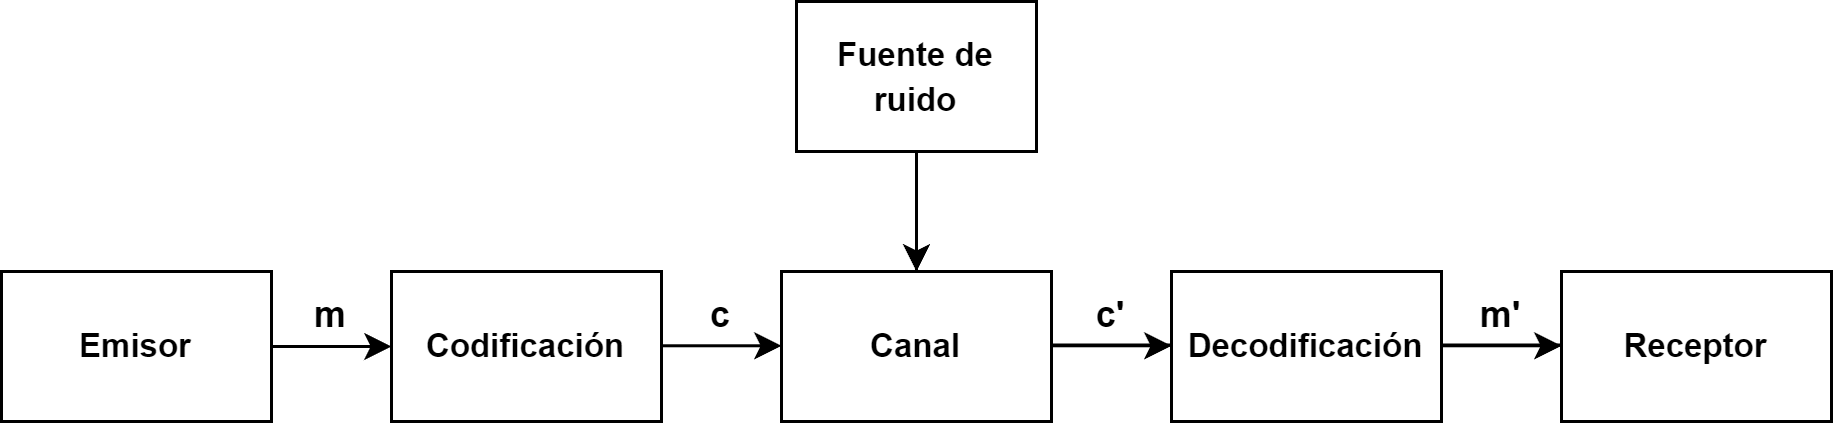
\includegraphics[width=1\textwidth]{img/comunicacion.png}
    \caption{Esquema del modelo de comunicación \cite{Podesta2006}.}
    \label{fig:comunicacion}
\end{figure}

En general, el mensaje enviado  y el mensaje recibido serán distintos. De esta forma, la teoría de códigos se encarga principalmente de los pasos de codificación y decodificación del diagrama anterior.

Algunas de las aplicaciones de la teoría de códigos son:

\begin{itemize}
    \item \emph{Comunicaciones digitales}: Se emplea en la telefonía móvil y redes de datos para asegurar la calidad y fiabilidad de las transmisiones.
    \item \emph{Almacenamiento de datos}: También es esencial el uso de códigos para garantizar la integridad de la información en discos duros, SSDs y medios ópticos como CDs y DVDs.
    \item \emph{Transmisiones por satélite}: Son imprescindibles también en todo tipo de transmisiones por satélite (televisión, GPS...), ya que protege de posibles interferencias atmosféricas.
    \item \emph{Criptografía}: Otro de sus usos más populares (y con el que a veces se confunde), es la criptografía. Por ejemplo, se utilizan en sistemas de cifrado asimétrico, como puede ser el criptosistema McEliece, que usa códigos de Goopa.
\end{itemize}


\paragraph{\spacedlowsmallcaps{Enfoque}}
\phantom{}

El objetivo principal de este trabajo es estudiar los códigos convolucionales cíclicos sesgados (SCCC) e implementar el algoritmo de Sugiyama para la decodificación de estos códigos. En consecuencia, el trabajo se enfocará en introducir las herramientas necesarias para poder abordar este objetivo. En cuanto a los fundamentos matemáticos necesarios, estudiaremos los anillos, los cuerpos finitos, los módulos y los anillos de polinomios sesgados. Para la teoría de códigos, veremos nociones básicas de los códigos de bloque, centrándonos en los códigos lineales y cíclicos. También hablaremos de códigos convolucionales, otra clase de códigos distinta a los de bloque, los cuales serán esenciales para la definición del objeto principal de este trabajo, los códigos convolucionales cíclicos sesgados.


\paragraph{\spacedlowsmallcaps{Estructura del trabajo}}
\phantom{}


Este trabajo consta de cinco capítulos y dos apéndices. En el primer capítulo, introduciremos los fundamentos matemáticos necesarios para desarrollar la teoría de códigos que se pretende abordar en este trabajo. En el segundo capítulo estudiaremos algunos de los fundamentos de los códigos de bloque, enfocándonos principalmente en los códigos lineales y cíclicos, presentando también el algoritmo de Sugiyama para la decodificación de códigos BCH, una subclase de los códigos cíclicos. En el tercer capítulo profundizaremos en los códigos convolucionales, explorando sus bases matemáticas y algunas de sus propiedades fundamentales. En el cuarto capítulo, veremos en primer lugar los polinomios de Ore, una estructura matemática que constituye la base de los códigos convolucionales cíclicos sesgados, que se introducen a continuación. Finalmente, en el quinto capítulo describimos el algoritmo de Sugiyama para la decodificación de códigos convolucionales sesgados Reed-Solomon.

En el primer apéndice, se detallará el código implementado en el trabajo, así como la estructura de este y los test realizados para probar su funcionamiento. En el segundo apéndice, se expondrá la planificación temporal del proyecto y una estimación de los costes del mismo.

\paragraph{\spacedlowsmallcaps{Objetivos principales del trabajo}}
\phantom{}

En cuanto al ámbito de las \emph{Matemáticas}, los objetivos de este trabajo son:

\begin{itemize}
    \item Estudiar las nociones básicas de la teoría de códigos lineales.
    \item Explorar los códigos convolucionales y su estructura algebraica, así como algunas de sus propiedades fundamentales.
    \item Investigar la noción de ciclicidad para los códigos convolucionales mediante los polinomios de Ore.
    \item Estudiar los códigos convolucionales sesgados Reed-Solomon.
    \item Exponer el algoritmo de Sugiyama para códigos convolucionales sesgados Reed-Solomon.
\end{itemize}

En cuanto a la \emph{Ingeniería Informática}, observemos que los objetivos anteriores se enmarcan en el campo de la Computación teórica. Además, otros objetivos más específicos son:

\begin{itemize}
    \item Implementar el algoritmo de Sugiyama para la decodificación de códigos BCH.
    \item Implementar un sistema de construcción de códigos convolucionales sesgados Reed-Solomon.
    \item Implementar un sistema de codificación de códigos convolucionales sesgados Reed-Solomon.
    \item Implementar el algoritmo de Sugiyama para la decodificación de códigos convolucionales sesgados Reed-Solomon.
\end{itemize}

\paragraph{\spacedlowsmallcaps{Principales fuentes consultadas}}
\phantom{}

Entre todas las fuentes bibliográficas consultadas, sobresalen las siguientes:

Para el estudio de las herramientas matemáticas del primer capítulo, \cite{knapp2006basic} y \cite{Huffman_Pless_2010} han resultado de utilidad.

En el segundo capítulo, \cite{Huffman_Pless_2010} y \cite{betten2006error} han sido fundamentales para el desarrollo de la teoría de códigos de bloque.

Para el capítulo tres, dedicado a los códigos convolucionales, las fuentes principales han sido \cite{Huffman_Pless_2010}, \cite{Forney1970}, \cite{Johannesson2015}, \cite{cccheide} y \cite{jl2020}.

En el capítulo cuatro, centrado en los códigos convolucionales cíclicos sesgados (SCCC), se han utilizado como referencias principales \cite{gluesingluerssen2019skewpolynomial} y \cite{jacobson1996} para los anillos de polinomios sesgados, además de \cite{cccheide}, \cite{SCCC} y \cite{gomez2017sugiyama} para los códigos convolucionales cíclicos sesgados.

Finalmente, el capítulo cinco, que aborda el algoritmo de decodificación Sugiyama para los códigos convolucionales sesgados Reed-Solomon, se basa en los resultados descritos en \cite{gomez2017sugiyama}. 

Para el desarrollo de la implementación y pruebas, ha sido relevante la documentación de SageMath \cite{SageMath2022} y Pytest \cite{pytest7.4.0}.






\endinput

               

% --------------------------------------------------------------------
% MAINMATTER
% --------------------------------------------------------------------
%\mainmatter % activa la numeración de capítulos, resetea la numeración de las páginas y usa números arábigos

%\setpartpreamble[c][0.75\linewidth]{%
%	\bigskip % Deja un espacio vertical en la parte superior
%  Si el trabajo se divide en diferentes partes es posible incluir al inicio de cada una de ellas un breve resumen que indique el contenido de la misma. Esto es opcional.
%}

\cleardoublepage
% !TeX root = ../libro.tex
% !TeX encoding = utf8

%\setchapterpreamble[c][0.75\linewidth]{%
%	\sffamily
%  Breve resumen del capítulo. TODO
%	\par\bigskip
%}

\chapter{Preliminares}\label{ch:primer-capitulo}

En este primer capítulo se introducirán las herramientas matemáticas necesarias para el desarrollo de la teoría de códigos que se pretende abordar en este trabajo. Empezaremos con una introducción a la teoría de anillos e ideales, comentando algunas de sus propiedades más importantes. Después, estudiaremos los cuerpos finitos, los cuales son esenciales para la construcción de códigos. También estudiaremos los cuerpos de fracciones, que serán fundamentales para la construcción de códigos convolucionales. Por último, se dará una breve introducción a la teoría de módulos.   

Muchos de estos resultados son muy conocidos y en la mayoría de los casos se omitirán las demostraciones de los mismos. Las principales fuentes consultadas para el desarrollo de este capítulo han sido \cite{knapp2006basic}y \cite{Huffman_Pless_2010}.

\section{Anillos}

\begin{definicion} \label{def:anillo}
    Un \emph{anillo} $(\mathcal{A},+,\cdot)$ es un conjunto $\mathcal{A}$ con dos operaciones binarias $\mathcal{A}\times \mathcal{A} \rightarrow \mathcal{A}$ \ llamadas suma $(+)$ y producto $(\cdot)$, que verifican las siguientes propiedades:

    \begin{enumerate}
        \item Propiedad asociativa de la suma: $$ a + (b + c) = (a + b) + c \ \ \forall a,b,c \in \mathcal{A}.$$
        \item Existencia de un elemento neutro de la suma: $$ \exists 0 \in A : 0 + a = a + 0 = a \ \ \ \forall a \in \mathcal{A}.$$
        \item Existencia de un elemento inverso para la suma: $$ \forall a \in \mathcal{A} \ \exists -a \in \mathcal{A} : a + (-a) = (-a) + a = 0.$$
        \item Propiedad conmutativa de la suma: $$ a + b = b + a \ \ \forall a,b \in \mathcal{A}.$$
        \item Propiedad asociativa del producto: $$ a \cdot (b\cdot c) = (a\cdot b)\cdot c \ \ \forall a,b,c \in \mathcal{A}.$$
        \item Propiedad distributiva del producto: $$ a\cdot(b+c) = a\cdot b + a\cdot c, \ \ (a+b)\cdot c = a\cdot c + b\cdot c \ \ \forall a,b,c \in \mathcal{A}.$$
    \end{enumerate}

    Diremos que un anillo es \emph{conmutativo} si se verifica: $$a\cdot b = b\cdot a \ \ \forall a,b \in \mathcal{A}.$$
\end{definicion}

Un tipo de anillo destacado es el siguiente.

\begin{definicion}
    Un anillo $\mathcal{A}$ se dice \emph{unitario} si existe un elemento $1 \in \mathcal{A}$ tal que \\ $a\cdot1 = 1\cdot a = a \ \ \forall a \in \mathcal{A}$. Lo denotaremos \emph{elemento unidad}.
\end{definicion}

El conjunto de los elementos unidad de un anillo forman un \emph{grupo} con respecto a la operación producto. A este grupo lo llamaremos \emph{grupo de unidades} de $\mathcal{A}$ y se denotará por $\mathcal{U}(\mathcal{A})$.

\begin{ejemplo} Algunos ejemplos de anillos son los siguientes.
    \begin{itemize}
        \item El conjunto de los números enteros $\mathds{Z}$ es un anillo conmutativo y unitario.
        \item Los enteros de Gauss $\mathds{Z}[i] = \{a + bi : a,b \in \mathds{Z}\}$ forman también un anillo conmutativo y unitario.
        \item El conjunto de las matrices cuadradas con coeficientes reales $\mathcal{M}_n(\mathbb{R})$ forman un anillo con las operaciones de la suma y el producto de matrices. Tiene elemento unidad (la matriz identidad) y es no conmutativo.
    \end{itemize}
\end{ejemplo}


Dado un anillo $\mathcal{A}$ unitario podría darse que el elemento neutro y el elemento unidad coincidan. En ese caso, el anillo $\mathcal{A}$ tendrá un único elemento y diremos que el anillo es \emph{trivial}. 

\begin{definicion}
Dado un elemento $a \in \mathcal{A}$ de un anillo unitario, diremos que es \emph{unidad} si existe otro elemento $a^{-1} \in \mathcal{A}$ de forma que $a\cdot a^{-1} = a^{-1}\cdot a = 1$. En tal caso, $a^{-1}$ es único y lo llamaremos \emph{elemento inverso} de $a$.
\end{definicion}

Claramente, el $0$ no puede tener elemento inverso, pues cualquier otro elemento que multipliquemos por él, nos dará como resultado $0$. 

\begin{definicion}
    Diremos que $\mathcal{A}$ es un \emph{anillo de división} si todo elemento $a \in \mathcal{A}$ distinto de $0$ tiene inverso.
\end{definicion}

\begin{definicion}
    Los \emph{divisores de cero} en un anillo $\mathcal{A}$ son los elementos $a,b \in \mathcal{A}$ tales que $a\cdot b = 0$.
\end{definicion}

Los anillos conmutativos con $1 \neq 0$ que no contengan divisores de cero se denominarán \emph{dominios de integridad} (DI).

En un dominio de integridad se da la propiedad de \emph{cancelación}.

\begin{proposicion}
    Sea $\mathcal{A}$ un dominio de integridad, entonces si $a \neq 0$ \ y \ $ax = ay$, se verifica $x = y$.
\end{proposicion}

\begin{proof}
    $ax = ay \Rightarrow a(x-y) = 0$, por ser $\mathcal{A}$ dominio de integridad y $a \neq 0$ se tiene que $x-y = 0 \Rightarrow x=y$.
\end{proof}

\begin{definicion}
Sea $\mathcal{A}$ un anillo unitario. Se define su \emph{característica} como el entero positivo más pequeño $n$ tal que $ 1 + {\overset {n)}{\ldots }}+1=0$. Si no existe tal $n$ se dice que la característica de $\mathcal{A}$ es $0$.
\end{definicion}

\begin{definicion}
    Un \emph{subanillo} $\mathcal{B}$ de $\mathcal{A}$ es un subconjunto $\mathcal{B} \subset \mathcal{A}$ que es anillo con las operaciones heredadas de $\mathcal{A}$.
\end{definicion}

\begin{definicion}
Dados $\mathcal{A},\mathcal{B}$ dos anillos unitarios, una aplicación $f: \mathcal{A} \rightarrow B$ se dice \emph{homomorfismo} de anillos si \ $\forall a,b \in \mathcal{A}$ se tiene:
$$f(a + b) = f(a) + f(b), f(ab) = f(a)f(b) \text{ y } f(1_\mathcal{A}) = 1_\mathcal{B}.$$
\end{definicion}

\begin{definicion}
Un subconjunto $I$ no vacío de un anillo $\mathcal{A}$ es un \emph{ideal por la izquierda} si:
    \begin{enumerate}
        \item $I$ es un subgrupo aditivo de $\mathcal{A}$.
        \item El producto por la izquierda de un elemento de $I$ por otro elemento de $\mathcal{A}$ está en $I$, es decir, $a\cdot x \in I$, $\forall (a,x) \in \mathcal{A} \times I.$
    \end{enumerate}
    Y es un \emph{ideal por la derecha si}: 
    \begin{enumerate}
        \item $I$ es un subgrupo aditivo de $\mathcal{A}$.
        \item El producto por la derecha de un elemento de $I$ por otro elemento de $\mathcal{A}$ está en $I$, es decir, $x\cdot a \in I$, $\forall (a,x) \in \mathcal{A} \times I.$
    \end{enumerate}
    Un \emph{ideal bilátero} es un ideal por la derecha y por la izquierda. En un anillo conmutativo, las nociones de ideal por la derecha, de ideal por la izquierda y de ideal bilátero coinciden y simplemente hablaremos de ideal.
\end{definicion}

\begin{definicion}
Diremos que un anillo $\mathcal{A}$ es simple si no contiene ideales biláteros distintos de $\mathcal{A}$ y $\{0\}$.
\end{definicion}

\begin{ejemplo} Algunos ejemplos de ideales son los siguientes.
    \begin{itemize}
        \item $\{0\}$ y $\mathcal{A}$ son ideales de $\mathcal{A}$. De hecho, si $1 \in I$, entonces $\mathcal{A} = I$.
        \item Sea $n\mathds{Z} = \{n\cdot a : a \in \mathds{Z}\}, n \in \mathds{N}$, el conjunto de los múltiplos de $n$. Entonces $n\mathds{Z}$ es un ideal, pues todo número entero multiplicado por $n$ es un múltiplo suyo.
    \end{itemize}
\end{ejemplo}

Dado un ideal bilátero $I$ de un anillo $\mathcal{A}$, es posible definir una relación de equivalencia. Sean $a,b \in \mathcal{A}$, la relación $a\R b \Leftrightarrow a - b \in I$ es de equivalencia. Esta relación nos permite definir el conjunto cociente $A/I$, de las clases de equivalencia obtenidas a través de ella. Dado un elemento $a \in I$, su clase de equivalencia viene dada por: $$ [a] = a + I = \{a + x : x \in I\}.$$

Las propiedades de ideal hacen que el conjunto cociente $A/I$ sea un anillo, al que llamaremos \emph{anillo cociente}, con las siguientes operaciones (que están bien definidas):
\begin{itemize}
    \item Suma: $(a + I) + (b + I) = (a + b) + I$.
    \item Producto $(a + I)\cdot(b + I) = (ab) + I$.
\end{itemize}

Un ideal puede ser generado por un \emph{subconjunto}. Sea $\emptyset \neq S \subset \mathcal{A}$ un subconjunto, entonces el ideal generado por $S$ en $\mathcal{A}$ es: 
$$I(S) = \{x_1h_1 + \cdots x_rh_r: h_i \in I, x_i \in \mathcal{A}\} \Leftrightarrow I(S) = \bigcap_{I_i \supset S} I_i. \ I_i \text{ ideal de }\mathcal{A}.$$
Es decir, $I(S)$ es el menor ideal de $\mathcal{A}$ que contiene a $S$.

    \begin{itemize}
    \item \emph{Ideal principal:} El ideal es generado por un elemento, $bA = (b) = \{ab : a \in \mathcal{A}\}$.
    \item \emph{Ideal finitamente generado:} El ideal es generado por un número finito de elementos, $S = \{b_1,\dots,b_n\}$: $$I(S) = (b_1,\dots,b_n)\mathcal{A} = \{x_1b_1 + \cdots + x_nb_n : x_i \in \mathcal{A}\}.$$
    \end{itemize}
\begin{definicion}
    Llamaremos \emph{dominio de ideales principales} (DIP) a un dominio de integridad en el que todos sus ideales son principales.
\end{definicion}


\begin{teorema}[Forma Normal de Smith]
Sea $R$ un dominio de ideales principales y sea $A \in \mathcal{M}_{k \times n}(R)$ una matriz no nula con coeficientes en $R$. Entonces $A = CDB$, donde $B \in GL_n(R), C \in GL_k(R)$ y $D \in \mathcal{M}_{k \times n}(R)$, con $$ D =
    \begin{pmatrix}
    \alpha_1 & 0      & \cdots & 0      & \cdots & 0 \\
    0        & \alpha_2 & \cdots & 0      & \cdots & 0 \\
    \vdots   & \vdots & \ddots & \vdots &        & \vdots \\
    0        & 0      & \cdots & \alpha_m & \cdots & 0 \\
    \vdots   & \vdots &        & \vdots & \ddots & \vdots \\
    0        & 0      & \cdots & 0      & \cdots & 0 \\
    \end{pmatrix}$$ para algún $m \leq \min\{n,k\}$ y elementos $\alpha_1,\dots,\alpha_m \in R$ no nulos tales que \\ $\alpha_i \ | \ \alpha_{i+1}$, $\forall i \in \{1,\dots,m-1\}.$
\end{teorema}

La matriz $D$ del teorema anterior recibe el nombre de la \emph{Forma Normal de Smith} de la matriz $A$.

\section{Cuerpos}

\begin{definicion}
    Un cuerpo $(K,+,\cdot)$ es un \emph{anillo conmutativo} $K$ cuyo grupo de unidades $\mathcal{U}(K)$ es $ K\setminus\{0\}$. Diremos que un cuerpo es \emph{finito} si tiene un número finito de elementos.
\end{definicion}

Observemos que estamos suponiendo que forzosamente un cuerpo nunca es el anillo trivial $\{0\}$. En general, los cuerpos finitos con $q$ elementos los denotaremos por $\mathbb{F}_q$.

\begin{definicion}
    Sea $F$ un subanillo de un cuerpo $K$, que es, a su vez, un cuerpo. Diremos que $F$ es un \emph{subcuerpo} de $K$. Se dice también que $F \leq K$ es una \emph{extensión de cuerpos}.
\end{definicion}


El siguiente teorema recoge algunas de las propiedades más básicas e importantes de los cuerpos finitos.

\begin{teorema}\label{th:cf}
    Sea $\mathbb{F}_q$ un cuerpo finito con $q$ elementos. Entonces se verifican las siguientes afirmaciones:
    \begin{enumerate}
        \item[(i)] $|\mathbb{F}_q| = p^n$, para algún número primo $p$ y algún entero positivo $n$.
        \item[(ii)]  $\mathbb{F}_q$ contiene al subcuerpo $\mathbb{F}_p$.
        \item[(iii)] $\mathbb{F}_q$ es un espacio vectorial sobre $\mathbb{F}_p$ de dimensión $n$ y hay $q^n$ vectores en el espacio vectorial de dimensión $n$ sobre $\mathbb{F}_p$.
        \item[(iv)]  $p\alpha = 0 \ \forall \alpha \in \mathbb{F}_q$.
        \item[(v)] $\mathbb{F}_q$ es único salvo isomorfismo. 
    \end{enumerate}
\end{teorema}

\begin{proposicion}\label{prop:bin}
    Sea $\mathbb{F}_q$ un cuerpo finito de característica $p$ y $n \in \mathds{N}$. Entonces: $$(a + b)^{p^{n}} = a^{p^{n}} + b^{p^{n}}, \ \ \ \forall a, b \ \in \mathbb{F}_q.$$
    $$(a - b)^{p^{n}} = a^{p^{n}} - b^{p^{n}}, \ \ \ \forall a, b \ \in \mathbb{F}_q.$$
\end{proposicion}

\begin{proof}

Por el Teorema del binomio, se puede desarrollar la $n$-ésima potencia de un binomio. De esta forma tenemos que 

\begin{equation}
\label{eq:bin}
    (a + b)^{p^{n}} =  \sum_{k=0}^{p^{n}} \binom{p^n}{k}a^{p^n-k}b^k = \binom{p^n}{0}x^{p^n} + \binom{p^n}{1}x^{p^n-1}y + \cdots + \binom{p^n}{p^n-1} xy^{p^n-1} + \binom{p^n}{p^n}y^{p^n}.
\end{equation}

Por otro lado, sabemos que 

\begin{equation}
    \binom{p^n}{k} = \frac{p^n!}{k!(p^n-k)!}.
\end{equation}

En consecuencia, $\binom{p^n}{k}$ es divisible por $p$ para $k \in \{1,\dots,p^n-1\}$.

Entonces, todos los coeficientes de la ecuación anterior, salvo el primero y el último, son múltiplos de $p$, y, por tanto, en virtud del Teorema \ref{th:cf}, su valor es $0$.

Así, $$(a + b)^{p^{n}} = a^{p^{n}} + b^{p^{n}}.$$

La segunda igualdad se prueba de forma análoga teniendo en cuenta que 

\begin{equation}
    (a - b)^{p^{n}} =  \sum_{k=0}^{p^{n}} \binom{p^n}{k}(-1)^ka^{p^n-k}b^k.
\end{equation}
\end{proof}

\subsection{Anillos de polinomios sobre cuerpos finitos}

\begin{definicion}
    Sea $\mathcal{A}$ un anillo conmutativo y $x$ un elemento que no pertenece a $\mathcal{A}$. Un polinomio con coeficientes en $\mathcal{A}$ es una expresión de la forma
    $$a_nx^n + a_{n-1}x^{n-1} + \cdots + a_1x + a_0, \ \ n \in \mathds{N}, a_0,\dots ,a_n \in \mathcal{A}.$$
\end{definicion}

Dado un anillo $\mathcal{A}$ denotaremos por $\mathcal{A}[x]$ al conjunto de todos los polinomios con coeficientes en $\mathcal{A}$.

\begin{definicion} Sea $\mathcal{A}$ un anillo y sean $p(x) = a_mx^m + \cdots + a_1x + a_0$ y $q(x) = b_nx^n + \cdots + b_1x + b_0$ dos elementos de $\mathcal{A}[x]$. Supongamos que $m \leq n$.

    \begin{enumerate}
        \item Se define la suma de los polinomios $p(x)$ y $q(x)$ como el polinomio $$p(x) + q(x) = b_nx^n + \cdots + b_{m+1}x^{m+1} + (a_m + b_m)x^m + \cdots + (a_1 + b_1)x + (a_0 + b_0).$$
        \item Se define el producto de los polinomios $p(x)$ y $q(x)$ como el polinomio $$p(x)q(x) = a_mb_nx^{m + n} + \cdots + (b_0a_2 + b_1a_1 + b_2a_0)x^2 + (b_0a_1 + b_1a_0)x + a_0b_0.$$

    \end{enumerate}
    
\end{definicion}

Se comprueba fácilmente que si $\mathcal{A}[x]$ es un anillo conmutativo, entonces $\mathcal{A}[x]$  \emph{es también un anillo conmutativo} con las operaciones que acabamos de definir. Además, podemos identificar al anillo $\mathcal{A}$ como los elementos de $\mathcal{A}[x]$ de la forma $p(x) = a$, $a \in \mathcal{A}$. Por tanto, $\mathcal{A}$ es un subanillo de  $\mathcal{A}[x]$.

Veamos ahora algunos conceptos referentes a polinomios.

\begin{definicion} Sea $\mathcal{A}$ un anillo conmutativo y $p(x) = a_nx^n + \cdots + a_1x + a_0 \in \mathcal{A}$.

    \begin{enumerate}
        \item Si $a_n \neq 0$ se dice que el polinomio $p(x)$ tiene grado $n$ y se representa como $\gr(p(x)) = n$. Cuando $p(x) = 0$, consideraremos que su grado es $-\infty$. 
        \item Al elemento $a_k \in \mathcal{A}$ se le llama \emph{coeficiente de grado} $k$.
        \item El coeficiente de grado $n$ de un polinomio de grado $n$ se llama \emph{coeficiente líder}.
        \item El coeficiente de grado $0$ de un polinomio se llama \emph{término independiente}.
        \item Un polinomio cuyo coeficiente líder valga $1$ se dice que es un \emph{polinomio mónico}.
    \end{enumerate}
\end{definicion}

\begin{proposicion} Sean $p(x),q(x) \in \mathcal{A}[x]$. Entonces:
\begin{align*}
    \gr(p(x) + q(x)) \leq& \max\{\gr(p(x)),\gr(q(x))\}, \\
    \gr(p(x)q(x)) \leq& \gr(p(x)) + \gr(q(x)).
 \end{align*}

\end{proposicion}

Una vez dada una pequeña introducción a los anillos de polinomios en anillos arbitrarios, vamos a enfocarnos en el caso que nos interesa para el desarrollo de este trabajo, es decir, cuando el anillo es un \emph{cuerpo finito}. El conjunto de polinomios con coeficientes en $\mathbb{F}_q$ se denota por $\mathbb{F}_q[x]$. Como ya se ha comentado en el caso general, este conjunto es un \emph{anillo conmutativo} y, de hecho, es un \emph{dominio de integridad}.
\\ \\
El anillo $\mathbb{F}_q[x]$ no solo juega un papel fundamental en la construcción de cuerpos finitos, sino también en la construcción de ciertas familias de códigos, como veremos a lo largo de este trabajo.

Sean $f(x)$ y $g(x)$ polinomios en $\mathbb{F}_q[x]$, diremos que $f(x)$ divide a $g(x)$ si existe un polinomio $h(x) \in \mathbb{F}_q[x]$ tal que $g(x) = f(x)h(x)$ y este hecho lo denotamos por $f(x) \ | \ g(x)$. El polinomio $f(x)$ se llama \emph{divisor o factor} de $g(x)$. 

El \emph{máximo común divisor} de $f(x)$ y $g(x)$, suponiendo que al menos uno de ellos no es nulo, es el polinomio mónico en $\mathbb{F}_q[x]$ de mayor grado que divide a ambos. El máximo común divisor de dos polinomios es \emph{único} y se denota como $\mcd(f(x),g(x))$. Diremos que $f(x)$ y $g(x)$ son \emph{coprimos} si $\mcd(f(x),g(x)) = 1$.


El siguiente resultado nos dará las bases para definir posteriormente el algoritmo de Euclides.

\begin{proposicion}\label{prop:div}
Sean $f(x), g(x) \in \mathbb{F}_q[x]$ con $g(x) \neq 0$. Se verifican:
\begin{enumerate}
    \item[(i)] (Algoritmo de la división) Existen polinomios $h(x),r(x) \in \mathbb{F}_q[x]$ únicos tales que $$ f(x) = g(x)h(x) + r(x), \ \ \ \ \gr(r(x)) < \gr(g(x)).$$
    \item[(ii)] Si $f(x) = g(x)h(x) + r(x)$, entonces $\mcd(f(x),g(x)) = \mcd(g(x),r(x))$.
\end{enumerate}
\end{proposicion}

Utilizando este resultado de manera recursiva podemos hallar el máximo común divisor de dos polinomios. Este procedimiento se conoce como \emph{algoritmo de Euclides} y es análogo a su versión para números enteros.



\begin{teorema}[Algoritmo de Euclides]\label{th:ae} Sean $f(x), g(x) \in \mathbb{F}_q[x]$ con $g(x) \neq 0$.
    \begin{enumerate}
        \item Realizar los siguientes pasos hasta que $r_n(x) = 0$ para algún $n$:
            \begin{align*}
                f(x)        &= g(x) h_1(x) + r_1(x), & &\text{donde } \gr(r_1(x)) < \gr(g(x)),\\
                g(x)        &= r_1(x) h_2(x) + r_2(x),& &\text{donde } \gr(r_2(x)) < \gr(r_1(x)),\\
                r_1(x)      &= r_2(x) h_3(x) + r_3(x),& &\text{donde } \gr(r_3(x)) < \gr(r_2(x)),\\
                            \vdots\\
                r_{n-3}(x)  &= r_{n-2}(x) h_{n-1}(x) + r_{n-1}(x),& &\text{donde } \gr(r_{n-1}(x)) < \gr(r_{n-2}(x)),\\
                r_{n-2}(x)  &= r_{n-1}(x) h_{n}(x) + r_{n}(x),& &\text{donde } r_n(x) = 0.
            \end{align*}
            Entonces, $\mcd(f(x),g(x)) = cr_{n-1}(x)$, donde $c \in \mathbb{F}_q$ es una constante para que $cr_{n-1}(x)$ sea mónico.
        \item Existen polinomios $a(x),b(x) \in \mathbb{F}_q[x]$ tales que $$ a(x)f(x) + b(x)g(x) = \mcd(f(x),g(x)).$$
    \end{enumerate}
    
\end{teorema}

Puesto que en el paso 1 el grado se reduce en al menos una unidad, podemos asegurar que la secuencia de pasos anterior acaba en algún momento.

\begin{proposicion}\label{prop:dip}
    Sea $\mathbb{F}_q$ un cuerpo, entonces $\mathbb{F}_q[x]$ es un dominio de ideales principales.
\end{proposicion}

\begin{proof}
    Sea $I$ un ideal de $\mathbb{F}_q[x]$. Si $I$ es trivial entonces es principal ya que $\{0\} = 0\mathbb{F_q}[x]$ y $\mathbb{F}_q[x] = 1\mathbb{F}_q[x]$.
    
    Supongamos que $I$ es un ideal no trivial de $\mathbb{F}_q[x]$. Sea $p(x)$ el polinomio de menor grado en $I\setminus\{0\}$. Como $I$ es un ideal, $p(x)\mathbb{F}_q[x] \subseteq I \subseteq \mathbb{F}_q[x]$.
    
    Si $p(x)$ es un elemento $p$ de $\mathbb{F}_q\setminus\{0\}$, entonces $p(x)\mathbb{F}_q[x] = \mathbb{F}_q[x] = I$. Por tanto, $I$ es un ideal principal, pues está generado por un único elemento.
    
    Si, por el contrario, $p(x) \notin \mathbb{F}_q$, sea $a(x) \in I$ un polinomio al que $p(x)$ no divide. Esto es, $p(x) \nmid a(x)$. Por el algoritmo de la División \ref{prop:div}, existen dos polinomios $q(x),r(x) \in \mathbb{F}_q[x]$ tales que $a(x) = p(x)q(x) + r(x)$ y $\gr(r(x)) < \gr(p(x)), r(x) \neq 0$.

    Sin embargo, 
    $$a(x), p(x) \in I \Rightarrow a(x), p(x)q(x) \in I \Rightarrow r = a(x) - p(x)q(x) \in I.$$

    Pero esto no es posible, puesto que habíamos dicho que $p(x)$ era el polinomio de menor grado en $I - \{0\}$. Hemos llegado a una contradicción. Así, $p(x) \ | \ a(x)$, $\forall a(x) \in I$. Por tanto, $I = p(x)\mathbb{F}_q[x]$ e $I$ es un ideal principal. 

\end{proof}

\subsection{Cuerpo de fracciones}

Los cuerpos de fracciones son un tipo particular de cuerpo, que cobrará importancia cuando estudiemos los códigos convolucionales.

Sea $D$ un dominio de integridad y consideremos en $D \times (D \backslash \{0\})$ la relación $(a,b) \R (c,d) \Leftrightarrow ad - bc = 0,$ que se comprueba trivialmente que es de equivalencia. Consideramos el conjunto cociente,
$$ \frac{D \times (D \backslash \{0\})}{\R},$$ denotamos la clase del par $(a,b)$ por $a/b$ y  definimos las operaciones
$$\frac{a}{b} + \frac{c}{d} = \frac{ad + bc}{bd}, \ \ \frac{a}{b}\cdot\frac{c}{d} = \frac{ac}{bd}$$ ($bd \neq 0$ por ser $D$ un dominio de integridad), que están bien definidas.

El cero es $0/b$, la unidad es $a/a$ y el inverso de $a/b (a \neq 0)$ es $b/a$. Con estas operaciones, $$ \frac{D \times (D \backslash \{0\})}{\R}$$ es un cuerpo, al que llamaremos \emph{el cuerpo de fracciones} de $D$. 

El cuerpo de fracciones de $D$ es el mínimo cuerpo que contiene a $D$.


\subsection{Elementos primitivos}

Cuando trabajamos con cuerpos finitos, necesitamos poder sumar y multiplicar de la manera más simple posible. Recordemos que por el Teorema \ref{th:cf}, sabemos que $\mathbb{F}_q$, donde $q = p^n$ con $p$ primo, es un espacio vectorial sobre $\mathbb{F}_p$ de dimensión $n$. De esta manera, la suma en $\mathbb{F}_q$ consistirá en la suma usual de $n$-tuplas sobre el cuerpo $\mathbb{F}_p$. Sin embargo, la multiplicación en $\mathbb{F}_q$ no es tan sencilla y por eso buscaremos una forma de expresar los elementos del cuerpo que simplifique esta operación.

El conjunto $\mathbb{F}_q^*$ de los elementos no nulos de $\mathbb{F}_q$ es un \emph{grupo}. El siguiente teorema nos será de utilidad.

\begin{teorema}\label{th:ep}
  Se verifican las siguientes afirmaciones:
  \begin{itemize}
    \item[(i)] El grupo $\F_q^*$ es cíclico con respecto a la multiplicación y tiene orden $q-1$.
    \item[(ii)] Si $\gamma$ es un generador de este grupo cíclico, entonces $$\mathbb{F}_q = \{0,1 = \gamma^0,\gamma,\gamma^2,\dots,\gamma^{q-2}\},$$ y $\gamma^i = 1$ si y solo si $(q-1) \ | \ i.$ 
  \end{itemize}  
\end{teorema}

Cada generador $\gamma$ de $\mathbb{F}_q^*$ se llama \emph{elemento primitivo} de $\mathbb{F}_q$. Cuando los elementos no nulos de un cuerpo finito se expresan como potencias de $\gamma$, la multiplicación en el cuerpo se realiza de forma sencilla teniendo en cuenta que 

$$\gamma^i\gamma^j = \gamma^{i+j} = \gamma^s, \text{   donde   } \ 0 \  \leq s \leq q-2 \text{  \  y  \  } i + j \equiv s \text{    (mod   }  \ q-1). $$

Sea $\gamma$ un elemento primitivo de $\mathbb{F}_q$, entonces $\gamma^{q-1} = 1$ por definición. De esta manera $(\gamma^i)^{q-1} = 1$ para $0 \leq i \leq q-2$ probando que los elementos de $\mathbb{F}_q^*$ son las raíces de $x^{q-1} - 1 \in \mathbb{F}_p[x]$ y, por tanto, de $x^q - x$. Como $0$ es raíz de $x^q - x$, se tiene el siguiente teorema.

\begin{teorema}\label{th:raiz}
Las raíces del polinomio $x^q - x \in \mathbb{F}_p[x]$ son los elementos de $\mathbb{F}_q.$
\end{teorema}

\begin{definicion}
    
Un elemento $\xi \in \mathbb{F}_q$ es una \emph{$n$-ésima raíz de la unidad} si $\xi^n = 1$. Además, si $\xi^s \neq 1$ para $s \in \{1, \dots, n-1\}$, diremos que es una \emph{$n$-ésima raíz primitiva de la unidad}.
\end{definicion}

Un elemento primitivo $\gamma$ de $\mathbb{F}_q$ es, por tanto, una $(q-1)$-ésima raíz primitiva de la unidad. Se deduce del Teorema \ref{th:ep} que el cuerpo $\mathbb{F}_q$ contiene una $n$-ésima raíz primitiva de la unidad si y solo si $n \ | \ (q-1)$, en cuyo caso $\gamma^{(q-1)/n}$ es una $n$-ésima raíz primitiva de la unidad.


\subsection{Automorfismos de cuerpos finitos}

La siguiente definición nos será de utilidad a la hora de trabajar con anillos de  polinomios de Ore.

\begin{definicion}
Un \emph{automorfismo} $\sigma$ de $\mathbb{F}_q$ es una biyección $\sigma : \mathbb{F}_q \rightarrow \mathbb{F}_q$ que verifica:
\begin{itemize}
    \item $\sigma(\alpha + \beta) = \sigma(\alpha) + \sigma(\beta) \ \ \forall \alpha,\beta \in \mathbb{F}_q.$
    \item  $\sigma(\alpha\beta) = \sigma(\alpha)\sigma(\beta) \ \ \forall \alpha,\beta \in \mathbb{F}_q.$
\end{itemize}
\end{definicion}

La aplicación $\sigma_p: \mathbb{F}_q \rightarrow \mathbb{F}_q $, donde $q = p^n$ con $p$ primo, definida como $\sigma_p(\alpha) = \alpha^p$, $\forall \alpha \in \mathbb{F}_q$, es un \emph{automorfismo}. Obviamente, $\sigma_p(\alpha\beta) = (\alpha\beta)^p = (\alpha)^p(\beta)^p = \sigma_p(\alpha)\sigma_p(\beta)$, y $\sigma_p(\alpha + \beta) = (\alpha + \beta)^p = (\alpha^p + \beta^p) = \sigma_p(\alpha) + \sigma_p(\beta)$, donde se ha usado la Proposición \ref{prop:bin}. Además, el núcleo de la aplicación es $\{0\}$ y, por tanto, es un automorfismo, al que se le denomina \emph{automorfismo de Frobenius}. De manera análoga, definimos $\sigma_{p^r}(\alpha) =  \alpha^{p^r}$.

El conjunto de automorfismos de $\mathbb{F}_q$ forma un grupo con respecto a la operación de composición de funciones. Este grupo se denota como Gal($\mathbb{F}_q$) y se llama el \emph{grupo de Galois} de $\mathbb{F}_q$. Así, definiremos el \emph{orden} de un automorfismo como el menor entero $n$ tal que $\sigma^n(\alpha) = \alpha$, $\forall \alpha \in \mathbb{F}_q$.

\begin{teorema}
    El grupo de Galois Gal($\mathbb{F}_q$), donde $p = q^n$ y $p$ es primo, es cíclico de orden $n$ y está generado por el automorfismo de Frobenius $\sigma_p$.
\end{teorema}

Dado un elemento $\alpha \in \mathbb{F}_q$, diremos que queda \emph{fijo} por un automorfismo $\sigma$ si $\sigma(\alpha) = \alpha$. El conjunto de los elementos de $\mathbb{F}_q$ que quedan fijos por un automorfismo $\sigma$ forma un subcuerpo de $\mathbb{F}_q$ y se denomina \emph{subcuerpo fijo de } $\mathbb{F}_q$ por $\sigma$, se denota por $\mathbb{F}_q^{\sigma}$.

\subsection{Clases ciclotómicas y polinomios minimales}\label{sec:ciclo}

Sea $\mathbb{E}$ una extensión de cuerpos finita de $\mathbb{F}_q$. Entonces $\mathbb{E}$ es un espacio vectorial sobre $\mathbb{F}_q$ y entonces $\mathbb{E} = \mathbb{F}_{q^t}$ para algún entero positivo $t$. Por el Teorema \ref{th:raiz}, cada elemento $\alpha$ de $\mathbb{F}_{q^t}$ es una raíz del polinomio $x^{q^t} - x$, luego, existe un polinomio mónico $M_{\alpha}(x) \in \mathbb{F}_q[x]$ cuyo grado es mínimo y contiene a $\alpha$ como raíz. Este polinomio se denomina \emph{polinomio minimal de } $\alpha$ sobre $\mathbb{F}_q$. En el siguiente teorema veremos algunos hechos elementales acerca de los polinomios minimales.

\begin{teorema}
Sea $\mathbb{F}_q \leq \mathbb{F}_{q^t}$ una extensión de cuerpos y sea $\alpha$ un elemento de $\mathbb{F}_{q^t}$ cuyo polinomio minimal es $M_{\alpha}(x) \in \mathbb{F}_q[x]$. Se verifican las siguientes afirmaciones:
\begin{itemize}
    \item[(i)] $M_{\alpha}(x)$ es irreducible en $\mathbb{F}_{q}$.
    \item[(ii)] Si $g(x)$ es cualquier polinomio en $\mathbb{F}_{q}[x]$ tal que $g(\alpha) = 0$, entonces $M_{\alpha}(x) \ | \ g(x)$.
    \item[(iii)] $M_{\alpha}(x)$ es único, es decir, existe un único polinomio mónico en $\mathbb{F}_q[x]$ de grado mínimo que tiene a $\alpha$ como raíz.
\end{itemize} 
\end{teorema}

Sea $f(x)$ un polinomio irreducible en $\mathbb{F}_q$ de grado $r$. Podemos considerar la extensión generada por una de las raíces de $f(x)$ y obtenemos el cuerpo $\mathbb{F}_{q^r}$. El siguiente teorema nos afirma que en dicho caso, todas las raíces de $f(x)$ están en $\mathbb{F}_{q^r}$.

\begin{teorema}
Sea $f(x)$ un polinomio mónico irreducible en $\mathbb{F}_{q}$ de grado $r$. Entonces:
\begin{itemize}
    \item[(i)] Todas las raíces de $f(x)$ están en $\mathbb{F}_{q^r}$ y en cualquier extensión de cuerpos de $\mathbb{F}_{q}$ generada por una de sus raíces.
    \item[(ii)] $f(x) = \prod_{i=1}^{r}(x-\alpha_i)$, donde $\alpha_i \in \mathbb{F}_{q^r}$, para $i \in \{1,\dots,r\}$.
    \item[(iii)] El polinomio $f(x)$ divide a $x^{q^r} - x$.
\end{itemize}
\end{teorema}

En particular, este teorema se verifica para los polinomios minimales $M_{\alpha}(x)$ en $\mathbb{F}_q$ dado que estos polinomios son mónicos e irreducibles.

\begin{teorema}\label{th:1.pm}
    Sea \( \mathbb{F}_q  \leq \mathbb{F}_{q^t} \) una extensión de cuerpos, y sea \( \alpha \) un elemento de \( \mathbb{F}_{q^t} \) con polinomio minimal \( M_{\alpha}(x) \) en \( \mathbb{F}_q[x] \). Se verifican las siguientes afirmaciones:
    \begin{itemize}
      \item[(i)] El polinomio \( M_{\alpha}(x) \) divide a \( x^{q^t} - x \).
      \item[(ii)] El polinomio \( M_{\alpha}(x) \) tiene raíces distintas que pertenecen a \( \mathbb{F}_{q^t} \).
      \item[(iii)] El grado de \( M_{\alpha}(x) \) divide a \( t \).
      \item[(iv)] $ x^{q^t} - x = \prod_{\alpha}M_\alpha(x)$, donde $\alpha$ varía entre un subconjunto de $\mathbb{F}_{q^t}$ de forma que enumera los polinomios minimales de todos los elementos de $\mathbb{F}_{q^t}$ una única vez.
      \item[(v)] $ x^{q^t} - x = \prod_{f}f(x)$, donde $f$ varía entre todos los polinomios mónicos irreducibles en $\mathbb{F}_q$ cuyo grado divide a $t$.
    \end{itemize}
    \end{teorema}

    \begin{definicion}
    Dos elementos de $\mathbb{F}_{q^t}$ son \emph{conjugados} en $\mathbb{F}_{q}$ si tienen el mismo polinomio minimal en $\mathbb{F}_{q}[x]$.
    \end{definicion}

    Será de importancia encontrar todos los conjugados de $\alpha \in \mathbb{F}_q$, es decir, las raíces de $M_\alpha(x)$. Sabemos por el Teorema \ref{th:1.pm} que todas sus raíces son distintas y están en $\mathbb{F}_{q^t}$. Podremos encontrar estas raíces con ayuda del siguiente teorema.

    \begin{teorema}
        Sea $f(x)$ un polinomio en $\mathbb{F}_q[x]$ y sea $\alpha$ una raíz de $f(x)$ en alguna extensión $\mathbb{F}_{q^t}$. Entonces:
        \begin{itemize}
            \item[(i)] $f(x^q) = f(x)^q$
            \item[(ii)] $\alpha^q$ es también una raíz de $f(x)$ en $\mathbb{F}_q$.
        \end{itemize} 
        
    \end{teorema}

    \begin{proof}
        \textit{(i). } Sea $f(x) = \sum_{i=0}^{m}a_ix^i$. Puesto que $q = p^n$, donde $p$ es la característica de $\mathbb{F}_q$, se tiene que aplicando la Proposición \ref{prop:bin}, $f(x)^q = \sum_{i=0}^{m}a_i^qx^{iq}$. Sin embargo, $a_i^q = a_i$, ya que por el Teorema \ref{th:raiz}, los elementos de $\mathbb{F}_q$ son las raíces de $x^q - x$, lo que prueba \textit{(i)}. En particular, $f(\alpha^p) = f(\alpha)^q = 0$, probando \textit{(ii)}.
    \end{proof}

 Aplicando iteradamente el teorema anterior obtenemos que $\alpha,\alpha^q,\alpha^{q^2},\dots$ son raíces de $M_\alpha(x)$. La secuencia anterior terminará tras $r$ términos, siendo $r$ el menos entero tal que $\alpha^{q^r} = \alpha$.

 Sea $\gamma$ un elemento primitivo de $\mathbb{F}_{q^t}$, entonces $\alpha = \gamma^s$ para algún $s$. Así, $\alpha^{q^r} = \alpha$ si y solo si $\gamma^{sq^r - s} = 1$. Por el Teorema \ref{th:ep}, $sq^r \equiv s \text{  (mod} \ \ q^t - 1)$. En base a esto, definimos la \emph{clase $q$-ciclotómica de $s$ módulo $q^t - 1$} como el conjunto

 $$C_s = \{s,sq,\dots,sq^{r-1}\} \text{  (mod} \ \ q^t - 1),$$

 donde $r$ es el entero positivo más pequeño tal que $sq^r \equiv s \text{  (mod} \ \ q^t - 1)$. Los conjuntos $C_s$ dividen el conjunto de enteros $\{0,1,\dots,q^t-2\}$ en conjuntos disjuntos.

 \begin{ejemplo}
Las clases $2$-ciclotómicas módulo $15$ son $C_0 = \{0\},C_1 = \{1,2,4,8\}, C_3 = \{3,6,12,9\}, C_5 = \{5,10\} \ \text{ y } \ C_7 = \{7,14,13,11\}$.
 \end{ejemplo}

Ahora sabemos que las raíces de $M_\alpha(x) = M_{\gamma^s}(x)$ contienen a $\{\gamma^i \ | \ i \in C_s\}$. De hecho, estas son todas las raíces. Por tanto, si conocemos el tamaño de $C_s$, sabremos el grado de $M_\alpha(x)$.

\begin{teorema}\label{th:1.ult}
    Si $\gamma$ es un elemento primitivo de $\mathbb{F}_{q^t}$, entonces el polinomio minimal de $\gamma^s$ en $\mathbb{F}_q$ es $$ M_{\gamma^s}(x) = \prod_{i \in C_s} (x - \gamma^i). $$
\end{teorema}

\section{Módulos}

\subsection{Conceptos básicos de módulos}

En esta sección veremos una estructura algebraica muy importante para el estudio de los códigos convolucionales: los módulos. Las principales fuentes para la redacción de esta sección han sido \cite{wisbauer1991foundations} y \cite{cccheide}.

Informalmente, un módulo es un ”espacio vectorial“  sobre un anillo y no sobre un cuerpo. Este anillo puede ser (o no) conmutativo.

\begin{definicion}
Sea $\mathcal{R}$ un anillo, entonces un $\mathcal{R}$-módulo por la izquierda $M$ es un grupo abeliano $(M,+)$ y una operación $\cdot : \mathcal{R} \times M \rightarrow M$ tales que $\forall r,s \in \mathcal{R}$, $\forall x,y \in  M$ se tiene:
\begin{enumerate}
    \item $(rs)x = r(sx)$.
    \item $(r + s)x = rx + sx$.
    \item $r(x + y) = rx + ry$.
    \item $1x = x$.
\end{enumerate}

La definición de los $\mathcal{R}$-módulos por la derecha es análoga, sólo que el anillo actúa \emph{por la derecha}, es decir, se define una multiplicación escalar de la forma $\cdot :  M \times \mathcal{R}  \rightarrow M$.
\end{definicion}

Cuando $\mathcal{R}$ es conmutativo, hablaremos simplemente de $\mathcal{R}$-módulos.

\begin{ejemplo} \label{ej:mod}
    Veamos algunos ejemplos de módulos.
    
    \begin{enumerate}
        \item Sea $V$ un espacio vectorial sobre un cuerpo $K$, entonces $V$ es un $K$-módulo.
        \item Sea $(\mathcal{A},+,\cdot)$ un anillo. Entonces, $\mathcal{A}$ es un módulo por la izquierda y por la derecha sobre sí mismo utilizando su producto.
    \end{enumerate}
    \end{ejemplo}

\begin{definicion}
Sea $M$ un $\mathcal{R}$-módulo por la izquierda. Un \emph{submódulo} $N$ de $M$ es un subgrupo de $(M,+)$ cerrado para la multiplicación con elementos en $\mathcal{R}$, es decir, $rn \in N$ para todo $r \in \mathcal{R}, n \in N$.
\end{definicion}

De esta forma, $N$ también es un $\mathcal{R}$-módulo con la operación $\cdot : \mathcal{R} \times N \rightarrow N.$

\begin{definicion}
Se dice que un $\mathcal{R}$-módulo $M$ es \emph{simple} si sus únicos submódulos son $\{0\}$ y $M$.
\end{definicion}

\begin{definicion}
Sea $M$ un $\mathcal{R}$-módulo, sean $N,N_1,N_2$ dos subconjuntos no vacíos de $M$ y sea $A \subset \mathcal{R}$. Entonces definimos:
$$N_1 + N_2 = \{n_1 + n_2 \ | \ n_1 \in N_1, n_2 \in N_2\} \subset M,$$
$$ AN = \left\{\sum_{i=1}^{k}a_in_i \ | \ a_i \in A, n_i \in N, k \in \N \right\} \subset M.$$
\end{definicion}

Si $N_1$ y $N_2$ son submódulos, entonces $N_1 + N_2$ es también un submódulo de $M$. Además, para un ideal por la izquierda $A \subset \mathcal{R}$, el producto $AN$ es siempre un submódulo de $M$.

\begin{definicion}
Sean $M_1,M_2$ submódulos de un $\mathcal{R}$-módulo $M$. Si $M = M_1 + M_2$ y $M_1 \cap M_2 = \{0\}$, entonces se dice que $M$ es una \emph{suma directa} de $M_1$ y $M_2$. Se denota como $M = M_1 \oplus M_2$. 
\end{definicion}

En este caso, cada $m \in M$ se calcula de forma única como $m = m_1 + m_2$, con $m_1 \in M_1$, $m_2 \in M_2$. Los submódulos $M_1$ y $M_2$ se llaman \emph{sumandos directos} de $M$.

\subsection{Módulos libres}

\begin{definicion}
Sea $M$ un $\mathcal{R}$-módulo por la izquierda y sea $I$ un conjunto arbitrario de índices. Diremos que un conjunto $\{e_i\ : i \in I\}$ \emph{genera} $M$ si cualquier elemento $m \in M$ puede escribirse como una combinación lineal $m = \sum_{i \in S} \lambda_ie_i$, siendo $S \subset I$ finito. Si además este conjunto es linealmente independiente, diremos que es una \emph{base} de $M$.
\end{definicion} 

\begin{teorema}
    Sea $M$ un $\mathcal{R}$-módulo. Equivalen las siguientes afirmaciones.

    \begin{itemize}
        \item[(i)] M tiene una base $\{e_i : i \in I\}$.
        \item[(ii)] $M \cong \bigoplus_{i \in I} \mathcal{R}$.
    \end{itemize}
\end{teorema}

\begin{definicion}
Un \emph{módulo libre} es un $\mathcal{R}$-módulo por la izquierda $M$ que posee una base. El \emph{rango} de $M$ es la cardinalidad de la base.
\end{definicion}

\subsection{El módulo $\F[t]^n$}

En el ejemplo \ref{ej:mod} vimos que un anillo es un módulo sobre sí mismo. 

Sea $\F[t]$ un anillo de polinomios con coeficientes en un cuerpo finito $\F$. Entonces, $$\F[t]^n := \{(v_1,\dots,v_n) \ | \ v_i \in \F[t], i=1,\dots,n\}.$$

En esta sección veremos dos resultados referentes a los submódulos y sumandos directos de $\F[t]^n$. Estos resultados pueden encontrarse en \cite{cccheide} y se omitirán las demostraciones.

\begin{proposicion}
Sea $V$ un submódulo de $\F[t]^n$. Se verifican las siguientes afirmaciones
\begin{itemize}
    \item[(i)] $V$ es un módulo libre y su rango es finito.
    \item[(ii)] Si $v_1,\dots,v_r \in \F[t]^n$ forman un conjunto generador de $V$, entonces $V =  Im(M) = \{uM \ | \ u \in \F[t]^r\}$ donde \begin{equation}\label{eq:modma} M := \left[ \begin{array}{c} v_1 \\ \vdots \\ v_r \end{array} \right]  \in \F[t]^{r \times n}. \end{equation} Llamaremos a $M$ matriz generadora de $V$.
    \item[(iii)] Sean $P \in  \F[t]^{r \times r}$ y $M$ como en (ii). Entonces $V = Im(PM) \Leftrightarrow P$ es invertible sobre $\F[t]$.
\end{itemize}
\end{proposicion}

\begin{proposicion} \label{prop:cc3}
Sea $V \subseteq \F[t]^n$ un submódulo y sea $v_1,v_2,\dots,v_r \in \F[t]^n$ un conjunto generador de $V$. Sea $M$ la matriz \eqref{eq:modma}. Equivalen las siguientes afirmaciones.
\begin{itemize}
    \item[(i)] $V$ es un sumando directo de $\F[t]^n$.
    \item[(ii)] Cualquier base de $V$ puede ser completada a una base de $\F[t]^n$ .
    \item[(iii)] La forma normal de Smith de $M$ está dada por la matriz $\left( \begin{array}{cc} I_k & 0 \\ 0 & 0 \end{array}\right)$, donde $k$ es el rango de $V$.
    \item[(iv)] Si $\{v_1,\dots,v_r\}$ es una base de $V$ (equivalentemente, si $r$ es el rango de $V$), entonces $M$ es invertible por la derecha.
    \item[(v)] Para todo $v \in \F[t]^n$ y todo $\lambda \in \F[t] \backslash \{0\}$ se tiene que \begin{equation}\label{eq:modu1} \lambda v \in V \Rightarrow v \in V.\end{equation}
    \item[(vi)] Existe una matriz $N \in \F[t]^{n \times 1}$ tal que $V = \ker N := \{v \in \F[t]^n \ | \ vN = 0\}$.
    \item[(vii)] Para todos los submódulos $W \in \F[t]^n$ con el mismo rango de $V$ se tiene que $$V \subseteq W \Rightarrow V = W.$$  
\end{itemize}

Una matriz con la propiedad (iii) se dirá que es básica.

\end{proposicion}

\endinput

% !TeX root = ../libro.tex
% !TeX encoding = utf8

%\setchapterpreamble[c][0.75\linewidth]{%
%	\sffamily
%  Breve resumen del capítulo. TODO
%	\par\bigskip
%}

\chapter{Códigos de bloque}\label{ch:segundo-capitulo}

En este capítulo trataremos algunos de los fundamentos de la teoría de códigos de bloque, centrándonos principalmente en los códigos lineales. Partiremos de la definición más básica de código, es decir, un subconjunto de un cuerpo finito. Después se definirá el concepto de código lineal, añadiendo a los códigos una estructura de espacio vectorial que nos permitirá utilizar herramientas más potentes propias del álgebra lineal. Por último, estudiaremos una subclase de los códigos lineales, los códigos cíclicos. Estos nos permitirán aplicar algoritmos de decodificación muy eficientes. Las principales fuentes consultadas para este capítulo han sido \cite{Huffman_Pless_2010} y \cite{betten2006error}.


\section{Códigos lineales}\label{sec:1.1}

Consideremos el espacio vectorial de todas las $n$-tuplas sobre el cuerpo finito $\mathds{F}_{q}$, que denotaremos $\mathds{F}_{q}^{n}$.

\begin{definicion}
 Un $(n,M)$-código $\mathcal{C}$ sobre el cuerpo $\mathds{F}_{q}$ es un subconjunto de $\mathds{F}_{q}^{n}$ de tamaño $M$. A los elementos de $\mathcal{C}$ los llamaremos \textit{palabras código}. A $n$ se le llama la \textit{longitud} del código. Normalmente, cada vector $(a_1,a_2,...,a_n) \in \mathds{F}_{q}^{n}$ lo escribiremos de forma más compacta como $a_1\dotsb a_n$.
\end{definicion}

\begin{ejemplo}
Un elemplo de código podría ser un (4,6)-código formado por los siguientes elementos:

$$ 1100, \quad		1011, \quad			1101, \quad			1110,	\quad		1111,	\quad		0001. $$
\end{ejemplo}
Sin ninguna estructura adicional, las propiedades de un código son limitadas. Por tanto, dotaremos al código de \emph{linealidad}. Esto nos permitirá aplicar herramientas matemáticas más potentes que nos hagan sacarle más provecho.

\begin{definicion}
$\mathcal{C}$ es un $[n,k]$-código lineal sobre $\mathds{F}_{q}$ si es un subespacio $k$-dimensional de $\mathds{F}_{q}^{n}$. 
\end{definicion}

De esta forma, un $[n,k]$-código lineal $\mathcal{C}$ tendrá $q^k$ elementos. Como veremos, la linealidad tiene varias ventajas a la hora de codificar y decodificar de manera más eficiente.

\begin{definicion}
 Una \emph{matriz generadora} para un $[n,k]$-código lineal $\mathcal{C}$ es cualquier matriz $G$ de dimensión $k \times n$ cuyas filas forman una base de $\mathcal{C}$.
\end{definicion}

En general, hay varias matrices generadoras para un código. Un conjunto de información de $\mathcal{C}$ es cualquier conjunto de $k$ columnas linealmente independientes de  $G$. Las demás $r=n-k$ columnas se denominan conjunto redundante y $r$ es la redundancia de $\mathcal{C}$.

Si las primeras $k$ columnas forman un \emph{conjunto de información}, el código tiene una única matriz generadora de la forma $[I_k \ \vert \ A]$, donde $I_k$ es la matriz identidad de dimensión $k$. Se dice que dicha matriz está en \emph{forma estándar}.

Debido a que un código lineal es un subespacio vectorial, sabemos que es el núcleo de una transformación lineal. Esta propiedad da pie a la siguiente definición.

\begin{definicion}
 Una matriz $H$ de dimensión $(n-k) \times n$ es una matriz de paridad para un $[n,k]$-código lineal $\mathcal{C}$ si cumple
  $$\mathcal{C} = \left\{\mathbf{x} \in \mathds{F}_{q}^{n} \ \vert \ H\mathbf{x^T} = 0\right\}. $$ 
\end{definicion}

Nótese que las filas de $H$ también serán linealmente independientes. En general, al igual que ocurría con las matrices generadoras, pueden existir varias matrices de paridad para $\mathcal{C}$. \\ El siguiente teorema nos da una de ellas cuando $\mathcal{C}$ tiene una matriz generadora en forma estándar.

\begin{teorema}\label{th:uno}
Si \ $ G = \left[ I_k \ \vert \ A \right] $  es una matriz generadora para un $[n,k]$-código lineal $\mathcal{C}$ en forma estándar, entonces $H = \left[ - A^T  \ \vert \ I_{n-k} \right]$ es una \emph{matriz de paridad} para $\mathcal{C}$.
\end{teorema}

\begin{proof}
Puesto que $HG^T = -A^T + A^T = 0$, se tiene que $\mathcal{C}$ está contenido en el núcleo de la transformación $\mathbf{x} \rightarrow H\mathbf{x}^T$. Como $H$ tiene rango $n-k$, esta transformación lineal tiene un núcleo de dimensión $k$, que coincide con la dimensión de $\mathcal{C}$. 
\end{proof}

\begin{ejemplo}\label{ej:1.6}
Consideramos la matriz $  G = \left[ I_4 \ \vert \ A \right] $, donde
$$ G = \left[\begin{array}{cccc|ccc}
1&0&0&0&0&1&1\\
0&1&0&0&1&0&1\\
0&0&1&0&1&1&0\\
0&0&0&1&1&1&1\\
\end{array}\right]
$$

es la matriz generadora en forma estándar de un $[7,4]$-código binario $\mathcal{H}_3$. Utilizando el Teorema \ref{th:uno}, una matriz de paridad para $\mathcal{H}_3$ es

$$H = [A^T \ \vert \ I_3] =  \left[\begin{array}{cccc|ccc}
0&1&1&1&1&0&0\\
1&0&1&1&0&1&0\\
1&1&0&1&0&0&1\\
\end{array}\right]. $$

Este código se llama $[7,4]$-\emph{código de Hamming}.

\end{ejemplo}

\subsection{Códigos duales}\label{sec:1.2}

Recordemos que la matriz generadora $G$ de un $[n,k]$-código $\mathcal{C}$ es simplemente una matriz cuyas filas forman una base del código visto como subespacio vectorial. Las filas de una matriz de paridad $H$ también son linealmente independientes y, por tanto, forman una base de algún espacio vectorial. Así, $H$ es la matriz generadora de un código, que llamaremos \emph{ dual u ortogonal} de $\mathcal{C}$ y lo denotaremos como $\mathcal{C}^{\bot}$. Nótese que $\mathcal{C}^{\bot}$ es un $[n,n-k]$-código. 
\\
Una forma alternativa de definir el código dual es usando el producto escalar. Recordemos que el producto escalar de dos vectores $\mathbf{x} = x_1\dots x_n, \mathbf{y} = y_1\dots y_n$ de $\mathds{F}_{q}^{n}$ se define como: $$\mathbf{x} \cdot \mathbf{y} = \sum_{i=1}^{n} x_iy_i.$$ Por tanto, otra definición alternativa es la siguiente.

\begin{definicion}
Dado un $[n,k]$-código $\mathcal{C}$, su \emph{código dual} $\mathcal{C}^{\bot}$ es
$$\mathcal{C}^{\bot} = \left\{ \mathbf{x} \in \mathds{F}_{q}^{n} \ \vert \ \mathbf{x} \cdot \mathbf{c} = 0, \ \forall c \in \mathcal{C} \right\}. $$ 
\end{definicion}

La siguiente proposición caracteriza a las matrices generadoras y de paridad de $\mathcal{C}^{\bot}$ en términos de las de $\mathcal{C}$.

\begin{proposicion}
Si $G$ y $H$ son las matrices generadoras y de paridad de $\mathcal{C}$, respectivamente, entonces $H$ y $G$ son las matrices generadoras y de paridad para $\mathcal{C}^{\bot}$ respectivamente.
\end{proposicion}

\begin{proof}
Se tiene que $$\mathbf{y} \in \mathcal{C}^{\bot} \Leftrightarrow  \mathbf{c} \cdot \mathbf{y} = 0, \forall c \in \mathcal{C} 
\Leftrightarrow (\mathbf{x}G) \cdot \mathbf{y} = 0, \forall \mathbf{x} \in \mathds{F}_{q}^{k} \Leftrightarrow \mathbf{x}G\mathbf{y}^T = 0, \forall \mathbf{x} \in \mathds{F}_{q}^{k} \Leftrightarrow G\mathbf{y}^T = \mathbf{0},$$ donde hemos utilizado que $rg(G) = k$.

Por tanto, $$\mathcal{C}^{\bot} = \left\{ \mathbf{y} \in \mathds{F}_{q}^{n} \ \vert \ G\mathbf{y}^T=\mathbf{0} \right\},$$ luego, $G$ es una matriz de paridad de $\mathcal{C}^{\bot}$.

Veamos ahora que H es una matriz generadora para $\mathcal{C}^{\bot}$. Puesto que $H\mathbf{c}^T = 0,  \forall c \in \mathcal{C}$ (por ser una matriz de paridad para $\mathcal{C}$), cada fila de $H$ está en $\mathcal{C}^{\bot}$. Utilizando que $H$ tiene $n-k$ filas linealmente independientes y $dim(\mathcal{C}^{\bot}) = n-k$, obtenemos que $H$ es una matriz generadora de $\mathcal{C}^{\bot}$.
\end{proof}

\begin{definicion}
Un código $\mathcal{C}$ es auto-ortogonal si $\mathcal{C} \subseteq \mathcal{C}^{\bot}$ y diremos que es auto-dual si $\mathcal{C} = \mathcal{C}^{\bot}$.
\end{definicion}

\begin{proposicion}
Un código auto-dual tiene longitud par y su dimensión es $n/2$.
\end{proposicion}

\begin{proof}
Si un $[n,k]$-código $\mathcal{C}$ tiene dimensión $k$, sabemos que su dual $\mathcal{C}^{\bot}$ tiene dimensión $n-k$. Si suponemos que es auto-dual, entonces $\mathcal{C} = \mathcal{C}^{\bot}$ y, por tanto, $n - k = k$. Así $n = 2k$, $n$ es par y la dimensión de $\mathcal{C}$ es $n/2$.
\end{proof}

\begin{ejemplo}
El $[4,2]$-código ternario $\mathcal{H}_{3,2}$, también llamado tetracódigo, tiene una matriz generadora $G$ en forma estándar dada por

$$G = \left[\begin{array}{cc|cc}
1&0&1&1\\
0&1&1&-1\\
\end{array}\right]. $$
Veamos que este código es auto-dual.

En primer lugar, comprobemos que es auto-ortogonal, es decir, si $\mathcal{C} \subseteq \mathcal{C}^{\bot}$. Dado $\mathbf{c} \in \mathcal{C}$, sabemos que $\mathbf{c}$ pertenece a $\mathcal{C}^{\bot}$ si
$$ G\mathbf{c}^T = \mathbf{0} \Leftrightarrow \mathbf{c}G^T = \mathbf{0}. $$

Así, como $c = xG, x \in \mathds{F}_{q}^{k}$, debemos comprobar que $GG^T = O$.

$$ GG^T = \left[\begin{array}{cccc}
1&0&1&1\\
0&1&1&-1\\
\end{array}\right]
\left[\begin{array}{cc}
1&0\\
0&1\\
1&1\\
1&-1
\end{array}\right]   = O.
$$ 

Por tanto, $\mathcal{H}_{3,2}$ es \emph{auto-ortogonal}. Además, dado que $dim(\mathcal{C}^{\bot}) = 8 - 4 = 4 = dim(\mathcal{C})$, $\mathcal{C}$ es también auto-dual.

\end{ejemplo}

\subsection{Pesos y distancias}\label{sec:1.4}

Al tratar de corregir errores, es esencial establecer algún criterio para medir cuán diferentes son las palabras \emph{transmitidas y las recibidas}. Además, un \emph{invariante} importante de un código $\mathcal{C}$ será la distancia mínima entre palabras código distintas.

\begin{definicion}
  La \emph{distancia de Hamming} $d(\mathbf{x,y})$ entre dos vectores $\mathbf{x,y} \in \mathds{F}_{q}^n$ se define como el número de coordenadas en las que $\mathbf{x}$ e $\mathbf{y}$ difieren.
\end{definicion}
Veamos que efectivamente es una distancia.

\begin{teorema}
  La función distancia $d(\mathbf{x,y})$ de Hamming satisface las siguientes propiedades:
  \begin{enumerate}
    \item[(i)] $d(\mathbf{x,y}) \geq 0 \ \forall \mathbf{x,y} \in \mathds{F}_{q}^n$ (no negatividad).
    \item[(ii)] $d(\mathbf{x,y}) = 0$ \emph{si y solo si} $\mathbf{x} = \mathbf{y}$.
    \item[(iii)] $d(\mathbf{x,y}) = d(\mathbf{y,x}) \ \forall \mathbf{x,y} \in \mathds{F}_{q}^n$ (simetría).
    \item[(iv)] $d(\mathbf{x,z}) \leq d(\mathbf{x,y}) + d(\mathbf{y,z}) \ \forall \mathbf{x,y,z} \in \mathds{F}_{q}^n$ (desigualdad triangular).
  \end{enumerate}
\end{teorema}

\begin{proof}

  Las tres primeras propiedades son evidentes. Veamos que se da la desigualdad triangular. Sean $\mathbf{x,y,z} \in \mathbb{F}_q^n$. Supongamos que $d(\mathbf{x},\mathbf{y}) = r$ y que $d(\mathbf{y},\mathbf{z}) = s$. Por tanto, $\mathbf{x}$ e $\mathbf y$ difieren en $r$ posiciones, digamos $i_1,i_2,\dots,i_r$. Análogamente, $\mathbf{z}$ e $\mathbf{y}$ difieren en las posiciones $j_1,j_2,\dots,j_s$. Entonces, todas las posiciones en las que $\mathbf{x}$ y $\mathbf{z}$ difieran tienen que estar en el conjunto $\{i_1,i_2,\dots,i_r,j_1,j_2,\dots,j_s\}$, que tiene como máximo $r+s$ elementos, lo que nos dice que 
  $$d(\mathbf{x},\mathbf{z}) \leq r + s = d(\mathbf{x},\mathbf{y}) + d(\mathbf{y},\mathbf{z})$$
  
\end{proof}

\begin{ejemplo}
  Sean $\mathbf{x} = 11001001$ e $\mathbf{y} = 11010111$ elementos de $\mathds{F}_{2}^8$, entonces su \emph{distancia de Hamming} es $d(\mathbf{x,y}) = 4$.
\end{ejemplo}

La \emph{distancia mínima} de un código $\mathcal{C}$ es la distancia más pequeña entre palabras código distintas. Es esencial a la hora de determinar la capacidad de corregir errores de $\mathcal{C}$ como veremos en el siguiente teorema. Si la distancia mínima $d$ de un $[n,k]$-código se conoce, nos referiremos al código como un $[n,k,d]$-código.

\begin{teorema}[Decodificación de máxima verosimilitud]\label{th:errores} Sea $\mathcal{C}$ un $[n,k,d]$-código. Entonces, $\mathcal{C}$ puede detectar hasta $d-1$ errores y puede corregir hasta $$ t = \left\lfloor \frac{d-1}{2} \right\rfloor $$

\end{teorema}

\begin{proof}
  Si hay menos de $d$ errores, debido a que la distancia mínima es $d$, no se obtendrá una palabra código, y, por tanto, podemos detectar hasta $d-1$ errores.
  Para la segunda parte, supongamos que se envía una palabra $\mathbf{u}$ y se recibe una palabra $\mathbf{v}$ con, a lo sumo, $t$ errores. Entonces $d(\mathbf{u,v}) \leq t$. Supongamos que existe otra palabra $\mathbf{w} \in \mathcal{C}$ tal que $d(\mathbf{u,w}) \leq t$, entonces utilizando la desigualdad triangular de la distancia de Hamming:
  $$d(\mathbf{v,w}) = d(\mathbf{v,u}) + d(\mathbf{u,w})  \leq 2t \leq d-1.$$
  Esto es una contradicción, puesto que recordemos que $d$ es la distancia mínima entre dos palabras código, por lo que $\mathcal{C}$ puede corregir hasta $t$ errores.
\end{proof}

De esta forma, nos interesará que la \emph{distancia mínima} sea lo mayor posible, con el fin de detectar el mayor número de errores.

Veamos otro concepto interesante relacionado con la distancia de Hamming.

\begin{definicion}
El \emph{peso de Hamming} $wt(x)$ de un vector $\mathbf{x} \in \mathds{F}_{q}^n$ es el número de coordenadas no nulas en $\mathbf{x}$.
\end{definicion}

\begin{ejemplo}
Sea $\mathbf{x} = 1101001$ un elemento de $\mathds{F}_{2}^7$, entonces $wt(\mathbf{x}) = 4$. Nótese que $wt(\mathbf{x}) = d(\mathbf{x,0}) = 4.$
\end{ejemplo}

La relación con la \emph{distancia de Hamming} se sigue del siguiente teorema.

\begin{teorema}\label{th:wp}
Sean $\mathbf{x,y} \in \mathds{F}_{q}^n$, entonces $d(\mathbf{x,y}) = wt(\mathbf{x-y})$. Además, si $\mathcal{C}$ es un código lineal, la distancia mínima $d$ coincide con el mínimo peso de Hamming de una palabra código no nula en $\mathcal{C}$.
\end{teorema}

\begin{proof}
La primera parte de la prueba es inmediata, ya que si tenemos dos elementos distintos, el número de coordenadas en las que difieren es el mismo que el número de coordenadas no nulas al restarlos, esto es $d(\mathbf{x,y}) = d(\mathbf{0,x-y}) = wt(\mathbf{x-y})$.
\\
Para la segunda parte, queremos ver que $$\min_{\mathbf{u,v} \in \mathcal{C}}{d(\mathbf{u,v})} = \min_{\mathbf{w}  \in \mathcal{C^*}}{wt(\mathbf{w})}.$$

Sean $\mathbf{u,v} \in \mathcal{C}$ palabras códigos cuya distancia es mínima, entonces por ser $\mathcal{C}$ un subespacio vectorial, se tiene que $\mathbf{u-v} \in \mathcal{C}$. De esta forma, $d(\mathbf{u,v}) = wt(\mathbf{u-v})$. Por tanto, $$\min_{\mathbf{w}  \in \mathcal{C^*}}{wt(\mathbf{w})} \leq \min_{\mathbf{u,v} \in \mathcal{C}}{d(\mathbf{u,v})}.$$
\\
Por otro lado, sea $\mathbf{w} \in \mathcal{C^*}$ la palabra código cuyo peso de Hamming es mínimo. Así, como $wt(\mathbf{w}) = d(\mathbf{0,w})$ tenemos
$$\min_{\mathbf{u,v} \in \mathcal{C}}{d(\mathbf{u,v})} \leq \min_{\mathbf{w} \in \mathcal{C^*}}{wt(\mathbf{w})}.$$

Y se consigue la igualdad deseada.
\end{proof}

Como consecuencia del teorema anterior, la \emph{distancia mínima} también se conoce como \emph{peso mínimo del código}.

Otra cota importante para códigos lineales es la \emph{cota de Singleton}.

\begin{teorema}[Cota de Singleton]\label{th:cotaS}
Sea $\mathcal{C}$ un $[n,k,d]$-código lineal sobre $\mathbb{F}_q$. Entonces, $$ d \leq n - k + 1.$$
\end{teorema}

\begin{proof}
Recordemos que $\mathcal{C}$ tiene $q^k$ palabras código de longitud $n$. Para cada palabra código $\mathbf{c} = c_1\cdots c_{k-1}\cdots c_n$ consideraremos 
únicamente las primeras $k-1$ componentes. Existen $q^{k-1}$ palabras de longitud $k-1$ en $\mathbb{F}_q^{k-1}$. Dado que tenemos un total de $q^k$ palabras código, deben existir dos palabras código que tengan las primeras $k-1$ componentes iguales. La distancia entre estas dos palabras código es $n - (k-1)$ y, por tanto, $d \leq n - (k - 1) = n - k + 1$.
\end{proof}

Los códigos que alcancen la cota de Singleton se denominan códigos MDS (máxima distancia separable).

\begin{definicion}
  Sea $A_i\mathcal{(C)}$ el número de palabras código de peso $i$ en $\mathcal{C}$. Para cada $0 \leq i \leq n$, la lista $A_i(\mathcal{C})$ se denomina \emph{distribución de pesos o espectro de pesos} de $\mathcal{C}$.
\end{definicion}

Una gran parte de la investigación en teoría de códigos ha sido el cálculo de la distribución de pesos de códigos específicos o de familias de códigos conocidas.

\begin{ejemplo}
Vamos a calcular la distribución de pesos del código binario $\mathcal{C}$ con la siguiente matriz generadora:
$$G = \left[\begin{array}{cccccc}
  1&1&0&0&0&0\\
  0&0&1&1&0&0\\
  0&0&0&0&1&1\\
  \end{array}\right]. $$

  Sea $\mathbf{x} = (x_1,x_2,x_3) \in \mathds{F}_{2}^3$. Entonces, 
  $$(x_1,x_2,x_3)\left[\begin{array}{cccccc}
    1&1&0&0&0&0\\
    0&0&1&1&0&0\\
    0&0&0&0&1&1\\
    \end{array}\right] = (x_1,x_1,x_2,x_2,x_3,x_3). $$

  y las palabras código serán las siguientes:

  $$ 000 \rightarrow 000000, \quad		001 \rightarrow 000011, \quad			010 \rightarrow 001100, \quad			011 \rightarrow 001111,$$
  $$ 100 \rightarrow 110000, \quad		101 \rightarrow 110011, \quad			110 \rightarrow 111100, \quad			111 \rightarrow 11111.$$

  Así, $\mathcal{C} = \{000000,000011,001100,001111,110000,110011,111100,11111\}$.

  Se tiene que la distribución de pesos es $A_0(\mathcal{C}) = A_6(\mathcal{C}) = 1 $, $A_2(\mathcal{C}) = A_4(\mathcal{C}) = 3 $. Normalmente, solo se listan los $A_i$ no nulos.
\end{ejemplo}

Algunos hechos elementales acerca de las \emph{distribuciones de pesos} están recogidos en el siguiente teorema.

\begin{teorema}
Sea $\mathcal{C}$ un $[n,k,d]$-código lineal sobre $\mathds{F}_q$. Entonces:
\begin{enumerate}
  \item[(i)] $A_0(\mathcal{C}) + A_1(\mathcal{C}) + \cdots + A_n(\mathcal{C}) = q^k$.
  \item[(ii)] $A_0(\mathcal{C}) = 1$ y $A_1(\mathcal{C}) = A_2(\mathcal{C}) = \cdots = A_{d-1}(\mathcal{C}) = 0$.
  \item[(iii)] Si $\mathcal{C}$ es un código binario que contiene la palabra código $\mathbf{1} = 11\cdots 1$, entonces $A_i(\mathcal{C}) = A_{n-i}(\mathcal{C})$ para $i \in \{0,\dots,n\}$.
\end{enumerate}
\end{teorema}

\begin{proof}
  \hphantom \\
  \begin{itemize} 
  \item La propiedad \textit{(i)} es evidente. Recordemos que el número total de palabras de un $[n,k]$-código lineal sobre $\mathds{F}_q$ es $q^k$, y el peso de cada una de las palabras va de $0$ hasta $n$.
  \item Para la propiedad \textit{(ii)}  sabemos que $A_0(\mathcal{C}) = 1$, ya que $\mathbf{0} \in \mathcal{C}$ (por ser un subespacio vectorial), como consecuencia, si se diese que $A_i(\mathcal{C}) \neq 0$ para algún $i \in \{1,\dots,d-1\}$ existiría una palabra cuyo peso es menor que $d-1$, pero entonces su distancia de Hamming respecto a $\mathbf{0}$ sería menor que $d$ lo que contradice la propia definición de $d$.
  \item Por último, veamos la propiedad \textit{(iii)} . Puesto que $\mathcal{C}$ es un subespacio vectorial y $\mathbf{1} \in \mathcal{C}$ se tiene que si $\mathbf{c} \in \mathcal{C}$, entonces  $\mathbf{1-\mathbf{c}} \in \mathcal{C}$. Obsérvese que $wt(\mathbf{1-c}) = n - wt(\mathbf{c})$. De esta manera, para cada palabra código $\mathbf{c}$ de peso $i$ existirá otra palabra código $\mathbf{1-c}$ de peso $n-i$, lo que concluye la demostración.
  \end{itemize}
\end{proof}

\subsection{Codificación de códigos lineales}\label{sec:1.3}

Sea $\mathcal{C}$ un $[n,k]$-código lineal sobre el cuerpo $\mathds{F}_{q}$ con matriz generadora $G$. Sabemos que este código tiene $q^k$ palabras código, que podemos hacer corresponder con $q^k$ mensajes.

La manera más simple de ver un mensaje es como una $k$-tupla $\mathbf{m}\in \mathds{F}_{q}^k.$ Este mensaje lo codificaremos como la palabra código $\mathbf{c} = \mathbf{m}G$. Si $G$ está en forma estándar, las primeras $k$ coordenadas de la palabra código $\mathbf{c}$ son los símbolos de información $\mathbf{m}$,mientras que los $n-k$ símbolos restantes serán los símbolos de paridad, que son símbolos redundantes añadidos a $\textbf{m}$ que nos ayudarán a recuperar el mensaje si ocurre algún error.

\begin{ejemplo}\label{ej:1.12}

  Sea $\mathcal{C}$ un $[6,3]$-código binario lineal con la siguiente matriz generadora:
  $$ G = \left[\begin{array}{cccccc}
    1&0&0&1&0&1\\
    0&1&0&1&1&0\\
    0&0&1&0&1&1\\
    \end{array}\right].
    $$
Dado un mensaje $\mathbf{m} = (x_1,x_2,x_3) \in \mathds{F}_{2}^3$ lo codificamos utilizando la matriz generadora $G$.
$$ (x_1,x_2,x_3) \left[\begin{array}{cccccc}
  1&0&0&1&0&1\\
  0&1&0&1&1&0\\
  0&0&1&0&1&1\\
  \end{array}\right] = (x_1,x_2,x_3,x_1 + x_2,x_2 + x_3,x_1 + x_3).$$

  Así, este código codifica de la siguiente forma: 

  $$ 000 \rightarrow 000000, \quad		001 \rightarrow 001011, \quad			010 \rightarrow 010110, \quad			011 \rightarrow 011101,$$
  $$ 100 \rightarrow 100101, \quad		101 \rightarrow 101110, \quad			110 \rightarrow 110011, \quad			111 \rightarrow 111000.$$

  Por tanto, $\mathcal{C} = \{000000,001011,010110,011101,100101,101110,110011,111000\}$.
\end{ejemplo}




Puede darse que la matriz generadora $G$ no esté en forma estándar, sin embargo, si existiera un conjunto de índices $i_1,i_2,\dots,i_k$ correspondientes a las columnas de la matriz $G$, de manera que la matriz $k \times k$ formada por esas $k$ columnas de $G$ es igual a $I_k$, se dice que la codificación es \emph{sistemática}. Equivalentemente, una codificación es \emph{sistemática} cuando el mensaje se encuentra incrustado íntegramente en el código (aunque sea de forma desordenada). Se observa que la codificación en el Ejemplo \ref{ej:1.12} es sistemática, ya que las tres primeras coordenadas del mensaje codificado corresponden con el mensaje original.
\\
Sin embargo, no todas las codificaciones son sistemáticas.

\begin{ejemplo}\label{ej:1.13}

    Sea $\mathcal{C}$ un $[2,4]$-código binario lineal cuya matriz generadora es
    $$ G = \left[\begin{array}{cccc}
      1&0&0&1\\
      1&1&1&1\\
      \end{array}\right].
      $$
  Dado un mensaje $\mathbf{m} = (x_1,x_2) \in \mathds{F}_{2}^2$ lo codificamos utilizando la matriz generadora $G$.
  $$ (x_1,x_2,x_3) \left[\begin{array}{cccc}
    1&0&0&1\\
    1&1&1&1\\
    \end{array}\right] = (x_1 + x_2,x_2,x_2,x_1 + x_2).$$

    Entonces, este código codifica de la siguiente forma: 

  $$ 00 \rightarrow 0000, \quad		01 \rightarrow 1111, \quad			10 \rightarrow 1001, \quad			11 \rightarrow 0110.$$

  Por tanto, $\mathcal{C} = \{0000,1111,1001,0110\}$.
\end{ejemplo}

Observamos en el Ejemplo \ref{ej:1.13} que no existe ningún conjunto de índices $i_1,i_2$ correspondientes a las columnas de la matriz $G$, de manera que esas columnas formen la matriz identidad $I_2$. Además, la codificación del mensaje $01$ es $1111$ que no contiene al mensaje original. Cuando esto ocurre se dice que la codificación es \emph{no sistemática}.

Acabamos de ver un método para codificar un mensaje $\mathbf{m}$ utilizando la matriz generadora de un código $\mathcal{C}$. En ocasiones, también es posible utilizar la matriz de paridad $H$ para este mismo fin. La forma más simple de hacerlo es cuando la matriz $G$ está en forma estándar $[I_k \ \vert \ A]$. En este caso,  el Teorema \ref{th:uno} nos asegura que $H = \left[ - A^T  \ \vert \ I_{n-k} \right]$. Supongamos que un mensaje $\textbf{m} = x_1\cdots x_k$ se codifica en la palabra código $c = c_1\cdots c_n$. Como $G$ está en forma estándar, $c_1\cdots c_k = x_1\cdots x_k$. Por tanto, necesitamos determinar los $n-k$ símbolos de paridad (símbolos redundantes) \ $c_{k+1}\cdots c_n$. Puesto que $\mathbf{0} = H\mathbf{c}^T = \left[ - A^T  \ \vert \ I_{n-k} \right]\mathbf{c}^T, A^T\mathbf{m}^T = [c_{k+1}\cdots c_n]^T$. Este método se puede generalizar cuando $G$ es un codificador sistemático.

\begin{ejemplo}
  Sea $\mathcal{C}$ el mismo código binario que en el Ejemplo \ref{ej:1.12}. Podemos utilizar el Teorema \ref{th:uno} para encontrar la matriz de paridad $H$ (puesto que $G$ está en forma estándar). Así, 
  $$ H = \left[\begin{array}{cccccc}
    1&1&0&1&0&0\\
    0&1&1&0&1&0\\
    1&0&1&0&0&1\\
    \end{array}\right].
    $$
  
  Recordemos que el ejemplo anterior, habíamos obtenido que dado un mensaje $\mathbf{m} = (x_1,x_2,x_3) \in \mathds{F}_{2}^3$, su codificación era la palabra código $\mathbf{c} = c_1\cdots c_n = \mathbf{m}G = (x_1,x_2,x_3,x_1 + x_2,x_2 + x_3,x_1 + x_3)$.

  Seguimos el proceso descrito para codificar $\mathbf{m}$ a partir de $H$. Puesto que $\mathbf{0} = H\mathbf{c}$, obtenemos el siguiente sistema:
   \begin{equation*}
      \begin{cases}
        c_1 + c_2 + c_4 = 0,\\
        c_2 + c_3 + c_5 = 0,\\
        c_1 + c_3 + c_6 = 0.
      \end{cases}
    \end{equation*}
  Como $G$ está en forma estándar, $c_1 c_2 c_3 = x_1 x_2 x_3$ y resolviendo este sistema, obtenemos la misma palabra código que con la matriz generadora.

  
\end{ejemplo}

Debido a la correspondencia uno a uno entre mensajes y palabras código, a veces nos puede interesar obtener el mensaje $\textbf{m}$ a partir de la palabra código $\textbf{c}$ mediante un proceso inverso a la codificación. Supongamos que $\mathbf{c} = \mathbf{m}G$. Si $G$ está en forma estándar, será fácil recuperar el mensaje original, simplemente tendremos que quedarnos con las primeras $k$ componentes de $\mathbf{c}$. Si $G$ no está en forma estándar, al existir una biyección entre las palabras código y los mensajes, existirá una matriz $K$ de dimensión $n \times k$ de manera que $GK = I_k$. Llamaremos a $K$ la \emph{inversa por la derecha de $G$}, la cual no es necesariamente única. De esta forma, puesto que $\mathbf{c} = \mathbf{m}G$, $\mathbf{c}K = \mathbf{m}GK = \mathbf{m}$ y se podrá recuperar el mensaje original.

\begin{ejemplo}

  Sea $\mathcal{C}$ un $[7,3]$-código lineal dado por la matriz generadora

  $$ G = \left[\begin{array}{ccccccc}
    1&0&1&1&0&1&1\\
    1&1&0&1&0&1&0\\
    0&0&1&1&1&1&0\\
    \end{array}\right].
    $$
  
 Codificamos el mensaje $\mathbf{m} = 110$ con el procedimiento visto anteriormente. Así, $\mathbf{c} = \mathbf{m}G = 0110001$.

  Si queremos obtener el mensaje $\mathbf{m}$ a partir de $\mathbf{c}$, en primer lugar calculamos la matriz inversa por la derecha de $G$, que en este caso es

  $$ K = \left[\begin{array}{ccc}
    1&0&1\\
    1&1&1\\
    0&0&1\\
    0&0&0\\
    0&0&0\\
    0&0&0\\
    0&0&0\\
    \end{array}\right].
    $$
  Así, el mensaje original vendrá dado por $$\mathbf{c}K = (0,1,1,0,0,0,1)\left[\begin{array}{ccc}
    1&0&1\\
    1&1&1\\
    0&0&1\\
    0&0&0\\
    0&0&0\\
    0&0&0\\
    0&0&0\\
    \end{array}\right] = (1,1,0) = \mathbf{m}.$$
\end{ejemplo}

\section{Códigos cíclicos}

En esta sección estudiaremos una clase destacada de códigos: los \emph{códigos cíclicos}. Estos códigos fueron introducidos en el año 1957 por Eugene Prange en \cite{prange1957cyclic}, que se percató de que los códigos cíclicos tenían una rica estructura algebraica. Esto sugirió que el álgebra podía desempeñar un papel crucial en la teoría de códigos. Los códigos cíclicos fueron unos de los primeros códigos usados en la práctica, ya que era fácil implementarlos utilizando registros de desplazamiento.
La principal fuente consultada para esta sección ha sido \cite{Huffman_Pless_2010}.

\begin{definicion}
Un código lineal $\mathcal{C}$ de longitud $n$ sobre $\mathbb{F}_q$ es \emph{cíclico} si para cada palabra código $\mathbf{c} = c_0\cdots c_{n-2}c_{n-1}$ en $\mathcal{C}$, el vector $c_{n-1}c_0\cdots c_{n-2}$, obtenido mediante un desplazamiento cíclico de $\mathbf{c}$, llevando $i \rightarrow i+1$ mod $n$, está también en $\mathcal{C}$.
\end{definicion}

Por tanto, dado un elemento $\mathbf{c}$ de un código cíclico $\mathcal{C}$, se tiene que los $n$ desplazamientos cíclicos de $\mathbf{c}$ también están en $\mathcal{C}$.

Normalmente, al estudiar los códigos cíclicos sobre $\mathbb{F}_q$ representaremos las palabras código en forma polinomial. Esto se debe a que existe una correspondencia biyectiva entre los vectores $\mathbf{c} = c_1\cdots c_{n-1} \in \mathbb{F}_{q}^n$ y los polinomios $c(x) = c_0 + c_1x + \cdots c_{n-1}x^{n-1} \in \mathbb{F}_q[x]$ de grado máximo $n-1$. Nótese que si $c(x) =  c_0 + c_1x + \cdots c_{n-1}x^{n-1}$, entonces $xc(x) =  c_{n-1}x^{n} + c_0x + c_1x^2 + \cdots c_{n-2}x^{n-1}$, que representaría a la palabra código $\mathbf{c}$ desplazada cíclicamente una posición a la derecha si $x^n$ fuese igual a $1$. 

Formalmente, el hecho de que un código $\mathcal{C}$ sea invariante bajo un desplazamiento cíclico, implica que si $c(x)$ está en $\mathcal{C}$, entonces $xc(x)$ también lo está, siempre que multipliquemos módulo $x^n-1$. Esto nos sugiere que el contexto adecuado para el estudio de los códigos cíclicos es el anillo cociente $$\mathcal{R}_n = \mathbb{F}_q[x]/\langle x^n-1 \rangle.$$
De esta manera, bajo la correspondencia de vectores con polinomios descrita anteriormente, los códigos cíclicos son \emph{ideales} de $\mathcal{R}_n$ y los ideales de $\mathcal{R}_n$ son códigos cíclicos. Así, el estudio de los códigos cíclicos en $\mathbb{F}_{q}^n$ es equivalente al estudio de los ideales en $\mathcal{R}_n$, que depende de la factorización de $x^n-1$, que estudiaremos a continuación.



\subsection{Factorización de $x^n-1$}

Nuestro primer objetivo será encontrar los factores irreducibles de $x^n-1$ sobre $\mathbb{F}_q$. Existen dos posibilidades: que $x^n-1$ tenga factores irreducibles repetidos o que no los tenga. Para el estudio de los códigos cíclicos nos centraremos en la segunda posibilidad. La siguiente proposición nos da una condición para que $x^n-1$ sobre $\mathbb{F}_q$ no tenga factores irreducibles repetidos.

\begin{proposicion}
Equivalen las siguientes afirmaciones:
\begin{enumerate}
    \item[(i)]$x^n-1$ no tiene factores irreducibles repetidos en $\mathbb{F}_q$.
    \item[(ii)] $mcd(q,n) = 1$.
\end{enumerate}
\end{proposicion}

\begin{proof}
   \phantom{a}\\ \\ \boxed{\text{\textit{(i)}} \Rightarrow \text{\textit{(ii)}}} 

    Supongamos que $x^n-1$ no tiene factores irreducibles repetidos sobre $\mathbb{F}_q$. Por reducción al absurdo, si $mcd(q,n) \neq 1$, entonces $n = q^em$ para algún $e > 0$, $q \nmid m$. De esta forma, 
    $$x^n - 1 = x^{q^em} - 1 = (x^{m})^{q^e} - 1 = (x^m - 1)^{q^e},$$ que claramente tiene factores irreducibles repetidos, lo cual supone una contradicción. Se ha utilizado la Proposición \ref{prop:bin}.
    \phantom{a}\\ \\ \boxed{\text{\textit{(ii)}} \Rightarrow \text{\textit{(i)}}} 

    Supongamos ahora que $mcd(q,n) = 1$. Sea $I$ el ideal de $\mathbb{F}_q[x]$ generado por los elementos $x^n - 1$ y $nx^{n-1}$. Por hipótesis, como $mcd(q,n) = 1$ se tiene que $n$, visto como un elemento de $\mathbb{F}_q$, es una unidad. Por tanto,

    $$nx^{n-1} \in I \Rightarrow x^{n-1} \in I \Rightarrow x^{n} \in I \Rightarrow x^n - (x^n - 1) \in I \Rightarrow 1 \in I \Rightarrow I = (1) =\mathbb{F}_q[x] .$$

    Por tanto, se tiene que en $\mathbb{F}_q[x]$, $mcd(x^n-1,nx^{n-1}) = 1$, ya que el ideal generado por ambos es el trivial. Recordemos que un polinomio $f\in \mathbb{F}_q[x]$ no tiene factores irreducibles repetidos si y solo si $mcd(f,f') = 1$. Utilizando este último resultado, donde $f = x^n - 1$, se concluye la demostración.

\end{proof}

Para factorizar $x^n - 1$ sobre $\mathbb{F}_q$ necesitamos encontrar una extensión de cuerpos $\mathbb{F}_{q^t}$ que contenga todas sus raíces. Dicho de otra forma, $\mathbb{F}_{q^t}$ debe contener una \emph{raíz n-ésima primitiva de la unidad}, que en virtud del Teorema \ref{th:ep}, esto ocurrirá si y solo si $ n \ | \ (q^t - 1)$. En tal caso, $\gamma^{(q^t - 1)/n}$ es dicha raíz.


\begin{definicion}
    El \emph{orden} de $q$ módulo $n$, denotado por $ord_n(q)$,  es el menor entero positivo $a$ tal que $q^a \equiv 1$ (mod $n$).
\end{definicion}

Nótese que si $t = ord_n(q)$, entonces $\mathbb{F}_{q^t}$ contiene una raíz n-ésima primitiva de la unidad $\alpha$, puesto que por la definición de orden, $q^t \equiv 1$ (mod $n$) $\Leftrightarrow n \ | \ (q^t - 1)$. Además, ninguna extensión de cuerpos más pequeña contendrá una raíz primitiva de la unidad, al ser $t$ el menor entero que cumple dicha condición. Como los $\alpha^i$ son distintos para $i \in \{0,\dots, n\}$ y $(\alpha^i)^n = 1$, $\mathbb{F}_{q^t}$ contiene todas las raíces de $x^n - 1$. En consecuencia, $\mathbb{F}_{q^t}$ es un \emph{cuerpo de descomposición} \footnote{Es decir, un cuerpo donde $x^n-1$ se factoriza mediante polinomios de grado uno.} de $x^n - 1$ sobre $\mathbb{F}_{q}$. De esta manera, los factores irreducibles de $x^n - 1$ sobre $\mathbb{F}_{q}$ deben ser el producto de los distintos polinomios minimales de las n-ésimas raíces de la unidad en $\mathbb{F}_{q^t}$. Supongamos que $\gamma$ es un elemento primitivo de $\mathbb{F}_{q^t}$. Entonces $\alpha = \gamma^d$ es una raíz n-ésima primitiva de la unidad, donde $d = (q^t - 1)/n$. Las raíces de $M_{\alpha^s}(x)$ son $$\{\gamma^{ds},\gamma^{dsq},\dots,\gamma^{dsq^{r-1}}\} = \{\alpha^s,\alpha^{sq},\dots,\alpha^{sq^{r-1}}\},$$ donde $r$ es el entero positivo más pequeño tal que $dsq^r \equiv ds \ \text{  (mod $q^t-1$)}$ por el Teorema \ref{th:1.ult}. Pero $dsq^r \equiv ds \ \text{  (mod $q^t-1$)}$ si y solo si $sq^r \equiv s \ \text{  (mod $n$)}$.

Esto nos lleva a extender la definición de clases $q$-ciclotómicas desarrolladas en la Sección \ref{sec:ciclo}.

Sea $s$ un entero, con $s \in \{0,\dots,n-1\}$. La clase $q$-ciclotómica de $s$ módulo $n$ es el conjunto
$$C_s = \{s,sq,\dots,sq^{r-1}\} \ \ \text{(mod }n),$$
donde $r$ es el entero positivo más pequeño tal que $sq^r \equiv s \ \ \text{(mod n)}$. En la Sección \ref{sec:ciclo} habíamos estudiado un caso más restrictivo, donde $n = q^t - 1$. Sin embargo, este concepto puede generalizarse a un $n$ arbitrario.

\begin{teorema}\label{th:fac}
Sea $n$ un entero positivo coprimo con $q$. Sea $t = ord_n(q)$. Sea $\alpha$ una $n$-ésima raíz primitiva de la unidad en $\mathbb{F}_{q^t}$.
\begin{itemize}
    \item[(i)] Para cada entero $s \in \{0,\dots,n-1\}$, el polinomio minimal de $\alpha^s$ en $\mathbb{F}_q$ es $$M_{\alpha^s}(x) = \prod_{i \in C_s}(x - \alpha^i), $$
    donde $C_s$ es la clase $q$-ciclotómica de $s$ módulo $n$.
    \item[(ii)] Los conjugados\footnote{Recordemos que dos elementos  son conjugados en $\mathbb{F}_{q}$ si tienen el mismo polinomio minimal en $\mathbb{F}_{q}[x]$.} de $\alpha^s$  son los elementos $\alpha^i$ con $i \in C_s$.
    \item[(iii)] Además, $$x^n - 1 = \prod_{s}M_{\alpha^s}(x)$$ es la factorización de $x^n - 1$ en factores irreducibles en $\mathbb{F}_q$, donde $s$ varía en un conjunto de representantes de las clases $q$-ciclotómicas módulo n.
\end{itemize}
\end{teorema}

\subsection{Teoría básica de códigos cíclicos}

Recordemos que los códigos cíclicos sobre $\mathbb{F}_q$ son precisamente los ideales de

$$\mathcal{R}_n = \mathbb{F}_q[x]/\langle x^n-1 \rangle.$$

La Proposición \ref{prop:dip} nos afirmaba que $\mathbb{F}_q[x]$ era un dominio de ideales principales. Veremos más adelante que los ideales de $\mathcal{R}_n$ también son principales, y, por tanto, los códigos cíclicos son los ideales principales de $\mathcal{R}_n$.

La manera más formal de escribir un código cíclico es como un elemento $c(x) + (x^n - 1)$ del ideal $\mathcal{R}_n$. Sin embargo, para simplificar la notación escribiremos $c(x)$. Así, pensaremos en los elementos de $\mathcal{R}_n$ como polinomios en $\mathbb{F}_q[x]$ en los que los términos de la forma $ax^{ni+j}$, $ j \in \{0,\dots,n-1\}, \ i \in \mathds{N}$, se cambiarán por $ax^j$. 

Para distinguir el ideal principal $(g(x))$ de $\mathbb{F}_q[x]$ del mismo ideal en $\mathcal{R}_n$, usaremos la notación $\langle g(x) \rangle$ para el ideal de $\mathcal{R}_n$ generado por $g(x)$. 

El siguiente teorema nos permitirá describir los códigos cíclicos, ya que nos afirma que hay una correspondencia biyectiva entre los códigos cíclicos en $\mathcal{R}_n$ y los polinomios mónicos que dividen a $x^n - 1$.

\begin{teorema}\label{th:ci}
Sea $\mathcal{C}$ un código cíclico no nulo en $\mathcal{R}_n$. Entonces existe un polinomio $g(x) \in \mathcal{C}$ que verifica las siguientes propiedades:
\begin{itemize}
    \item[(i)] $g(x)$ es el único polinomio mónico de grado mínimo en $\mathcal{C}$.
    \item[(ii)] El polinomio $g(x)$ genera $\mathcal{C}$. Es decir, $\mathcal{C} = \langle g(x) \rangle.$
    \item[(iii)] El polinomio $g(x)$ divide a $x^n-1$.
\end{itemize}
Sea $k = n- \gr(g(x))$ y sea $g(x) = \sum_{i=0}^{n-k}g_ix^i$ donde $g_{n-k} = 1$. Entonces:
\begin{itemize}
    
    \item[(iv)] La dimensión de $\mathcal{C}$ es $k$ y $\{g(x),xg(x),\dots,x^{k-1}g(x)\}$ es una base de $\mathcal{C}$.
    \item[(v)] Todo elemento de $\mathcal{C}$ se puede escribir de manera única como el producto de $g(x)f(x)$, donde $f(x) = 0$ o $\gr(f(x)) < k$.
    \item[(vi)] Una matriz generadora de $\mathcal{C}$ es
    
    $$ G =
    \left[\begin{array}{ccccccc}
    g_0 & g_1 & \cdots & g_{n-k} & & & \bigcirc \\
     & g_0 & g_1 & \cdots & g_{n-k} & & \\
     & & \ddots & \ddots & & \ddots & \\
    \bigcirc & & & g_0 &g_1 & \cdots &g_{n-k}
    \end{array}
    \right],
    $$

    donde cada fila es un desplazamiento cíclico de la fila anterior.


    \item[(vii)] Si $\alpha$ es una raíz $n$-ésima primitiva de la unidad en alguna extensión de $\mathbb{F}_q$, entonces  $$g(x) = \prod_{s}M_{\alpha^s}(x),$$
    siendo el producto sobre un subconjunto de representaciones de las clases $q$-ciclotómicas módulo $n$.
\end{itemize}
\end{teorema}

\begin{proof}
    \phantom{} \\ \\  \boxed{\textit{(i) y (ii)}} \\ \\ Sea $g(x)$ un polinomio mónico de grado mínimo en $\mathcal{C}$, que existe por ser $\mathcal{C}$ no nulo. Si $c(x) \in \mathcal{C}$, entonces, por el algoritmo de la división en $\mathbb{F}_q[x]$ \ref{prop:div}, $c(x) = g(x)h(x) + r(x)$, donde o bien $r(x) = 0$ o \ $\gr(r(x)) < \gr(g(x))$. Como $\mathcal{C}$ es un ideal de $\mathcal{R}_n$, $r(x) \in \mathcal{C}$ y al tener $g(x)$ grado mínimo, se deduce que $r(x) = 0$. Por tanto, $\mathcal{C} = \langle g(x) \rangle$, lo que prueba \textit{(ii)}. Si existiese otro polinomio $q(x)$ mónico de grado mínimo en $\mathcal{C}$ se tiene que $q(x) = g(x)h(x)$. Como $q(x)$ es mónico y del mismo grado que $g(x)$ necesariamente $h(x) = 1$ y, por tanto, $g(x) = q(x)$, lo que prueba \textit{(i)}.

    \boxed{\textit{(iii)}} \\ \\ Utilizando de nuevo el algoritmo de la división, $x^n - 1 = g(x)h(x) + r(x)$, donde $r(x) = 0$ o $\gr(r(x)) < \gr(g(x))$. Como en $\mathcal{R}_n$ se verifica que $x^n - 1 = 0 \in \mathcal{C}$, se tiene que $r(x) \in \mathcal{C}$, lo que es una contradicción a menos que $r(x) = 0$. En consecuencia, $ g(x) \ | \ x^n - 1$.

    \boxed{\textit{(iv) y (v)}} \\ \\
    Supongamos que $\gr(g(x)) = n-k$. Por los apartados \textit{(ii) y (iii)}, si $c(x) \in \mathcal{C}$ con $c(x) = 0$ o $\gr(c(x)) < n$, entonces $c(x) = g(x)f(x)$ para algún polinomio $f(x)$ en $\mathbb{F}_q[x]$. Si $c(x) = 0$, $f(x) = 0$. Por otro lado, $\gr(c(x)) < n$ implica que $\gr(f(x)) < k$. Entonces,  $$\mathcal{C} = \{g(x)f(x) \ | \ f(x) = 0 \text{ ó } \gr(f(x)) < k\}.$$
    Por tanto, $\mathcal{C}$ tiene dimensión al menos $k$ y $\{g(x),xg(x),\dots,x^{k-1}g(x)\}$ es un sistema de generadores de $\mathcal{C}$. Como estos $k$ polinomios tienen grados diferentes, son independientes en $\mathbb{F}_q[x]$. Además, tienen un grado estrictamente menor que $n$ y, por tanto, permanecen iguales en $\mathcal{R}_n$. Esto prueba que $\{g(x),xg(x),\dots,x^{k-1}g(x)\}$ es una base de $\mathcal{C}$ y que su dimensión es exactamente $k$, lo que nos lleva a \textit{(iv)}. De la unicidad de $g(x)$ se obtiene que la descomposición $c(x) = g(x)f(x)$ es única, lo que prueba \textit{(v)}.

    \boxed{\textit{(vi)}} \\ \\
    La matriz $G$ es matriz generadora de $\mathcal{C}$, ya que $\{g(x),xg(x),\dots,x^{k-1}g(x)\}$ es una base de $\mathcal{C}$.

    \boxed{\textit{(vii)}} \\ \\
    Se deduce del Teorema \ref{th:fac} y de \textit{(iii)}.
\end{proof}

Observemos que \textit{(ii)} prueba que $\mathcal{R}_n$ es un dominio de ideales principales, pues todos sus ideales (es decir, los códigos cíclicos) pueden ser generados por un único elemento. 

\begin{corolario}\label{col:ci}
Sea $\mathcal{C}$ un código cíclico no nulo en $\mathcal{R}_n$. Equivalen las siguientes afirmaciones;
\begin{itemize}
    \item[(i)] $g(x)$ es el polinomio mónico de menor grado en $\mathcal{C}$.
    \item[(ii)]  $\mathcal{C} = \langle g(x) \rangle$, $g(x)$ es mónico y divide a $x^n - 1$.
\end{itemize}
\end{corolario}

\begin{proof}
\phantom{} \\
\boxed{\textit{(i) $\Rightarrow$ \textit{(ii)}}} Probado en el Teorema \ref{th:ci}.


\boxed{\textit{(ii) $\Rightarrow$ \textit{(i)}}} \\

Sea $g_1(x)$ el polinomio mónico de menor grado en $\mathcal{C}$. Como se ha visto en la demostración del Teorema \ref{th:ci}, $g_1(x) \ | \ g(x)$ en $\mathbb{F}_q[x]$ y $\mathcal{C}= \langle g_1(x) \rangle $. Puesto que $g_1(x) \in \mathcal{C} = \langle g(x) \rangle$, se tiene que
$$ g_1(x) \equiv g(x)a(x) \text{   (mod  } x^n - 1).$$ 
También se tiene que $g_1(x) = g(x)a(x) + (x^n - 1)b(x)$ en $\mathbb{F}_q[x]$. Dado que $g(x) \ | \ (x^n - 1)$, entonces $g(x)$ divide a $g_1(x)$. Teniendo en cuenta que tanto $g_1(x)$ como $g(x)$ son mónicos y se dividen mutuamente en $\mathbb{F}_q[x]$, necesariamente son iguales.

\end{proof}

El Teorema \ref{th:ci} nos dice que existe un polinomio mónico $g(x)$ que divide a $x^n - 1$ y genera $\mathcal{C}$. El Corolario \ref{col:ci} asegura que $g(x)$ es único. A este polinomio le llamamos \emph{el polinomio generador} del código cíclico $\mathcal{C}$. Por el Corolario \ref{col:ci}, este polinomio es tanto el polinomio mónico en $\mathcal{C}$ de menor grado, como el polinomio mónico que divide a $x^n - 1$ y genera $\mathcal{C}$. Por tanto, existe una biyección entre los códigos cíclicos no nulos y los divisores propios\footnote{Entendemos por divisores propios de un polinomio al conjunto de todos sus divisores salvo él mismo.} de $x^n-1$. Para obtener la biyección entre el conjunto de los códigos cíclicos en $\mathcal{R}_n$ y el conjunto de divisores mónicos de $x^n - 1$,definimos el polinomio generador del código cíclico nulo $\{\mathbf{0}\}$ como $x^n - 1$, es decir, $\langle x^n - 1 \rangle = \{\mathbf{0}\}$ (recordemos que $x^n - 1 = 0$ en $\mathcal{R}_n$). Esta biyección nos conduce al siguiente corolario.

\begin{corolario}
El número de códigos cíclicos en $\mathcal{R}_n$ es igual a $2^m$, siendo $m$ el número de clases $q$-ciclotómicas módulo $n$.
\end{corolario}

Por tanto, si $g(x)$ es un polinomio de grado $n-k$ que divide a $x^n - 1$ en $\mathbb{F}_q[x]$, generará un $[n,k]$-código cíclico. Veamos un ejemplo de algún código cíclico.

\begin{ejemplo}
Dado el polinomio $x^9 - 1$, podemos factorizarlo en polinomios irreducibles en $\F_2[x]$ como $x^9 - 1 = (1 + x)(1 + x + x^2)(1 + x^3 + x^6)$.

Todos los divisores de $x^9 - 1$ generarán un código cíclico. En particular, veamos los códigos cíclicos $ \langle 1 + x\rangle$ y $ \langle 1 + x + x^2 \rangle$.

\begin{itemize}
    \item $\langle 1 + x \rangle:$ La dimensión del código es $k = 9 - 1 = 8$ y este polinomio genera un $[9,8]$-código cíclico. Haciendo uso del Teorema \ref{th:ci} podemos obtener la matriz generadora del código:
    $$ G = \left[\begin{array}{ccccccccc}
        1&1&0&0&0&0&0&0&0\\
        0&1&1&0&0&0&0&0&0\\
        0&0&1&1&0&0&0&0&0\\
        0&0&0&1&1&0&0&0&0\\
        0&0&0&0&1&1&0&0&0\\
        0&0&0&0&0&1&1&0&0\\
        0&0&0&0&0&0&1&1&0\\
        0&0&0&0&0&0&0&1&1\\
    \end{array}\right].$$
    \item $\langle 1 + x + x^2 \rangle:$ La dimensión del código es $k = 9 - 2 = 7$. Por tanto, este polinomio genera un $[9,8]$-código cíclico. Haciendo uso del Teorema \ref{th:ci} podemos obtener la matriz generadora del código:
    $$ G = \left[\begin{array}{ccccccccc}
        1&1&1&0&0&0&0&0&0\\
        0&1&1&1&0&0&0&0&0\\
        0&0&1&1&1&0&0&0&0\\
        0&0&0&1&1&1&0&0&0\\
        0&0&0&0&1&1&1&0&0\\
        0&0&0&0&0&1&1&1&0\\
        0&0&0&0&0&0&1&1&1\\
    \end{array}\right].$$
\end{itemize}
\end{ejemplo}

Los códigos cíclicos se pueden caracterizar a partir de los ceros del polinomio $x^n - 1$, es decir, a partir de las raíces n-ésimas de la unidad. Esta caracterización nos será de utilidad cuando estudiemos los códigos BCH.

Recordemos que el Teorema \ref{th:fac} nos dice que si $t = ord_n(q)$, entonces $\mathbb{F}_{q^t}$ es un cuerpo de descomposición del polinomio $x^n - 1$. Así, $\mathbb{F}_{q^t}$ contiene una raíz n-ésima primitiva de la unidad $\alpha$ y $x^n - 1 = \prod_{i=0}^{n-1}(x-\alpha^i)$ es la factorización de $x^n - 1$ en $\mathbb{F}_{q^t}$ mediante polinomios de grado uno. Además, $x^n - 1 = \prod_{s}M_{\alpha^s}(x)$ es la factorización de $x^n - 1$ utilizando polinomios irreducibles en $\mathbb{F}_q$ , donde $s$ varía en un conjunto de representantes de las clases $q$-ciclotómicas módulo $n$.

Sea $\mathcal{C}$ un código cíclico en $\mathcal{R}_n$ generado por el polinomio $g(x)$. Por los Teoremas \ref{th:fac} y \ref{th:ci}, el polinomio $g(x)$ se puede factorizar de la siguiente manera: \begin{equation}\label{eq:fac} g(x) = \prod_{s}M_{\alpha^s}(x) = \prod_{s}\prod_{i \in C_s}(x-\alpha^i),\end{equation} donde $s$, de nuevo, varía en un conjunto de representantes de las clases $q$-ciclotómicas módulo $n$. Sea $T = \bigcup_{s}C_s$ la unión de estas clases $q$-ciclotómicas, las raíces de la unidad $\mathcal{Z} = \{\alpha^i \ | \ i \in T \}$ se llaman \emph{ceros} del código cíclico $\mathcal{C}$ . El conjunto $T$ se denomina \emph{conjunto característico} de $\mathcal{C}$.

El siguiente teorema nos proporciona propiedades básicas de los códigos cíclicos a partir de sus conjuntos característicos.

\begin{teorema}\label{th:cc}
  Sea $\alpha$ una raíz $n$-ésima primitiva de la unidad en algún cuerpo de descomposición de $\mathbb{F}_q$ con conjunto característico $T$ y polinomio generador $g(x)$. Se verifican las siguientes afirmaciones:
  \begin{itemize}
    \item[(i)] El polinomio $g(x)$ se factoriza como $g(x) = \prod_{i \in T}(x - \alpha^i)$.
    \item[(ii)] La palabra código $c(x) \in \mathcal{R}_n$ está en $\mathcal{C}$ si y solo si $c(\alpha^i) = 0$, $\forall i \in T$.
    \item[(iii)]  La dimensión de $\mathcal{C}$ es $n - |T|$.
    \end{itemize}
\end{teorema}

\begin{proof}
  \phantom{} \\
  \begin{itemize}
    \item La propiedad \textit{(i)} se deduce fácilmente de \eqref{eq:fac} teniendo en cuenta que $T = \bigcup_{s}C_s$.
    \item Recordemos que por el Teorema \ref{th:ci}, $c(x)$ es múltiplo de $g(x)$. Además, este mismo teorema nos asegura que $g(\alpha^i) = 0$, $\forall i \in T$, lo que prueba \textit{(ii)}.
    \item La prueba de \textit{(iii)} es directa utilizando, de nuevo, el Teorema \ref{th:ci}, ya que por \textit{(i)},  $|T|$ es igual al grado del polinomio $g(x)$.
  \end{itemize}
\end{proof}

\section{Códigos BCH}

En esta sección estudiaremos una de las familias más importantes de códigos cíclicos: los códigos BCH. También estudiaremos una subfamilia de estos códigos, los códigos Reed-Solomon. Los códigos BCH fueron diseñados para aprovechar la \emph{cota de Bose-Ray-Chaudhuri-Hocquenghem}, abreviada como \emph{cota BCH}. La cota BCH dependerá de los ceros del código y, en particular, de la posibilidad de encontrar cadenas de ceros “consecutivas”.

En lo que sigue, consideraremos que $\mathcal{C}$ es un código cíclico de longitud $n$ en $\mathbb{F}_q$ y que $\alpha$ es una raíz $n$-ésima primitiva de la unidad en $\mathbb{F}_{q^t}$, donde $t = ord_n(q)$. Recordemos que $T$ es un conjunto característico de $\mathcal{C}$ siempre y cuando los ceros de $\mathcal{C}$ sean $\{\alpha^i \ | \ i \in T\}$. Por tanto, $T$ debe ser una unión de clases $q$-ciclotómicas módulo $n$. Diremos que $T$ contiene un subconjunto consecutivo de $s$ elementos $\mathcal{S}$ si existe un conjunto $\{b,b+1,\dots,b + s + 1\}$ de $s$ elementos consecutivos tal que 
$$\{b,b+1,\dots,b + s + 1\} \ \ \text{mod  }n = \mathcal{S} \subseteq T.$$

Antes de proceder con la cota BCH, enunciaremos un lema conocido que usaremos en la demostración de la cota.

Sean $\alpha_1,\dots,\alpha_s$ elementos de un cuerpo $\mathbb{F}$. Una matriz de la forma
$$
  V =
  \begin{pmatrix}
    1 & 1 & \cdots & 1 \\
    \alpha_1 & \alpha_2 & \cdots & \alpha_s \\
    \alpha_1^2 & \alpha_2^2 & \cdots & \alpha_s^2 \\
    \vdots & \vdots & \ddots & \vdots \\
    \alpha_1^{s-1} & \alpha_2^{s-1} & \cdots & \alpha_s^{s-1}
  \end{pmatrix}
$$
se llama \emph{matriz de Vandermonde} \footnote{A la transpuesta de $V$ también se le conoce como matriz de Vandermonde.}.

\begin{lema}\label{lm:Vand}
El determinante de una matriz de Vandermonde viene dado por $$ \det (V) = \prod_{1\leq i < j \leq s}(\alpha_j - \alpha_i).$$
En particular, $V$ es regular si los elementos $\alpha_1,\dots,\alpha_s$ son distintos.
\end{lema}

Ya tenemos las herramientas necesarias para demostrar el teorema de la cota BCH.

\begin{teorema}[Cota BCH]\label{th:cota}
Sea $\mathcal{C}$ un código cíclico de longitud $n$ sobre $\mathbb{F}_q$ y sea $T$ su conjunto característico. Supongamos que $\mathcal{C}$ tiene peso mínimo $d$ y que $T$ contiene $\delta - 1$ elementos consecutivos para algún entero $\delta$. Entonces $d \geq \delta$.
\end{teorema}

\begin{proof}

Sean $\alpha^b,\alpha^{b+1},\dots,\alpha^{b+\delta-2}$ los $\delta - 1$ ceros consecutivos de $\mathcal{C}$. Sea $c(x)$ una palabra código no nula en $\mathcal{C}$ cuyo peso de Hamming es $w$, de la forma
$$c(x) = \sum_{j=1}^{w}c_{i_j}x^{i_j}.$$
Supongamos que $w < \delta$. Como $c(\alpha^i) = 0$ para $i \in \{b,b+1,\dots,b+\delta - 2\}$, se tiene que $M\mathbf{u}^T = \mathbf{0}$, con 

$$M = \left[
\begin{array}{cccc}
\alpha^{i_1 b} & \alpha^{i_2b} & \cdots & \alpha^{i_wb} \\
\alpha^{i_1 (b+1)} & \alpha^{i_2(b+1)} & \cdots & \alpha^{i_w(b+1)} \\
\vdots & \vdots & \ddots & \vdots \\
\alpha^{i_1(b+w-1)} & \alpha^{i_2(b+w-1)} & \cdots & \alpha^{i_w(b+w-1)} \\
\end{array}
\right]$$
y $\mathbf{u} = (c_{i_1},c_{i_2},\dots,c_{i_w})$. Puesto que $\mathbf{u} \neq \mathbf{0}$, $M$ es una matriz singular, y, por tanto, $\det(M)=0$. Sin embargo, $\det(M) = \alpha^{(i_1+i_2+\cdots i_w)b}\det(V)$, donde $V$ es la matriz de Vandermonde 

$$V = \left[
\begin{array}{cccc}
1 & 1 & \cdots & 1 \\
\alpha^{i_1} & \alpha^{i_2} & \cdots & \alpha^{i_w} \\
\vdots & \vdots & \ddots & \vdots \\
\alpha^{i_1(w-1)} & \alpha^{i_2(w-1)} & \cdots & \alpha^{i_w(w-1)} \\
\end{array}
\right].$$
Como los $\alpha^{i_j}$ son distintos, $\det(V) \neq 0$ por el Lema \ref{lm:Vand}, lo que contradice que $\det(M) = 0$.
\end{proof}

Recordemos que la efectividad de un código $\mathcal{C}$ a la hora de corregir errores depende de su dimensión y de su peso mínimo, los cuales nos gustaría maximizar. Tener un peso mínimo grande, basándonos en la cota BCH, puede conseguirse eligiendo un conjunto característico $T$ de $\mathcal{C}$ con un gran número de elementos consecutivos. Puesto que por el Teorema \ref{th:cc} la dimensión de $\mathcal{C}$ es $n - |T|$, lo ideal sería que $|T|$ sea lo más pequeño posible. Así, si queremos que $\mathcal{C}$ tenga distancia mínima de al menos $\delta$, podemos elegir un conjunto característico tan pequeño como sea posible que sea unión de clases $q$-ciclotómicas con $\delta - 1$ elementos consecutivos.

\begin{definicion}
Sea $\delta \in \{2,\dots,n\}$.  Un \emph{código BCH} $\mathcal{C}$ sobre $\mathbb{F}_q$ de longitud $n$ y distancia mínima designada $\delta$ es un código cíclico con conjunto característico 
\begin{equation}\label{eq:bch}T = C_b \cup C_{b+1} \cup \cdots \cup C_{b+\delta-2},\end{equation} donde $C_i$ es la clase $q$-ciclotómica módulo n que contiene a $i$.
\end{definicion}

\begin{teorema}\label{th:bch}
Un código BCH de distancia mínima designada $\delta$ tiene peso mínimo de al menos $\delta$.
\end{teorema}

\begin{proof}
El conjunto característico \eqref{eq:bch} contiene $\delta - 1$ elementos consecutivos. El resultado se sigue de la cota BCH \ref{th:cota}.
\end{proof}

\subsection{Códigos Reed-Solomon}\label{subsec:rs}

Una subfamilia importante de los códigos BCH son los códigos Reed-Solomon, que abreviaremos como códigos RS.

\begin{definicion}
\emph{Un código Reed-Solomon (RS)} sobre $\mathbb{F}_q$ es un código BCH de longitud $n = q-1$.
\end{definicion}

De este modo, $ord_n(q) = 1$ implica que todos los factores irreducibles de $x^n-1$ son de grado uno y todas las clases $q$-ciclotómicas módulo $n$ tienen tamaño $1$. El siguiente teorema nos da algunas propiedades de los códigos RS.

\begin{teorema}
Sea $\mathcal{C}$ un código RS sobre $\mathbb{F}_q$ de longitud $n = q-1$ y distancia mínima designada $\delta$. Entonces:
\begin{itemize}
  \item[(i)] El código $\mathcal{C}$ tiene un conjunto característico de la forma $T = \{b,b+1,\dots,b+\delta-2\}$.
  \item[(ii)] El código $\mathcal{C}$ tiene distancia mínima $d = \delta$ y dimensión $k = n-d+1$. 
\end{itemize}
\end{teorema}

\begin{proof}
Veamos la demostración por apartados.
\begin{itemize} 
  \item La propiedad \textit{(i)} se deduce teniendo en cuenta que al ser un código BCH de distancia mínima designada $\delta$, su conjunto característico $T$ tiene que tener tamaño $\delta - 1$ y en consecuencia $T = \{b,b+1,\dots,b+\delta-2\}$.
  \item El Teorema \ref{th:cc} nos dice que la dimensión de $\mathcal{C}$ es $k = n - |T| = n - \delta + 1$. Además, la cota de Singleton \ref{th:cotaS} y el Teorema \ref{th:bch} nos aseguran que $k = n - \delta + 1 \geq n - d + 1 \geq k$, y, por tanto, $k = n - d + 1$, lo que prueba \textit{(ii)}.
\end{itemize}
\end{proof}

\section{Decodificación de códigos BCH con el algoritmo de Sugiyama}\label{sec:sugiyama}

En esta sección vamos a ver un algoritmo de decodificación para códigos BCH, el conocido \emph{algoritmo de Sugiyama}. Este algoritmo fue creado por Sugiyama, Kasahara, Hirasawa y Namekawa en 1975 \cite{sugiyama1975method}. Se diseñó para una clase de códigos llamada la clase de los códigos de Goopa, los cuales incluyen a los códigos BCH como una subclase suya. Sin embargo, en esta sección solo lo aplicaremos a códigos BCH. Este algoritmo es una aplicación del algoritmo de Euclides para polinomios \ref{th:ae}.
 
Sea $\mathcal{C}$ un código BCH sobre $\mathbb{F}_q$ de longitud $n$, distancia designada $\delta$ y conjunto característico $T$, con $\{b,b+1,\dots,b + \delta - 2\} \subseteq T$. Puesto que la distancia mínima de $\mathcal{C}$ es al menos $\delta$, por el Teorema \ref{th:errores}, $\mathcal{C}$ puede corregir hasta $ t = \left\lfloor \frac{\delta-1}{2} \right\rfloor $ errores. El algoritmo de Sugiyama nos permitirá corregir estos $t$ errores.

Como en cualquier algoritmo de decodificación, si suponemos que recibimos un mensaje $y(x)$, nosotros queremos obtener la palabra código original $c(x)$. Supondremos que $y(x)$ difiere de $c(x)$ a lo sumo en $t$ coordenadas. Por tanto, $$y(x) = c(x) + e(x),$$ donde $e(x)$ es el \emph{vector de errores} cuyo peso de Hamming es $\nu \leq t$. Supongamos que los errores ocurren en unas coordenadas desconocidas $k_1,k_2,\dots,k_{\nu}$. Entonces: \begin{equation}\label{eq:error}e(x) = e_{k_1}x^{k_1} + e_{k_2}x^{k_2} + \cdots  e_{k_{\nu}}x^{k_{\nu}}\end{equation}
Una vez determinemos el vector de errores $e(x)$, lo que equivale a encontrar las coordenadas de error $k_j$ y las magnitudes del error $e_{k_j}$, \  $j \in \{1,\dots,\nu \}$, podremos decodificar el vector recibido como $c(x) = y(x) - e(x)$. Recordemos que por el Teorema \ref{th:cc}, $c(x) \in \mathcal{C}$ si y solo si $c(\alpha^i) = 0$ para todo $i \in T$. En particular, dado que $t = \left\lfloor \frac{\delta-1}{2} \right\rfloor$ y que $T$ contiene a $\{b,b+1,\dots,b + \delta - 2\}$, se tiene que $$y(\alpha^i) = c(\alpha^i) + e(\alpha^i) = e(\alpha^i), \ \ \forall i \in \{b,b+1,\dots,b + 2t - 1\}.$$
Para $i \in \{b,b+1,\dots,b + 2t - 1\}$ definimos \emph{el síndrome} $S_i$ de $y(x)$ como el elemento  $S_i = y(\alpha^i)$ en $\mathbb{F}_{q^m}$.

El primer paso del algoritmo de Sugiyama será calcular los síndromes para un vector $y(x)$ que se ha recibido. Estos síndromes nos conducen a un sistema de ecuaciones que involucran tanto a las coordenadas de error desconocidas como a las magnitudes de error. Nótese que de \eqref{eq:error} los síndromes satisfacen \begin{equation}\label{eq:sin}
  S_i = y(\alpha^i) = e(\alpha^i) = \sum_{j=1}^{\nu}e_{k_j}(\alpha^i)^{k_j} = \sum_{j=1}^{\nu}e_{k_j}(\alpha^{k_j})^{i}, \ \ i \in \{b,b+1,\dots,b + 2t - 1\}.
\end{equation}

Con el objetivo de simplificar la notación, para $j \in \{1,\dots,\nu\}$ definimos:
\begin{itemize}
  \item $E_j = e_{k_j}$, que será la magnitud del error en la coordenada $k_j$.
  \item $X_j = \alpha^{k_j}$, que llamaremos número de coordenadas de error correspondiente a la coordenada de error $k_j$.
\end{itemize}

Por el Teorema \ref{th:ep}, si $\alpha^i = \alpha^k$ con $i \in \{0,\dots,n-1\}$, entonces $i = k$. Por tanto, conociendo $X_j$ conoceremos también la coordenada de error $k_j$. Con la notación anterior, \eqref{eq:sin} se puede expresar como:

\begin{equation}\label{eq:sin2}
  S_i = \sum_{j=1}^{\nu}E_jX_j^i, \ \ i \in \{b,b+1.\dots,b + 2t - 1\}.
\end{equation}

La expresión anterior nos conduce al sistema de ecuaciones

\begin{equation}
  \label{eq:sistema}
  \begin{cases}
    S_b = E_1X_1^b + E_2X_2^b + \cdots + E_{\nu}X_{\nu}^b ,\\
    S_{b+1} = E_1X_1^{b+1} + E_2X_2^{b+1} + \cdots + E_{\nu}X_{\nu}^{b+1},\\
    S_{b+2} = E_1X_1^{b+2} + E_2X_2^{b+2} + \cdots + E_{\nu}X_{\nu}^{b+2},\\
    \ \ \ \ \ \  \ \ \  \ \ \  \ \ \  \ \ \  \ \ \  \ \ \ \vdots \\
    S_{b + 2t - 1} = E_1X_1^{b + 2t - 1} + E_2X_2^{b + 2t - 1} + \cdots + E_{\nu}X_{\nu}^{b + 2t - 1}.\\
  \end{cases}
\end{equation}

Este sistema es no lineal para los $X_j$, y además, desconocemos tanto los valores de los $E_j$ como de los $X_j$. La estrategia será calcular directamente los números de coordenadas de error. Una vez conozcamos los $X_j$, volveremos al sistema \eqref{eq:sistema}, que será un sistema lineal formado únicamente por los $E_j$. Para este fin, definimos el \emph{polinomio localizador de errores} como $$\sigma(x) = \prod_{j=1}^{\nu}(1 - xX_j) =  (1- xX_1)(1 - xX_2)\cdots(1- xX_{\nu}) = 1 + \sum_{i=1}^{\nu}\sigma_ix^i.$$

Nótese que $\sigma(x) = 0$ si y solo si $x = X_j^{-1}$, $j \in \{1,\dots,\nu\}$. Por tanto, calculando las raíces del polinomio localizador de errores, calcularemos los inversos de los números de coordenadas de error, y podremos obtener los $X_j$ fácilmente.

\begin{definicion}
El \emph{polinomio evaluador de errores} se define como \begin{equation}\label{eq:sc}\omega(x) = \sum_{j=1}^{\nu}E_jX_j^b\prod_{\substack{i=1 \\ i \neq j}}^{\nu} (1 - x X_i) = \sum_{j=1}^{\nu}E_jX_j^b\frac{\sigma(x)}{1 - xX_j}.
\end{equation}
\end{definicion}

Observamos que $\gr(\sigma(x)) = \nu$ y $\gr(\omega(x)) \leq \nu - 1$. Ahora definimos el polinomio $S(x)$ de grado máximo $2t - 1$ como $$S(x) = \sum_{i=0}^{2t-1}S_{i+b}x^i,$$ donde los $S_i$ son los síndromes del vector recibido, $i \in \{b,b+1,\dots,b + 2t - 1\}$. 

\begin{teorema} Se cumple la siguiente relación
  $$\omega(x) \equiv \sigma(x)S(x) \mod x^{2t}.$$
\end{teorema}

\begin{proof}
Obsérvese que $$(1 - ax)\left(\sum_{i=0}^{m-1}(ax)^i\right) \equiv 1 \mod x^m.$$

Por tanto, operando módulo $x^{2t}$,

\begin{align*}
  \omega(x) &= \sigma(x) \sum_{j=1}^{\nu}E_j X_j^b \frac{1}{1 - x X_j} = \sigma(x)\sum_{j=1}^{\nu} E_j X_j^b\sum_{i=0}^{2t - 1}(xX_j)^i \\
  &= \sigma(x)\sum_{i=0}^{2t - 1}\sum_{j=1}^{\nu} E_j X_j^{i+b}x^i = \sigma(x) \sum_{i=0}^{2t-1}S_{i+b}x^i = \sigma(x)S(x).
\end{align*}


\end{proof}


Llegamos a esta ecuación, llamada \emph{ecuación clave}.
\begin{equation}\label{eq:ke}
  \omega(x) \equiv \sigma(x)S(x) \mod x^{2t}.
\end{equation}

El algoritmo de Sugiyama consistirá en resolver la ecuación \eqref{eq:ke}.

La siguiente observación nos será útil después.
\begin{lema}\label{lema:co}
Los polinomios $\omega(x)$ y $\sigma(x)$ son coprimos.
\end{lema}

\begin{proof} Las raíces de $\sigma(x)$ son precisamente $X_j^{-1}$, para $j \in \{1,\dots,\nu\}$. Pero
  $$\omega(X_j^{-1}) = E_jX_j\prod_{\substack{i=1 \\ i \neq j}}^{\nu} (1 - X_j^{-1} X_i) \neq 0,$$
  lo que concluye la demostración del lema.
\end{proof}

Una vez tengamos las raíces de $\sigma(x)$, tendremos que invertirlas para determinar los números de coordenadas de error. Cuando tengamos los $X_j$, podremos resolver el sistema \eqref{eq:sistema}, obteniendo así los valores de $E_j$. Teniendo los valores de $X_j$ y $E_j$, es fácil obtener los valores de $k_j$ y $e_{k_j}$,  los que nos proporciona directamente el vector de error $e(x)$. Por último, recordemos que el mensaje original $c(x)$, se obtiene como $c(x) = y(x) - e(x)$, lo que concluye la decodificación del mensaje.

En resumen, el algoritmo de Sugiyama consiste en:

\begin{algoritmo}[Algoritmo de Sugiyama]\label{alg:bchsugiyama}
  \phantom{\\}
  \begin{enumerate}
    \item[(i)] Calculamos el síndrome $S(x)$.
    \item[(ii)] Sean $f(x) = x^{2t}$ y $s(x) = S(x)$. Fijamos $r_{-1}(x) = f(x), r_0(x) = s(x), b_{-1}(x) = 0,$ y $b_0(x) = 1$.
    \item[(iii)] Encontrar $h_i(x),r_i(x)$ y $b_i(x)$ de manera inductiva para $i = 1,2,\dots,I$, hasta que $I$ cumpla que $\gr(r_{I-1}(x)) \geq t$ y $\gr(r_{I}(x)) < t$ mediante las dos siguientes fórmulas: \begin{align*}
      r_{i-2}(x) &= r_{i-1}(x)h_i(x) + r_i(x), \text{       donde } \gr(r_i(x)) < \gr(r_{i-1}(x)), \\
      b_i(x) &= b_{i-2}(x) - h_i(x)b_{i-1}(x).
    \end{align*}
    $\sigma(x)$ es un múltiplo escalar no nulo de $b_I(x)$, es decir, $\sigma(x) = \lambda b_I(x)$ para alguna constante $\lambda$ no nula. Así, las raíces de $\sigma(x)$ son las mismas que las de $b_I(x)$.
    \item[(iv)] Calculamos las raíces de $b_I(x)$ y las invertimos para obtener los números de coordenadas de error $X_j$.
    \item[(v)] Utilizamos los $X_j$ para resolver el sistema \ref{eq:sistema} y así obtener las magnitudes de error $E_j$.
    \item[(vi)] Calculamos el vector de errores $e(x)$ y se lo restamos al mensaje $y(x)$. 
  \end{enumerate}
\end{algoritmo}

Observemos que $I$ está bien definido, ya que el grado de $r_i(x)$ decrece estrictamente. El siguiente lema nos será útil para demostrar posteriormente la eficacia del algoritmo de Sugiyama. La demostración puede consultarse en \cite[p.~191]{Huffman_Pless_2010}.

\begin{lema}\label{lema:as}
Usando la notación del algoritmo de Sugiyama \ref{alg:bchsugiyama}, sea $a_{-1}(x) = 1$, $a_0(x) = 0$, y $a_i(x) = a_{i-2}(x) - h_i(x)a_{i-1}(x)$ para $i \geq 1$. Se verifican:
\begin{itemize}
  \item[(i)] $a_i(x)f(x) + b_i(x)s(x) = r_i(x)  \text{   para } i \geq -1.$
  \item[(ii)] $b_i(x)r_{i-1}(x) - b_{i-1}(x)r_i(x) = (-1)^i f(x) \text{   para } i \geq 0.$
  \item[(iii)] $a_i(x)b_{i-1}(x) - a_{i-1}(x)b_i(x) = (-1)^{i+1}  \text{   para } i \geq 0.$
  \item[(iv)]  $\gr(b_i(x)) +  \gr(r_{i-1}(x)) =  \gr(f(x)) \text{   para } i \geq 0.$
\end{itemize}
\end{lema}

Ahora debemos verificar que el paso (ii) del algoritmo de Sugiyama funciona, es decir, debemos probar que  $\sigma(x) = \lambda b_I(x), \lambda \neq 0$. 

\begin{teorema} 
En las condiciones del algoritmo de Sugiyama \ref{alg:bchsugiyama} se cumple que existe un escalar no nulo $\lambda$ tal que
$$\sigma(x) = \lambda b_I(x).$$
  
\end{teorema}
\begin{proof}
Utilizando el Lema \ref{lema:as} (i), tenemos que
\begin{equation}\label{eq:d1}
a_I(x)x^{2t} + b_I(x)S(x) = r_I(x).
\end{equation}

De la ecuación clave \eqref{eq:ke}, también sabemos que para algún polinomio $a(x)$ se cumple
\begin{equation}\label{eq:d2}
a(x)x^{2t} + \sigma(x)S(x) = \omega(x).
\end{equation}

Multiplicamos \eqref{eq:d1} por $\sigma(x)$ y \eqref{eq:d2} por $b_I(x)$ para obtener

\begin{align}
    a_I(x)\sigma(x)x^{2t} + b_I(x)\sigma(x)S(x) &= r_I(x)\sigma(x), \label{eq:d3}\\
    a_I(x)b_I(x)x^{2t} + \sigma(x)b_I(x)S(x) &= \omega(x)b_I(x) \label{eq:d4}.
\end{align}

Operando módulo $x^{2t}$, esto implica que 

\begin{equation}\label{eq:d5}
r_I(x)\sigma(x) \equiv \omega(x)b_I(x) \mod x^{2t}.
\end{equation}

Puesto que $\gr(\sigma(x)) \leq t$, por la elección de $I$, $$\gr(r_I(x)\sigma(x)) = \gr(r_I(x)) + \gr(\sigma(x)) < t + t = 2t.$$

Por el Lema \ref{lema:as} (iv), la elección de $I$ y el hecho de que $\gr(\omega(x)) < t$ se tiene que
  $$\gr(\omega(x)b_I(x)) = \gr(\omega(x)) + \gr(b_I(x))  \\
  < t + \gr(b_I(x)) = t + (\gr(x^{2t}) - \gr(r_{I-1}(x))) \leq 3t - t = 2t.$$

Por tanto, \eqref{eq:d5} implica que $r_I(x)\sigma(x) = \omega(x)b_I(x)$. Esto, junto a \eqref{eq:d3} y \eqref{eq:d4}, prueba que
\begin{equation}\label{eq:d6}
  a_I(x)\sigma(x) = a(x)b_I(x).
\end{equation}

Sin embargo, el Lema \ref{lema:as} (iii) nos dice que $a_I(x)$ y $b_I(x)$ son coprimos y, por tanto, $a(x) = \lambda(x)a_I(x)$ por \eqref{eq:d6}. Sustituyendo esto en \eqref{eq:d6} se tiene que 
\begin{equation}\label{eq:d7}
  \sigma(x) = \lambda(x)b_I(x).
\end{equation}

Sustituyendo de nuevo en \eqref{eq:d2} $$\lambda(x)a_I(x)x^{2t} + \lambda(x)b_I(x)S(x) = \omega(x).$$

Así, \eqref{eq:d1} implica que 
\begin{equation}\label{eq:d8}
  \omega(x) = \lambda(x)r_I(x)
\end{equation}

Por el Lema \ref{lema:co}, \eqref{eq:d7} y \eqref{eq:d8}, $\lambda(x)$ debe ser una constante no nula, verificando el paso (ii) del algoritmo de Sugiyama.
\end{proof}

\begin{algorithm}[H]
  \caption{Algoritmo de Sugiyama para códigos BCH}\label{SugiyamaBCH}
  \begin{algorithmic}[1]
  \REQUIRE Un polinomio recibido $y=\sum_{i=0}^{n-1}y_ix^i$ obtenido tras la transmisión de una palabra código $c \in \C$, donde $\C$ es un código BCH con capacidad de corrección de $t$ errores.
  \ENSURE Una palabra código $c'$.
  
  \FOR{\(b \leq i \leq b + 2t-1\)}
      \STATE $S_i \gets y(\alpha^i)$
  \ENDFOR
  \STATE $S(x) \gets \sum_{i=0}^{2t-1} S_{i+b} x^i$
  
  \STATE $f(x) \gets x^{2t}$
  \STATE $s(x) \gets S(x)$
  \STATE $r_{-1}(x) \gets f(x)$, $r_0(x) \gets s(x)$
  \STATE $b_{-1}(x) \gets 0$, $b_0(x) \gets 1$
  \STATE $i \gets 1$

  \WHILE{$\gr(r_{i-1}(x)) \geq t$ \OR $\gr(r_i(x)) < t$}
    \STATE $(\text{q}, \text{rem}) \gets \text{quo-rem}(r_{i-2},r_{i-1})$
    \STATE $r_{i-2}(x) \gets r_{i-1}(x)$
    \STATE $r_{i-1}(x) \gets \text{rem}$
    \STATE  $b_i(x) \gets b_{i-2}(x) - \text{q} \cdot b_{i-1}(x)$
    \STATE $b_{i-2}(x) \gets b_{i-1}(x)$
    \STATE $b_{i-1}(x) \gets b_i(x)$
    \STATE $i \gets i + 1$
  \ENDWHILE

  \STATE $I \gets i$

  \STATE Calcular las raíces de $b_I(x)$ e invertirlas para obtener las posiciones de error $X_j$
  
  \STATE $k_j \gets [\log_a(x_j) \text{ para cada } x_j \text{ en } X_j]$

  \STATE Utilizar los $X_j$ para resolver el sistema de ecuaciones y obtener las magnitudes de error $E_j$
  
  \STATE $e(x) \gets \sum_{j} E_j x^{k_j}$
  \RETURN $y(x) - e(x)$
  
  \end{algorithmic}
\end{algorithm}


A partir de este algoritmo, se ha realizado una implementación en SageMath \cite{SageMath2022} que puede consultarse en el enlace del apéndice \ref{ap:codigo}. Veamos un ejemplo donde se usa esta implementación.

\begin{ejemplo}
Sea $\C$ un $[15,7]$-código BCH binario con distancia designada $\delta = 5$ y con conjunto característico $T = \{1, 2, 3, 4, 6, 8, 9, 12\}$.

Vamos a suponer que queremos enviar el mensaje $\mathbf{m} = 1001010$.

En primer lugar, lo codificamos mediante la matriz generadora.
\begin{lstlisting}[gobble=1]
  sage: F = GF(2)
  sage: C = BCHCode(F,15,5,offset = 1)
  sage: C
  > [15, 7] BCH Code over GF(2) with designed distance 5
  sage: message = vector([1,0,0,1,0,1,0])
  sage: G = C.generator_matrix()
  sage: G
  > [1 0 0 0 1 0 1 1 1 0 0 0 0 0 0]
    [0 1 0 0 0 1 0 1 1 1 0 0 0 0 0]
    [0 0 1 0 0 0 1 0 1 1 1 0 0 0 0]
    [0 0 0 1 0 0 0 1 0 1 1 1 0 0 0]
    [0 0 0 0 1 0 0 0 1 0 1 1 1 0 0]
    [0 0 0 0 0 1 0 0 0 1 0 1 1 1 0]
    [0 0 0 0 0 0 1 0 0 0 1 0 1 1 1]
  sage: codeword = message * G
  sage: codeword
  > (1, 0, 0, 1, 1, 1, 1, 0, 1, 0, 1, 0, 1, 1, 0)
\end{lstlisting}

De esta forma, hemos obtenido la palabra código es $\mathbf c = 100111101010110$.

Una vez se ha codificado el mensaje original, vamos a suponer que se ha producido un error durante la transmisión de la palabra código, dicho error será $\mathbf e = 010000000000001$. Por tanto, la palabra que se ha recibido ha sido
$$\mathbf y = \mathbf c + \mathbf e = 100111101010110 + 010000000000001 = 110111101010111.$$


Vamos a utilizar el algoritmo de Sugiyama para decodificar la palabra que se ha recibido, y así obtener la palabra código original.

\begin{lstlisting}[gobble=1]
  sage: error_vector = [0, 1, 0, 0, 0, 0, 0, 0, 0, 0, 0, 0, 0, 1, 0]
  sage: received_message = coded_message + error_vector
  sage: D = BCHSugiyamaDecoder(C)
  sage: R = PolynomialRing(GF(2),'x')
  sage: y = R(list(received_message))
  sage: DEBUG = True
  sage: D.decode_to_code(y)
  > The code has a correction capability of 2  errors.
  > List of syndromes:  [z4^3 + z4^2 + z4 + 1, z4^3 + z4, z4, z4^3]
  > Xj : [z4^3 + z4^2 + 1, z4]
  > The number of errors are : 2
  > Position of the errors: [13, 1]
  > Error magnitudes: (1, 1)
  > Error vector: (1, 1)
  > Codeword in polynomial form:  x^13 + x^12 + x^10 + x^8 + x^6 + x^5 + x^4 + x^3 + 1
\end{lstlisting}

Observamos que el algoritmo de Sugiyama ha detectado dos errores, en las posiciones 1 y 13, ambas de magnitud 1. Por tanto, la palabra código corregida es $\mathbf c = 100111101010110$, tal y como buscábamos.


\end{ejemplo}


  

\endinput
% !TeX root = ../libro.tex
% !TeX encoding = utf8

%\setchapterpreamble[c][0.75\linewidth]{%
%	\sffamily
%  Breve resumen del capítulo. TODO
%	\par\bigskip
%}

\chapter{Códigos convolucionales}\label{ch:cuarto-capitulo}

En este capítulo vamos a estudiar una clase de códigos muy distintos a los códigos de bloque vistos en el capítulo anterior, llamados \emph{códigos convolucionales}. Recordemos que el propósito de los códigos es codificar la información de manera que se puedan \emph{corregir los errores} que se han producido en la transmisión. La información que se suele enviar es demasiado larga como para ser procesada de una única vez, por tanto, esta información se divide en varios bloques, y en el caso de los códigos de bloque, se procesan de manera independiente.

\begin{figure}[h]
    \centering
    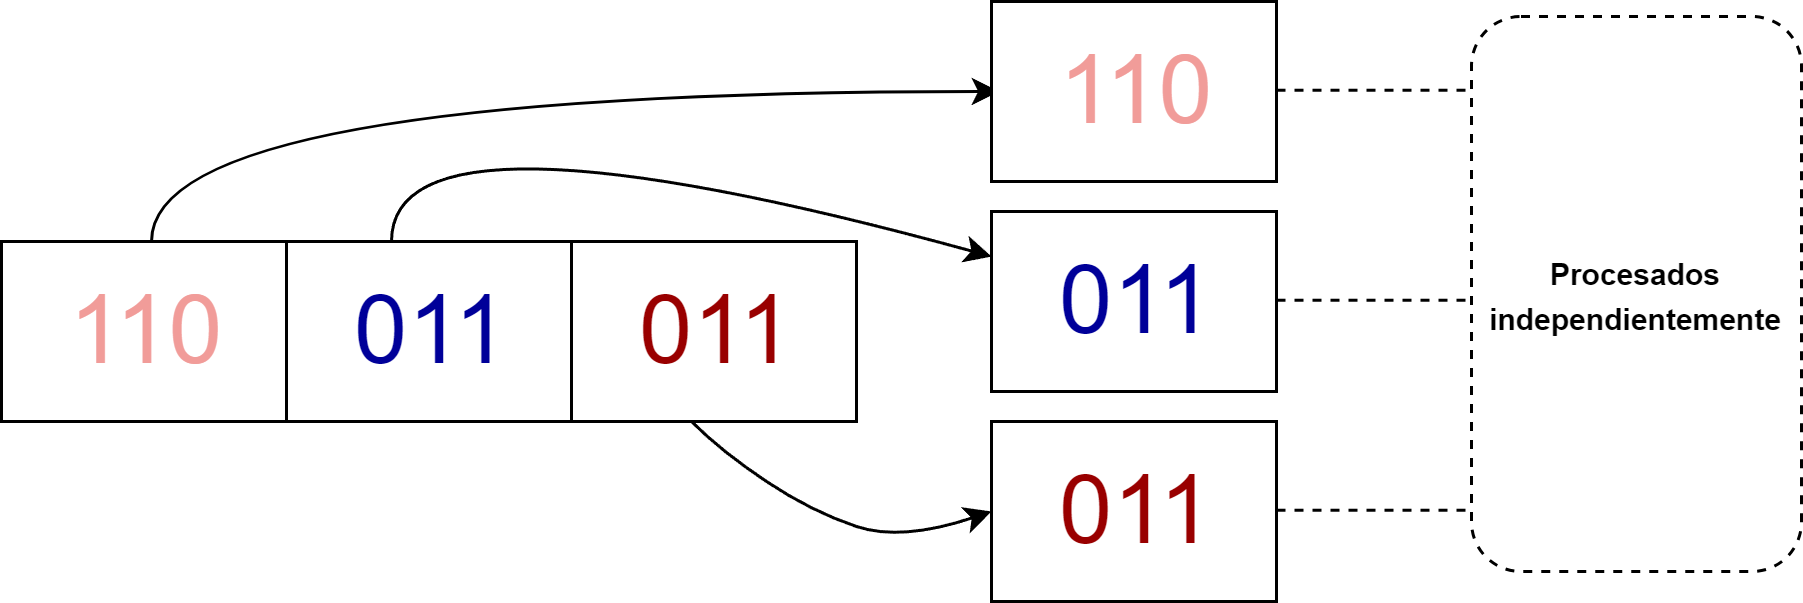
\includegraphics[width=0.7\textwidth]{img/codbloque.png}
    \caption{Funcionamiento códigos de bloque.}
    \label{fig:codbloque}
\end{figure}

Por otro lado, los códigos convolucionales utilizan un esquema de codificación que no depende únicamente del mensaje actual que se está transmitiendo, sino también de un cierto número de mensajes anteriores. Así, podríamos decir que, a diferencia de los códigos de bloque, un codificador de un código convolucional tiene "memoria".

\begin{figure}[h]
    \centering
    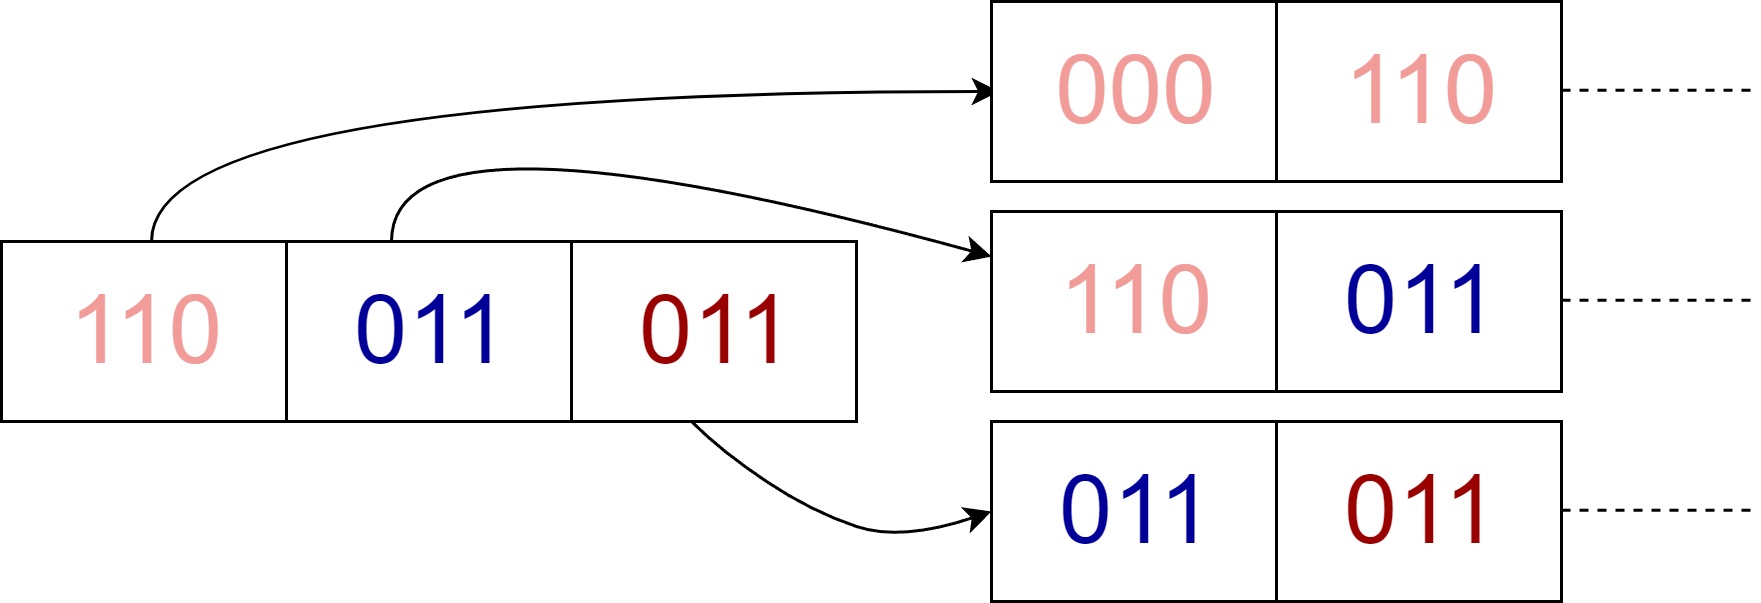
\includegraphics[width=0.7\textwidth]{img/codconvolucionales.png}
    \caption{Funcionamiento códigos convolucionales.}
    \label{fig:codconvolucional}
\end{figure}

Los códigos convolucionales fueron presentados por primera vez por Peter Elias  \cite{Elias1955} en 1955 como una alternativa a los códigos de bloque. El primer algoritmo de decodificación para estos códigos fue la decodificación secuencial sugerida por Wozencraft \cite{Wozencraft1957SequentialDF} en 1957 y posteriormente desarrollada por Fano, quien en 1963 propuso un método de decodificación muy ingenioso \cite{Fano1963}. Se desarrollaron muchos más algoritmos de decodificación para estos códigos, pero sin duda, el algoritmo de decodificación principal para estos códigos es el \emph{algoritmo de Viterbi}, el cual es un algoritmo de programación dinámica desarrollado por el ingeniero italiano A.J Viterbi \cite{Viterbi1967} en 1967.

Si bien estos códigos se desarrollaron en los años 50, no fue hasta 1970 cuando Forney \cite{Forney1970} desarrolló por primera vez una teoría algebraica sólida. No obstante, la teoría matemática existente para los códigos convolucionales no está tan desarrollada como lo está para los códigos de bloque. A lo largo de este capítulo presentaremos de varias formas los códigos convolucionales y estudiaremos cómo podemos codificar estos códigos mediante matrices generadoras.

Las principales fuentes para la redacción de este capítulo han sido \cite{Huffman_Pless_2010}, \cite{Forney1970}, \cite{Johannesson2015} , \cite{cccheide} y \cite{jl2020}.


\section{Matrices generadoras y codificación de códigos convolucionales}

Existen numerosas formas de definir los códigos convolucionales como veremos a lo largo del trabajo. Usualmente, los códigos convolucionales se han estudiado principalmente para el cuerpo $\F _2$, sin embargo, en los últimos años se han estudiado en ámbitos más generales, donde $\F$ es un cuerpo finito arbitrario.

Sea $\F$ un cuerpo finito y sea $t$\footnote{El símbolo $t$ representa el operador delay en los códigos convolucionales. En otras referencias bibliográficas (ver por ejemplo \cite{Huffman_Pless_2010}) se denota por $D$. } una indeterminada. Entonces, $\F[t]$ es el conjunto de todos los polinomios en la variable $t$ con coeficientes en $\F$. Este conjunto es un \emph{dominio de integridad} y, por tanto, podemos construir su \emph{cuerpo de fracciones}, al cual denotaremos $\F(t)$.

\begin{definicion}
    Un \emph{$(n,k)$-código convolucional} $\C$ es un subespacio $k$-dimensional de $\F(t)^n$.
\end{definicion}

Nótese que al ser $\F(t)$ un cuerpo infinito, $\C$ contendrá un número infinito de palabras código.

\begin{definicion}
    Sea $\C$ un $(n,k)$-código convolucional. El \emph{ratio} $R$ de $\C$ se define como $R = \frac{k}{n}$.
\end{definicion}

A diferencia de lo que ocurría con los códigos de bloque, no es usual considerar valores de $n$ y $k$ altos. Esto se debe a que la decodificación de códigos convolucionales es mucho más compleja.

\begin{definicion}
    Se dice que $G(t) \in \mathcal{M}_{k \times n}(\F(t))$ es una \emph{matriz generadora} de $\C$ si sus filas forman una base de $\C$.
\end{definicion}

Si $G(t)$ es una matriz generadora, entonces también lo será cualquier matriz obtenida como el producto de $G(t)$ y un elemento no nulo de $\F(t)$. Por tanto, si multiplicamos $G(t)$ por el mínimo común múltiplo de los denominadores de todas las entradas de la matriz, obtendremos una matriz generadora de $\C$ cuyas entradas están formadas por polinomios. Por tanto, cualquier código convolucional tiene una matriz generadora cuyas entradas son polinómicas. Dichas matrices reciben el nombre de \emph{matrices generadoras polinómicas} para $\C$.

\begin{ejemplo}
Sea $G_1(t) = \left[1 + t^2 \ \ \frac{1}{1 + t}\right]$ una matriz generadora de un $(2,1)$-código convolucional binario. Entonces la matriz $G_2(t) = (1+t)G_1(t) = \left[1 + t + t^2 + t^3 \ \ \ 1  \right]$ es una matriz generadora polinómica de $\C$.
\end{ejemplo}


Utilizaremos estas matrices para codificar mensajes. Partiremos de la suposición de que estos mensajes son \emph{finitos} \footnote{En teoría de códigos convolucionales es común trabajar con mensajes de longitud infinita, los cuales pueden representarse mediante series de Laurent formales en el cuerpo $\F((t)).$} y los representaremos mediante polinomios $x(t) = \sum_{i=0}^{L-1} x(i)t^i \in \F[t]^k$.

Vamos a describir el procedimiento de codificación para un $(n,k)$-código convolucional $\C$ utilizando una matriz generadora polinómica $G(t)$. Para enfatizar la conexión entre $G(t)$ y el proceso de codificación, a menudo nos referiremos a $G(t)$ como \emph{codificador}. Empezaremos suponiendo que $k = 1$, de esta manera, en cada momento $i = 0,1,\dots$ la entrada para el codificador $G(t)$ está formada por un único elemento $x(i) \in \F$. 

Supongamos que tenemos un flujo de entrada de $L$ elementos, cada uno de estos pertenecientes a $\F$. Estos elementos se representan como coeficientes de un polinomio $x(t)$, donde $t$ es una indeterminada que representa el operador delay. El polinomio se define como $x(t) = \sum_{i=0}^{L-1}x(i)t^i$, donde $x(i)$ es el símbolo $i$ del flujo de entrada. La codificación, al igual que con los códigos de bloque, se realiza mediante el producto $x(t)G(t) = c(t)$. La palabra código $c(t) = (c_1(t),\dots,c_n(t))$ tiene $n$ componentes, los cuales son polinomios \footnote{ Si suponemos que el codificador $G(t)$ no es polinómico, entonces $c(t)$ puede ser un elemento del cuerpo de fracciones $\F(t)^n$. } en $t$.

\begin{ejemplo}
Sea $\C$ un $(2,1)$-código convolucional binario y sea $G(t) = \left[ 1 + t + t^2 \ \ 1 + t^2 \right]$ su matriz generadora. Vamos a codificar el mensaje $\mathbf{m} = 110101$, cuya longitud es $L = 6$. Este mensaje corresponde al polinomio $x(t) =  \sum_{i=0}^{5}x(i)t^i = 1 + t + t^3 + t^5$. Lo codificamos utilizando la matriz generadora $G(t)$:
\begin{align*}
    c(t) &= x(t)G(t) \\
    &= (1 + t + t^3 + t^5)\left[ \begin{array}{cc}
    1 + t + t^2 & 1 + t^2 \\
    \end{array} \right] \\
    &= \left(1 + t^4 + t^6 + t^7, \ 1 + t + t^2 + t^7\right) \\
    &= (c_1(t), c_2(t)).
\end{align*}
Si observamos detenidamente las multiplicaciones y las sumas realizadas para calcular $c_1(t)$ y $c_2(t)$, podemos ver que tanto la memoria como el operador delay $t$ \emph{juega un papel crucial}. Puesto que $c_1(t) = x(t)(1 + t + t^2)$, en el momento $i$, observamos que $c_1(i) = x(i)(1 + t + t^2) = x(i) + x(i-1) + x(i-2)$. De manera análoga, se tiene que $c_2(i) = x(i) + x(i-2)$, estas ecuaciones reciben el nombre de \emph{ecuaciones del codificador}. Cada aparición de $t^j$ retrasa la entrada en $j$ unidades de tiempo. Diremos que la memoria del codificador es $M = 2$.
\end{ejemplo}

\begin{definicion}
Sea $\C$ un $(n,k)$-código convolucional y sea $G(t) \in \mathcal{M}_{k \times n}(F[t])$ una matriz generadora polinómica de este código. Sean $g_{ij}(t)$ los elementos de $G(t)$. Se define la \emph{memoria $M$ de $G(t)$} como el mayor grado de cualquier elemento de $G(t)$, es decir,
$$ M = \max_{\substack{1 \leq i \leq k \\ 1 \leq j \leq n}} \left\{ \gr(g_{ij}(t)) \right\}.$$
\end{definicion}

Algo a tener en cuenta es que la memoria \emph{depende exclusivamente del codificador} $G(t)$ y no del código $\C$. Recordemos que si multiplicamos la matriz $G(t)$ por cualquier elemento no nulo de $\F[t]$, seguirá siendo una matriz generadora para $\C$, sin embargo, su memoria puede cambiar.

Podemos generalizar el proceso de codificación anterior a un $k$ arbitrario. En esta ocasión, la entrada en el instante $i = 0,1,\dots$ está formada por los elementos $x_j(i) \in \F, \ j \in \{1,\dots,k\}$, los cuales forman el mensaje $\mathbf{x}(i) = (x_1(i),\dots,x_k(i))$. Al igual que antes, podemos reescribir cada $x_j$ como un polinomio en la indeterminada $t$. De esta forma, la entrada resultante $\textbf{x}(t)$ será un vector de $k$ polinomios. La palabra código se calcula, de nuevo, como $\mathbf{x}(t)G(t) = \mathbf{c}(t) = (c_1(t),c_2(t),\cdots,c_n(t))$. Veamos un ejemplo.

\begin{ejemplo}
Sea $\C$ un $(4,2)$-código convolucional binario y sea $$G(t) = \left[ \begin{array}{cccc}
    1 & 1 + t + t^2 & 1 + t^2 & 1 + t \\
    0 & 1 + t & t & 1 \\
    \end{array} \right]$$ 
una matriz generadora. Vamos a codificar el mensaje $\mathbf{m} = (11010,10111)$, el cual corresponde al par polinómico $\mathbf{x}(t) = (1 + t + t^3,1 + t^2 + t^3 + t^4)$. Lo codificamos mediante la matriz generadora $G(t)$:

\begin{align*}
    \mathbf{x}(t)G(t) &= (1 + t + t^3, 1 + t^2 + t^3 + t^4) \left[ \begin{array}{cccc}
        1 & 1 + t + t^2 & 1 + t^2 & 1 + t \\
        0 & 1 + t & t & 1 \\
    \end{array} \right] \\
    &= (1 + t + t^3, 1 + t^2 + t^4, 1 + t^2 + t^3 + t^4, 0 ) = \mathbf{c}(t).
    \end{align*}

Como el máximo grado de los elementos de $G(t)$ es $2$, sabemos que su memoria $M$ será también $2$. Podemos también calcular las ecuaciones del codificador $G(t)$ de manera análoga al caso $k=1$.

\[
\left\{
\begin{aligned}
    c_1(i) &= x_1(i), \\
    c_2(i) &= x_1(i) + x_1(i-1) + x_1(i-2) + x_2(i) + x_2(i-1),   \\
    c_3(i) &= x_1(i) + x_1(i-2) + x_2(i-1),\\
    c_4(i) &= x_1(i) + x_1(i-1) + x_2(i).\\
\end{aligned}
\right.
\]
\end{ejemplo}

Hemos visto como se puede codificar un mensaje mediante códigos convolucionales de forma matemática mediante la matriz generadora $G(t)$. Sin embargo, es interesante estudiar cómo podríamos construir un \emph{codificador físico} \footnote{Nos centraremos en el caso en el que el cuerpo es $\F_2$ pues, al tratarse de 1's y 0's, su implementación es más sencilla. } mediante registros de desplazamiento. Para codificar códigos convolucionales podemos usar registros de desplazamiento con retroalimentación lineal, un tipo particular de registros de desplazamiento en el que la entrada es un bit proveniente de aplicar una función de transformación lineal a un estado anterior. Los componentes principales de estos registros son los elementos de delay (también llamados flip-flops) y los sumadores binarios mostrados en la Figura \ref{fig:encoder}.

\begin{figure}[h]
    \centering
    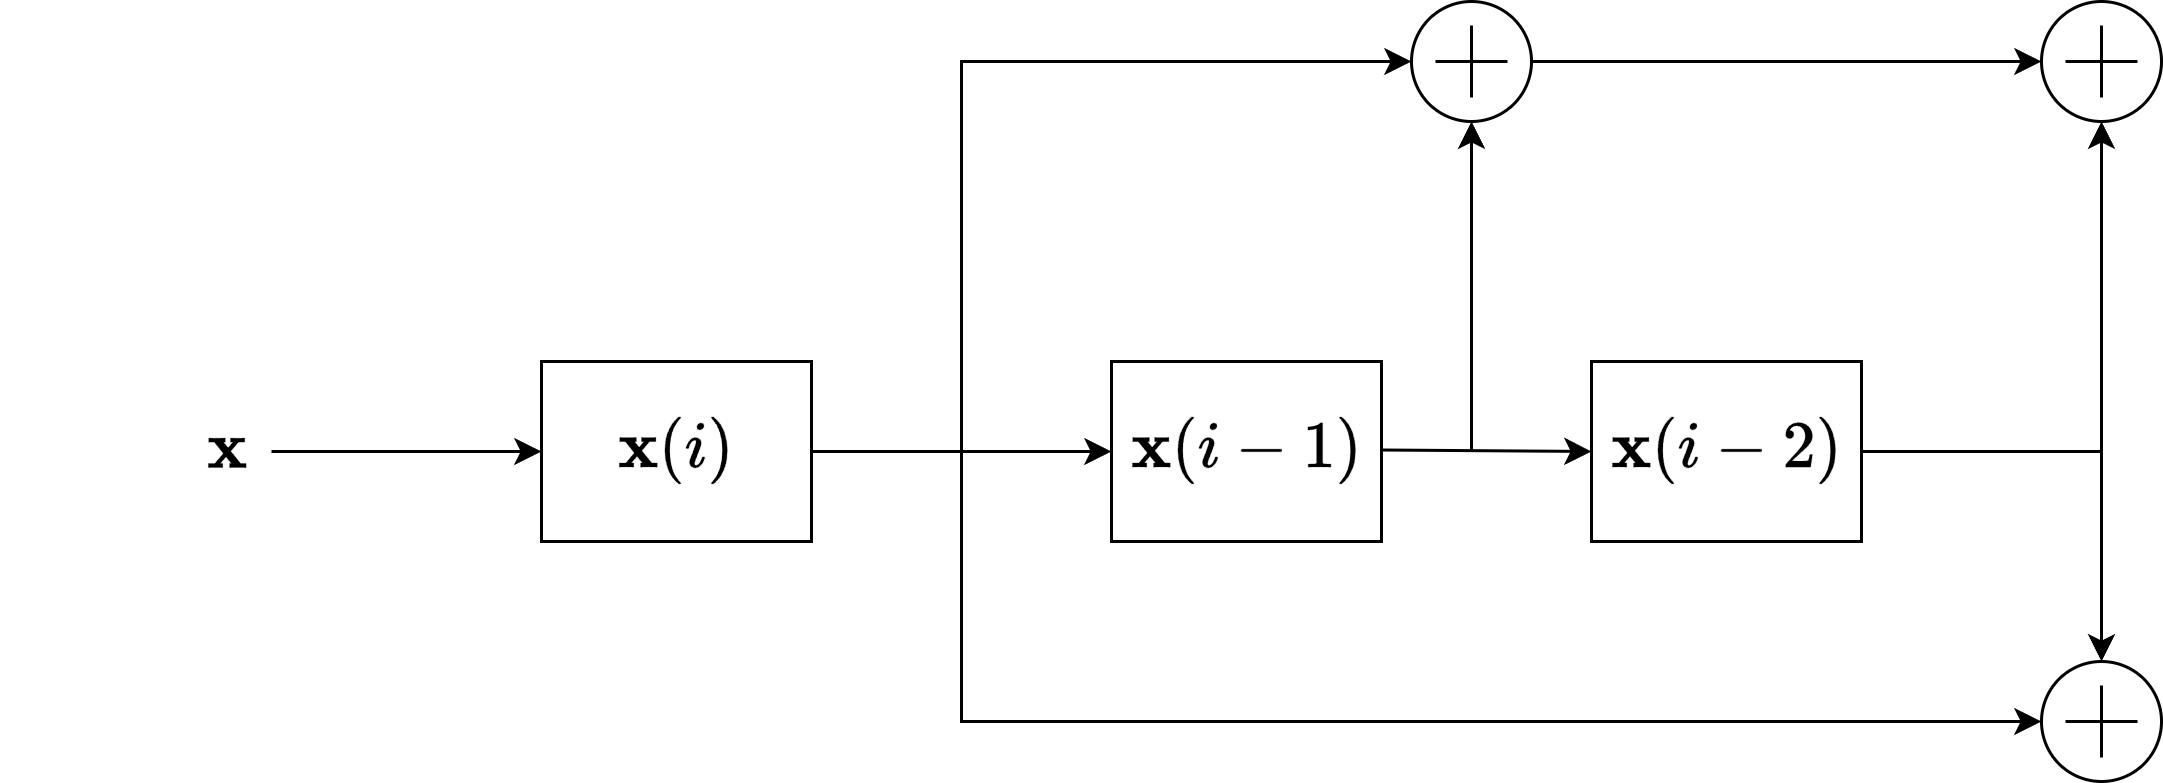
\includegraphics[width=0.8\textwidth]{img/codfisico.png}
    \caption{Codificador físico para $G(t) = \left[ 1 + t + t^2 \ \ 1 + t^2 \right]$.}
    \label{fig:encoder}
\end{figure}

\section{Matrices generadoras canónicas}

Hemos visto que un código convolucional $\C$ puede tener varias matrices generadoras, incluyendo matrices cuyas entradas son funciones racionales. Hasta ahora, nos hemos enfocado en las matrices generadoras polinómicas, pero en esta sección, definiremos una subclase de las matrices generadora polinómicas: las \emph{matrices generadoras canónicas}.


Empecemos con unas definiciones importantes. Sea $G(t) = [g_{ij}(t)]$ una matriz polinómica de dimensión $k\times n$.

\begin{definicion}
 Se define \emph{el grado $m_i$ de la $i$-ésima fila de $G(t)$}  como el máximo grado de cualquier elemento de la fila $i$, para $i \in \{1,\dots,k\}$. Es decir,
$$m_i = \max_{1 \leq j \leq n} \gr(g_{ij}(t)).$$
\end{definicion}

\begin{definicion}
Se define el \emph{grado externo} de $G(t)$, denotado extdeg($G(t)$), como la suma de los grados de las $k$ filas de $G(t)$. Es decir,
$$\extdeg(G(t)) = \sum_{i=1}^{k} m_i.$$
\end{definicion}

\begin{ejemplo}
\label{ej:cc}
Sea $G_1(t) = \left[1 + t + t^2 \ \ 1 \right]$ una matriz generadora de un $(2,1)$-código convolucional binario. Como solo tiene una fila, su grado externo y el grado de la fila $1$ coinciden, y este es $2$.


Sea $G_2(t) = \left[ \begin{array}{cccc}
    1 & 1 + t + t^2 & 1 + t^2 & 1 + t \\
    0 & 1 + t & t & 1 \\
\end{array} \right]$ una matriz generadora de un $(4,2)$-código convolucional binario. Entonces $m_1 = 2$, $m_2 = 1$ y, por tanto, extdeg($G(t)$) $ = m_1 + m_2 = 3$. 
\end{ejemplo}

\begin{definicion}
Una \emph{matriz generadora canónica} para un código convolucional $\C$ es una matriz generadora polinómica cuyo grado externo es el mínimo posible entre todas las posibles matrices generadoras polinómicas para $\C$.
\end{definicion}


Por definición, todos los códigos convolucionales cuentan con una matriz generadora canónica. Este grado externo mínimo recibe el nombre de \emph{grado} del código $\C$.

Nótese que la matriz generadora canónica no es única (salvo el caso en el que el cuerpo sea $\F_2$), ya que podemos multiplicar esta matriz por cualquier elemento de $\F$ y seguiría conservando el grado externo.

\begin{ejemplo}
\label{ej:mgc}
Vamos a demostrar que la matriz generadora $G_1(t)$ del ejemplo \ref{ej:cc} es canónica para el $(2,1)$-código convolucional binario $\C$. En este caso, el grado externo de cualquier matriz generadora polinómica de $\C$ es el grado máximo de sus entradas (pues solo tiene una fila). Cualquier otra matriz generadora $G_1'(t)$ de $\C$ puede obtenerse de $G_1(t)$ multiplicando esta por un elemento de $\F(t)$, es decir, por una expresión del tipo $p(t)/q(t)$, donde $p(t),q(t) \in \F[t]$ (con $q(t) \neq 0$). Supondremos que $p(t)$ y $q(t)$ son polinomios coprimos (en caso contrario solo habría que simplificar). De esta forma, $G_1'(t) = \frac{p(t)}{q(t)}G_1(t)$. 

Como las matrices generadoras canónicas son polinómicas, $q(t)$ debe dividir a los dos elementos de $G_1(t)$ y como el segundo elemento es $1$, $q(t) = 1$. Por tanto, $G_1'(t) = p(t)G_1(t)$. De esta manera, para que no aumente el grado debe ocurrir que $\gr(p(t)) = 0$, o lo que es lo mismo, $p(t) \in \F$. Esto demuestra que $G_1(t)$ es una matriz generadora canónica.
\end{ejemplo}

El razonamiento del Ejemplo \ref{ej:mgc} nos dice que si $\C$ es un $(n,1)$-código convolucional, una matriz generadora polinómica $G(t)$ será canónica si y solo si el máximo común divisor de sus entradas es $1$. Esto no es tan fácil cuando $k > 1$. A lo largo de esta sección buscaremos una condición \emph{necesaria y suficiente} para que una matriz generadora polinómica sea una matriz generadora canónica de un $(n,k)$-código convolucional. Antes de demostrarlo vamos a introducir los siguientes conceptos.

\begin{definicion}\label{def:complejidad}
Sea $G(t)$ una matriz polinómica de dimensión $k\times n$, con $k \leq n$. El \emph{grado interno} de $G(t)$, denotado como intdeg($G(t)$), es el máximo grado de todos los menores \footnote{Un menor de dimensión $k \times k$ de una matriz $M$ de dimensión $k \times n$, $k \leq n$ es el determinante de una matriz formada por $k$ columnas de $M$. La matriz $M$ tiene $\binom{n}{k}$ menores.} de $G(t)$ de dimensión $k \times k$. También se suele llamar \emph{complejidad del código}. Un código de complejidad $0$ es un código de bloque.
\end{definicion}

\begin{definicion}
Se dice que una matriz generadora polinómica de un código convolucional $\C$ es \emph{básica} si su grado interno es mínimo.
\end{definicion}

\begin{definicion}
Una matriz polinómica $G(t)$ es \emph{reducida} si entre todas las matrices de la forma $U(t)G(t)$, donde $U(t)$ es una matriz unimodular \footnote{Una matriz $U$ de dimensión $k \times k$ es \emph{unimodular} si su determinante es $1$.} de dimensión $k \times k$, $G(t)$ tiene el grado externo más pequeño.
\end{definicion}

En \cite{mceliece1998}, McEliece dio seis formulaciones equivalentes para que una matriz sea básica y tres para que sea reducida. Presentaremos algunas de estas equivalencias y omitiremos las demostraciones. Estas pueden ser encontradas en \cite[Apéndice A]{mceliece1998}.

\begin{teorema}
\label{th:cc1}
Sea $G$ una matriz generadora polinómica de un $(n,k)$-código convolucional. Equivalen las siguientes afirmaciones:
\begin{itemize}
    \item[(i)] La matriz $G$ es básica.
    \item[(ii)] El máximo común divisor de los menores $k \times k$ de $G(t)$ es $1$.
    \item[(iii)] Existe una matriz $K(t) \in \mathcal{M}_{n \times k}(\F[t])$ tal que $G(t)K(t) = I_k$.
    \item[(iv)] Si $\mathbf{c}(t) \in \F[t]^n$ y $\mathbf{c}(t) = \mathbf{x}(t)G(t)$, entonces $\mathbf{x}(t) \in \F[t]^k$.
\end{itemize}
\end{teorema}

Recordemos que la matriz $K(t)$ en (iii) es la inversa por la derecha de $G(t)$. La equivalencia (iii) del Teorema \ref{th:cc1} establece que si $G(t)$ es un codificador básico, entonces siempre que la entrada sea polinomial, también lo será la salida. La prueba de que (iii) implica (iv) es simple. Si (iii) se verifica y $\mathbf{c}(t) = \mathbf{x}(t)G(t)$, entonces $\mathbf{x}(t) = \mathbf{x}(t)I_k = \mathbf{x}(t)G(t)K(t) = \mathbf{c}(t)K(t)$. Como $c(t)$ y $K(t)$ solo tienen entradas polinomiales, también las tendrá $\mathbf{x}(t)$.

\begin{definicion}
El \emph{grado} de un vector $\mathbf{v}(t) \in \F[t]^n$ es el mayor grado de cualquiera de sus componentes. \footnote{Nótese que esta definición es consistente con la definción que hemos dado antes del grado de una matriz.}
\end{definicion}

\begin{teorema}
\label{th:aux}
Sea $G(t) \in \mathcal{M}_{k \times n}(\F[t])$ y sea $g_i(t)$ la i-ésima fila de $G(t)$. Equivalen las siguientes afirmaciones:
\begin{itemize}
    \item[(i)] La matriz $G$ es reducida.
    \item[(ii)] $\intdeg(G(t)) = \extdeg(G(t))$.
    \item[(iii)] Para cualquier $\mathbf{x}(t) = (x_1(t),\dots,x_k(t)) \in \F[t]^k$, se verifica 
    $$\gr(\mathbf{x}(t)G(t)) = \max_{i \leq i \leq k} \{\gr(x_i(t)) + \gr(g_i(t))\}.$$  
\end{itemize}
\end{teorema}

Nuestro objetivo será probar que una matriz generadora polinómica de un $(n,k)$-código convolucional es canónica si y solo si es básica y reducida. Para ello, necesitaremos el siguiente lema.

\begin{lema}
\label{lm:cc1}
Sea $G(t) \in \mathcal{M}_{k \times n}(\F[t])$ una matriz generadora polinómica de un código convolucional $\C$, $ k \leq n$. Sea $N(t)$ una matriz no singular de dimensión $k \times k$ con entradas en $\F[t]$. Se verifican las siguientes afirmaciones:
\begin{itemize}
    \item[(i)] $\intdeg(N(t)G(t)) = \intdeg(G(t)) + \deg(\det(N(t)))$.
    \item[(ii)] $\intdeg(G(t)) \leq \intdeg(N(t)G(t))$. La igualdad se verifica si y solo si $N$ es unimodular.
    \item[(iii)] $\intdeg(G(t)) \leq \extdeg(G(t))$.  
\end{itemize}
\end{lema}

\begin{proof}
Para probar (i) observamos que las submatrices de dimensión $k \times k$ de $N(t)G(t)$ son precisamente las submatrices $k \times k$ de $G(t)$ multiplicadas por $N(t)$ a la izquierda. Por tanto, los menores $k \times k$ de $N(t)G(t)$ son exactamente los menores $k \times k$ de $G(t)$ multiplicados cada uno por $\det(N(t))$. Lo que prueba (i). 

La parte (ii) se deduce de (i). 

Para (iii), supongamos que el grado de la $i$-ésima fila de $G(t)$ es $m_i$. Entonces, extdeg($G(t)$) $m_1 + \cdots + m_k$. Cualquier menor $k \times k$ de $G(t)$ es una suma de productos de entradas de $G(t)$, con un factor de cada fila en cada producto. Por tanto, el mayor grado posible del producto es  $m_1 + \cdots + m_k$, lo que prueba (iii).  
\end{proof}

Con este resultado, podemos probar el teorema principal de esta sección, el cual caracteriza las matrices canónicas de un código convolucional.

\begin{teorema}
Una matriz generadora polinómica de un $(n,k)$-código convolucional $\C$ es canónica si y solo si es básica y reducida.
\end{teorema}

\begin{proof} \phantom{}

\boxed{\Rightarrow}

Sea $G$ una matriz generadora canónica para $\C$. Sea $d_0$ el grado interno de las matrices generadoras básicas, que recordemos que es mínimo. Elegimos de entre todas las matrices generadoras básicas, una matriz $G_0(t)$ con grado externo mínimo.

Sea $U(t)$ una matriz unimodular de dimensión $k \times k$. Entonces utilizando el Lema \ref{lm:cc1}, $$U(t)G_0(t) = \intdeg(G_0(t)) = d_0.$$

Por definición de $G_0(t)$, $\extdeg(U(t)G_0(t)) \geq \extdeg(G_0(t))$ (ya que $U(t)G_0(t)$ genera $\C$), lo que implica que $G_0(t)$ es reducida. Teniendo en cuenta que $G_0(t)$ tiene el grado interno más pequeño de entre todas las matrices generadoras polinómicas de $\C$, $\intdeg(G_0(t)) \leq \intdeg(G(t))$. Pero intdeg($G(t)$) $\leq$ extdeg($G(t)$) por el Lema \ref{lm:cc1} y extdeg($G(t)$) $\leq$ extdeg($G_0$) por definición, ya que $G(t)$ es canónica. Por tanto,

\begin{equation}
\label{ec:1}
\intdeg(G_0(t)) \leq \intdeg(G(t)) \leq \extdeg(G(t)) \leq \extdeg(G_0(t)).
\end{equation}

Como $G_0(t)$ es reducida, $\intdeg(G_0(t)) = \extdeg(G_0(t))$ por el Teorema \ref{th:aux}. Y, por tanto, se da la igualdad en \eqref{ec:1}. 

De esta manera, $\intdeg(G(t)) = \intdeg(G_0(t)) = d_0$ probando que $G(t)$ tiene también grado interno mínimo entre todas las matrices generadoras polinómicas de $\C$, lo que implica que es básica. Como $\intdeg(G(t)) = \extdeg(G(t))$, obtenemos que $G(t)$ también es reducida.

\boxed{\Leftarrow}

Supongamos ahora que $G(t)$ es una matriz generadora polinómica de $\C$ reducida y básica. Sea $G_0(t)$ otra matriz generadora polinómica de $\C$. Por el Lema \ref{lm:cc1}, $\extdeg(G_0(t)) \geq \intdeg(G_0(t))$. Como $G(t)$ es básica, intdeg($G_0(t)$) $\geq$ intdeg($G(t)$). Y como también es reducida, $intdeg(G(t)) = \extdeg(G(t))$. Combinando estas desigualdades, llegamos a que extdeg($G_0(t)$) $\geq$ extdeg($G(t)$). Lo que implica que $G(t)$ es canónica, al ser $G_0(t)$ una matriz generadora polinómica arbitraria.
\end{proof}

\section{Códigos convolucionales y módulos}

Hasta ahora, hemos visto a los códigos convolucionales como subespacios $k$-dimensionales del cuerpo de fracciones $\F(t)^n$. Sin embargo, existen \emph{varias definiciones de códigos convolucionales} y algunos autores han utilizado la teoría de módulos para describir los códigos convolucionales. En esta sección vamos a trabajar con algunos conceptos referentes a los códigos convolucionales usando módulos.


\begin{definicion} \label{def:ccm}
Un \emph{$(n,k)$-código convolucional} es un sumando directo $\C$ del módulo $\F[t]^n$ de rango $k$.
\end{definicion}

En principio, parecen dos formas totalmente distintas de ver los códigos convolucionales. No obstante, ambas formas están íntimamente relacionadas, como nos muestra este resultado, mencionado en \cite{gomez2017sugiyama}.

\begin{proposicion}\label{prop:relacion}
Sea $k \leq n$. La aplicación $D \rightarrow D \cap \F[t]^n$ establece una biyección entre el conjunto de los subespacios $k$-dimensionales de $\F(t)^n$ y el conjunto de todos los $\F[t]$-submódulos de $\F[t]^n$ con rango $k$ que son sumandos directos de $\F[t]^n$.
\end{proposicion}

Esta proposición es un resultado de teoría de módulos y es un refinamiento del Teorema 3 de \cite{Forney1970}.

\begin{definicion}
Una \emph{matriz generadora o codificadora} es cualquier matriz $G(t) \in \mathcal{M}_{k \times n}(\F[t])$ de rango $k$ que genere un código convolucional $\C$. Por tanto, 
$$ \C = Im(G(t)) = \{u(t)G(t) \ | \ u(t) \in \F[t]^k\} $$ y el vector $u(t)G(t) \in \F[t]^n$ es la palabra código asociada al mensaje $u(t) \in \F[t]^k$.
\end{definicion}

Observamos que las matrices generadoras de los códigos convolucionales vistos como sumandos directos del módulo $\F[t]^n$ son muy parecidas a las que definimos al principio de este capítulo. La única diferencia es que mientras que en las anteriores permitíamos coeficientes racionales del cuerpo de fracciones $\F(t)$, en estas matrices solo permitimos coeficientes polinómicos del DIP $\F[t]$. Sin embargo, recordemos que cualquier matriz generadora con coeficientes en $\F(t)$ se puede transformar en otra matriz que genere el mismo código con coeficientes en $\F[t]$ multiplicando por el mínimo común múltiplo de los denominadores de los coeficientes.


\begin{definicion}
Una \emph{matriz de paridad de un código convolucional} $\C$ es cualquier matriz $H(t) \in \mathcal{M}_{n \times (n-k)}(\F[t])$ que satisfaga $$\C = \ker H(t) =  \{v \in \F^n \ | \ v(t)H(t) = 0\}.$$
\end{definicion}

\begin{definicion}
Sea $V$ un submódulo de $\F[t]^n$. Entonces 
\begin{itemize}
    \item[(i)] Se dice que $V$ es \emph{no catastrófico} si \eqref{eq:modu1} se satisface para todo $v \in \F[t]^n$ y todo $\lambda \in \F[t]\backslash t\F[t]$.
    \item[(ii)] Se dice que $V$ es libre de delay si \eqref{eq:modu1} se satisface para todo $v \in \F[t]^n$ y $\lambda = t$. 
\end{itemize}
\end{definicion}

Un submódulo $V$ no catastrófico y libre de delay es, por definición, \emph{un código convolucional}, en base a la Proposición \ref{prop:cc3}, que nos asegura que $V$ es un sumando directo de $\F[t]^n$.

\section{Distancias en códigos convolucionales}\label{sec:distancias}

Al igual que los códigos de bloque, la distancia en los códigos convolucionales es una medida muy importante, pues nos permite evaluar la capacidad de un código para detectar y corregir los errores que se han producido en la transmisión. En lo que sigue, consideraremos a $\C$ un sumando directo del módulo libre $\F[t]^n$ de rango $k$.

Para los códigos de bloque utilizábamos la distancia de Hamming. Dados dos mensajes, $\mathbf{x,y} \in \F^n$ su distancia de Hamming es el número de coordenadas en las que difieren $\mathbf{x}$ e $\mathbf{y}$. Vimos que también se podía definir utilizando el peso de Hamming, que consistía en el número de coordenadas no nulas de una palabra $\mathbf{x} \in \F^n$. Así, $d(x,y) = wt(x - y)$.

Podemos extender esta definición a los códigos convolucionales de la siguiente forma.

\begin{definicion}
Sea $c(t) = \sum_{i=0}^{\gr(c(t))} c_it^i\in \F[t]^n$. Definimos su peso de Hamming como $$wt(c(t)) = \sum_{i=0}^{\gr(c(t))}wt(c_i).$$
\end{definicion}

\begin{definicion}
Sean $c_1(t),c_2(t) \in \F[t]^n$. Definimos su distancia de Hamming como 
$$d(c_1(t),c_2(t)) = wt(c_1(t) - c_2(t)).$$
\end{definicion}

\begin{definicion}\label{def:libre}
La \emph{distancia libre} de un código convolucional $\C$ es la mínima distancia entre dos palabras código distintas. Es decir,
$$d_{\text{free}}(\C) = \min_{c_1(t),c_2(t) \in \C} \{d(c_1(t),c_2(t)) \ | \ c_1(t) \neq c_2(t)\}.$$
\end{definicion}

Durante la transmisión en un canal $q$-ario simétrico \footnote{Donde $q$ es el número de elementos del cuerpo finito $\F$.} se pueden producir varios errores. No obstante, mediante la distancia libre, podemos determinar el número de errores que podemos detectar y corregir.

\begin{teorema}
Sea $\C$ un código convolucional con distancia libre $d$. Entonces, $\C$ puede detectar $d - 1$ errores y puede corregir hasta $$ t = \left\lfloor \frac{d-1}{2} \right\rfloor.$$
\end{teorema}

\begin{proof}
Análoga a la realizada para los códigos de bloque en \ref{th:errores}.
\end{proof}

\begin{lema}
La distancia libre de un código convolucional $\C$ se puede calcular como

$$d_{\text{free}} = \min_{c(t) \in \C} \{wt(c(t)) \ | \ c(t) \neq 0\}$$
\end{lema}

\begin{proof}
    Demostración análoga a la realizada en \ref{th:wp}.
\end{proof}

Además de la distancia libre, los códigos convolucionales también poseen otra noción de distancia.

\begin{definicion}
Sea $ x(t) \in \F[t]^n$ con $\gr(c(t)) = \gamma$, entonces $x(t) = x_0 + + x_1t +  \cdots + x_{\gamma}t^{\gamma}$ con $x_i \in \F^n$ para $t \in \{0,\dots,\gamma\}$ y $c_i = \mathbf{0}$ para $i \geq \gamma + 1$. Definimos la truncación $j$-ésima de $c(t)$ como $$c_{[0,j]}(t) = c_0 + c_1t + \cdots + c_jt^j.$$
\end{definicion}

\begin{definicion}
Para $j \in \N_0$, la distancia de la $j$-ésima de un código convolucional $\C$ se define como
$$d_j^c(\C) := \min_{c(t) \in \C} \{wt(c_{[0,j]}(t)) \ | \ c_0 \neq \mathbf{0}\}.$$
\end{definicion}

Al igual que con los códigos de bloque, existen límites superiores para las distancias de los códigos convolucionales.

Recordemos que para los códigos de bloque, disponíamos de la cota de Singleton \ref{th:cotaS}. En el caso de los códigos convolucionales, también existe un límite superior para la distancia libre.

Sea $G(t)$ una matriz generadora de un código convolucional $\C$. Esta matriz podemos separarla en una suma finita de matrices de distintos grados, denotaremos por $G_{\infty} \in M_{k \times n}(\F[t])$ a la matriz de mayor grado de $G(t)$. En general, $G_{\infty}$ no tiene rango $k$.

Sin embargo, cada módulo $\C$ de rango $k$  tiene una matriz generadora $G'(t)$ tal que los grados de las filas decrecen y $G'_{\infty}$ tiene rango $k$ \cite{Rosenthal1999}. Además, en este caso, $\intdeg(G'(t))  = \sum_{i=1}^{k} v_i$, donde $v_i$ es el grado de la i-ésima fila de $G(t)$. Si una matriz $G(t)$ cumple estas condiciones, diremos que está en \emph{forma propia}. Los índices ordenados $v_1 \geq \cdots \geq v_k$ son invariantes del código convolucional y se denominan \emph{índices de Kronecker} del código convolucional $\C$. 


Los siguientes resultados se pueden encontrar en \cite{Rosenthal1999}. 

El siguiente lema será fundamental para encontrar una cota de $d_{\text{free}}$.
\begin{lema}
Sea $\C$ un $(n,k)$-código convolucional, sea $\delta$ su grado interno y sea $G(t)$ una matriz generadora polinómica en forma propia. Sea $\ell$ el número de índices $v_i$ entre los índices ordenados $v_1 \geq \cdots \geq v_k$ tales que $v_i = v_k$. Entonces la distancia libre satisface 
\begin{equation}\label{eq:lemad}
d_{\text{free}} \leq n(v_k + 1) - \ell + 1.
\end{equation}
\end{lema}

Utilizando el lema anterior, es fácil probar el siguiente teorema, el cual nos da una cota de la distancia libre de un código convolucional.

\begin{teorema}[Cota de Singleton Generalizada]\label{th:singleton2}
Sea $\C$ un $(n,k)$-código convolucional y sea $\delta$ su grado interno. Entonces, \begin{equation} \label{eq:cotaSC} d_{free}(\C) \leq (n-k)\left(\left\lfloor \frac{\delta}{k}\right\rfloor + 1\right) + \delta + 1.\end{equation}
\end{teorema}

\begin{proof}
\phantom{\\}
La cota \eqref{eq:lemad} es mayor conforme aumenta $v_k$ y disminuye $\ell$. El valor más alto posible de $v_k$ es $\left\lfloor \frac{\delta}{k} \right\rfloor$ ya que recordemos que $v_k$ es el grado más pequeño posible de una fila y como $G(t)$ está en forma propia, $\delta = \sum_{i=1}^{k} v_i$. Un valor de $v_k$ mayor significaría que $\sum_{i=1}^{k} v_i \geq \delta$ lo que es imposible. 

Partimos de que $v_{k-\ell + 1} = v_{k-\ell + 2} = \cdots = v_{k} = \left\lfloor \frac{\delta}{k} \right\rfloor$. Sabemos también que $ \delta = \sum_{i=1}^{k} v_i = \sum_{i=1}^{k-\ell} v_i + \ell  \left\lfloor \frac{\delta}{k} \right\rfloor$. Debemos minimizar los $v_i$, pero deben ser mayores que $\left\lfloor \frac{\delta}{k} \right\rfloor$. Por tanto, los valores óptimos que minimizan $\ell$ son $v_1 = v_2 = \cdots = v_{k-\ell} = \left\lfloor \frac{\delta}{k} \right\rfloor + 1$, $v_{k-\ell + 1} = v_{k-\ell + 2} = \cdots = v_{k} = \left\lfloor \frac{\delta}{k} \right\rfloor$. De esta forma, 

$$ \delta = \sum_{i=1}^{k} v_i = (k - \ell)(\left\lfloor \frac{\delta}{k} \right\rfloor + 1) + \ell\left\lfloor \frac{\delta}{k} \right\rfloor = k\left\lfloor \frac{\delta}{k} \right\rfloor + k - \ell \Rightarrow \ell = k - \delta + k\left\lfloor \frac{\delta}{k} \right\rfloor.$$

Sustituyendo este valor de $\ell$ en la cota \eqref{eq:lemad} obtenemos la cota \eqref{eq:cotaSC}. 



\end{proof}





\endinput
% !TeX root = ../libro.tex
% !TeX encoding = utf8

%\setchapterpreamble[c][0.75\linewidth]{%
%	\sffamily
%  Breve resumen del capítulo. TODO
%	\par\bigskip
%}

\chapter{Códigos Convolucionales Cíclicos}\label{ch:cuarto-capitulo}

En el capítulo anterior hemos estudiado los códigos convolucionales. Al igual que con los códigos de bloque, podríamos pensar en definir una nueva subclase de estos códigos que cumpla una propiedad de ciclicidad. No obstante, como ya se comentó, la teoría matemática de los códigos convolucionales está mucho menos desarrollada que la de los códigos de bloque y esta brecha es aún mayor para la teoría matemática de los códigos cíclicos convolucionales.

En 1976, Piret \cite{Piret}  estableció una base matemática  para la teoría de códigos cíclicos convolucionales (CCC). Uno de sus descubrimientos principales fue que la ciclicidad clásica, tal y como la conocemos para los códigos de bloque, no funciona bien para los códigos convolucionales. Sin embargo, descubrió que trabajando en álgebras no conmutativas sí que existía una sorprendente analogía con los códigos cíclicos de bloque, ya que se podían definir los CCCs como ideales principales de un anillo no conmutativo.

Pocos años después, Roos \cite{Roos} observó que estas álgebras no conmutativas que usó Piret eran un caso particular de las extensiones de Ore, definidas por Ore en 1933 \cite{ore1933}. De esta forma, Roos consideró álgebras más generales para la construcción de los CCCs. Sin embargo, estas ideas no fueron profundamente desarrolladas durante esos años, quizás porque los investigadores no estaban muy familiarizados con los polinomios de Ore y su manipulación. No fue hasta 2004 que Fluesing-Luerssen y Schmale \cite{GL2004} desarrollaron un estudio detallado de (como ellos lo llamaron) los $\sigma$-CCCs, en el que se trabaja con la noción de código convolucional $\C$ como un sumando directo del módulo libre $\F[t]^n$.

En este capítulo, vamos a definir el anillo de polinomios de Ore, los cuales nos permitirán construir unos nuevos tipos de CCCs, llamados códigos convolucionales cíclicos sesgados (SCCC), que a diferencia de los $\sigma$-CCCs, se considera a los códigos convolucionales $\C$ como un subespacio vectorial $k$-dimensional del cuerpo de fracciones $\F(t)^n$. Esto nos permitirá utilizar herramientas desarrolladas para polinomios de Ore que solo están disponibles cuando se trabaja con anillos de división.

Las principales referencias bibliográficas para la redacción de este capítulo han sido \cite{gluesingluerssen2019skewpolynomial} y \cite{jacobson1996} para los anillos de polinomios sesgados, además de \cite{cccheide}, \cite{SCCC} y \cite{gomez2017sugiyama} para los SCCC.

\section{Anillos de polinomios sesgados}
En esta sección se van a introducir los anillos de polinomios sesgados, los cuales son esenciales para definir los códigos convolucionales cíclicos sesgados. Estos polinomios, también conocidos como polinomios de Ore, fueron estudiados por Oystein Ore en \cite{ore1933}. La principal particularidad de estos era que sus coeficientes podían pertenecer a un anillo de división arbitrario, conmutativo o no conmutativo, con la restricción de que el grado del producto de dos polinomios sea igual a la suma de los grados de los factores

\begin{definicion}
    Sea $\mathcal{R}$ un anillo, $\sigma$ un endomorfismo de anillos de $\mathcal{R}$ y $\delta$ una $\sigma$-derivación por la izquierda de $\mathcal{R}$, es decir, $\delta$ es aditivo y para $a,b \in \mathcal{R}$ se verifica que 
    $$ \delta(ab) = \sigma(a)\delta(b) + \delta(a)b.$$

    Entonces el anillo $\mathcal{R}[t;\sigma,\delta]$ de los polinomios en $\mathcal{R}[t]$ de la forma 
    $$a_0 + a_1t + \cdots + a_nt^n,$$
    donde $a_i \in \mathcal{R}$, con la igualdad y suma usuales y donde la multiplicación verifica que $$ta = \sigma(a)t + \delta(a), \ \forall a \in \mathcal{R},$$
    se conoce como el \emph{anillo de polinomios de Ore} o \emph{anillo de polinomios sesgados} y sus elementos reciben el nombre de \emph{polinomios sesgados o de Ore.}
\end{definicion}

Se puede verificar que, efectivamente, $\mathcal{R}[t;\sigma,\delta]$ con las operaciones que hemos definido \emph{es un anillo}. Para ello, debemos verificar que cumple todas las propiedades de anillo descritas en \ref{def:anillo}. Puesto que estamos utilizando la suma usual, solo debemos demostrar que se verifica la propiedad asociativa para la multiplicación. Se va a omitir la demostración, ya que los polinomios de Ore no son el objeto principal de este trabajo, no obstante, esta se puede encontrar en \cite{jacobson1996}.

\subsection{Anillo de polinomios sesgados sobre un cuerpo}\label{sec:ore}

Para el estudio de los códigos cíclicos convolucionales sesgados nos será de utilidad un caso particular de los anillos de polinomios sesgados, donde el anillo $\mathcal{R}$ es un cuerpo $\K$ arbitrario, $\sigma \in \text{Aut}(\K)$ y $\delta = 0$. Denotaremos a estos anillos por $\K[t;\sigma].$

En el anillo $\K[t;\sigma]$ la multiplicación es de la forma $$ta = \sigma(a)t, \ \forall a \in \K.$$

Si $\sigma = Id$, entonces $\K[t;\sigma] = \K[t]$, es decir, es un anillo de polinomios conmutativo sobre un cuerpo $\K$ en el sentido clásico. En general, los grupos aditivos de los anillos $\K[t]$ y $\K[t;\sigma]$ son idénticos, mientras que la multiplicación en $\K[t;\sigma]$ de dos polinomios sesgados $f,g \in \K[t;\sigma]$ viene dada por

\begin{equation}\label{eq:prods} \left(\sum_{i=0}^{n} a_it^i\right)\left(\sum_{j=0}^{m}b_jt^j\right) = \sum_{i,j}a_i\sigma^i(b_j)t^{i+j},\end{equation}


siendo \ $f(t) = a_0 + a_1t + \cdots + a_nt^n$ y $g(t) = b_0 + b_1t + \cdots + b_mt^m.$

Dado un polinomio sesgado $f \in \K[t;\sigma]$, $f \neq 0$, su grado se define de manera usual, es decir, como el mayor exponente de la variable $t$ que aparece en la expresión de $f(t)$ como suma de monomios. Se denota como $\gr(f)$. Además, si $f = 0$, $\gr(f) := - \infty$. El elemento $a \in \K$ que multiplica a la variable de mayor grado recibe el nombre de \emph{coeficiente líder} y se denota como $\text{cl}(f)$.

Esta definición no depende del lado en el que se encuentren los coeficientes, ya que $\sigma$ es un automorfismo. De esta forma, en base a la identidad \eqref{eq:prods} obtenemos que dados dos polinomios sesgados $f,g \neq 0$

$$\gr(fg) = \gr(f) + \gr(g),$$
$$\gr(f + g) \leq \max\{\gr(f),\gr(g)\}.$$

Esto implica que $\K[t;\sigma]$ es un dominio de integridad, ya que dados $f,g \in \K[t;\sigma]$, se tiene que $fg = 0 \Leftrightarrow \gr(fg) = \gr(f) + \gr(g) = -\infty \Leftrightarrow f = 0 \text{ ó } g = 0.$ Por tanto, $\K[t;\sigma]$ no tiene divisores de cero distintos del cero y, por tanto, es un \emph{dominio de integridad no conmutativo}.

\subsection{División}

Al ser $\K[t;\sigma]$ un dominio de integridad no conmutativo, podemos definir algoritmos de división en $\K[t;\sigma]$ a la izquierda y a la derecha, de forma que para cada $f,g \in \K[t;\sigma], g \neq 0$, existen $q,r \in \K[t;\sigma]$ tales que al dividir por la izquierda obtenemos 
$$f = qg + r,$$ y al dividir por la derecha, $$f = gq + r.$$

\begin{algorithm}[h]\label{alg:led}
    \caption{División Euclídea por la Izquierda en $\K[t;\sigma]$}
    \begin{algorithmic}[1]
    \REQUIRE $f,g \in \K[t;\sigma]$ con $g \neq 0$.
    \ENSURE $q,r \in \K[t;\sigma]$ tal que $f = qg + r$ y $\gr(r) <  \gr(g)$.
    \STATE $q \longleftarrow 0$
    \STATE $r \longleftarrow f$
    \WHILE{ $\gr(g) \leq \gr(r)$ }
    \STATE $a \longleftarrow cl(r)\sigma^{\gr(r) - \gr(g)}(cl(g)^{-1})$
    \STATE $q \longleftarrow q + at^{\gr(r) - \gr(g)}$
    \STATE $r\longleftarrow r - at^{\gr(r) - \gr(g)}g$
    \ENDWHILE
    \end{algorithmic}
\end{algorithm}
\phantom{}
\begin{algorithm}[h] \label{alg:red}
    \caption{División Euclídea por la Derecha en $\K[t;\sigma]$}
    \begin{algorithmic}[1]
    \REQUIRE $f,g \in \K[t;\sigma]$ con $g \neq 0$.
    \ENSURE $q,r \in \K[t;\sigma]$ tal que $f = gq + r$ y $\gr(r) <  \gr(g)$.
    \STATE $q \longleftarrow 0$
    \STATE $r \longleftarrow f$
    \WHILE{ $\gr(g) \leq \gr(r)$ }
    \STATE $a \longleftarrow \sigma^{-gr(g)}(cl(g)^{-1}cl(r))$
    \STATE $q \longleftarrow q + at^{\gr(r) - \gr(g)}$
    \STATE $r\longleftarrow r - gat^{\gr(r) - \gr(g)}$
    \ENDWHILE
    \end{algorithmic}
\end{algorithm}

Los polinomios $r$ y $q$ obtenidos como la salida del Algoritmo \ref{alg:led} reciben el nombre de \emph{resto por la izquierda} y \emph{cociente por la izquierda} respectivamente. Usaremos la notación $r = \restoizq(f,g)$ y $q = \cocienteizq(f,g)$. Se asumen las mismas convenciones y notaciones para el algoritmo de la división por la derecha.

De ahora en adelante, para simplificar la notación, llamaremos $R = \K[t,\sigma]$. Como estamos asumiendo que $\sigma$ es un automorfismo y existen los algoritmos de división por la izquierda y por la derecha, $R$ es tanto un DIP por la izquierda como por la derecha y, por tanto, es un DIP.

Sea $I$ un ideal bilátero de $R$, entonces será de la forma $I = Rf = f^*R$ y para cualquier $g \in R$, existen $g',\tilde{g} \in R$ tales que $fg = g'f$ y $gf^* = f^*\tilde{g}$. Los elementos $f$ tales que para cualquier $g \in R$ existen $g',\tilde{g} \in R$ tales que $fg = g'f$ y $gf = f\tilde{g}$ se llaman elementos \emph{biláteros} y además $Rf = fR$ es un ideal.

El siguiente Teorema nos permite determinar los elementos biláteros y, por tanto, los ideales de $R$. Este teorema puede encontrarse en \cite[p. 5]{jacobson1996}.

\begin{teorema}\label{th:js}
Sea $R = \K[t;\sigma]$. Se verifican las siguientes afirmaciones.
\begin{itemize}
    \item[(i)] Los elementos biláteros de $R$ son los elementos $ac(t)t^n$ donde $a \in \K$, $n \in \N_0$ y $c(t) \in \mathcal Z(R)$, siendo $\mathcal Z(R)$ el centro \footnote{El centro de un anillo $\mathcal R$ es el conjunto $\mathcal Z(\mathcal R) = \{c \in  \mathcal R: c r = r c, \ \forall r \in \mathcal R\}$} de $R$.
    \item[(ii)] $\mathcal Z(R) = \text{Inv}(\sigma)$, donde $\text{Inv}(\sigma) = \{ f \in \K : \sigma(d) = d\}.$
    \item[(iii)] Supongamos que $\sigma$ tiene orden finito $n$, es decir, $\sigma^n = Id$. Entonces, el centro $\mathcal Z(R)$ está formado por los polinomios de la forma $$\gamma_0 + \gamma_1t^r + \gamma_2t^{2r} + \cdots \gamma_st^{sr},$$ donde $\gamma_i \in \K$.
\end{itemize}
\end{teorema}

Dados $f,g \in R$, $Rf \subseteq Rg$, $Rg \neq 0$, significa que $g$ es un divisor a la derecha de $f$ y lo denotamos por $g \ |_d \ f$.  Equivalentemente, podemos decir que $f$ es un múltiplo a la izquierda de $g$.

Se tiene que $Ra = Rb \neq 0$ si y solo si $f \ |_d \ g$ y $g \ |_d \ f$. Así, $f = hg$ y $g = sf$ y, por tanto, $g = shg$. Por tanto, $sh = 1$, lo que implica que $hs = 1$ ya que $R$ es un dominio de integridad. Por tanto, $h$ y $s$ son unidades. Se dice entonces que $f$ y $g$ son asociados por la izquierda, en el sentido de que $g = uf, u \in \mathcal U(R)$.

Tenemos que $Rf + Rg = Rh$. Entonces $ h \ |_d \ f$ y $ h \ |_d \ g$. Además, si $e \ |_d \ f$ y $e \ |_d \ g$, entonces $Re \supset Rf$ y $Re \supset Rg$, por lo que $Re \supset Rh$ y $ e \ |_d \ h$. De esta manera, $h$ es un \emph{máximo común divisor por la derecha} de $f$ y $h$ y lo denotamos por $h = (f,g)_r.$

Dados $a,b \neq 0$, se dice que un anillo $\mathcal{A}$ satisface la \emph{condición de Ore-Wedderburn por la izquierda} si $Ra \cap Rb \neq 0$. En \cite[p.4]{jacobson1996} se demuestra que $R$ cumple dicha condición. Tenemos así que $Rf \cap Rg = Rm$, por tanto $m = g'f = f'g \neq 0$. Además, si $f \ |_d \ n$ y $g \ |_d \ n$ entonces $Rm = Rf \cap Rb \supset Rn$, por tanto $m \ |_d \ n$. De esta forma, $m$ es un \emph{mínimo común múltiplo por la izquierda} de $f$ y $g$ y se denota por $[f,g]_\ell$. Tanto el máximo común divisor como el mínimo común múltiplo son únicos, salvo una multiplicación por la izquierda de una unidad.

Tanto $(f,g)_r$ como $[f,g]_\ell$ pueden ser calculados usando una versión apropiada del algoritmo extendido de Euclides por la Izquierda, el cual se detalla explícitamente a continuación.

\begin{algorithm}[h]
    \caption{Algoritmo Extendido de Euclides por la Izquierda (AEEI) en $\K[t;\sigma]$}
    \begin{algorithmic}[1]
    \REQUIRE $f,g \in \K[t;\sigma]$ con $f,g \neq 0$.
    \ENSURE $n \in \N$, $u_i,v_i,q_i,f_i \in \K[t;\sigma]$ tales que $f_i = u_if + v_ig$, $q_i = \cocienteizq(f_{i-1},f_i)$, $f_n = (f,g)_r$, $u_nf = -v_ng = [f,g]_\ell$ para $1 \leq i \leq n + 1$. 
    \STATE $u_0,v_1 \longleftarrow 1$
    \STATE $u_1,v_0 \longleftarrow 1$
    \STATE $f_0 \longleftarrow f$
    \STATE $f_1 \longleftarrow g$
    \STATE $i \longleftarrow 1$
    \WHILE{ $f_i \neq 0$ }
    \STATE $q_i \longleftarrow \cocienteizq(f_{i-1},f_i)$
    \STATE $u_{i+1} \longleftarrow u_{i-1} - q_iu_i$
    \STATE $v_{i+1} \longleftarrow v_{i-1} - q_iv_i$
    \STATE $f_{i+1} \longleftarrow f_{i-1} - q_if_i$
    \STATE $n \longleftarrow i$
    \STATE $i \longleftarrow i + 1$

    \ENDWHILE
    \end{algorithmic}
\end{algorithm}

De igual manera, tanto $(f,g)_\ell$ como $[f,g]_r$ se pueden calcular utilizando una versión del Algoritmo Extendido de Euclides por la Derecha. 

\begin{algorithm}[h] 
    \caption{Algoritmo Extendido de Euclides por la Derecha (AEED) en $\K[t;\sigma]$} \label{alg:eucld}
    \begin{algorithmic}
    \REQUIRE $f,g \in \K[t;\sigma]$ con $f,g \neq 0$.
    \ENSURE $\{u_i,v_i,r_i\}_{i=0,\dots,h,h + 1}$ tales que $r_i = fu_i + gv_i$ para cualquier $i \in \{0,\dots,h,h+1\}$, \\ $r_h = (f,g)_\ell$ y $u_{h+1}f = [f,g]_r$.
    \STATE $u_0,v_1 \longleftarrow 1$
    \STATE $u_1,v_0 \longleftarrow 1$
    \STATE $r_0 \longleftarrow f,r_1 \longleftarrow g$
    \STATE $q \longleftarrow 0, \text{rem} \longleftarrow 0$
    \STATE $i \longleftarrow 1$
    \WHILE{ $r_i \neq 0$ }
    \STATE $q,\text{rem} \longleftarrow \text{rquo-rem}(r_{i-1},r_i)$
    \STATE $r_{i+1} \longleftarrow \text{rem}$
    \STATE $u_{i+1} \longleftarrow u_{i-1} - u_iq_i$
    \STATE $v_{i+1} \longleftarrow v_{i-1} - v_iq_i$
    \STATE $i \longleftarrow i + 1$
    \ENDWHILE
    \end{algorithmic}
\end{algorithm}


\begin{lema}\label{lema:24}
Sean $f,g \in \K[t;\sigma]$ y $\{u_i,v_i,r_i\}_{i=0,\dots,h}$ los coeficientes obtenidos tras aplicar el AEED \ref{alg:eucld} a los polinomios sesgados $f$ y $g$. Denotamos $R_0 = \begin{bmatrix}
u_0 & u_1 \\
v_0 & v_1 \\ 
\end{bmatrix}$, $Q_i = \begin{bmatrix}
    0 & 1 \\
    1 & -q_i
\end{bmatrix}$ y $R_i = R_0Q_1\cdots Q_i$ para $i \in \{0,\dots,h\}$. Entonces, para cualquier  $i \in \{0,\dots,h\}$ se verifican las siguientes afirmaciones:

\begin{itemize}
    \item[(i)] $[f \ g]R_i = [r_{i-1} \ r_i]$.
    \item[(ii)] $R_i = \begin{bmatrix}
        u_i & u_{i+1} \\
        v_i & v_{i+1}
    \end{bmatrix}$. 
    \item[(iii)] $fu_i + gv_i = r_i$.
    \item[(iv)] $R_i$ tiene inversa por la izquierda y por la derecha.
    \item[(v)] $(u_i,v_i)_r = 1$.
    \item[(vi)] $\gr(f) = \gr(r_{i-1}) + \gr(v_i) \quad (i \geq 1)$. 
\end{itemize}

\begin{proof}
Para probar \textit{(i)} vamos a proceder por inducción. El caso $i = 0$ es trivial, ya que  $[f \ g]R_0 = [f \ g]\begin{bmatrix}
    u_0 & u_1 \\
    v_0 & v_1 \\ 
    \end{bmatrix} = [fu_0 + gv_0 \ \ fu_1 + gv_1] = [r_0 \ r_1].$

Supongámoslo cierto para $n$ y probémoslo para $n+1$.

\begin{equation}
[f \ g]R_{n+1} = [f \ g]R_0Q_1\cdots Q_nQ_{n+1} = [f \ g]R_nQ_{n+1} = [r_n \ r_{n+1}]Q_{n+1}.
\end{equation}

Usando que $Q_{n+1} = \begin{bmatrix}
    0 & 1 \\
    1 & -q_{n+1}
\end{bmatrix}$, obtenemos que $[r_n \ r_{n+1}]Q_{n+1} = \begin{bmatrix}
    r_{n+1} & r_n - r_{n+1}q_{n+1} 
\end{bmatrix}$.

Y por definición, $r_{n+2} = r_n - r_{n+1}q_{n+1}$, obteniéndose lo que buscábamos.

Para \textit{(ii)}, procedemos de forma similar utilizando inducción.

El caso $i = 0$ se tiene por definición. Supongámoslo cierto para $n$ y probémoslo para $n+1$.

\begin{equation}
R_{n+1} = R_nQ_{n+1} = \begin{bmatrix}
    u_n & u_{n+1} \\
    v_n & v_{n+1}
\end{bmatrix}\begin{bmatrix}
    0 & 1 \\
    1 & -q_{n+1}
\end{bmatrix} = \begin{bmatrix}
    u_{n+1} & u_n - u_{n+1}q_{n+1} \\
    v_{n+1} & v_n - v_{n+1}q_{n+1} 
\end{bmatrix} = \begin{bmatrix}
    u_{n+1} & u_{n+2} \\
    v_{n+1} & v_{n+2}
\end{bmatrix} .
\end{equation}

La afirmación \textit{(iii)} se sigue de \textit{(i)} y \textit{(ii)}.

Para \textit{(iv)}, observemos que $T_i = \begin{bmatrix}
    q_i & 1 \\
    1 & 0
\end{bmatrix}$ es una inversa por la izquierda y por la derecha de $Q_i$. Por tanto, $S_i = T_i \cdots T_1R_0$ es una inversa por la izquierda y por la derecha de $R_i$.

Para \textit{(v)}, si $R_i^{-1} = S_i = \begin{bmatrix}
    a & b \\
    c & d 
\end{bmatrix}$, entonces

$$ \begin{bmatrix}
    a & b \\
    c & d 
\end{bmatrix}\begin{bmatrix}
u_i & u_{i+1} \\
v_i & v_{i+1}
\end{bmatrix} = \begin{bmatrix}
    1 & 0 \\
    0 & 1
    \end{bmatrix}, $$

    por tanto, existen $a,b \in \K[t;\sigma]$ verificando $au_i + bv_i = 1$ y entonces $(u_i,v_i)_r = 1$.

Por último, vamos a probar la afirmación \textit{(vi)} por inducción.

Para $i = 1$, $r_0 = f$ , $v_1 = 1$ y la igualdad es trivial.

Observemos que por el propio procedimiento del algoritmo $\gr(r_i) < \gr(r_{i-1})$ y $\gr(v_{i-1}) < \gr(v_i)$. Además, puesto que $r_{i+1} = r_{i-1} - r_iq_i$ y $v_{i+1} = v_{i-1} - v_iq_i$ para cualquier $i$, se tiene que $\gr(r_{i-1}) = \gr(r_i) + \gr(q_i)$ y $\gr(v_{i-1}) = \gr(v_i) + \gr(v_i)$ para cualquier $i$. Ahora, por la hipótesis de inducción, $\gr(f) = \gr(r_{i-1}) + \gr(v_i) = \gr(r_i) + \gr(q_i) + \gr(v_{i+1}) - \gr(q_i) = \gr(r_i) + \gr(v_{i+1})$, como queríamos. 

\end{proof}



\end{lema}

\subsection{Norma}

El siguiente concepto (ver \cite{Norm}) nos será útil a la hora de calcular los restos obtenidos al dividir polinomios sesgados.

\begin{definicion}
Sea $\gamma \in \K$, la \emph{$j$-ésima} norma de $\gamma$ es 
$$N_j(\gamma) = \gamma \sigma(\gamma) \cdots \sigma^{j-1}(\gamma), \quad j > 0, \quad N_0(\gamma) = 1.$$
\end{definicion}

La noción de $j$-norma también admite una versión con índices negativos dada por $$N_{-j}(\gamma) = \gamma \sigma^{-1}(\gamma) \cdots \sigma^{-j+1}(\gamma).$$

\begin{proposicion}\label{prop:norma}
Sea $\gamma \in \K$ y $g(x) = \sum_{i=0}^{r}g_ix_i \in R$. Entonces se verifican las siguientes afirmaciones.
\begin{itemize}
    \item[(i)] El resto por la izquierda de la división por la izquierda de $g$ por $x - \gamma$ es $\sum_{i=0}^{r}g_iN_i(\gamma)$.
    \item[(ii)] El resto por la derecha de la división por la derecha de $g$ por $x - \gamma$ es $\sum_{i=0}^{r}\sigma^{-i}(g_i)N_{-i}(\gamma)$.
    \item[(iii)] $N_j(\sigma^k(\gamma)) = \sigma^k(N_j(\gamma))$ para cualquier $j,k \in \N$. 
\end{itemize}
\end{proposicion}

\begin{proof}
Para probar \textit{(i)} procedemos como en \cite[Lema 2.4]{Norm}.

Vamos a demostrar en primer lugar por inducción la siguiente proposición:

\begin{equation} \label{prop:aux1}
    \text{Para todo } n \geq 0, \quad x^n - N_n(\gamma) \in R\cdot(x-\gamma).
\end{equation}

El caso base es evidente, ya que $x^0 - N_0(\gamma) = 0 \in R\cdot(x - \gamma)$. Supongámoslo cierto para $n$.

Para $n + 1$ tenemos que

\begin{align*}
    x^{n+1} - N_{n+1}(\gamma) &= x^{n+1} - \sigma(N_n(\gamma))(\gamma) \\
                              &= x^{n+1} - \sigma(N_n(\gamma))(\gamma) + \sigma(N_n(\gamma))x - \sigma(N_n(\gamma))x \\
                              &= x^{n+1} + \sigma(N_n(\gamma))(x-\gamma) - \sigma(N_n(\gamma))x \\
                              &= \sigma(N_n(\gamma))(x-\gamma) + xx^n -xN_n(\gamma) \\
                              &=  \sigma(N_n(\gamma))(x-\gamma) + x(x^n - N_n(\gamma)) \in R\cdot(x-\gamma).
\end{align*}


Tenemos que si $x - \gamma$ divide por la izquierda a $g(x)$, entonces $g(x) = q(x)(x-\gamma) + r$, observemos que utilizando la proposición \eqref{prop:aux1}

$$g(x) - \sum_{i=0}^{r} g_iN_i(\gamma) = \sum_{i=0}^{r}g_ix^i - \sum_{i=0}^{r} g_iN_i(\gamma) =  \sum_{i=0}^{r} g_i(x^i - N_i(\gamma))  \in R\cdot(x-\gamma),$$

y, por tanto, $r = \sum_{i=0}^{r} g_iN_i(\gamma)$.

Para \textit{(ii)} procedemos de manera análoga.

Probaremos por inducción que 

\begin{equation} \label{prop:aux2}
    \text{Para todo } n \geq 0, \quad x^n - N_{-n}(\gamma) \in (x-\gamma)\cdot R.
\end{equation}

El caso base es de nuevo trivial, pues $x^0 - N_0(\gamma) = 0 \in (x-\gamma)\cdot R.$

Para $n + 1$ tenemos que

\begin{align*}
    x^{n+1} - N_{-n-1}(\gamma) &= x^{n+1} - \gamma\sigma^{-1}(N_{-n}(\gamma)) \\
                              &= x^{n+1} - \gamma\sigma^{-1}(N_{-n}(\gamma)) + x\sigma^{-1}(N_{-n}(\gamma)) - x\sigma^{-1}(N_{-n}(\gamma)) \\
                              &= x^{n+1} + (x-\gamma)\sigma^{-1}(N_{-n}(\gamma)) - x\sigma^{-1}(N_{-n}(\gamma)) \\
                              &= (x-\gamma)\sigma^{-1}(N_{-n}(\gamma)) + x^nx -N_{-n}(\gamma)x \\
                              &=  (x-\gamma)\sigma^{-1}(N_{-n}(\gamma)) + (x^n - N_{-n}(\gamma))x \in (x-\gamma)\cdot R.
\end{align*}

Donde se ha utilizado que para todo $a \in \mathbb{K}$, se tiene que $ax = x\sigma^{-1}(a)$ en $R$.

De esta forma, observamos que si $x - \gamma$ divide por la derecha a $g(x)$, entonces \\ $g(x) = (x-\gamma)q(x) + r$. Utilizando la proposición \eqref{prop:aux2}

\begin{align*}
g(x) - \sum_{i=0}^{r}\sigma^{-i}(g_i)N_{-i}(\gamma) &= \sum_{i=0}^{r}g_ix^i - \sum_{i=0}^{r}\sigma^{-i}(g_i)N_{-i}(\gamma) = \sum_{i=0}^{r}x^i\sigma^{-i}(g_i) - \sum_{i=0}^{r}\sigma^{-i}(g_i)N_{-i}(\gamma) \\
                                                    &= \sum_{i=0}^{r}(x^i - N_{-i}(\gamma))\sigma^{-i}(g_i) \in (x-\gamma)\cdot R
\end{align*}

y, por tanto, $r = \sum_{i=0}^{r}\sigma^{-i}(g_i)N_{-i}(\gamma)$.

Para probar \textit{(iii)} tenemos que

\begin{align*}
N_j(\sigma^k(\gamma)) &= \sigma^k(\gamma)\sigma^{k+1}(\gamma)\cdots\sigma^{k + j - 1}(\gamma) \\
                      &= \sigma^k(\gamma\sigma(\gamma)\cdots\sigma^{j-1}(\gamma)) \\
                      &= \sigma^k(N_j(\gamma)).
\end{align*}

\end{proof}

\section{Ciclicidad en códigos convolucionales}

En esta sección estudiaremos los códigos convolucionales cíclicos sesgados, los cuales se definen mediante un anillo de polinomios sesgados del cuerpo de fracciones $\F(t)$.

Comenzaremos con un resumen de algunos intentos previos para definir los códigos convolucionales cíclicos.

\subsection{Primeros enfoques}

Recordemos que un código de bloque $\C \subseteq \F^n$ se dice cíclico si es invariante bajo un desplazamiento cíclico, es decir, si 

\begin{equation}\label{eq:inv} (v_0,v_1,\dots,v_{n-1}) \in \C \Rightarrow (v_{n-1},v_0,\dots,v_{n-2}) \in \C,\end{equation}

o, equivalentemente, si $\C S \subseteq \C$, donde 

\begin{equation}\label{eq:matrixS} S = \left[ \begin{array}{cccc}
    0 & 1 & \cdots & 0 \\
    \vdots & \vdots & \ddots & \vdots \\
    0 & 0 & \cdots & 1 \\
    1 & 0 & \cdots & 0 \\
\end{array} \right] \in \mathcal{M}_{n}(\F).\end{equation}

Para los códigos cíclicos de bloque utilizamos su representación polinomial, la cual está basada en el $\F$-isomorfismo
$$\mathfrak{p}: \F^n \longrightarrow \mathcal{R}_n, \quad v = (v_0,v_1,\dots,v_{n-1}) \mapsto \mathfrak{p}(v) = \sum_{i=0}^{n-1}v_ix^i,$$
donde $\mathcal{R}_n = \F[x]/\langle x^n - 1 \rangle$.

De esta forma, la aplicación $\mathfrak{p}$ nos permite representar un desplazamiento cíclico multiplicando por $x$. Como consecuencia, un código cíclico de bloque $\C$ puede ser representado como un ideal $\mathfrak{p}(\C)$ en $\mathcal{R}_n$, de esta forma, un código de bloque $\C$ es cíclico si y solo si $$a \in \mathfrak{p}(\C) \Rightarrow xa \in \mathfrak{p}(\C).$$

Por tanto, podríamos pensar en definir los códigos convolucionales cíclicos de manera parecida. Sea

$$\mathfrak{p}: \F[z]^n \longrightarrow \mathcal{R}_n[z], \quad \sum_{i \geq 0} z^iv_i \mapsto \sum_{i \geq 0}z^i\mathfrak{p}(v_i),$$

un isomorfismo de $\F[z]$-módulos por la izquierda, con inversa $\mathfrak{v} := \mathfrak{p}^{-1}$.

Sería natural definir la ciclicidad de los códigos convolucionales al igual que con los códigos de bloque, es decir, exigiendo invarianza bajo desplazamientos cíclicos. Sin embargo, la siguiente proposición nos hace rechazar automáticamente esta idea.

\begin{proposicion}\cite[p. 194]{cccheide}\label{prop:ccc}
Sea $\C \subseteq \F[z]^n$ un código que satisface \eqref{eq:inv} para todo $(v_0,\dots,v_{n-1}) \in \C$. Entonces $\C$ es un código de bloque.
\end{proposicion}

\begin{proof}
Por suposición, $\C S \subseteq \C$, donde $S$ es una matriz como en \eqref{eq:matrixS}. El polinomio minimal de $S$ está dado por $x^n - 1$. Sea $x^n - 1 = \pi_1 \cdots \pi_r$ una factorización en factores irreducibles distintos en $\F$ (la cual existe según el Teorema \ref{th:fac}). De esta forma, obtenemos la descomposición

$$\F[z]^n = \ker \pi_1(S) \oplus \ker \pi_2(S) \oplus \cdots \oplus \ker \pi_r(S)$$

de $\F[z]^n$ en $\F[z]$-submódulos los cuales son sumandos directos $S$-invariantes minimales. Pero recordemos que $\C$ también es un sumando directo, por tanto, obtenemos que 

$$\C = \bigoplus_{i \in T}\ker \pi_i(S), \quad \text{donde } T = \{i : \ker \pi_i(S) \cap \C \neq \{0\}\}.$$

Puesto que $\F^nS = \F^n$, los $\F[z]$-submódulos $\ker \pi_i(S)$ están generados por $\ker \pi_i(S) \cap \F^n$ lo que nos lleva directamente a una matriz generadora constante, y, por tanto, a un codificador constante para $\C$. De esta manera, en base a la definición \ref{def:complejidad}, $\C$ es un código de bloque ya que su complejidad es $0$.
\end{proof}

El resultado de la Proposición \ref{prop:ccc} llevó a Piret \cite{Piret} a dar una noción más general y compleja de ciclicidad en códigos convolucionales. En vez de una invarianza por desplazamientos de $\C$ bajo una matriz de desplazamiento $S$ \eqref{eq:matrixS}, Piret introdujo un tipo diferente de ciclicidad y llamó a un código convolucional $\C$ cíclico si existía un $m \in \N$, coprimo con la longitud $n$ del código tal que 

\begin{equation}
\sum_{i \geq 0} z^v v_i \in \C \Rightarrow \sum_{i \geq 0}z^iv_iS^{(m^i)} \in \C .
\end{equation}

En forma polinomial, es decir, en el anillo de polinomios $\mathcal{R}_n[z]$, esto significa que

\begin{equation}
    \sum_{i \geq 0} z^i\mathfrak{p}(v_i) \in \mathfrak{p}(\C) \Rightarrow \sum_{i \geq 0}z^ix^{(m^i)}\mathfrak{p}(v_i) \in \mathfrak{p}(\C). 
\end{equation}

El hecho de que $m$ y $n$ sean coprimos garantiza, no solo que el polinomio minimal de $S^m$ es el mismo que el de $S$, es decir, $x^n - 1$, sino que también que la aplicación $x \longmapsto x^m$ induce un $\F$-automorfismo $\sigma$ de $\mathcal{R}_n$.

La noción de ciclicidad de Piret fue generalizada por Roos \cite{Roos} de una forma natural, considerando $\F$-automorfismos $\sigma$ de $\mathcal{R}_n$ arbitrarios utilizando extensiones de Ore.

\begin{definicion}
Un $\sigma$-código convolucional cíclico $\C$ ($\sigma$-CCC) es un sumando directo de $\F[z]^n$ tal que es un ideal por la izquierda de $\mathcal{R}_n[z;\sigma]$.
\end{definicion}

Observamos que $\mathcal{R}_n[z;\sigma]$ puede tener varios divisores de $0$ y, por tanto, no es un anillo de división (ya que $\mathcal{R}_n$ no es un cuerpo). Tampoco es un DIP, por lo que no disponemos de operaciones como la división euclídea, el mínimo común múltiplo o el máximo común divisor. Como consecuencia, la decodificación utilizando estructuras cíclicas puede llegar a ser bastante complicada.


\subsection{Códigos convolucionales cíclicos sesgados}

Hemos visto que la noción clásica de ciclicidad para los códigos de bloque no sirve para los códigos convolucionales. También se ha visto que utilizar la extensión de Ore del anillo $\mathcal{R}_n[z]$ puede tener ciertos problemas, ya que no disponemos de las herramientas matemáticas desarrolladas para las extensiones de Ore cuando estas son un dominio de ideales principales.

Recordemos que los códigos convolucionales podían ser vistos como subespacios vectoriales $k$-dimensionales del cuerpo de fracciones $\F(t)^n$, siendo $\F$ un cuerpo finito arbitrario. Dado un $\F(t)$-automorfismo $\sigma$, consideramos su extensión de Ore $\F(t)[x;\sigma]$. Al ser $\F(t)$ un cuerpo, $\F(t)[x;\sigma]$ es un DIP y todos los algoritmos detallados en la sección \ref{sec:ore} son válidos.

El grupo $\text{Aut}(\F(t))$ es isomorfo a $\text{PGL}(2,\F)$, el grupo lineal proyectivo de las matrices $2 \times 2$ sobre $\F$ \cite[p. 198]{van1949modern}, por tanto, es un grupo finito. En particular, $\sigma$ tiene un orden finito $n_\sigma$ bajo composición, es decir, $\sigma^{n_\sigma} = Id$,$\ \forall \sigma \in \text{Aut}(\F(t)), n_\sigma \in \N$.

Nuestro objetivo es describir los códigos convolucionales cíclicos como un subespacio de $\F(t)^n$ asociado a un ideal por la izquierda del anillo cociente $$\mathcal{R}_n = \F(t)[x;\sigma]/\langle x^n - 1 \rangle.$$
En efecto, cada ideal por la izquierda $I \leq \R_n$ nos da un código convolucional $\C = \mathfrak{v}(I)$ de longitud $n$, donde $\mathfrak{v} : \R_n \mapsto \F(t)^n$ es la biyección asociada a la base $\mathcal{B} = \{1,x,\dots,x^{n-1}\}$, $\mathfrak{v}^{-1} = \mathfrak{p}$. De esta forma, la longitud de los códigos convolucionales coincide con el orden de $\sigma$.


\begin{definicion}

Un \emph{código convolucional cíclico sesgado (SCCC)} $\C$ es un código convolucional cuya imagen $\mathfrak{p}(\C)$ bajo

$$\F(t)^n \xlongrightarrow{\mathfrak{p}} \frac{\F(t)[x;\sigma]}{\langle x^n - 1 \rangle}$$ es un ideal por la izquierda.
\end{definicion}

La estructura algebraica de los SCCC es muy diferente de la de los códigos cíclicos de bloque. Estos últimos son ideales del anillo cociente $\F[x]/\langle x^n - 1 \rangle$ siempre y cuando $n$ y la característica de $\F$ sean coprimos. El Teorema \ref{th:ci} nos dice que existe una correspondencia biyectiva entre los códigos cíclicos y los divisores mónicos del polinomio $x^n -1$. Debemos estudiar la estructura de $\R_n$ para poder entender los SCCCs. El Teorema \ref{th:js} nos dice que el centro de $\Ft$ es el anillo de polinomios conmutativo $\F(t)^{\sigma}[x^n]$, donde $\F(t)^{\sigma}$ denota el subcuerpo fijo, es decir, los elementos $a \in \F(t)$ tales que $\sigma(a) = a$.

\begin{teorema} \label{th:1}
El anillo $\R_n$ es isomorfo al anillo de matrices $\mathcal{M}_n(\F(t)^{\sigma}).$
\end{teorema}

\begin{proof}
    Puesto que el polinomio $x^n - 1$ es irreducible en $\F(t)^{\sigma}[x^n]$ (de hecho es lineal), tenemos que $\langle x^n - 1 \rangle$ es un ideal bilátero primo de $R = \Ft$. Por tanto, $R_n$ es un anillo Artiniano simple por \cite[Th. 13, p. 40]{jacobson1943theory}. Por el Teorema de Artin-Wedderburn (ver \cite[Th 1.1]{artin}), obtenemos que $\R_n \cong \mathcal{M}_n(D)$, donde $D$ es el álgebra de división formada por el conjunto de endomorfismos de un módulo por la izquierda simple sobre $\R_n$. Puesto que $x - 1$ es un factor irreducible por la derecha de $x^n -1$ en $R$, tomamos $M = R/R(x-1)$. El endomorfismo de anillos de $M$ es isomorfo a $\F(t)^{\sigma}$. En efecto, un isomorfismo de anillos explícito se puede definir de la siguiente forma. 

    Dado un endomorfismo $\R_n$-lineal $\ f : M \mapsto M$, escribimos $f(1 + R(x-1)) = \psi(f) + R(x-1)$, donde $\psi(f) \in \F(t)$ está determinado de manera única. Unos cálculos sencillos muestran que $\psi(f) \in \F(t)^{\sigma}$, y que la asignación $ f \mapsto \psi$ es el isomorfismo buscado. Con este isomorfismo, se tiene que $\R_n \cong \mathcal{M}_n(\F(t)^\sigma).$
\end{proof}

Como consecuencia del teorema anterior, para cada $n$ existe un SCCC de dimensión $k \leq n$.

Estas estructuras cíclicas sobre los códigos convolucionales presentan muchas ventajas computaciones, ya que al trabajar en la extensión de Ore de un cuerpo disponemos de muchas herramientas aritméticas.

Veamos un ejemplo de SCCC.

\begin{ejemplo}\label{ej:sccc}
Sea $\sigma : \F_2(t) \rightarrow \F_2(t)$ un automorfismo de orden $2$ definido por $\sigma(t) = 1/t$. Observamos que $x^2 + 1 = (x + 1/t^2)(x + t^2)$ en la extensión de Ore $\F_2(t)[x;\sigma]$. Por tanto, el ideal por la izquierda generado por $g = x + t^2$ es un $\F_2(t)$-subespacio propio de dimensión uno de $\R = \F_2(t)[x;\sigma]/\langle x^2 - 1 \rangle$. De hecho, $\C = \mathfrak{v}(\R g)$ es un SCCC cuya matriz generadora es 
$$
\begin{bmatrix}
    t^2 & 1 \\
    1 & \frac{1}{t^2}
\end{bmatrix}
$$ 
,ya que $1(t^2 + x) = t^2 + x$ y $x(t^2 + x) = xt^2 + x^2 \equiv 1 + (1/t^2)x \mod x^2 - 1.$

\subsection{Construcción de SCCCs}

$\mathcal{R}_n$ es un DIP y, por tanto, todo ideal por la izquierda es principal. De esta manera, cualquier SCCC está generado por un divisor a la derecha de $x^n - 1$. Por tanto, al igual que con los códigos de bloque, debemos encontrar divisores por la derecha de este polinomio. Si estos factores pertenecen a $\F[x]$, los códigos construidos serán códigos cíclicos de bloque. Al ser $\R_n$ no conmutativo, existen descomposiciones de $x^n - 1$ con coeficientes no constantes en $\F(t)$ (ver \ref{ej:sccc}). El problema es que hasta ahora no se ha descubierto un algoritmo de factorización eficiente para polinomios de Ore sobre $\F(t)$. Por tanto, vamos a proporcionar un procedimiento específico para $x^n-1$. Empecemos con un método para encontrar divisores a la derecha lineales.

\begin{proposicion}\label{prop:c}
Sea $\beta \in \F(t)$, entonces $x - \beta$ divide por la derecha a $x^n - 1$ si y solo si $\beta = \sigma(c)c^{-1}$, para algún $c \in \F(t)$ no nulo.
\end{proposicion}

\begin{proof}
Sea $R = \F(t)[x;\sigma]$. Si $x - \beta$ divide por la derecha a $x^n -1$, entonces $R/R(x - \beta) \cong R/R(x-1)$ como $\R$-módulos a la izquierda y $\beta = \sigma(c)c^{-1}$ para algún $c \in \F(t)$ no nulo \cite[Proposición 2.4]{modulos}. 
Recíprocamente, dado $c \in \F(t)$ no nulo y $\beta = \sigma(c)c^{-1}$, se puede deducir una versión de \cite[Lema 4]{Chaussade} para polinomios sesgados sobre $\F(t)$ de \cite[Proposición 1.3.11]{jacobson1996} usando que $\sigma^i(c)c^{-1} = N_i(\sigma(c)c^{-1})$, lo que nos da que $x - \beta$ es un divisor a la derecha de $x^n - 1$.
\end{proof}

El Teorema \ref{th:1} nos dice que $x^n -1$ se puede descomponer como el mínimo común múltiplo por la izquierda de polinomios lineales (correspondientes a la representación del ideal cero de $\R_n$ como intersección de $n$ módulos por la izquierda maximales). Para encontrar esta descomposición de $x^n -1$ (y, por tanto, los divisores a la derecha no lineales), nuestra estrategia será calcular $\beta \in \F(t)$ de manera que 

\begin{equation}\label{eq:beta}
[x - \beta,x - \sigma(\beta),\dots,x - \sigma^{n-1}(\beta)]_\ell = x^n - 1
\end{equation}

No todo $\beta \in \F(t) \backslash \F$ satisface \eqref{eq:beta}. Usando \cite[Proposición 1]{boucher2007}, \eqref{eq:beta} se satisface si y solo si el determinante de

\[
\begin{bmatrix}
1 & \beta & \beta\sigma(\beta) & \cdots & \beta\sigma(\beta)\cdots\sigma^{n-2}(\beta) \\
1 & \sigma(\beta) & \sigma(\beta)\sigma^2(\beta) & \cdots & \sigma(\beta)\sigma^{2}(\beta)\cdots\sigma^{n-1}(\beta) \\
\vdots & \vdots & \vdots & \ddots & \vdots \\
1 & \sigma^{n-1}(\beta) & \sigma^{n-1}(\beta)\beta & \cdots & \sigma^{n-1}(\beta)\beta\cdots\sigma^{n-3}(\beta)
\end{bmatrix}
\]

no es cero. Usando la Proposición \ref{prop:c}, $\beta = \sigma(c)c^{-1}$, para un $c \in \F(t)$ no nulo. De esta forma, sustituyendo obtenemos 

\[
\begin{vmatrix}
1 & \sigma(c)c^{-1} & \sigma(c)c^{-1}\sigma(\sigma(c)c^{-1}) & \cdots & \sigma(c)c^{-1}\sigma(\sigma(c)c^{-1})\cdots\sigma^{n-2}(\sigma(c)c^{-1}) \\
1 & \sigma(\sigma(c)c^{-1}) & \sigma(\sigma(c)c^{-1})\sigma^2(\sigma(c)c^{-1}) & \cdots & \sigma(\sigma(c)c^{-1})\sigma^{2}(\sigma(c)c^{-1})\cdots\sigma^{n-1}(\sigma(c)c^{-1}) \\
\vdots & \vdots & \vdots & \ddots & \vdots \\
1 & \sigma^{n-1}(\sigma(c)c^{-1}) & \sigma^{n-1}(\sigma(c)c^{-1})\sigma(c)c^{-1} & \cdots & \sigma^{n-1}(\sigma(c)c^{-1})\sigma(c)c^{-1}\cdots\sigma^{n-3}(\sigma(c)c^{-1})
\end{vmatrix}
= \] 

\[ = 
\begin{vmatrix}
1 & \sigma(c)c^{-1} & \sigma^2(c)c^{-1} & \cdots & \sigma^{n-1}(c)c^{-1} \\
1 & \sigma^2(c)\sigma(c)^{-1} & \sigma^3(c)\sigma(c)^{-1} & \cdots & c\sigma(c)^{-1}\\
\vdots & \vdots & \vdots & \ddots & \vdots \\
1 & c\sigma^{n-1}(c)^{-1} & \sigma(c)\sigma^{n-1}(c)^{-1} & \cdots & \sigma^{n-2}(c)\sigma^{n-1}(c)^{-1}
\end{vmatrix}
\neq 0  \Leftrightarrow\] 

\[ \Leftrightarrow
\begin{vmatrix}
c & \sigma(c) & \sigma^2(c) & \cdots & \sigma^{n-1}(c) \\
\sigma(c) & \sigma^2(c) & \sigma^3(c) & \cdots & c\\
\vdots & \vdots & \vdots & \ddots & \vdots \\
\sigma^{n-1}(c) & c & \sigma(c) & \cdots & \sigma^{n-2}(c)
\end{vmatrix}
\neq 0\]

Equivalentemente, $\{c,\sigma(c),\dots,\sigma^{n-1}(c)\}$ es una base normal de la extensión de cuerpos $\F(t)^{\sigma} \subseteq \F(t)$. El subcuerpo $\F(t)^\sigma = \F(s)$, donde $s \in \F(t)$ se puede calcular como se muestra en \cite[Algoritmo 1]{Gutierrez2006}. En nuestro caso particular, el grupo elegido es el grupo cíclico $\{1,\sigma,\dots,\sigma^{n-1}\}$, por tanto, el elemento $s \in \F(t)$ se puede obtener eligiendo cualquier coeficiente no constante del polinomio conmutativo $\prod_{i=0}^{n-1}(y - \sigma^i(t))$ en $\F(t)[y]$. La existencia de $c \in \F(t)$ para la construcción de dicha base está asegurada por el Teorema de la Base Normal. Realmente, $c$ es un vector cíclico de $\sigma$ visto como una aplicación $\F(t)^{\sigma}$-lineal y una forma de calcularlo es seguir el proceso descrito en \cite[pp. 196-197 y pp. 293-294]{jacobson2012basic}, aunque en la práctica, \emph{una búsqueda aleatoria} será suficiente. Diferentes elecciones de $\beta$ producen descomposiciones distintas de $x^n - 1$. De esta forma, para construir códigos SCCC de una dimensión dada, debemos calcular $\beta = \sigma(c)c^{-1}, c \in \F(t)$, de manera que el determinante de la matriz

\[ 
\begin{bmatrix}
c & \sigma(c) & \sigma^2(c) & \cdots & \sigma^{n-1}(c) \\
\sigma(c) & \sigma^2(c) & \sigma^3(c) & \cdots & c\\
\vdots & \vdots & \vdots & \ddots & \vdots \\
\sigma^{n-1}(c) & c & \sigma(c) & \cdots & \sigma^{n-2}(c)
\end{bmatrix}
\]

sea distinto de $0$. De esta forma se verifica \eqref{eq:beta} y basta con tomar cualquier subconjunto $\{i_1,i_2,\dots,i_k\} \subset \{0,1,\dots,n-1\}$ y definir 
$$ f = [x - \sigma^{i_1}(\beta),x - \sigma^{i_2}(\beta),\dots,x - \sigma^{i_k}(\beta)]_\ell.$$

La imagen bajo $\mathfrak{v}$ del ideal por la izquierda generado por $f$ es un SCCC de dimensión $n - k$ y longitud $n$.
\end{ejemplo}

\subsection{Códigos convolucionales sesgados Reed-Solomon}

Utilizando la construcción desarrollada en la sección anterior, vamos a construir códigos convolucionales cíclicos sesgados con una cierta distancia designada de Hamming. Debido a la analogía con los códigos de bloque Reed-Solomon definidos en \ref{subsec:rs}, estos códigos reciben el nombre de \emph{códigos convolucionales sesgados Reed-Solomon (RS)}. 

El siguiente lema es un caso particular de \cite[Corolario 4.13]{lam1988vandermonde} y lo usaremos bastante a lo largo de esta sección.

\begin{lema}\label{lema:sug}
Sea $L$ un cuerpo, $\sigma$ un automorfismo de $L$ de orden finito $n$, y $K = L^\sigma$ el subcuerpo fijo bajo $\sigma$. Sea $\{\alpha_0,\dots,\alpha_{n-1}\}$ una $K$-base de $L$. Entonces, para todo $t \leq n$ y todo subconjunto $\{k_0 < k_1 < \cdots k_{t-1}\} \subseteq \{0,1,\dots,n-1\}$, el determinante de la matriz 

\[
\begin{bmatrix}
\alpha_{k_0} & \alpha_{k_1} & \cdots & \alpha_{k_{t-1}} \\
\sigma(\alpha_{k_0}) & \sigma(\alpha_{k_1}) & \cdots & \sigma(\alpha_{k_{t-1}}) \\
\vdots & \vdots & \ddots & \vdots \\
\sigma^{t-1}(\alpha_{k_0}) & \sigma^{t-1}(\alpha_{k_1}) & \cdots & \sigma^{t-1}(\alpha_{k_{t-1}})
\end{bmatrix}
\]
es distinto de $0$.
\end{lema}

\begin{proof}
Lo probaremos por inducción sobre $t$. El caso $t = 1$ es evidente. Suponemos que el lema se satisface para $t \geq 1$. Debemos de verificar que cualquier matriz 

\[ \Delta = 
\begin{bmatrix}
\alpha_{k_0} & \alpha_{k_1} & \cdots & \alpha_{k_{t}} \\
\sigma(\alpha_{k_0}) & \sigma(\alpha_{k}) & \cdots & \sigma(\alpha_{k_{t}}) \\
\vdots & \vdots & \ddots & \vdots \\
\sigma^{t}(\alpha_{k_0}) & \sigma^{t}(\alpha_{k}) & \cdots & \sigma^{t}(\alpha_{k_{t}})
\end{bmatrix}
\]

de dimensión $(t + 1) \times (t+1)$ tiene un determinante $|\Delta| \neq 0.$

Supongamos que $|\Delta| = 0$, por hipótesis de inducción, las primeras $t$ columnas de $\Delta$ son linealmente independientes y, por tanto existen $a_0,a_1,\dots,a_{t-1} \in L$ tales que

\begin{equation}
(\alpha_{k_t},\sigma(\alpha_{k_t}),\dots,\sigma^t(\alpha_{k_t})) = \sum_{j=0}^{t-1}a_j(\alpha_{k_j},\sigma(\alpha_{k_j}),\dots,\sigma^t(\alpha_{k_j})).
\end{equation}

Es decir, $a_0,\dots,a_{t-1}$ satisfacen el sistema lineal 

\begin{equation}\label{eq:sistemaec}
    \begin{cases}
    \alpha_{k_t} = a_0 \alpha_{k_0} + \cdots + a_{t-1} \alpha_{k_{t-1}} \\
    \sigma(\alpha_{k_t}) = a_0 \sigma(\alpha_{k_0}) + \cdots + a_{t-1} \sigma(\alpha_{k_{t-1}}) \\
    \qquad \qquad \qquad \vdots \\
    \sigma^t(\alpha_{k_t}) = a_0 \sigma^t(\alpha_{k_0}) + \cdots + a_{t-1} \sigma^t(\alpha_{k_{t-1}}).
    \end{cases}
\end{equation}

Para cualquier $j = 0,\dots,t-1$, restamos en \eqref{eq:sistemaec} la ecuación $j + 1$ transformada por $\sigma^{-1}$ de la ecuación $j$. Esto nos lleva al sistema lineal homogéneo

\begin{equation}\label{eq:sistema2}
    \begin{cases}
    0 = \left(a_0 - \sigma^{-1}(a_0)\right)\alpha_{k_0} \\
    \qquad + \cdots + \left(a_{t-1} - \sigma^{-1}(a_{t-1})\right)\alpha_{k_{t-1}} \\
    0 = \left(a_0 - \sigma^{-1}(a_0)\right)\sigma(\alpha_{k_0}) \\
    \qquad + \cdots + \left(a_{t-1} - \sigma^{-1}(a_{t-1})\right)\sigma(\alpha_{k_{t-1}}) \\
    \qquad \qquad \qquad \vdots \\    0 = \left(a_0 - \sigma^{-1}(a_0)\right)\sigma^{t-1}(\alpha_{k_0}) \\
    \qquad + \cdots + \left(a_{t-1} - \sigma^{-1}(a_{t-1})\right)\sigma^{t-1}(\alpha_{k_{t-1}}).
    \end{cases}
    \end{equation}

Por hipótesis de inducción, las primeras $t$ columnas de $\Delta$ son linealmente independientes y, por tanto, $(a_j - \sigma^{-1}(a_j)) = 0$, para todo $j \in \{0,\dots,t-1\}.$ De esta forma, $a_0,\dots,a_{t-1} \in K$, ya que $a_j = \sigma(a_j)$. En consecuencia, la primera ecuación de \ref{eq:sistemaec} nos da dependencia lineal sobre $K$ de la $K$-base $\{\alpha_0,\dots,\alpha_{n-1}\}$, lo que es una contradicción, ya que al ser una base es linealmente independiente. Por tanto $|\Delta| \neq 0$.
\end{proof}

Utilizando la Proposición \ref{prop:norma}(i), el resto de la división por la izquierda de un polinomio $g = \sum_{i=0}^{r}g_ix^i$ por $x - \gamma$ es $\sum_{i=0}^{r}g_iN_i(\gamma)$, donde $N_i$ denota la $i$-ésima norma de $\gamma \in \F(t)$. Siempre que $x - \gamma$ divida por la derecha a $g$, diremos que $\gamma$ es una \emph{raíz por la derecha de $g$}. Recordemos que la noción de $j$-norma también admite una versión para índices negativos, dada por 

$$N_{-j}(\gamma) = \gamma\sigma^{-1}(\gamma)\cdots\sigma^{-j+1}(\gamma).$$

Así, utilizando la Proposición \ref{prop:norma}(ii) el resto de la división por la derecha de un polinomio $g = \sum_{i=0}^{r}g_ix^i$ por $x - \gamma$ puede escribirse como $\sum_{i=0}^{r}\sigma^{-i}(g_i)N^{-i}(\gamma)$. Si $x - \gamma$ divide por la izquierda a $g$ diremos que $\gamma$ es una \emph{raíz por la izquierda de $g$}.

El siguiente lema nos permitirá definir los códigos convolucionales sesgados RS.


\begin{lema}\label{lema:2}
Sea $\alpha$ un elemento del cuerpo de fracciones $\F(t)$ tal que $\{\alpha,\sigma(\alpha),\dots,\sigma^{n-1}(\alpha)\}$ es una base de $\F(t)$ como un $\F(t)^\sigma$-espacio vectorial. Sea $\beta = \alpha^{-1}\sigma(\alpha).$ Para cualquier subconjunto $T = \{t_1 < t_2  < \cdots < t_m\} \subseteq \{0,1,\dots,n-1\}$, los polinomios

\begin{equation}
g^{\ell} = \left[x - \sigma^{t_1}(\beta),x - \sigma^{t_2}(\beta),\dots,x-\sigma^{t_m}(\beta)\right]_\ell
\end{equation}
y
\begin{equation}
    g^{r} = \left[x - \sigma^{t_1}(\beta^{-1}),x - \sigma^{t_2}(\beta^{-1}),\dots,x-\sigma^{t_m}(\beta^{-1})\right]_r
\end{equation}
tienen grado $m$. Por tanto, si $x - \sigma^s(\beta) \ |_r \ g^\ell$ o $x - \sigma^s(\beta^{-1}) \ |_\ell \ g^r$, entonces $s \in T$.
\end{lema}

\begin{proof}
Supongamos que $\gr(g^\ell) < m$, por tanto, $g^\ell = \sum_{i=0}^{m-1}g_ix^i$. Como $g$ es un múltiplo por la izquierda de $x - \sigma^{t_j}(\beta)$ para cualquier $j \in \{1,\dots,m\}$, se tiene por la Proposición \ref{prop:norma}(i) que 
\begin{equation}\label{eq:sishom}
\sum_{i=0}^{m-1}g_iN_i(\sigma^{t_j}(\beta)) = 0
\end{equation}
para cualquier  $j \in \{1,\dots,m\}$.

Esto es un sistema lineal homogéneo cuya matriz de coeficiente es la transpuesta de la matriz

\[ M = 
\begin{bmatrix}
N_0(\sigma^{t_1}(\beta)) & N_0(\sigma^{t_2}(\beta)) & \cdots & N_0(\sigma^{t_m}(\beta)) \\
N_1(\sigma^{t_1}(\beta)) & N_1(\sigma^{t_2}(\beta)) & \cdots & N_1(\sigma^{t_m}(\beta)) \\
N_2(\sigma^{t_1}(\beta)) & N_2(\sigma^{t_2}(\beta)) & \cdots & N_2(\sigma^{t_m}(\beta)) \\
\vdots & \vdots & \ddots & \vdots \\
N_{m-1}(\sigma^{t_1}(\beta)) & N_{m-1}(\sigma^{t_2}(\beta)) & \cdots & N_{m-1}(\sigma^{t_m}(\beta))
\end{bmatrix}.
\]

Observemos que $N_i(\sigma^{t_j}(\beta)) = \sigma^{t_j}(N_i(\beta)) = \sigma^{t_j}(\alpha^{-1})\sigma^{t_j+i}(\alpha)$ para todo  $j \in \{1,\dots,m\}$ y $i \in \{0,\dots,m-1\}$. Por tanto, $|M| = 0$ si y solo si el determinante de la matriz $M'$,

\[
\begin{bmatrix}
\sigma^{t_1}(\alpha) & \sigma^{t_2}(\alpha) & \cdots & \sigma^{t_m}(\alpha) \\
\sigma^{t_1+1}(\alpha) & \sigma^{t_2+1}(\alpha) & \cdots & \sigma^{t_m+1}(\alpha) \\
\sigma^{t_1+2}(\alpha) & \sigma^{t_2+2}(\alpha) & \cdots & \sigma^{t_m+2}(\alpha) \\
\vdots & \vdots & \ddots & \vdots \\
\sigma^{t_1+m-1}(\alpha) & \sigma^{t_2+m-1}(\alpha) & \cdots & \sigma^{t_m+m-1}(\alpha)
\end{bmatrix}
\]
o, equivalentemente,

\[
\begin{bmatrix}
\sigma^{t_1}(\alpha) & \sigma^{t_2}(\alpha) & \cdots & \sigma^{t_m}(\alpha) \\
\sigma(\sigma^{t_1}(\alpha)) & \sigma(\sigma^{t_2}(\alpha)) & \cdots & \sigma(\sigma^{t_m}(\alpha)) \\
\sigma^2(\sigma^{t_1}(\alpha)) & \sigma^2(\sigma^{t_2}(\alpha)) & \cdots & \sigma^2(\sigma^{t_m}(\alpha)) \\
\vdots & \vdots & \ddots & \vdots \\
\sigma^{m-1}(\sigma^{t_1}(\alpha)) & \sigma^{m-1}(\sigma^{t_2}(\alpha)) & \cdots & \sigma^{m-1}(\sigma^{t_m}(\alpha))
\end{bmatrix}
\]

es cero. No obstante, el Lema \ref{lema:sug} nos asegura que $|M'| \neq 0$, por tanto, la única solución del sistema lineal \eqref{eq:sishom} es $g_0 = g_1 = \cdots = g_{m-1} = 0$, lo que es una contradicción. Por tanto, $\gr(g^\ell) = m$. Para el otro polinomio, procedemos de forma similar, si suponemos que $\gr(g^r) < m$ y $g^r = \sum_{i=0}^{m-1}g_ix^i$ obtenemos el sistema lineal 

\begin{equation}
\sum_{i=0}^{m-1}\sigma^{-i}(g_i)N_{-i}(\sigma^{t_j}(\beta^{-1})) = 0
\end{equation}
para cualquier $j \in \{1,\dots,m\}.$
\end{proof}

Observamos ahora que $N_{-i}(\sigma^{t_j}(\beta^{-1})) = \sigma^{t_j}(\alpha^{-1})\sigma^{t_j-i+1}(\alpha)$ para $i \in \{0,\dots,m-1\}$ y $j \in \{1,\dots,m\}$. Entonces, por el Lema \ref{lema:sug}, el sistema tiene una única solución $\sigma^{-i}(g_i) = 0$ para $\{0,\dots,m-1\}$, así, $g_0 = \dots = g_{m-1} = 0$. De nuevo, esto es una contradicción y $\gr(g^r) = m$.

\begin{definicion}\label{def:RS}
Sean $\alpha,\beta \in \F(t)$ verificando las condiciones del Lema \ref{lema:2}. Un código convolucional sesgado Reed-Solomon (RS) de distancia designada $\delta \leq n$ es un SCCC generado por 

$$[x - \sigma^r(\beta),x-\sigma^{r+1}(\beta),\dots,x - \sigma^{r + \delta - 2}(\beta)]_\ell,$$
para algún $r \geq 0.$
\end{definicion}

El siguiente teorema nos asegura que los códigos convolucionales sesgados RS son MDS con respecto a la distancia de Hamming.

\begin{teorema}\label{th:dist}
Sea $\C$ un código convolucional sesgado RS de distancia designada $\delta$. La distancia de Hamming de $\C$ es $\delta$.
\end{teorema}

\begin{proof}
Sea $$g = [x - \sigma^r(\beta), x - \sigma^{r+1}(\beta),\dots,x - \sigma^{r + \delta - 2}(\beta)]_\ell,$$
un generador de $\C$ como un ideal izquierdo de $\R_n$. Una matriz de paridad de $\C$ es

\[ H = 
\begin{bmatrix}
N_0(\sigma^r(\beta)) & N_0(\sigma^{r+1}(\beta)) & \cdots & N_0(\sigma^{r+\delta-2}(\beta)) \\
N_1(\sigma^r(\beta)) & N_1(\sigma^{r+1}(\beta)) & \cdots & N_1(\sigma^{r+\delta-2}(\beta)) \\
N_2(\sigma^r(\beta)) & N_2(\sigma^{r+1}(\beta)) & \cdots & N_2(\sigma^{r+\delta-2}(\beta)) \\
\vdots & \vdots & \ddots & \vdots \\
N_{n-1}(\sigma^r(\beta)) & N_{n-1}(\sigma^{r+1}(\beta)) & \cdots & N_{n-1}(\sigma^{r+\delta-2}(\beta))
\end{bmatrix},
\]

ya que sus columnas nos dan las evaluaciones por la derecha de las raíces. Debemos probar que cualquier $(\delta - 1)$-menor de $H$ no es nulo. Vamos a proceder de manera parecida a como lo hicimos en el Lema \ref{lema:2}. Observemos que $N_i(\sigma^k(\beta)) = \sigma^k(N_i(\beta)) = \sigma^k(\alpha^{-1})\sigma^{i+k}(\alpha)$ para cualesquiera enteros $i$ y $k$. Por tanto, dada una submatriz $M$ de dimensión $(\delta - 1)\times(\delta - 1),$

\[
\begin{bmatrix}
N_{k_1}(\sigma^r(\beta)) & N_{k_1}(\sigma^{r+1}(\beta)) & \cdots & N_{k_1}(\sigma^{r+\delta-2}(\beta)) \\
N_{k_2}(\sigma^r(\beta)) & N_{k_2}(\sigma^{r+1}(\beta)) & \cdots & N_{k_2}(\sigma^{r+\delta-2}(\beta)) \\
N_{k_3}(\sigma^r(\beta)) & N_{k_3}(\sigma^{r+1}(\beta)) & \cdots & N_{k_3}(\sigma^{r+\delta-2}(\beta)) \\
\vdots & \vdots & \ddots & \vdots \\
N_{k_{\delta-1}}(\sigma^r(\beta)) & N_{k_{\delta-1}}(\sigma^{r+1}(\beta)) & \cdots & N_{k_{\delta-1}}(\sigma^{r+\delta-2}(\beta))
\end{bmatrix},
\]

con $\{k_1 < k_2 < \cdots < k_{\delta-1}\} \subset \{0,1,\dots,n-1\},$ $|M| = 0$ si y solo si $|M'| = 0$, donde $M'$ es la matriz

\[
\begin{bmatrix}
\sigma^{k_1 + r}(\alpha) & \sigma^{k_1 + r + 1}(\alpha) & \cdots & \sigma^{k_1 + r + \delta - 2}(\alpha) \\
\sigma^{k_2 + r}(\alpha) & \sigma^{k_2 + r + 1}(\alpha) & \cdots & \sigma^{k_2 + r + \delta - 2}(\alpha) \\
\sigma^{k_3 + r}(\alpha) & \sigma^{k_3 + r + 1}(\alpha) & \cdots & \sigma^{k_3 + r + \delta - 2}(\alpha) \\
\vdots & \vdots & \ddots & \vdots \\
\sigma^{k_{\delta - 1} + r}(\alpha) & \sigma^{k_{\delta - 1} + r + 1}(\alpha) & \cdots & \sigma^{k_{\delta - 1} + r + \delta - 2}(\alpha) \\
\end{bmatrix} =
\] 

\[ = 
\begin{bmatrix}
\sigma^{k_1 + r}(\alpha) & \sigma(\sigma^{k_1 + r}(\alpha)) & \cdots & \sigma^{\delta - 2}(\sigma^{k_1 + r}(\alpha)) \\
\sigma^{k_2 + r}(\alpha) & \sigma(\sigma^{k_2 + r}(\alpha)) & \cdots & \sigma^{\delta - 2}(\sigma^{k_2 + r}(\alpha)) \\
\sigma^{k_3 + r}(\alpha) & \sigma(\sigma^{k_3 + r}(\alpha)) & \cdots & \sigma^{\delta - 2}(\sigma^{k_3 + r}(\alpha)) \\
\vdots & \vdots & \ddots & \vdots \\
\sigma^{k_{\delta - 1} + r}(\alpha) & \sigma(\sigma^{k_{\delta - 1} + r}(\alpha)) & \cdots & \sigma^{\delta - 2}(\sigma^{k_{\delta - 1} + r}(\alpha)) \\
\end{bmatrix} 
\] 

Como $\{\alpha,\sigma(\alpha),\dots,\sigma^{n-1}(\alpha)\}$ es una base de la extensión de cuerpos $\F(t)^\sigma \subset \F(t)$, por el Lema \ref{lema:sug}, $|M'| \neq 0$.
\end{proof}

Cada función racional $f(t) \in \F(t)$ puede ser vista como una serie de potencias formal de Laurent. Así, cada palabra código $v(t) \in \F(t)^n$ se puede expresar mediante una serie de Laurent con coeficientes en $\F^n$. De esta forma,

$$v(t) = \sum_{i=m}^{+\infty}v_it^i, v_i \in \F^n, m \in \Z.$$

Por tanto, podemos definir el \emph{peso} de $v(t) \in \C$ como la suma de los pesos de Hamming de todos sus coeficientes. Dado un código convolucional, es decir, un $\F(t)$-subespacio vectorial $\C$ de $\F(t)^n$, su distancia libre se define como el mínimo de los pesos de todas las palabras código $v(t) \in \C$. Es evidente que wt($v(t)$) será finito si y solo si $v(t)$ es un polinomio de Laurent.

Esta discusión es un poco distinta a la que hicimos en la sección \ref{sec:distancias}. Esto se debe a que usamos la definición de código convolucional como sumando directo del módulo libre $\F[t]^n$. Sin embargo, dado $k \in \{0,\dots,n\}$ la Proposición \ref{prop:relacion} nos dice que la aplicación $\C \mapsto \C \cap \F[t]^n$ establece una correspondencia biyectiva entre el conjunto de todos los $\F(t)$-subespacios vectoriales $k$-dimensionales de $\F(t)^n$ y el conjunto de todos los $\F[t]$-submódulos de rango $k$ de $\F[t]^n$ que son sumandos directos. Por tanto,

$$d_{\text{free}}(\C) = \min\{\text{wt}(v(t)) : 0 \neq v(t) \in \C \cap \F[t]^n\}.$$ 

De esta forma, la distancia libre de $\C$ es igual a la distancia libre de $\C \cap \F[t]^n$ tal y como la definimos en \ref{def:libre}.

El siguiente resultado nos da una cota para la distancia libre de un código convolucional sesgado RS.

\begin{corolario}
Sea $\C$ un código convolucional sesgado RS de longitud $n$ y dimensión $k$. Entonces

\begin{equation}
n - k + 1 \leq d_{\text{free}}(\C) \leq (n-k)(\lfloor m/k \rfloor + 1) + m + 1,
\end{equation}

donde $m$ es el grado interno de $\C \cap \F[t]^n$.

\end{corolario}

\begin{proof}
Un código convolucional sesgado RS de longitud $n$ y dimensión $k$ tiene distancia designada de Hamming $\delta = n - k + 1$. Por el Teorema \ref{th:dist}, la distancia de Hamming de $\C$ es $n - k +1$. La distancia libre de $\C$ es siempre más grande que su distancia de Hamming y menor que la cota generalizada de Singleton por el Teorema \ref{th:singleton2}. 
    
\end{proof}






\endinput
% !TeX root = ../libro.tex
% !TeX encoding = utf8

%\setchapterpreamble[c][0.75\linewidth]{%
%	\sffamily
%  Breve resumen del capítulo. TODO
%	\par\bigskip
%}

\chapter{Algoritmo de Sugiyama para códigos convolucionales sesgados RS}\label{ch:quinto-capitulo}

Una de las principales razones de por qué los códigos cíclicos de bloque son útiles es porque poseen una teoría matemática que nos permite diseñar algoritmos de decodificación muy eficientes. Un ejemplo es el algoritmo de Sugiyama estudiado en la sección \ref{sec:sugiyama} para la decodificación de códigos de bloque BCH.

Al tratar con códigos convolucionales, el algoritmo de Viterbi es, con diferencia, el algoritmo de decodificación más utilizado. Este algoritmo nos permite decodificar códigos convolucionales en canales binarios simétricos o con ruido gaussiano blanco aditivo. Hasta ahora, hemos visto que dotar a los códigos convolucionales de una estructura cíclica requiere de una multiplicación no conmutativa. Además, muchas de las propuestas de códigos cíclicos convolucionales no han conseguido aprovechar sus estructuras algebraicas para encontrar algoritmos de decodificación eficientes y prácticos, y se han limitado a proponer alternativas al algoritmo de Viterbi. Por ejemplo, los $\sigma$-CCC códigos propuestos por Roos \cite{Roos} no disponen del algoritmo de Euclides para la división.

En este capítulo vamos a estudiar un algoritmo de decodificación para los códigos convolucionales sesgados Reed-Solomon y es una exposición de los resultados descritos en \cite{gomez2017sugiyama}.

A lo largo de este capítulo, $\C$ será un código convolucional sesgado RS de distancia designada $\delta$, generado como un ideal por la izquierda de $\R_n$ por el polinomio 
$$ g = \left[x - \sigma^r(\beta),x - \sigma^{r+1}(\beta),\dots,x - \sigma^{r + \delta - 2}(\beta)\right]_\ell$$

para algún $r \geq 0$, donde $\beta$ se elige como en la Definición \ref{def:RS}. Por el Teorema \ref{th:dist}, la distancia de Hamming de $\C$ es exactamente $\delta$.

Sea $\tau = \left\lfloor \frac{\delta - 1}{2} \right\rfloor $ el número máximo de errores que el código puede corregir. Por simplicidad, supondremos que $r = 0$. Esto no es una restricción, ya que podemos escribir $\beta' = \sigma^{r}(\beta)$. De esta manera, $\beta' = (\alpha')^{-1}\sigma(\alpha')$, donde $\alpha' = \sigma^{r}(\alpha)$, y $\alpha'$ nos da también una base normal. Por tanto, 

$$ g = \left[x - \beta',x - \sigma(\beta'),\dots,x - \sigma^{\delta - 2}(\beta')\right]_\ell.$$

Sea $c \in \C$ una palabra código que se transmite por un canal con ruido. Entonces, se recibirá un polinomio $y = c + e$, donde

$$e = e_1x^{k_1} + e_2x^{k_2} + \cdots + e_\nu x^{k_\nu}, \quad \nu \leq \tau.$$

Definimos el \emph{polinomio localizador de errores} como

$$ \lambda = \left[ 1 - \sigma^{k_1}(\beta)x, 1 - \sigma^{k_2}(\beta)x, \dots, 1 - \sigma^{k_\nu}(\beta)x   \right]_r.$$


Veamos en primer lugar que $\lambda$ determina las posiciones que no tienen error. Para ello, veamos primero un lema que nos será de utilidad.


\begin{lema}\label{lema:aux}
Para cualquier subconjunto $\{t_1,\dots,t_m\} \subseteq \{0,1,\dots,n-1\}$, se cumple la igualdad

\begin{equation}
\left[ 1 - \sigma^{t_1}(\beta)x,\dots, 1-\sigma^{t_m}(x) \right]_r = \left[ x - \sigma^{t_1 - 1}(\beta^{-1}), \dots, x - \sigma^{t_m - 1}(\beta^{-1}) \right]_r.
\end{equation}

\end{lema}

\begin{proof}
Para cualquier $a \in \F(t)$, se cumple que

$$1 - ax = (x - \sigma^{-1}(a^{-1}))(-\sigma^{-1}(a)) \Leftrightarrow  x - \sigma^{-1}(a^{-1}) = (1 - ax)(-\sigma^{-1}(a^{-1})). $$

Por tanto, los polinomios del enunciado se dividen por la izquierda entre sí. De esta forma, el mínimo común múltiplo por la derecha coincide.

\end{proof}


\begin{proposicion}
El polinomio $1 - \sigma^d(\beta)x$ divide por la izquierda al polinomio localizador de errores $\lambda$ si y solo si $x - \sigma^{d-1}(\beta^{-1})$ divide por la izquierda a $\lambda$ si y solo si $d \in \{k_1,\dots, k_\nu\}$.
\end{proposicion}

\begin{proof}
Por el Lema \ref{lema:aux},  $1 - \sigma^d(\beta)x$ divide por la izquierda a $\lambda$ si y solo si $x - \sigma^{d-1}(\beta^{-1})$ divide por la izquierda a $\lambda$. Ahora, por el Lema \ref{lema:2}, $x - \sigma^{d-1}(\beta^{-1})$ divide por la izquierda a $\lambda$ si y solo si $d \in \{k_1,\dots,k_\nu\}$.
\end{proof}

Por tanto, una vez se conoce el polinomio localizador de errores $\lambda$, las posiciones donde se encuentran errores pueden ser localizadas siguiendo la siguiente regla: $d \in \{0,1,\dots,n-1\}$ es una posición de error si y solo si $\sigma^{d-1}(\beta^{-1})$ es una raíz por la izquierda de $\lambda$. Nótese que $\lambda$ se puede sustituir por cualquier polinomio en $\F(t)[x;\sigma]$ obtenido de la multiplicación por la derecha de $\lambda$ por un elemento $a \in \F(t)\backslash \{0\}$.

Dado $j \in \{1,\dots,\nu\}$, $\lambda = (1 - \sigma^{k_j}(\beta)x)p_j$ para algún polinomio $p_j \in \F(t)[x;\sigma]$ con grado $\nu - 1$, definimos el \emph{polinomio evaluador de errores} como $\omega = \sum_{j=1}^{\nu}e_j\sigma^{k_j}(\alpha)p_j$. Una vez conocemos el polinomio localizador de errores y el polinomio evaluador de errores, podemos calcular los valores $e_1,e_2,\dots,e_\nu$ resolviendo un sistema lineal y de esta manera, determinar completamente el error $e$. Observamos también que $\gr(\omega) < \nu$.

Por último, para cada $i \in \{0,\dots,n-1\}$, el $i$-ésimo síndrome $S_i$ de un polinomio recibido $y = \sum_{j=0}^{n-1}y_jx^j$ se define como el resto de la división por la izquierda de $y$ por $x - \sigma^i(\beta)$. Observamos que $S_i$ es la evaluación por la derecha de $y$ en $\sigma^i(\beta)$. Siempre que $i \in \{0,\dots,2\tau - 1\}$ las evaluaciones por la derecha de la palabra código $c$ son cero, y se sigue que

\begin{align*}
    S_i &= \sum_{j=0}^{n-1}y_jN_j(\sigma^i(\beta)) \\
        &= \sum_{j=1}^{\nu}e_jN_{k_j}(\sigma^i(\beta)) \\
        &= \sum_{j=1}^{\nu}e_j\sigma^i(N_{k_j}(\beta)) \\
        &= \sum_{j=1}^{\nu}e_j\sigma^i(\alpha^{-1})\sigma^{k_j + i}(\alpha) \\
        &= \sigma^i(\alpha^{-1})\sum_{j=1}^{\nu}
        e_j\sigma^{k_j + i}(\alpha).
\end{align*}

Por tanto,         
\begin{equation}\label{eq:6}
\sigma^i(\alpha)S_i = \sum_{j=1}^{\nu}e_j\sigma^{k_j+i}(\alpha)\end{equation} 

y llamamos al polinomio $S = \sum_{i=0}^{2\tau - 1}\sigma^i(\alpha)S_ix^i$ el \emph{polinomio de síndromes} de $y$.

\begin{teorema}
El polinomio localizador de errores $\lambda$ y el polinomio evaluador de errores $\omega$ satisfacen la siguiente ecuación clave no conmutativa

\begin{equation}
    \omega = S\lambda + x^{2\tau}u,
\end{equation}
donde $u \in \F(t)[x;\sigma]$ es de grado menor que $\nu$.
\end{teorema}

\begin{proof}
En primer lugar, observamos que $\F(t)[x;\sigma]$ puede verse como un subanillo del anillo sesgado de serie de potencias formales $\F(t)[[x;\sigma]]$ (ver \cite[Capítulo 1, Sección 4]{mcconnell2001noncommutative}). Dado $1 - ax \in \F(t)[x;\sigma]$ con $a \in \F(t)$ se tiene que en el anillo $\F(t)[[x;\sigma]]$, $(1-ax)^{-1} = \sum_{i \geq 0}N_i(a)x^i$. Por tanto,

$$p_j = (1-\sigma^{k_j}(\beta)x)^{-1}\lambda = \sum_{i \geq 0}N_i(\sigma^{k_j}(\beta))x^{i}\lambda$$ para cualquier $j \in \{1,\dots,\nu\}$. Entonces,

\begin{align*}
\omega &= \sum_{j=1}^{\nu}e_j\sigma^{k_j}(\alpha)p_j \\
       &= \sum_{j=1}^{\nu}e_j\sigma^{k_j}(\alpha)\sum_{i \geq 0}N_i(\sigma^{k_j}(\beta))x^{i}\lambda \\
       &= \sum_{i \geq 0}\left( \sum_{j=1}^{\nu}e_j\sigma^{k_j}(\alpha)N_i(\sigma^{k_j}(\beta))\right)x^i\lambda \\
       &= \sum_{i \geq 0}\left( \sum_{j=1}^{\nu}e_j\sigma^{k_j}(\alpha)\sigma^{k_j}(N_i(\beta))\right)x^i\lambda \qquad (\text{Proposición \ref{prop:norma}})\\
       &= \sum_{i \geq 0}\left( \sum_{j=1}^{\nu}e_j\sigma^{k_j}(\alpha)\sigma^{k_j}(\alpha^{-1}\sigma^i(\alpha))\right)x^i\lambda \\
       &= \sum_{i \geq 0}\left(\sum_{j=1}^{\nu}e_j\sigma^{k_j+i}(\alpha)\right)x^i\lambda \\
       &= \sum_{i=0}^{2\tau - 1}\left(\sum_{j=1}^{\nu}e_j\sigma^{k_j+i}(\alpha)\right)x^i\lambda + \sum_{i \geq 2\tau}\left(\sum_{j=1}^{\nu}e_j\sigma^{k_j+i}(\alpha)\right)x^i\lambda \\
       &=  \sum_{i=0}^{2\tau - 1} \sigma^i(\alpha)S_ix_i\lambda + x^{2\tau}\sum_{h \geq 0}\left(\sum_{j=1}^{\nu} \sigma^{-2\tau}(e_j)\sigma^{k_j+h}(\alpha)\right)x^h\lambda \qquad (\text{donde se ha utilizado \eqref{eq:6}}) \\
       &= S\lambda + x^{2\tau}\sum_{j=1}^{\nu}\sigma^{-2\tau}(e_j)\sum_{h \geq 0}\sigma^{k_j + h}(\alpha)x^h\lambda \\
       &= S\lambda + x^{2\tau}\sum_{j=1}^{\nu}\sigma^{-2\tau}(e_j)\sigma^{k_j}(\alpha)\sum_{h \geq 0}N_h(\sigma^{k_j}(\alpha))x^h\lambda \\
       &= S\lambda +  x^{2\tau}\sum_{j=1}^{\nu}\sigma^{-2\tau}(e_j)\sigma^{k_j}(\alpha)(1 - \sigma^{k_j}(\alpha)x)^{-1}\lambda \\
       &= S\lambda +  x^{2\tau}\sum_{j=1}^{\nu}\sigma^{-2\tau}(e_j)\sigma^{k_j}(\alpha)p_j \\
       &= S\lambda + x^{2\tau}u,
\end{align*}

donde $u = \sum_{j=1}^{\nu}\sigma^{-2\tau}(e_j)\sigma^{k_j}(\alpha)p_j$.

\end{proof}

Procedemos ahora a resolver la ecuación clave. Para ello, haremos algo parecido a lo que hicimos en la sección \ref{sec:sugiyama}, con la diferencia de que esta vez utilizaremos el algoritmo extendido de Euclides por la derecha (AEED), el cual está detallado en \ref{alg:eucld}.

\begin{teorema}\label{th:ec}
La ecuación clave no conmutativa 

\begin{equation}\label{eq:key}
x^{2\tau}u + S\lambda = \omega
\end{equation}

es un múltiplo por la izquierda de la ecuación 

\begin{equation}\label{eq:key2}
x^{2\tau}u_I + Sv_I = r_I
\end{equation}

donde $u_I,v_I$ y $r_I$ son los coeficientes de Bezout devueltos por el AEED con $x^{2\tau}$ y $S$ como entradas, e $I$ es el índice determinado por las condiciones $\gr(r_{I-1}) \geq \tau$ y $\gr(r_I) < \tau$. En particular, $\lambda = v_Ig$ y $\omega = r_Ig$ para algún $g \in \F(t)[x;\sigma]$.
\end{teorema}

\begin{proof}
    Recordemos que $\gr(S) < 2\tau$, $\gr(\lambda) \leq \tau$ y $\gr(\omega) < \nu \leq \tau$, consecuentemente $\gr(u) < \tau$. Por otro lado, por el Lema \ref{lema:24}\textit{(vi)}, $\gr(v_I) + \gr(r_{I-1}) = 2\tau$, por tanto, $\gr(v_I) \leq \tau$.

    Consideremos el mínimo común múltiplo por la derecha $[\lambda,v_I]_r = \lambda a = v_Ib$, donde $a,b \in \F(t)[x;\sigma]$ con $\gr(a) \leq \gr(v_I) \leq \tau$ y $\gr(b) \leq \gr(\lambda) \leq \tau$. Entonces, $(a,b)_r = 1$. Por tanto, multiplicando por la derecha \eqref{eq:key} por $a$ y \eqref{eq:key2} por $b$ obtenemos:

    \begin{equation}\label{eq:key3}
        x^{2\tau}ua + S\lambda a = \omega a
    \end{equation}
        
y        
    \begin{equation}\label{eq:key4}
        x^{2\tau}u_Ib + Sv_Ib = r_Ib
    \end{equation}

Restando las ecuaciones \eqref{eq:key3} y \eqref{eq:key4} obtenemos

\begin{equation}
    x^{2\tau}(ua - u_Ib) = \omega a - r_Ib
\end{equation}

Esta igualdad, comparando grados, solo puede darse si $ua = u_Ib$ y $\omega a = r_Ib$. Como $(a,b)_r = 1$, se tiene que $[u,u_I]_r = ua = u_Ib$ y $[\omega,a]_r = \omega a = r_Ib$. En particular, $\gr(a) \leq \gr(r_I) < \tau$. Consideramos el mínimo común múltiplo por la izquierda $[a,b]_\ell = a'a = b'b$.  Como $[\lambda,v_I]_r$ es un múltiplo por la izquierda de $a$ y $b$, existe $m \in \F(t)[x;\sigma]$ tal que $[\lambda,v_I]_r = m[a,b]_\ell$. Así, $\lambda a = v_Ib = ma'a = mb'b$. Por tanto, $\lambda = ma'$ y $v_I = mb'$, y por ser mínimo común múltiplo, $(\lambda,v_I)_\ell = m$. De manera análoga, se prueba que existen $m',m'' \in \F(t)[x;\sigma]$ tales que $u_I = m'b'$ y $u = m'a'$, y que $r_I = m''b'$ y $\omega = m''a$. Sin embargo, por el Lema \ref{lema:24}\textit{(v)}, $(u_I,v_I)_r = 1$, por tanto $b'=1$. De esta forma, $b = a'a$ y obtenemos que $\lambda = v_Ia'$,$\omega = r_Ia'$ y $u = u_Ia'$. Lo que demuestras que \eqref{eq:key} es un múltiplo por la izquierda de la ecuación \eqref{eq:key2}, tal y como buscábamos.
        

\end{proof}

Observamos que si $(\lambda,\omega)_r = 1$, entonces el Teorema \ref{th:ec} nos da un procedimiento algorítmico para calcular tanto el polinomio localizador de errores como el polinomio evaluador de errores. Sin embargo, a diferencia de lo que pasaba con los códigos de bloque, existen algunos polinomios no conmutativos que pueden tener máximo común divisor no trivial. En \cite{gomez2017sugiyama} se demuestra que, como consecuencia del Lema \ref{lema:2}, esta condición es equivalente a que el grado de $v_I$ sea mayor que el número de posiciones de error encontradas. No obstante, es bastante raro que el algoritmo \ref{Sug} falle al decodificar. Existen métodos para tratar estos errores y decodificar los mensajes aun cuando ocurra este error, al que denominamos \textit{error de ecuación clave}. Sin embargo, en \cite[Th. 19]{gomez2017sugiyama} se demuestra que como consecuencia de trabajar en el cuerpo infinito $\F(t)$, la probabilidad teórica de que esto ocurra es cero y, por tanto, no merece la pena implementar métodos para corregirlo.

\begin{algorithm}[H]
    \caption{Algoritmo de Sugiyama para códigos convolucionales sesgados RS}\label{Sug}
    \begin{algorithmic}[1]
    \REQUIRE Un polinomio recibido $y=\sum_{i=0}^{n-1}y_ix^i$ obtenido tras la transmisión de una palabra código $c \in \C$, donde $\C$ es un código convolucional RS sesgado generado por $g=\left[\{x-\sigma^i(\beta)\}_{i=0, \ldots , \delta-2}\right]$ con capacidad de corrección de $\tau=\lfloor \frac{\delta-1}{2}\rfloor$ errores.
    \ENSURE Una palabra código $c'$, o \emph{error de ecuación clave}.
    \FOR{\(0 \leq i \leq 2\tau-1\)}
        \STATE $S_i\gets\sum_{j=0}^{n-1} y_jN_j(\sigma^i(\beta))$
    \ENDFOR
    \STATE $S\gets \sum_{i=0}^{2\tau-1} \sigma^i(\alpha)S_ix^i$
    \IF{$S=0$}
        \RETURN $y$
    \ENDIF
    \STATE $\{u_i,v_i,r_i\}_{i=0,\ldots , l}\gets \text{AEED}(x^{2\tau},S)$
    \STATE $I\gets$ primera iteración en AEED con $\gr(r_i)<\tau$
    \STATE $pos\gets \emptyset$
    \FOR{\(0 \leq i \leq n-1\)}
        \IF{$\sigma^{i-1}(\beta^{-1})$ es una raíz por la izquierda de $v_I$}
            \STATE $pos=pos  \cup  \{i\}$
        \ENDIF
    \ENDFOR
    \IF{$\deg v_I > \mathrm{Cardinal}(pos)$}\label{kef}
        \RETURN \emph{error ecuación clave}
    \ENDIF
    \FOR{\(j\in pos\)}
        \STATE $p_j\gets \operatorname{rquo}(v_I,1-\sigma^j(\beta)x)$
    \ENDFOR
    \STATE Resolver el sistema lineal $r_I=\sum_{j\in pos}e_j\sigma^{j}(\alpha) p_j$
    \STATE $e\gets \sum_{j\in pos} e_jx^j$
    \RETURN $y-e$
    \end{algorithmic}
\end{algorithm}

\begin{ejemplo}\label{ej:sugiyama}

Sea $\F = \F_8$ el cuerpo finito de ocho elementos generado sobre $\F_2$ por un elemento primitivo $a$ con $a^3 + a + 1 = 0$. Sea $\sigma : \F(t) \mapsto \F(t)$ el automorfismo definido por $\sigma(t) = \frac{1}{t+a}$.

El orden de $\sigma$ es 9 y, por tanto, operaremos en el anillo $\mathcal{R} = \F(t)[x;\sigma]/\langle x^9 - 1 \rangle.$

Tenemos que el elemento $\alpha = t$ da lugar a una base normal $\{\alpha,\sigma(\alpha),\dots,\sigma^8(\alpha)\}$ ya que 

$$\begin{vmatrix}
    t & \sigma(t) & \sigma^2(t) & \cdots & \sigma^{8}(t) \\
    \sigma(t) & \sigma^2(t) & \sigma^3(t) & \cdots & t\\
    \vdots & \vdots & \vdots & \ddots & \vdots \\
    \sigma^{8}(t) & t & \sigma(t) & \cdots & \sigma^{7}(t)
\end{vmatrix} \neq 0.$$

Si $\beta = \alpha^{-1}\sigma(\alpha) = \frac{1}{t^2 + at}$, el polinomio $g = \left[ \{x - \sigma^i(\beta)\}_{i=0,1,2,3,4} \right]_\ell$ genera un $[9,5]$-código convolucional sesgado Reed-Solomon $\C$. Su distancia de Hamming, en virtud del Teorema \ref{th:dist}, es $\delta = 5$ y puede corregir hasta $\tau = 2$ errores.

El polinomio generador de $\C$ es

\begin{equation}
    \begin{aligned}
    g = x^4 &+ \left( \frac{(a^2 + 1)t^5 + (a + 1)t^4 + a t + a^2 + a + 1}{t^5 + (a^2 + 1)t^4 + (a^2 + a + 1)t + a^2 + a} \right) x^3 \\
    &+ \left( \frac{(a + 1)t^6 + (a + 1)t^5 + (a^2 + a + 1)t^4 + t^2 + t + a^2}{t^6 + t^5 + a t^4 + (a^2 + a + 1)t^2 + (a^2 + a + 1)t + a^2 + 1} \right) x^2 \\
    &+ \left( \frac{a^2 t^7 + (a^2 + a + 1)t^6 + (a^2 + 1)t^5 + (a^2 + a + 1)t^4}{t^7 + a t^6 + t^5 + (a^2 + a)t^4 + (a^2 + a + 1)t^3 + (a^2 + 1)t^2 + (a^2 + a + 1)t + a^2} \right) x \\
    &+ \left( \frac{(a^2 + 1)t^6 + (a^2 + a)t^5 + (a^2 + a)t^4 + t^3 + (a^2 + 1)t^2 + t + a}{t^7 + (a^2 + a + 1)t^6 + a t^5 + a^2 t^4 + (a^2 + a + 1)t^3 + (a + 1)t^2 + (a^2 + 1)t + 1} \right)
\end{aligned}
\end{equation}
    
Supongamos que se recibe el mensaje 

\begin{equation}
    \begin{aligned}
    y = x^4 &+ \left( \frac{(a^2 + 1)t^5 + (a + 1)t^4 + a t + a^2 + a + 1}{t^5 + (a^2 + 1)t^4 + (a^2 + a + 1)t + a^2 + a} \right) x^3 \\
    &+ \left( \frac{(a + 1)t^6 + (a + 1)t^5 + (a^2 + a + 1)t^4 + t^2 + t + a^2}{t^6 + t^5 + a t^4 + (a^2 + a + 1)t^2 + (a^2 + a + 1)t + a^2 + 1} \right) x^2,
\end{aligned}
\end{equation}

el cual consiste en el polinomio generador sin los términos de grado $1$ y $0$. De esta manera, hay errores en dos posiciones y el algoritmo de Sugiyama debería ser capaz de corregirlos.

En primer lugar, calculamos el polinomio de síndromes:

\begin{equation}
    \begin{aligned}
    S = \sum_{i=0}^{2\tau - 1} \sigma^i(\alpha) S_i x^i = 
    & \left( \frac{(a^2 + a + 1)t^7 + (a + 1)t^6 + a^2 t^5 + (a^2 + 1)t^4 + (a^2 + 1)t^3 + t^2 + a t + a^2 + 1}{t^7 + a t^6 + t^5 + (a^2 + a)t^4 + (a^2 + a + 1)t^3 + (a^2 + 1)t^2 + (a^2 + a + 1)t + a^2} \right) x^3 \\
    &+ \left( \frac{(a^2 + a)t^8 + (a^2 + a)t^7 + a t^6 + a t^5 + a^2 t^4 + (a^2 + 1)t^3 + (a + 1)t^2 + a t + a^2 + a + 1}{t^8 + (a + 1)t^7 + (a + 1)t^6 + (a^2 + a + 1)t^5 + t^4 + a t^3 + a t^2 + (a + 1)t + a^2} \right) x^2 \\
    &+ \left( \frac{a t^7 + (a + 1)t^6 + a^2 t^5 + (a + 1)t^3 + (a^2 + 1)t^2 + (a^2 + 1)t + a^2 + 1}{t^7 + (a + 1)t^5 + a t^4 + (a^2 + a + 1)t^3 + a t + a^2 + 1} \right) x \\
    &+ \left( \frac{(a^2 + 1)t^7 + a^2 t^6 + a^2 t^5 + t^4 + a^2 t^3 + a^2 t^2 + t}{t^7 + (a + 1)t^5 + a t^4 + (a^2 + a + 1)t^3 + a t + a^2 + 1} \right)
    \end{aligned}
    \end{equation}

Ahora, aplicamos el algoritmo extendido de Euclides por la derecha hasta que obtengamos un resto de grado menor que $\tau = 2$, y obtenemos que las raíces por la izquierda de $v_I$ en el conjunto $\{\sigma^{i-1}(\beta^{-1})\}_{i=0,\dots,8}$ son $\sigma^{-1}(\beta^{-1})$ y $\sigma^0(\beta^{-1}) = \beta^{-1}$. Por tanto, existen errores en las posiciones $0$ y $1$.

Ahora debemos resolver el sistema lineal 

$$r_I = e_0\sigma^0(t)p_0 + e_1\sigma(t)p_1.$$ 

Una vez resuelto, obtenemos que los valores del error son:

\begin{equation}
    e_0 = \frac{(a^2 + 1)t^6 + (a^2 + a)t^5 + (a^2 + a)t^4 + t^3 + (a^2 + 1)t^2 + t + a}{t^7 + (a^2 + a + 1)t^6 + a t^5 + a^2 t^4 + (a^2 + a + 1)t^3 + (a + 1)t^2 + (a^2 + 1)t + 1}
    \end{equation}
    
    \begin{equation}
    e_1 = \frac{a^2 t^7 + (a^2 + a + 1)t^6 + (a^2 + 1)t^5 + (a^2 + a + 1)t^4}{t^7 + a t^6 + t^5 + (a^2 + a)t^4 + (a^2 + a + 1)t^3 + (a^2 + 1)t^2 + (a^2 + a + 1)t + a^2}
    \end{equation}

Por tanto, $e = e_0 + e_1x$ y el polinomio corregido es:

\begin{equation}
    \begin{aligned}
    y - e = x^4 &+ \left( \frac{(a^2 + 1)t^5 + (a + 1)t^4 + a t + a^2 + a + 1}{t^5 + (a^2 + 1)t^4 + (a^2 + a + 1)t + a^2 + a} \right) x^3 \\
    &+ \left( \frac{(a + 1)t^6 + (a + 1)t^5 + (a^2 + a + 1)t^4 + t^2 + t + a^2}{t^6 + t^5 + a t^4 + (a^2 + a + 1)t^2 + (a^2 + a + 1)t + a^2 + 1} \right) x^2 \\
    &+ \left( \frac{a^2 t^7 + (a^2 + a + 1)t^6 + (a^2 + 1)t^5 + (a^2 + a + 1)t^4}{t^7 + a t^6 + t^5 + (a^2 + a)t^4 + (a^2 + a + 1)t^3 + (a^2 + 1)t^2 + (a^2 + a + 1)t + a^2} \right) x \\
    &+ \left( \frac{(a^2 + 1)t^6 + (a^2 + a)t^5 + (a^2 + a)t^4 + t^3 + (a^2 + 1)t^2 + t + a}{t^7 + (a^2 + a + 1)t^6 + a t^5 + a^2 t^4 + (a^2 + a + 1)t^3 + (a + 1)t^2 + (a^2 + 1)t + 1} \right) = g,
\end{aligned}
\end{equation}

tal y como buscábamos.



    


    
    


    
    
    
    
\end{ejemplo}




\endinput




% Conclusiones
% !TeX root = ../libro.tex
% !TeX encoding = utf8

%\setchapterpreamble[c][0.75\linewidth]{%
%	\sffamily
%  Breve resumen del capítulo. TODO
%	\par\bigskip
%}

\addchap{Conclusiones}\label{ch:Conclusiones}

Este trabajo ha logrado cumplir satisfactoriamente todos los objetivos que fueron planteados en la introducción. 

En el ámbito de las Matemáticas, se han estudiado en profundidad las nociones básicas de los códigos de bloque. También se ha explorado la estructura algebraica de los códigos convolucionales y su ciclicidad mediante los anillos de polinomios sesgados, así como los códigos convolucionales sesgados RS. Además, se ha expuesto en detalle el algoritmo de Sugiyama para los códigos convolucionales sesgados RS, demostrando su eficacia para la corrección de errores. 

En el ámbito de la Ingeniería Informática, se ha implementado en SageMath el algoritmo de Sugiyama para la decodificación de códigos BCH y códigos convolucionales sesgados RS. También se ha implementado un método para la construcción y codificación de estos códigos. Además, hemos probado su eficacia mediante herramientas como PyTest.

Con la realización de este trabajo se han consolidado conocimientos adquiridos a lo largo del doble grado, especialmente en teoría de anillos, teoría de cuerpos y teoría de la información, así como se han incorporado otros nuevos: teoría de módulos, álgebra no conmutativa y teoría de códigos.

Como posible vía futura del trabajo, sería interesante contribuir al proyecto SageMath integrando las implementaciones de los algoritmos de decodificación de Sugiyama y los sistemas de construcción y codificación de códigos convolucionales sesgados RS en el repositorio oficial de SageMath.

En resumen, el Trabajo de Fin de Grado ha sido más que una tarea que requiere tiempo y esfuerzo; ha sido una experiencia académica muy satisfactoria.



\endinput



% --------------------------------------------------------------------
% APPENDIX: Opcional
% --------------------------------------------------------------------

\appendix % Reinicia la numeración de los capítulos y usa letras para numerarlos
\pdfbookmark[-1]{Apéndices}{appendix} % Alternativamente podemos agrupar los apéndices con un nuevo \part{Apéndices}

%\input{apendices/apendice01}
% Añadir tantos apéndices como sea necesario 
%% !TeX root = ../libro.tex
% !TeX encoding = utf8

\chapter{Implementación en SageMath del Algoritmo de Sugiyama}\label{ap:codigo}

En este anexo vamos a documentar las clases desarrolladas para la implementación en SageMath del algoritmo de Sugiyama, tanto en su versión para códigos BCH como para códigos convolucionales  sesgados Reed-Solomon.

En el caso del algoritmo de Sugiyama para códigos BCH se ha implementado un decodificador para códigos BCH, \texttt{BCHSugiyamaDecoder}, que hereda de la clase \texttt{Decoder}. Por otro lado, para la construcción de códigos convolucionales sesgados RS se ha implementado la clase \texttt{SkewRSConvolutionalCode} que hereda de \texttt{AbstractLinearCode}  y utiliza una implementación de los polinomios sesgados de SageMath. Para la codificación de mensajes, se ha creado la clase \texttt{SkewRSConvolutionalEncoder}, que hereda de \texttt{Encoder} y es capaz de proporcionar una palabra código a partir de un mensaje mediante el polinomio generador del código. Por último, se ha implementado un decodificador \texttt{SkewRSSugiyamaDecoder} que hereda de \texttt{Decoder} y utiliza el algoritmo de Sugiyama para decodificar las palabras código recibidas.

El uso de estas clases es sencillo, únicamente se deben cargar los ficheros proporcionados mediante el comando \texttt{load()} de SageMath tal y como se indica a continuación:

\begin{lstlisting}[gobble=4]
    sage: load("bch-sugiyama.sage")
    sage: load("sccc-sugiyama.sage")
\end{lstlisting}

\section{Decodificador para códigos BCH basado en algoritmo de Sugiyama}

En esta sección vamos a describir la clase \texttt{BCHSugiyamaDecoder}, con la cual podemos \emph{decodificar códigos BCH} utilizando el algoritmo de Sugiyama para códigos BCH descrito en \ref{alg:bchsugiyama}.


\begin{description}[leftmargin=1em, font=\normalfont\ttfamily, style=nextline]
    \item[class BCHSugiyamaDecoder(self,code)]
    
    \emph{Hereda de: } \texttt{Decoder}

    Construye un decodificador para códigos BCH utilizando el algoritmo de Sugiyama para códigos BCH.

    \textsc{Argumentos}

    \begin{description}[font=\normalfont\ttfamily]
        \item[code] Código BCH asociado a este decodificador, instancia de \texttt{BCHCode}.
    \end{description}

    \textsc{Ejemplos}

\begin{lstlisting}[gobble=12]
            sage: F = GF(2)
            sage: C = BCHCode(F,15,7,offset = 1)
            sage: D = BCHSugiyamaDecoder(C)
            sage: D
            > Sugiyama decoder for [15, 5] BCH Code over GF(2) with designed distance 7
\end{lstlisting}

\begin{description}[font=\ttfamily,style=nextline]
    \item[correction\_capability(self)] Calcula el número de errores que el código asociado a \texttt{self} puede corregir.
    
    \textsc{Salida}

    \begin{description}[font=\normalfont\ttfamily]
        \item[] Número de errores que el código puede corregir.
    \end{description}
    
    \textsc{Ejemplos}

\begin{lstlisting}[gobble=12]
            sage: F = GF(2)
            sage: C = BCHCode(F,15,7,offset = 1)
            sage: D = BCHSugiyamaDecoder(C)
            sage: D.correction_capability()
            > 3
\end{lstlisting}

\end{description}
    
    \begin{description}[font=\ttfamily,style=nextline]
        \item[decode\_to\_code(self,word)] 
        Corrige los errores de \texttt{word} y devuelve una palabra código asociada al código de \texttt{self}.
        
        \textsc{Argumentos}

        \begin{description}[font=\normalfont\ttfamily]
        \item[word] Polinomio que representa el mensaje recibido que queremos decodificar. 
        \end{description}

        \textsc{Salida}

        \begin{description}[font=\normalfont\ttfamily]
            \item[] Palabra código decodificada, correspondiente a la palabra código corregida.
        \end{description}

        \textsc{Ejemplos}

\begin{lstlisting}[gobble=12]
            sage: F = GF(2)
            sage: C = BCHCode(F,15,7,offset = 1)
            sage: D = BCHSugiyamaDecoder(C)
            sage: message = vector([1,0,1,0,1])
            sage: codeword = message * C.generator_matrix()
            sage: codeword
            > (1, 1, 0, 1, 1, 0, 0, 1, 0, 1, 0, 0, 0, 0, 1)
            sage: R = PolynomialRing(GF(2) ,'x')
            sage: polynomial_codeword = R(list(codeword))
            sage: polynomial_codeword
            > x^14 + x^9 + x^7 + x^4 + x^3 + x + 1
            sage: error = vector([1, 1, 0, 0, 0, 0, 0, 0 , 0, 1, 0, 0, 0, 0, 0])
            sage : received_message = codeword + error
            sage : received_message
            > (0, 0, 0, 1, 1, 0, 0, 1, 0, 0, 0, 0, 0, 0, 1)
            sage: y = R(list(received_message))
            sage: y
            > x^14 + x^7 + x^4 + x^3
            sage: decoded_codeword = D.decode_to_code(y)
            sage: decoded_codeword
            > x^14 + x^9 + x^7 + x^4 + x^3 + x + 1
            sage: decoded_codeword == polynomial_codeword
            > True
\end{lstlisting}
    \end{description}
\end{description}

\section{Clase para códigos convolucionales sesgados RS}

Esta clase implementa un sistema de construcción de códigos convolucionales sesgados Reed-Solomon. Es decir, proporciona métodos para el cálculo del código convolucional cíclico sesgado definido por un polinomio generador perteneciente al anillo de polinomios de Ore sobre el cuerpo de fracciones correspondiente.

\begin{description}[leftmargin=1em, font=\normalfont\ttfamily, style=nextline]
    \item[class SkewRSConvolutionalCode(self,generator\_pol=None,roots=None,inverse\_aut=None)]
    
    \emph{Hereda de: } \texttt{AbstractLinearCode}

    Representación de un código convolucional sesgado Reed-Solomon.

    \textsc{Argumentos}

    \begin{description}[font=\normalfont\ttfamily]
        \item[generator\_pol] (por defecto: \texttt{None}) Polinomio generador del código. 
        \item[roots] (por defecto: \texttt{None}) Una lista de raíces cuyo mínimo común múltiplo por la izquierda conforma el polinomio generador del código.
        \item[inverse\_aut] (por defecto: \texttt{None}) El inverso del automorfismo utilizado para definir la extensión de Ore.
        \item[alpha] (por defecto: \texttt{None}) Un elemento tal que $\{\alpha,\sigma(\alpha),\dots,\sigma^{n-1}(\alpha)\}$ forma una base normal de la extensión de cuerpos $\F(t)^\sigma \subseteq \F(t)$, siendo $n$ es la longitud del código. 
    \end{description}

    \textsc{Ejemplos}

    \begin{lstlisting}[gobble=12]
            sage: F = GF(8, 'a')
            sage: R = PolynomialRing(F,'t')
            sage: K.<t> = FractionField(R)
            sage: aut = K.hom([(t+a)/t])
            sage: inverse_aut = K.hom([a/(t-1)])
            sage: P.<x> = SkewPolynomialRing(K, aut)
            sage: P
            > Ore Polynomial Ring in x over Fraction Field of Univariate Polynomial Ring in t over Finite Field in a of size 2^3 twisted by t |--> (t + a)/t
            sage: alpha = t
            sage: beta = alpha^(-1)*aut(alpha)
            sage: roots = []
            sage: for i in range(4):
            sage:   aut_i = aut^i
            sage:   roots.append(x - aut_i(beta))
            sage: roots 
            > [x + (t + a)/t^2, x + ((a + 1)*t^2 + a*t)/(t^2 + a^2), x + (a*t^2 + (a + 1)*t + a^2 + 1)/(t^2 + a + 1),x + (a*t^2 + (a + 1)*t + a^2)/(t^2 + a)]
            sage: C = SkewRSConvolutionalCode(roots = roots,inverse_aut = inverse_aut, alpha = alpha) 
            sage: C
            > [7,3] Skew Reed-Solomon Convolutional Code on Ore Polynomial Ring in x over Fraction Field of Univariate Polynomial Ring in t over Finite Field in a of size 2^3 twisted by t |--> (t + a)/t with designed distance 5.
    \end{lstlisting}

    \begin{description}[font=\ttfamily,style=nextline]
        \item[generator\_polynomial(self)] 
            Devuelve un polinomio generador del código asociado.

        \textsc{Ejemplos}

        \begin{lstlisting}[gobble=12]
            sage: F = GF(8, 'a')
            sage: R = PolynomialRing(F,'t')
            sage: K.<t> = FractionField(R)
            sage: aut = K.hom([(t+a)/t])
            sage: P.<x> = SkewPolynomialRing(K, aut)
            sage: roots = [x + (t + a)/t^2, x + ((a + 1)*t^2 + a*t)/(t^2 + a^2), x + (a*t^2 + (a + 1)*t + a^2 + 1)/(t^2 + a + 1), x + (a*t^2 + (a + 1)*t + a^2)/(t^2 + a)]
            sage: C = SkewRSConvolutionalCode(roots = roots) 
            sage: C.generator_polynomial()
            > x^4 + (((a^2 + a)*t + a^2)/(t^4 + a^2 + a + 1))*x^3 + ((a^2*t^6 + a*t^5 + a*t^4 + (a^2 + 1)*t^2 + (a^2 + a + 1)*t + a^2 + a + 1)/(t^5 + t^4 + (a^2 + a + 1)*t + a^2 + a + 1))*x^2 + (((a + 1)*t^7 + a^2*t^6 + a^2*t^5 + (a^2 + a + 1)*t^3 + (a^2 + a)*t^2 + (a^2 + a)*t)/(t^6 + a*t^5 + (a + 1)*t^4 + (a^2 + a + 1)*t^2 + (a^2 + 1)*t + a))*x + (a^2*t^6 + (a^2 + a)*t^5 + a^2*t^4 + a^2*t^3 + a*t)/(t^6 + (a^2 + 1)*t^5 + t^4 + (a^2 + a + 1)*t^2 + (a^2 + a)*t + a^2 + a + 1)
        \end{lstlisting}

    \end{description}

    \begin{description}[font=\ttfamily,style=nextline]
        \item[polynomial\_ring(self)] 
        Devuelve el anillo de polinomios sesgados asociado al código.

        \textsc{Ejemplos}

        \begin{lstlisting}[gobble=12]
            sage: F = GF(8, 'a')
            sage: R = PolynomialRing(F,'t')
            sage: K.<t> = FractionField(R)
            sage: aut = K.hom([(t+a)/t])
            sage: P.<x> = SkewPolynomialRing(K, aut)
            sage: roots = [x + (t + a)/t^2, x + ((a + 1)*t^2 + a*t)/(t^2 + a^2), x + (a*t^2 + (a + 1)*t + a^2 + 1)/(t^2 + a + 1), x + (a*t^2 + (a + 1)*t + a^2)/(t^2 + a)]
            sage: C = SkewRSConvolutionalCode(roots = roots) 
            sage: C.polynomial_ring()
            > Ore Polynomial Ring in x over Fraction Field of Univariate Polynomial Ring in t over Finite Field in a of size 2^3 twisted by t |--> (t + a)/t
        \end{lstlisting}        
    \end{description}

    \begin{description}[font=\ttfamily,style=nextline]
        \item[base\_field(self)] 
        Devuelve el cuerpo de fracciones base del código.

        \textsc{Ejemplos}

        \begin{lstlisting}[gobble=12]
            sage: F = GF(8, 'a')
            sage: R = PolynomialRing(F,'t')
            sage: K.<t> = FractionField(R)
            sage: aut = K.hom([(t+a)/t])
            sage: P.<x> = SkewPolynomialRing(K, aut)
            sage: roots = [x + (t + a)/t^2, x + ((a + 1)*t^2 + a*t)/(t^2 + a^2), x + (a*t^2 + (a + 1)*t + a^2 + 1)/(t^2 + a + 1), x + (a*t^2 + (a + 1)*t + a^2)/(t^2 + a)]
            sage: C = SkewRSConvolutionalCode(roots = roots) 
            sage: C.base_field()
            > Fraction Field of Univariate Polynomial Ring in t over Finite Field in a of size 2^3
        \end{lstlisting} 
    \end{description}
    \begin{description}[font=\ttfamily,style=nextline]
        \item[length(self)]
         Devuelve la longitud del código.

         \textsc{Ejemplos}

         \begin{lstlisting}[gobble=12]
             sage: F = GF(8, 'a')
             sage: R = PolynomialRing(F,'t')
             sage: K.<t> = FractionField(R)
             sage: aut = K.hom([(t+a)/t])
             sage: P.<x> = SkewPolynomialRing(K, aut)
             sage: roots = [x + (t + a)/t^2, x + ((a + 1)*t^2 + a*t)/(t^2 + a^2), x + (a*t^2 + (a + 1)*t + a^2 + 1)/(t^2 + a + 1), x + (a*t^2 + (a + 1)*t + a^2)/(t^2 + a)]
             sage: C = SkewRSConvolutionalCode(roots = roots) 
             sage: C.length()
             > 7
         \end{lstlisting} 
    \end{description}
    \begin{description}[font=\ttfamily,style=nextline]
        \item[dimension(self)] 
        Devuelve la dimensión del código.
    
        \textsc{Ejemplos}

        \begin{lstlisting}[gobble=12]
            sage: F = GF(8, 'a')
            sage: R = PolynomialRing(F,'t')
            sage: K.<t> = FractionField(R)
            sage: aut = K.hom([(t+a)/t])
            sage: P.<x> = SkewPolynomialRing(K, aut)
            sage: roots = [x + (t + a)/t^2, x + ((a + 1)*t^2 + a*t)/(t^2 + a^2), x + (a*t^2 + (a + 1)*t + a^2 + 1)/(t^2 + a + 1), x + (a*t^2 + (a + 1)*t + a^2)/(t^2 + a)]
            sage: C = SkewRSConvolutionalCode(roots = roots) 
            sage: C.dimension()
            > 3
        \end{lstlisting} 
    \end{description}

    \begin{description}[font=\ttfamily,style=nextline]
        \item[designed\_distance(self)] 
        Devuelve la distancia mínima prevista del código
    
        \textsc{Ejemplos}

        \begin{lstlisting}[gobble=12]
            sage: F = GF(8, 'a')
            sage: R = PolynomialRing(F,'t')
            sage: K.<t> = FractionField(R)
            sage: aut = K.hom([(t+a)/t])
            sage: P.<x> = SkewPolynomialRing(K, aut)
            sage: roots = [x + (t + a)/t^2, x + ((a + 1)*t^2 + a*t)/(t^2 + a^2), x + (a*t^2 + (a + 1)*t + a^2 + 1)/(t^2 + a + 1), x + (a*t^2 + (a + 1)*t + a^2)/(t^2 + a)]
            sage: C = SkewRSConvolutionalCode(roots = roots) 
            sage: C.designed_distance()
            > 5
        \end{lstlisting} 
    \end{description}

    \begin{description}[font=\ttfamily,style=nextline]
        \item[automorphism(self)] 
        Devuelve el automorfismo asociado al anillo de polinomios sesgados.
    
        \textsc{Ejemplos}

        \begin{lstlisting}[gobble=12]
            sage: F = GF(8, 'a')
            sage: R = PolynomialRing(F,'t')
            sage: K.<t> = FractionField(R)
            sage: aut = K.hom([(t+a)/t])
            sage: P.<x> = SkewPolynomialRing(K, aut)
            sage: roots = [x + (t + a)/t^2, x + ((a + 1)*t^2 + a*t)/(t^2 + a^2), x + (a*t^2 + (a + 1)*t + a^2 + 1)/(t^2 + a + 1), x + (a*t^2 + (a + 1)*t + a^2)/(t^2 + a)]
            sage: C = SkewRSConvolutionalCode(roots = roots) 
            sage: C.automorphism()
            > Ring endomorphism of Fraction Field of Univariate Polynomial Ring in t over Finite Field in a of size 2^3
            Defn: t |--> (t + a)/t
        \end{lstlisting} 
    \end{description}

    \begin{description}[font=\ttfamily,style=nextline]
        \item[inverse\_automorphism(self)] 
        Devuelve el inverso del automorfismo asociado al anillo de polinomios sesgados.

        \textsc{Ejemplos}

        \begin{lstlisting}[gobble=12]
            sage: F = GF(8, 'a')
            sage: R = PolynomialRing(F,'t')
            sage: K.<t> = FractionField(R)
            sage: aut = K.hom([(t+a)/t])
            sage: inverse_aut = a/(t-1)
            sage: P.<x> = SkewPolynomialRing(K, aut)
            sage: roots = [x + (t + a)/t^2, x + ((a + 1)*t^2 + a*t)/(t^2 + a^2), x + (a*t^2 + (a + 1)*t + a^2 + 1)/(t^2 + a + 1), x + (a*t^2 + (a + 1)*t + a^2)/(t^2 + a)]
            sage: C = SkewRSConvolutionalCode(roots = roots,inverse_aut = inverse_aut) 
            sage: C.inverse_automorphism()
            > Ring endomorphism of Fraction Field of Univariate Polynomial Ring in t over Finite Field in a of size 2^3
            Defn: t |--> a/(t + 1)
        \end{lstlisting} 
    \end{description}
\end{description}

\section{Codificador de códigos convolucionales sesgados RS}

En esta sección presentaremos la implementación de un codificador para los códigos convolucionales sesgados RS. Esta clase nos proporcionará un método para codificar un mensaje.

\begin{description}[leftmargin=1em, font=\normalfont\ttfamily, style=nextline]
    \item[class SkewRSConvolutionalEncoder(self,code)]
    
    \emph{Hereda de: } \texttt{Encoder}

    Representación de un codificador para un código convolucional sesgado Reed-Solomon mediante su polinomio generador.

    \textsc{Argumentos}

    \begin{description}[leftmargin=1em, font=\normalfont\ttfamily]
    \item[code] Código asociado a este codificador.
    \end{description}

    \textsc{Ejemplos}

    \begin{lstlisting}[gobble=7]
        sage: F = GF(8, 'a')
        sage: R = PolynomialRing(F,'t')
        sage: K.<t> = FractionField(R)
        sage: aut = K.hom([(t+a)/t])
        sage: P.<x> = SkewPolynomialRing(K, aut)
        sage: roots = [x + (t + a)/t^2, x + ((a + 1)*t^2 + a*t)/(t^2 + a^2), x + (a*t^2 + (a + 1)*t + a^2 + 1)/(t^2 + a + 1), x + (a*t^2 + (a + 1)*t + a^2)/(t^2 + a)]
        sage: C = SkewRSConvolutionalCode(roots = roots) 
        sage: SkewRSConvolutionalEncoder(C)
        > SkewRSConvolutionalEncoder for a [7,3] Skew Reed-Solomon Convolutional Code on Ore Polynomial Ring in x over Fraction Field of Univariate Polynomial Ring in t over Finite Field in a of size 2^3 twisted by t |--> (t + a)/t with designed distance 5.
    \end{lstlisting}

    \begin{description}[font=\ttfamily,style=nextline]
        \item[encode(self,message\_poly)] 
        Codifica un mensaje dado en forma polinomial.

        \textsc{Argumentos}

        \begin{description}[font=\normalfont\ttfamily]
            \item[message\_poly]: Mensaje en forma polinomial. 
        \end{description}

        \textsc{Salida}

        \begin{description}[font=\normalfont\ttfamily]
            \item[] Palabra código resultante de la codificación del mensaje.
        \end{description}

        \textsc{Ejemplos}

        \begin{lstlisting}[gobble=10]
            sage: F = GF(8, 'a')
            sage: a = F.gen()
            sage: R = PolynomialRing(F,'t')
            sage: K.<t> = FractionField(R)
            sage: aut = K.hom([(t+a)/t])
            sage: P.<x> = SkewPolynomialRing(K, aut)
            sage: roots = [x + (t + a)/t^2, x + ((a + 1)*t^2 + a*t)/(t^2 + a^2), x + (a*t^2 + (a + 1)*t + a^2 + 1)/(t^2 + a + 1), x + (a*t^2 + (a + 1)*t + a^2)/(t^2 + a)]
            sage: C = SkewRSConvolutionalCode(roots = roots) 
            sage: E = SkewRSConvolutionalEncoder(C)
            sage: E.encode(x + a)
            > x^5 + ((a^2*t^4 + a*t^3 + a)/(t^4 + 1))*x^4 + ((a^2*t^10 + a^2*t^9 + (a^2 + a)*t^8 + a^2*t^6 + (a^2 + a + 1)*t^4 + a*t^2 + (a^2 + a)*t + a)/(t^9 + (a^2 + a)*t^5 + (a^2 + a + 1)*t))*x^3 + ((t^10 + (a^2 + 1)*t^9 + (a^2 + 1)*t^8 + a*t^7 + t^6 + t^5 + a^2*t^3 + t^2 + (a^2 + a)*t + a^2)/(t^10 + t^9 + (a^2 + a)*t^6 + (a^2 + a)*t^5 + (a^2 + a + 1)*t^2 + (a^2 + a + 1)*t))*x^2 + (((a^2 + a)*t^11 + (a + 1)*t^10 + (a + 1)*t^9 + (a^2 + a + 1)*t^7 + (a + 1)*t^6 + t^5 + (a^2 + a + 1)*t^4 + a^2*t^3 + a^2*t^2 + t + a + 1)/(t^10 + a*t^9 + (a + 1)*t^8 + (a^2 + a)*t^6 + (a^2 + a + 1)*t^5 + t^4 + (a^2 + a + 1)*t^2 + (a^2 + 1)*t + a))*x + ((a + 1)*t^6 + (a^2 + a + 1)*t^5 + (a + 1)*t^4 + (a + 1)*t^3 + a^2*t)/(t^6 + (a^2 + 1)*t^5 + t^4 + (a^2 + a + 1)*t^2 + (a^2 + a)*t + a^2 + a + 1)
        \end{lstlisting}        
    \end{description}

    \begin{description}[font=\ttfamily,style=nextline]
        \item[unencode(self,codeword\_poly)] 
        Devuelve el mensaje correspondiente a \texttt{codeword\_poly}.

        \textsc{Argumentos}

        \begin{description}[font=\normalfont\ttfamily]
            \item[codeword\_poly]: Palabra código en forma polinomial. 
        \end{description}

        \textsc{Salida}

        \begin{description}[font=\normalfont\ttfamily]
            \item[] Mensaje correspondiente a la palabra código.
        \end{description}

        \textsc{Ejemplos}

        \begin{lstlisting}[gobble=10]
            sage: F = GF(8, 'a')
            sage: a = F.gen()
            sage: R = PolynomialRing(F,'t')
            sage: K.<t> = FractionField(R)
            sage: aut = K.hom([(t+a)/t])
            sage: P.<x> = SkewPolynomialRing(K, aut)
            sage: roots = [x + (t + a)/t^2, x + ((a + 1)*t^2 + a*t)/(t^2 + a^2), x + (a*t^2 + (a + 1)*t + a^2 + 1)/(t^2 + a + 1), x + (a*t^2 + (a + 1)*t + a^2)/(t^2 + a)]
            sage: C = SkewRSConvolutionalCode(roots = roots) 
            sage: E = SkewRSConvolutionalEncoder(C)
            sage: codeword = x^5 + ((a^2*t^4 + a*t^3 + a)/(t^4 + 1))*x^4 + ((a^2*t^10 + a^2*t^9 + (a^2 + a)*t^8 + a^2*t^6 + (a^2 + a + 1)*t^4 + a*t^2 + (a^2 + a)*t + a)/(t^9 + (a^2 + a)*t^5 + (a^2 + a + 1)*t))*x^3 + ((t^10 + (a^2 + 1)*t^9 + (a^2 + 1)*t^8 + a*t^7 + t^6 + t^5 + a^2*t^3 + t^2 + (a^2 + a)*t + a^2)/(t^10 + t^9 + (a^2 + a)*t^6 + (a^2 + a)*t^5 + (a^2 + a + 1)*t^2 + (a^2 + a + 1)*t))*x^2 + (((a^2 + a)*t^11 + (a + 1)*t^10 + (a + 1)*t^9 + (a^2 + a + 1)*t^7 + (a + 1)*t^6 + t^5 + (a^2 + a + 1)*t^4 + a^2*t^3 + a^2*t^2 + t + a + 1)/(t^10 + a*t^9 + (a + 1)*t^8 + (a^2 + a)*t^6 + (a^2 + a + 1)*t^5 + t^4 + (a^2 + a + 1)*t^2 + (a^2 + 1)*t + a))*x + ((a + 1)*t^6 + (a^2 + a + 1)*t^5 + (a + 1)*t^4 + (a + 1)*t^3 + a^2*t)/(t^6 + (a^2 + 1)*t^5 + t^4 + (a^2 + a + 1)*t^2 + (a^2 + a)*t + a^2 + a + 1)
            sage: E.unencode(codeword)
            > x + a
        \end{lstlisting}        
    \end{description}
\end{description}

\section{Decodificador para códigos convolucionales cíclicos sesgados RS basado en algoritmo de Sugiyama}

En esta sección se va a explicar la implementación en SageMath del decodificador para códigos convolucionales sesgados RS mediante el algoritmo de Sugiyama expuesto en \ref{ch:quinto-capitulo}.

\begin{description}[leftmargin=1em, font=\normalfont\ttfamily, style=nextline]
    \item[class SkewRSSugiyamaDecoder(self,code)]
    
    \emph{Hereda de: } \texttt{Decoder}

    Construye un decodificador para códigos convolucionales de Reed-Solomon sesgados basado en el algoritmo de Sugiyama para códigos convolucionales sesgados RS.

    \textsc{Argumentos}

    \begin{description}[font=\normalfont\ttfamily]
        \item[code] Código asociado al decodificador.
    \end{description}

    \textsc{Ejemplos}

    \begin{lstlisting}[gobble=8]
        sage: F = GF(8, 'a')
        sage: a = F.gen()
        sage: R = PolynomialRing(F,'t')
        sage: K.<t> = FractionField(R)
        sage: aut = K.hom([(t+a)/t])
        sage: P.<x> = SkewPolynomialRing(K, aut)
        sage: roots = [x + (t + a)/t^2, x + ((a + 1)*t^2 + a*t)/(t^2 + a^2), x + (a*t^2 + (a + 1)*t + a^2 + 1)/(t^2 + a + 1), x + (a*t^2 + (a + 1)*t + a^2)/(t^2 + a)]
        sage: C = SkewRSConvolutionalCode(roots = roots) 
        sage: SkewRSSugiyamaDecoder(C)
        > <A Sugiyama-like algorithm for [7,3] Skew Reed-Solomon Convolutional Code on Ore Polynomial Ring in x over Fraction Field of Univariate Polynomial Ring in t over Finite Field in a of size 2^3 twisted by t |--> (t + a)/t with designed distance 5 with correction capability of 2 errors>
    \end{lstlisting}     


    \begin{description}[font=\ttfamily,style = nextline]
        \item[correction\_capability(self)] Devuelve la capacidad de corrección de errores del código.    
    \end{description}

    \textsc{Ejemplos}

    \begin{lstlisting}[gobble=8]
        sage: F = GF(8, 'a')
        sage: a = F.gen()
        sage: R = PolynomialRing(F,'t')
        sage: K.<t> = FractionField(R)
        sage: aut = K.hom([(t+a)/t])
        sage: P.<x> = SkewPolynomialRing(K, aut)
        sage: roots = [x + (t + a)/t^2, x + ((a + 1)*t^2 + a*t)/(t^2 + a^2), x + (a*t^2 + (a + 1)*t + a^2 + 1)/(t^2 + a + 1), x + (a*t^2 + (a + 1)*t + a^2)/(t^2 + a)]
        sage: C = SkewRSConvolutionalCode(roots = roots) 
        sage: D = SkewRSSugiyamaDecoder(C)
        sage: D.correction_capability()
        > 2
    \end{lstlisting}     

    \begin{description}[font=\ttfamily,style = nextline]
        \item[decode\_to\_code(self,word)] 
        Corrige los errores de \texttt{word} y devuelve una palabra código del código asociado a \texttt{self}.
        
        \textsc{Argumentos}

        \begin{description}[font=\normalfont\ttfamily]
            \item[word] Polinomio que representa el mensaje recibido que queremos decodificar.
        \end{description}

        \textsc{Ejemplos}


        \begin{lstlisting}[gobble=8]
            sage: F = GF(8, 'a')
            sage: a = F.gen()
            sage: R = PolynomialRing(F,'t')
            sage: K.<t> = FractionField(R)
            sage: aut = K.hom([(t+a)/t])
            sage: P.<x> = SkewPolynomialRing(K, aut)
            sage: roots = [x + (t + a)/t^2, x + ((a + 1)*t^2 + a*t)/(t^2 + a^2), x + (a*t^2 + (a + 1)*t + a^2 + 1)/(t^2 + a + 1), x + (a*t^2 + (a + 1)*t + a^2)/(t^2 + a)]
            sage: C = SkewRSConvolutionalCode(roots = roots) 
            sage: D = SkewRSSugiyamaDecoder(C)
            sage: g = C.generator_polynomial()
            sage: error = ((t + 2*a)/(1+t))*x^3 + (t/(2*t + 1))*x
            sage: received_word = g - error
            sage: decoded_word = D.decode_to_code(received_word)
            sage: decoded_word
            > x^4 + (((a^2 + a)*t + a^2)/(t^4 + a^2 + a + 1))*x^3 + ((a^2*t^6 + a*t^5 + a*t^4 + (a^2 + 1)*t^2 + (a^2 + a + 1)*t + a^2 + a + 1)/(t^5 + t^4 + (a^2 + a + 1)*t + a^2 + a + 1))*x^2 + (((a + 1)*t^7 + a^2*t^6 + a^2*t^5 + (a^2 + a + 1)*t^3 + (a^2 + a)*t^2 + (a^2 + a)*t)/(t^6 + a*t^5 + (a + 1)*t^4 + (a^2 + a + 1)*t^2 + (a^2 + 1)*t + a))*x + (a^2*t^6 + (a^2 + a)*t^5 + a^2*t^4 + a^2*t^3 + a*t)/(t^6 + (a^2 + 1)*t^5 + t^4 + (a^2 + a + 1)*t^2 + (a^2 + a)*t + a^2 + a + 1)
            sage: decoded_word == g
            > True
        \end{lstlisting}     
    \end{description}
\end{description}


\section{Funciones auxiliares}

Para la implementación de las clases anteriores, fue necesario el uso de funciones auxiliares. En esta sección, vamos a dar una breve descripción de ellas.



\begin{description}[leftmargin=1em, font=\ttfamily, style=nextline]
    \item[left\_lcm(poly\_list)]
    
    Calcula el mínimo común múltiplo por la izquierda de una lista de polinomios sesgados.

    \textsc{Argumentos}

    \begin{description}[font=\ttfamily]
        \item[poly\_list] Lista de polinomios para los cuales se calculará el LCM por la izquierda.
    \end{description}

    \textsc{Salida}

    \begin{description}[font=\normalfont\ttfamily]
        \item[] El MCM por la izquierda de la lista de polinomios dada.
    \end{description}

    \textsc{Ejemplos}

    \begin{lstlisting}[gobble=8]
        sage: F = GF(8, 'a')
        sage: a = F.gen()
        sage: R = PolynomialRing(F,'t')
        sage: K.<t> = FractionField(R)
        sage: aut = K.hom([(t+a)/t])
        sage: P.<x> = SkewPolynomialRing(K, aut)
        sage: roots = [x + (t + a)/t^2, x + ((a + 1)*t^2 + a*t)/(t^2 + a^2), x + (a*t^2 + (a + 1)*t + a^2 + 1)/(t^2 + a + 1), x + (a*t^2 + (a + 1)*t + a^2)/(t^2 + a)]
        sage: left_lcm(roots)
        > x^4 + (((a^2 + a)*t + a^2)/(t^4 + a^2 + a + 1))*x^3 + ((a^2*t^6 + a*t^5 + a*t^4 + (a^2 + 1)*t^2 + (a^2 + a + 1)*t + a^2 + a + 1)/(t^5 + t^4 + (a^2 + a + 1)*t + a^2 + a + 1))*x^2 + (((a + 1)*t^7 + a^2*t^6 + a^2*t^5 + (a^2 + a + 1)*t^3 + (a^2 + a)*t^2 + (a^2 + a)*t)/(t^6 + a*t^5 + (a + 1)*t^4 + (a^2 + a + 1)*t^2 + (a^2 + 1)*t + a))*x + (a^2*t^6 + (a^2 + a)*t^5 + a^2*t^4 + a^2*t^3 + a*t)/(t^6 + (a^2 + 1)*t^5 + t^4 + (a^2 + a + 1)*t^2 + (a^2 + a)*t + a^2 + a + 1)
    \end{lstlisting}     

\end{description}

\begin{description}[leftmargin=1em, font=\ttfamily, style=nextline]
     
    \item[order\_of\_automorphism(K, sigma)]
    
    Calcula el orden del automorfismo \texttt{sigma} en el cuerpo \texttt{K}.

    \textsc{Argumentos}

    \begin{description}[font=\normalfont\ttfamily]
        \item[K] El cuerpo sobre el cual está definido el automorfismo.
        \item[sigma] El automorfismo cuyo orden se va a calcular.
    \end{description}

    \textsc{Salida}

    \begin{description}[font=\normalfont\ttfamily]
        \item[] El orden del automorfismo \texttt{sigma}.
    \end{description}

    \textsc{Ejemplos}

    \begin{lstlisting}[gobble=8]
        sage: F = GF(8, 'a')
        sage: a = F.gen()
        sage: R = PolynomialRing(F,'t')
        sage: K.<t> = FractionField(R)
        sage: aut = K.hom([(t+a)/t])
        sage: order_of_automorphism(K,aut)
        > 7
    \end{lstlisting}     

\end{description}

\begin{description}[leftmargin=1em, font=\ttfamily, style=nextline]

    \item[jth\_norm(gamma, sigma, j)]
    
    Calcula la j-ésima norma del elemento \texttt{gamma} usando el automorfismo \texttt{sigma}.

    \textsc{Argumentos}

    \begin{description}[font=\normalfont\ttfamily]
        \item[gamma] El elemento para el cual se va a calcular la norma.
        \item[sigma] El automorfismo utilizado en el cálculo de la norma.
        \item[j] El orden de la norma.
    \end{description}

    \textsc{Salida}

    \begin{description}[font=\normalfont\ttfamily]
        \item[] La j-ésima norma de \texttt{gamma}.
    \end{description}

    \textsc{Ejemplos}

    \begin{lstlisting}[gobble=8]
        sage: F = GF(8, 'a')
        sage: a = F.gen()
        sage: R = PolynomialRing(F,'t')
        sage: K.<t> = FractionField(R)
        sage: aut = K.hom([(t+a)/t])
        sage: alpha = t
        sage: jth_norm(alpha, aut, 10)
        > (a + 1)*t + a
    \end{lstlisting}     
\end{description}

\begin{description}[leftmargin=1em, font=\ttfamily, style=nextline]
    \item[normal\_basis(aut, c, F)]
        
    Determina si la matriz construida utilizando el automorfismo \texttt{aut} y el elemento \texttt{c} tiene determinante nulo. Esto es equivalente a decir que $\{c,\sigma(c),\dots,\sigma^{n-1}(c)\}$ forma una base normal de la extensión $\F(t)^\sigma \subseteq \F(t)$.
    
    \textsc{Argumentos}
    
    \begin{description}[font=\normalfont\ttfamily]
        \item[F] Cuerpo de fracciones empleado.
        \item[automorphism] Un automorfismo del cuerpo de fracciones \texttt{F}.
        \item[c] Un elemento del cuerpo \texttt{F}.
    \end{description}
    
    \textsc{Salida}
    
    \begin{description}[font=\normalfont\ttfamily]
        \item[] \texttt{bool}: Verdadero si el determinante es distinto de cero, Falso si es cero.
    \end{description}

    \textsc{Ejemplos}

    \begin{lstlisting}[gobble=8]
        sage: F = GF(8, 'a')
        sage: a = F.gen()
        sage: R = PolynomialRing(F,'t')
        sage: K.<t> = FractionField(R)
        sage: aut = K.hom([(t+a)/t])
        sage: c = t
        sage: normal_basis(aut,c,K)
        > True
    \end{lstlisting}  


\end{description} 

\begin{description}[leftmargin=1em, font=\ttfamily, style=nextline]

    \item[RightED(f, g, inverse\_aut)]
    
    Realiza la división euclídea por la derecha en el anillo de polinomios sesgados definido por $\F(t)[x;\sigma]$.

    \textsc{Argumentos}

    \begin{description}[font=\normalfont\ttfamily]
        \item[f] El polinomio sesgado dividendo.
        \item[g] El polinomio sesgado divisor.
        \item[inverse\_aut] El inverso del automorfismo con el que se define la extensión de Ore.
    \end{description}

    \textsc{Salida}

    \begin{description}[font=\normalfont\ttfamily]
        \item[] \texttt{c}: El polinomio cociente resultante de la división de \texttt{f} por \texttt{g}.
        \item[] \texttt{r}: El polinomio resto resultante de la división de \texttt{f} por \texttt{g}.
    \end{description}

    \textsc{Ejemplos}

    \begin{lstlisting}[gobble=8]
        sage: F = GF(8, 'a')
        sage: a = F.gen()
        sage: R = PolynomialRing(F,'t')
        sage: K.<t> = FractionField(R)
        sage: aut = K.hom([(t+a)/t])
        sage: inverse_aut = K.hom([a/(t-1)])
        sage: P.<x> = SkewPolynomialRing(K, aut)
        sage: f = (t^4*a + t^2*a^2 + a)/(t^5 + a)*x^4 + x^2 + 1
        sage: g = (t^4*a + t^2*a^3 + t)/(t^3 + t*a)*x^2 + x + t
        sage: quotient,reminder = RightED(f,g,inverse_aut)
        sage: quotient
        > ((a*t^8 + a^2*t^6 + (a^2 + 1)*t^4 + a^2 + 1)/(t^8 + t^7 + (a^2 + a)*t^6 + t^5 + (a^2 + a)*t^4 + t^3 + t^2 + a^2*t + a^2 + a))*x^2 + (((a^2 + 1)*t^9 + (a^2 + a)*t^8 + t^7 + (a^2 + a)*t^6 + t^5 + (a^2 + 1)*t^4 + a*t^2)/(t^9 + a*t^8 + a*t^7 + t^6 + (a^2 + 1)*t^5 + (a + 1)*t^4 + (a^2 + a)*t^3 + (a + 1)*t^2 + (a^2 + 1)*t + a + 1))*x + ((a^2 + a)*t^12 + a*t^11 + (a^2 + a)*t^10 + (a + 1)*t^9 + (a^2 + a)*t^8 + a^2*t^7 + t^6 + (a^2 + a)*t^5 + (a^2 + a)*t^4 + a^2*t^3 + (a^2 + a + 1)*t^2 + a*t + a^2 + a + 1)/(t^12 + (a^2 + a)*t^11 + t^10 + (a^2 + a)*t^9 + a^2*t^8 + (a^2 + a + 1)*t^7 + t^6 + a^2*t^5 + t^4 + a^2*t^3 + t^2 + (a^2 + a + 1)*t)
        sage: reminder
        > (((a^2 + 1)*t^14 + a*t^13 + t^11 + (a^2 + 1)*t^10 + a^2*t^8 + (a^2 + a)*t^7 + a*t^6 + t^5 + a*t^4 + (a + 1)*t^3 + (a + 1)*t^2 + (a^2 + 1)*t + a)/(t^13 + (a^2 + a + 1)*t^12 + (a^2 + a + 1)*t^11 + (a^2 + a + 1)*t^9 + a*t^8 + (a^2 + a + 1)*t^7 + t^6 + a^2*t^4 + a^2*t^3 + (a^2 + 1)*t^2 + a^2*t + a^2 + a))*x + ((a^2 + a)*t^12 + (a + 1)*t^11 + a*t^9 + (a^2 + a)*t^6 + (a^2 + a + 1)*t^5 + a*t^4 + (a^2 + 1)*t^3 + (a + 1)*t^2 + (a + 1)*t)/(t^11 + (a^2 + a)*t^10 + t^9 + (a^2 + a)*t^8 + a^2*t^7 + (a^2 + a + 1)*t^6 + t^5 + a^2*t^4 + t^3 + a^2*t^2 + t + a^2 + a + 1)
        sage: f == g*quotient + reminder
        > True
    \end{lstlisting} 
\end{description}   

\begin{description}[leftmargin=1em, font=\ttfamily, style=nextline]

    \item[LeftED(f, g, aut)]
    
    Realiza la división euclídea por la izquierda en el anillo de polinomios sesgados definido por $\F(t)[x;\sigma]$.

    \textsc{Argumentos}

    \begin{description}[font=\normalfont\ttfamily]
        \item[f] El polinomio sesgado dividendo.
        \item[g] El polinomio sesgado divisor.
        \item[aut] El automorfismo utilizado para la definición del anillo de polinomios sesgados.
    \end{description}

    \textsc{Salida}

    \begin{description}[font=\normalfont\ttfamily]
        \item[] \texttt{c}: El polinomio cociente resultante de la división de \texttt{f} por \texttt{g}.
        \item[] \texttt{r}: El polinomio resto resultante de la división de \texttt{f} por \texttt{g}.
    \end{description}

    \textsc{Ejemplos}

    \begin{lstlisting}[gobble=8]
        sage: F = GF(8, 'a')
        sage: a = F.gen()
        sage: R = PolynomialRing(F,'t')
        sage: K.<t> = FractionField(R)
        sage: aut = K.hom([(t+a)/t])
        sage: P.<x> = SkewPolynomialRing(K, aut)
        sage: f = (t^4*a + t^2*a^2 + a)/(t^5 + a)*x^4 + x^2 + 1
        sage: g = (t^4*a + t^2*a^3 + t)/(t^3 + t*a)*x^2 + x + t
        sage: quotient,reminder = LeftED(f,g,aut)
        sage: quotient
        > ((a*t^7 + a^2*t^6 + (a^2 + a)*t^5 + (a^2 + a + 1)*t^4 + (a^2 + a)*t^3 + (a^2 + a + 1)*t^2 + a*t + a^2)/(t^8 + (a^2 + 1)*t^7 + (a^2 + a + 1)*t^6 + a*t^3 + t^2 + (a^2 + 1)*t))*x^2 + (((a + 1)*t^8 + (a + 1)*t^7 + a^2*t^6 + (a^2 + 1)*t^5 + (a^2 + a)*t^4 + (a^2 + 1)*t^3 + (a + 1)*t + 1)/(t^8 + a*t^7 + (a^2 + 1)*t^5 + (a^2 + a)*t^4 + (a + 1)*t^3 + (a^2 + a + 1)*t^2 + (a^2 + 1)*t + a^2 + 1))*x + (t^12 + (a^2 + 1)*t^11 + t^10 + a^2*t^9 + a^2*t^8 + (a^2 + a)*t^7 + a*t^6 + (a^2 + 1)*t^5 + a^2*t^4 + a^2 + a + 1)/(t^13 + t^12 + a*t^11 + a^2*t^10 + a*t^9 + (a + 1)*t^8 + (a^2 + a)*t^7 + (a^2 + 1)*t^6 + (a + 1)*t^5 + a^2*t^4 + a*t^3 + (a + 1)*t^2 + a*t)
        sage: reminder
        > (((a + 1)*t^13 + t^12 + a^2*t^11 + (a^2 + 1)*t^10 + (a^2 + a + 1)*t^9 + (a^2 + a + 1)*t^8 + a^2*t^7 + t^6 + (a^2 + a)*t^5 + a*t^4 + (a^2 + 1)*t^3 + t^2 + (a^2 + 1)*t + a^2)/(t^13 + t^12 + a*t^11 + a^2*t^10 + a*t^9 + (a + 1)*t^8 + (a^2 + a)*t^7 + (a^2 + 1)*t^6 + (a + 1)*t^5 + a^2*t^4 + a*t^3 + (a + 1)*t^2 + a*t))*x + (a^2*t^11 + (a + 1)*t^10 + (a^2 + a)*t^8 + (a^2 + 1)*t^7 + a^2*t^6 + (a^2 + a + 1)*t^4 + a^2*t^3 + a*t^2 + (a + 1)*t + a^2 + 1)/(t^12 + t^11 + a*t^10 + a^2*t^9 + a*t^8 + (a + 1)*t^7 + (a^2 + a)*t^6 + (a^2 + 1)*t^5 + (a + 1)*t^4 + a^2*t^3 + a*t^2 + (a + 1)*t + a)
        sage: f == quotient*g + reminder
        > True
    \end{lstlisting} 
\end{description}

\begin{description}[leftmargin=1em, font=\ttfamily, style=nextline]

    \item[REEA(f, g, inverse\_sigma)]
    
    Realiza el Algoritmo de Euclides extendido por la derecha (REEA) en el anillo de polinomios sesgados definido por $\F(t)[x;\sigma]$.

    \textsc{Argumentos}

    \begin{description}[font=\normalfont\ttfamily]
        \item[f] El primer polinomio sesgado.
        \item[g] El segundo polinomio sesgado.
        \item[inverse\_sigma] El inverso del automorfismo utilizado para definir la extensión de Ore.
    \end{description}

    \textsc{Salida}

    \begin{description}[font=\normalfont\ttfamily]
        \item[] \texttt{u}: Lista de coeficientes para la identidad de Bézout tal que \texttt{f * u[i] + g * v[i] = r[i]}.
        \item[]  \texttt{v}: Lista de coeficientes para la identidad de Bézout tal que \texttt{u[i] * f + v[i] * g = r[i]}.
        \item[] \texttt{r}: Lista de restos.
    \end{description}

    \textsc{Ejemplos}

    \begin{lstlisting}[gobble=8]
        sage: F = GF(8, 'a')
        sage: a = F.gen()
        sage: R = PolynomialRing(F,'t')
        sage: K.<t> = FractionField(R)
        sage: aut = K.hom([(t+a)/t])
        sage: inverse_aut = K.hom([a/(t-1)])
        sage: P.<x> = SkewPolynomialRing(K, aut)
        sage: f = (t^4*a + t^2*a^2 + a)/(t^5 + a)*x^4 + x^2 + 1
        sage: g = (t^4*a + t^2*a^3 + t)/(t^3 + t*a)*x^2 + x + t
        sage: u,v,r = REEA(f,g,inverse_aut)
        sage: f*u[2] + g*v[2] == r[2] 
        > True
    \end{lstlisting}  

\end{description}


\section{Desarrollo de la implementación}

Tanto el código desarrollado en este trabajo, como todos los ejemplos que se han expuesto previamente, pueden encontrarse en:

\begin{center}
    \href{https://github.com/alejandroccb/TFG/tree/main/src}{https://github.com/alejandroccb/TFG/tree/main/src}
\end{center}

\subsection{Organización del código}

El árbol de directorios de todo el código y las pruebas realizadas es el siguiente:
    \begin{itemize}
        \item[] \texttt{jupyter}
        \begin{itemize}
            \item[] \texttt{ejemplos\_codigo.ipynb}: Cuaderno de Jupyter donde se encuentran los ejemplos realizados durante la descripción del código.
            \item[] \texttt{ejemplo\_sugiyama.ipynb}: Cuaderno de Jupyter donde se explica paso por paso el Ejemplo \ref{ej:sugiyama}.
        \end{itemize}
        \item[] \texttt{src}
        \begin{itemize}
            \item[] \texttt{bch\_sugiyama.sage}: Contiene la clase \texttt{BCHSugiyamaDecoder} para la decodificación de códigos BCH con el algoritmo de Sugiyama.
            \item[] \texttt{sccc\_sugiyama.sage}: Contiene las clases \texttt{SkewRSConvolutionalCode}: para la construcción de códigos convolucionales sesgados RS, la clase \texttt{SkewRSConvolutionalEncoder} para su codificación y por último la clase \texttt{SkewRSConvolutionalDecoder} para la decodificación con el algoritmo de Sugiyama.
            \item[] \texttt{tests}
            \begin{itemize}
                \item[] \texttt{test\_bch\_sugiyama.py}: Script de Pytest para pruebas.
                \item[] \texttt{test\_sccc\_sugiyama.py}: Script de Pytest para pruebas.
                \item[] \texttt{bch\_sugiyama.py}: Traducción de \texttt{bch\_sugiyama.sage} en Python.
                \item[] \texttt{sccc\_sugiyama.py}: Traducción de \texttt{sccc\_sugiyama.sage} en Python.
            \end{itemize}
        \end{itemize}
    \end{itemize}

\subsection{Tests}
Se han desarrollado distintos tests utilizando la herramienta Pytest \cite{pytest7.4.0}. Estos tests se pueden encontrar en los siguientes ficheros:

\begin{itemize}
    \item  \texttt{test\_bch\_sugiyama.py}
    \item  \texttt{test\_sccc\_sugiyama.py}
\end{itemize}

Para utilizar Pytest es necesario traducir los ficheros de Sage a Python, por eso, también han de incluirse las traducciones en el mismo fichero.

La función principal de estos test es verificar mediante un gran número de pruebas, que las clases implementadas funcionan como se espera. Estos ficheros tienen predefinidos unos cuantos tipos de códigos. El funcionamiento consiste en generar varios mensajes aleatorios para cada código, cuyo tamaño viene determinado por la dimensión del código. Después, los mensajes se codifican y se calcula un vector de errores aleatorio que simula los fallos que se han producido durante la transmisión de las palabras código. Por último, la palabra código con errores se decodifica y se comprueba que coincide con la palabra código original.



\endinput

% !TeX root = ../libro.tex
% !TeX encoding = utf8

\chapter{Implementación en SageMath del Algoritmo de Sugiyama}\label{ap:codigo}

En este anexo vamos a documentar las clases desarrolladas para la implementación en SageMath del algoritmo de Sugiyama, tanto en su versión para códigos BCH como para códigos convolucionales  sesgados Reed-Solomon.

En el caso del algoritmo de Sugiyama para códigos BCH se ha implementado un decodificador para códigos BCH, \texttt{BCHSugiyamaDecoder}, que hereda de la clase \texttt{Decoder}. Por otro lado, para la construcción de códigos convolucionales sesgados RS se ha implementado la clase \texttt{SkewRSConvolutionalCode} que hereda de \texttt{AbstractLinearCode}  y utiliza una implementación de los polinomios sesgados de SageMath. Para la codificación de mensajes, se ha creado la clase \texttt{SkewRSConvolutionalEncoder}, que hereda de \texttt{Encoder} y es capaz de proporcionar una palabra código a partir de un mensaje mediante el polinomio generador del código. Por último, se ha implementado un decodificador \texttt{SkewRSSugiyamaDecoder} que hereda de \texttt{Decoder} y utiliza el algoritmo de Sugiyama para decodificar las palabras código recibidas.

El uso de estas clases es sencillo, únicamente se deben cargar los ficheros proporcionados mediante el comando \texttt{load()} de SageMath tal y como se indica a continuación:

\begin{lstlisting}[gobble=4]
    sage: load("bch-sugiyama.sage")
    sage: load("sccc-sugiyama.sage")
\end{lstlisting}

\section{Decodificador para códigos BCH basado en algoritmo de Sugiyama}

En esta sección vamos a describir la clase \texttt{BCHSugiyamaDecoder}, con la cual podemos \emph{decodificar códigos BCH} utilizando el algoritmo de Sugiyama para códigos BCH descrito en \ref{alg:bchsugiyama}.


\begin{description}[leftmargin=1em, font=\normalfont\ttfamily, style=nextline]
    \item[class BCHSugiyamaDecoder(self,code)]
    
    \emph{Hereda de: } \texttt{Decoder}

    Construye un decodificador para códigos BCH utilizando el algoritmo de Sugiyama para códigos BCH.

    \textsc{Argumentos}

    \begin{description}[font=\normalfont\ttfamily]
        \item[code] Código BCH asociado a este decodificador, instancia de \texttt{BCHCode}.
    \end{description}

    \textsc{Ejemplos}

\begin{lstlisting}[gobble=12]
            sage: F = GF(2)
            sage: C = BCHCode(F,15,7,offset = 1)
            sage: D = BCHSugiyamaDecoder(C)
            sage: D
            > Sugiyama decoder for [15, 5] BCH Code over GF(2) with designed distance 7
\end{lstlisting}

\begin{description}[font=\ttfamily,style=nextline]
    \item[correction\_capability(self)] Calcula el número de errores que el código asociado a \texttt{self} puede corregir.
    
    \textsc{Salida}

    \begin{description}[font=\normalfont\ttfamily]
        \item[] Número de errores que el código puede corregir.
    \end{description}
    
    \textsc{Ejemplos}

\begin{lstlisting}[gobble=12]
            sage: F = GF(2)
            sage: C = BCHCode(F,15,7,offset = 1)
            sage: D = BCHSugiyamaDecoder(C)
            sage: D.correction_capability()
            > 3
\end{lstlisting}

\end{description}
    
    \begin{description}[font=\ttfamily,style=nextline]
        \item[decode\_to\_code(self,word)] 
        Corrige los errores de \texttt{word} y devuelve una palabra código asociada al código de \texttt{self}.
        
        \textsc{Argumentos}

        \begin{description}[font=\normalfont\ttfamily]
        \item[word] Polinomio que representa el mensaje recibido que queremos decodificar. 
        \end{description}

        \textsc{Salida}

        \begin{description}[font=\normalfont\ttfamily]
            \item[] Palabra código decodificada, correspondiente a la palabra código corregida.
        \end{description}

        \textsc{Ejemplos}

\begin{lstlisting}[gobble=12]
            sage: F = GF(2)
            sage: C = BCHCode(F,15,7,offset = 1)
            sage: D = BCHSugiyamaDecoder(C)
            sage: message = vector([1,0,1,0,1])
            sage: codeword = message * C.generator_matrix()
            sage: codeword
            > (1, 1, 0, 1, 1, 0, 0, 1, 0, 1, 0, 0, 0, 0, 1)
            sage: R = PolynomialRing(GF(2) ,'x')
            sage: polynomial_codeword = R(list(codeword))
            sage: polynomial_codeword
            > x^14 + x^9 + x^7 + x^4 + x^3 + x + 1
            sage: error = vector([1, 1, 0, 0, 0, 0, 0, 0 , 0, 1, 0, 0, 0, 0, 0])
            sage : received_message = codeword + error
            sage : received_message
            > (0, 0, 0, 1, 1, 0, 0, 1, 0, 0, 0, 0, 0, 0, 1)
            sage: y = R(list(received_message))
            sage: y
            > x^14 + x^7 + x^4 + x^3
            sage: decoded_codeword = D.decode_to_code(y)
            sage: decoded_codeword
            > x^14 + x^9 + x^7 + x^4 + x^3 + x + 1
            sage: decoded_codeword == polynomial_codeword
            > True
\end{lstlisting}
    \end{description}
\end{description}

\section{Clase para códigos convolucionales sesgados RS}

Esta clase implementa un sistema de construcción de códigos convolucionales sesgados Reed-Solomon. Es decir, proporciona métodos para el cálculo del código convolucional cíclico sesgado definido por un polinomio generador perteneciente al anillo de polinomios de Ore sobre el cuerpo de fracciones correspondiente.

\begin{description}[leftmargin=1em, font=\normalfont\ttfamily, style=nextline]
    \item[class SkewRSConvolutionalCode(self,generator\_pol=None,roots=None,inverse\_aut=None)]
    
    \emph{Hereda de: } \texttt{AbstractLinearCode}

    Representación de un código convolucional sesgado Reed-Solomon.

    \textsc{Argumentos}

    \begin{description}[font=\normalfont\ttfamily]
        \item[generator\_pol] (por defecto: \texttt{None}) Polinomio generador del código. 
        \item[roots] (por defecto: \texttt{None}) Una lista de raíces cuyo mínimo común múltiplo por la izquierda conforma el polinomio generador del código.
        \item[inverse\_aut] (por defecto: \texttt{None}) El inverso del automorfismo utilizado para definir la extensión de Ore.
        \item[alpha] (por defecto: \texttt{None}) Un elemento tal que $\{\alpha,\sigma(\alpha),\dots,\sigma^{n-1}(\alpha)\}$ forma una base normal de la extensión de cuerpos $\F(t)^\sigma \subseteq \F(t)$, siendo $n$ es la longitud del código. 
    \end{description}

    \textsc{Ejemplos}

    \begin{lstlisting}[gobble=12]
            sage: F = GF(8, 'a')
            sage: R = PolynomialRing(F,'t')
            sage: K.<t> = FractionField(R)
            sage: aut = K.hom([(t+a)/t])
            sage: inverse_aut = K.hom([a/(t-1)])
            sage: P.<x> = SkewPolynomialRing(K, aut)
            sage: P
            > Ore Polynomial Ring in x over Fraction Field of Univariate Polynomial Ring in t over Finite Field in a of size 2^3 twisted by t |--> (t + a)/t
            sage: alpha = t
            sage: beta = alpha^(-1)*aut(alpha)
            sage: roots = []
            sage: for i in range(4):
            sage:   aut_i = aut^i
            sage:   roots.append(x - aut_i(beta))
            sage: roots 
            > [x + (t + a)/t^2, x + ((a + 1)*t^2 + a*t)/(t^2 + a^2), x + (a*t^2 + (a + 1)*t + a^2 + 1)/(t^2 + a + 1),x + (a*t^2 + (a + 1)*t + a^2)/(t^2 + a)]
            sage: C = SkewRSConvolutionalCode(roots = roots,inverse_aut = inverse_aut, alpha = alpha) 
            sage: C
            > [7,3] Skew Reed-Solomon Convolutional Code on Ore Polynomial Ring in x over Fraction Field of Univariate Polynomial Ring in t over Finite Field in a of size 2^3 twisted by t |--> (t + a)/t with designed distance 5.
    \end{lstlisting}

    \begin{description}[font=\ttfamily,style=nextline]
        \item[generator\_polynomial(self)] 
            Devuelve un polinomio generador del código asociado.

        \textsc{Ejemplos}

        \begin{lstlisting}[gobble=12]
            sage: F = GF(8, 'a')
            sage: R = PolynomialRing(F,'t')
            sage: K.<t> = FractionField(R)
            sage: aut = K.hom([(t+a)/t])
            sage: P.<x> = SkewPolynomialRing(K, aut)
            sage: roots = [x + (t + a)/t^2, x + ((a + 1)*t^2 + a*t)/(t^2 + a^2), x + (a*t^2 + (a + 1)*t + a^2 + 1)/(t^2 + a + 1), x + (a*t^2 + (a + 1)*t + a^2)/(t^2 + a)]
            sage: C = SkewRSConvolutionalCode(roots = roots) 
            sage: C.generator_polynomial()
            > x^4 + (((a^2 + a)*t + a^2)/(t^4 + a^2 + a + 1))*x^3 + ((a^2*t^6 + a*t^5 + a*t^4 + (a^2 + 1)*t^2 + (a^2 + a + 1)*t + a^2 + a + 1)/(t^5 + t^4 + (a^2 + a + 1)*t + a^2 + a + 1))*x^2 + (((a + 1)*t^7 + a^2*t^6 + a^2*t^5 + (a^2 + a + 1)*t^3 + (a^2 + a)*t^2 + (a^2 + a)*t)/(t^6 + a*t^5 + (a + 1)*t^4 + (a^2 + a + 1)*t^2 + (a^2 + 1)*t + a))*x + (a^2*t^6 + (a^2 + a)*t^5 + a^2*t^4 + a^2*t^3 + a*t)/(t^6 + (a^2 + 1)*t^5 + t^4 + (a^2 + a + 1)*t^2 + (a^2 + a)*t + a^2 + a + 1)
        \end{lstlisting}

    \end{description}

    \begin{description}[font=\ttfamily,style=nextline]
        \item[polynomial\_ring(self)] 
        Devuelve el anillo de polinomios sesgados asociado al código.

        \textsc{Ejemplos}

        \begin{lstlisting}[gobble=12]
            sage: F = GF(8, 'a')
            sage: R = PolynomialRing(F,'t')
            sage: K.<t> = FractionField(R)
            sage: aut = K.hom([(t+a)/t])
            sage: P.<x> = SkewPolynomialRing(K, aut)
            sage: roots = [x + (t + a)/t^2, x + ((a + 1)*t^2 + a*t)/(t^2 + a^2), x + (a*t^2 + (a + 1)*t + a^2 + 1)/(t^2 + a + 1), x + (a*t^2 + (a + 1)*t + a^2)/(t^2 + a)]
            sage: C = SkewRSConvolutionalCode(roots = roots) 
            sage: C.polynomial_ring()
            > Ore Polynomial Ring in x over Fraction Field of Univariate Polynomial Ring in t over Finite Field in a of size 2^3 twisted by t |--> (t + a)/t
        \end{lstlisting}        
    \end{description}

    \begin{description}[font=\ttfamily,style=nextline]
        \item[base\_field(self)] 
        Devuelve el cuerpo de fracciones base del código.

        \textsc{Ejemplos}

        \begin{lstlisting}[gobble=12]
            sage: F = GF(8, 'a')
            sage: R = PolynomialRing(F,'t')
            sage: K.<t> = FractionField(R)
            sage: aut = K.hom([(t+a)/t])
            sage: P.<x> = SkewPolynomialRing(K, aut)
            sage: roots = [x + (t + a)/t^2, x + ((a + 1)*t^2 + a*t)/(t^2 + a^2), x + (a*t^2 + (a + 1)*t + a^2 + 1)/(t^2 + a + 1), x + (a*t^2 + (a + 1)*t + a^2)/(t^2 + a)]
            sage: C = SkewRSConvolutionalCode(roots = roots) 
            sage: C.base_field()
            > Fraction Field of Univariate Polynomial Ring in t over Finite Field in a of size 2^3
        \end{lstlisting} 
    \end{description}
    \begin{description}[font=\ttfamily,style=nextline]
        \item[length(self)]
         Devuelve la longitud del código.

         \textsc{Ejemplos}

         \begin{lstlisting}[gobble=12]
             sage: F = GF(8, 'a')
             sage: R = PolynomialRing(F,'t')
             sage: K.<t> = FractionField(R)
             sage: aut = K.hom([(t+a)/t])
             sage: P.<x> = SkewPolynomialRing(K, aut)
             sage: roots = [x + (t + a)/t^2, x + ((a + 1)*t^2 + a*t)/(t^2 + a^2), x + (a*t^2 + (a + 1)*t + a^2 + 1)/(t^2 + a + 1), x + (a*t^2 + (a + 1)*t + a^2)/(t^2 + a)]
             sage: C = SkewRSConvolutionalCode(roots = roots) 
             sage: C.length()
             > 7
         \end{lstlisting} 
    \end{description}
    \begin{description}[font=\ttfamily,style=nextline]
        \item[dimension(self)] 
        Devuelve la dimensión del código.
    
        \textsc{Ejemplos}

        \begin{lstlisting}[gobble=12]
            sage: F = GF(8, 'a')
            sage: R = PolynomialRing(F,'t')
            sage: K.<t> = FractionField(R)
            sage: aut = K.hom([(t+a)/t])
            sage: P.<x> = SkewPolynomialRing(K, aut)
            sage: roots = [x + (t + a)/t^2, x + ((a + 1)*t^2 + a*t)/(t^2 + a^2), x + (a*t^2 + (a + 1)*t + a^2 + 1)/(t^2 + a + 1), x + (a*t^2 + (a + 1)*t + a^2)/(t^2 + a)]
            sage: C = SkewRSConvolutionalCode(roots = roots) 
            sage: C.dimension()
            > 3
        \end{lstlisting} 
    \end{description}

    \begin{description}[font=\ttfamily,style=nextline]
        \item[designed\_distance(self)] 
        Devuelve la distancia mínima prevista del código
    
        \textsc{Ejemplos}

        \begin{lstlisting}[gobble=12]
            sage: F = GF(8, 'a')
            sage: R = PolynomialRing(F,'t')
            sage: K.<t> = FractionField(R)
            sage: aut = K.hom([(t+a)/t])
            sage: P.<x> = SkewPolynomialRing(K, aut)
            sage: roots = [x + (t + a)/t^2, x + ((a + 1)*t^2 + a*t)/(t^2 + a^2), x + (a*t^2 + (a + 1)*t + a^2 + 1)/(t^2 + a + 1), x + (a*t^2 + (a + 1)*t + a^2)/(t^2 + a)]
            sage: C = SkewRSConvolutionalCode(roots = roots) 
            sage: C.designed_distance()
            > 5
        \end{lstlisting} 
    \end{description}

    \begin{description}[font=\ttfamily,style=nextline]
        \item[automorphism(self)] 
        Devuelve el automorfismo asociado al anillo de polinomios sesgados.
    
        \textsc{Ejemplos}

        \begin{lstlisting}[gobble=12]
            sage: F = GF(8, 'a')
            sage: R = PolynomialRing(F,'t')
            sage: K.<t> = FractionField(R)
            sage: aut = K.hom([(t+a)/t])
            sage: P.<x> = SkewPolynomialRing(K, aut)
            sage: roots = [x + (t + a)/t^2, x + ((a + 1)*t^2 + a*t)/(t^2 + a^2), x + (a*t^2 + (a + 1)*t + a^2 + 1)/(t^2 + a + 1), x + (a*t^2 + (a + 1)*t + a^2)/(t^2 + a)]
            sage: C = SkewRSConvolutionalCode(roots = roots) 
            sage: C.automorphism()
            > Ring endomorphism of Fraction Field of Univariate Polynomial Ring in t over Finite Field in a of size 2^3
            Defn: t |--> (t + a)/t
        \end{lstlisting} 
    \end{description}

    \begin{description}[font=\ttfamily,style=nextline]
        \item[inverse\_automorphism(self)] 
        Devuelve el inverso del automorfismo asociado al anillo de polinomios sesgados.

        \textsc{Ejemplos}

        \begin{lstlisting}[gobble=12]
            sage: F = GF(8, 'a')
            sage: R = PolynomialRing(F,'t')
            sage: K.<t> = FractionField(R)
            sage: aut = K.hom([(t+a)/t])
            sage: inverse_aut = a/(t-1)
            sage: P.<x> = SkewPolynomialRing(K, aut)
            sage: roots = [x + (t + a)/t^2, x + ((a + 1)*t^2 + a*t)/(t^2 + a^2), x + (a*t^2 + (a + 1)*t + a^2 + 1)/(t^2 + a + 1), x + (a*t^2 + (a + 1)*t + a^2)/(t^2 + a)]
            sage: C = SkewRSConvolutionalCode(roots = roots,inverse_aut = inverse_aut) 
            sage: C.inverse_automorphism()
            > Ring endomorphism of Fraction Field of Univariate Polynomial Ring in t over Finite Field in a of size 2^3
            Defn: t |--> a/(t + 1)
        \end{lstlisting} 
    \end{description}
\end{description}

\section{Codificador de códigos convolucionales sesgados RS}

En esta sección presentaremos la implementación de un codificador para los códigos convolucionales sesgados RS. Esta clase nos proporcionará un método para codificar un mensaje.

\begin{description}[leftmargin=1em, font=\normalfont\ttfamily, style=nextline]
    \item[class SkewRSConvolutionalEncoder(self,code)]
    
    \emph{Hereda de: } \texttt{Encoder}

    Representación de un codificador para un código convolucional sesgado Reed-Solomon mediante su polinomio generador.

    \textsc{Argumentos}

    \begin{description}[leftmargin=1em, font=\normalfont\ttfamily]
    \item[code] Código asociado a este codificador.
    \end{description}

    \textsc{Ejemplos}

    \begin{lstlisting}[gobble=7]
        sage: F = GF(8, 'a')
        sage: R = PolynomialRing(F,'t')
        sage: K.<t> = FractionField(R)
        sage: aut = K.hom([(t+a)/t])
        sage: P.<x> = SkewPolynomialRing(K, aut)
        sage: roots = [x + (t + a)/t^2, x + ((a + 1)*t^2 + a*t)/(t^2 + a^2), x + (a*t^2 + (a + 1)*t + a^2 + 1)/(t^2 + a + 1), x + (a*t^2 + (a + 1)*t + a^2)/(t^2 + a)]
        sage: C = SkewRSConvolutionalCode(roots = roots) 
        sage: SkewRSConvolutionalEncoder(C)
        > SkewRSConvolutionalEncoder for a [7,3] Skew Reed-Solomon Convolutional Code on Ore Polynomial Ring in x over Fraction Field of Univariate Polynomial Ring in t over Finite Field in a of size 2^3 twisted by t |--> (t + a)/t with designed distance 5.
    \end{lstlisting}

    \begin{description}[font=\ttfamily,style=nextline]
        \item[encode(self,message\_poly)] 
        Codifica un mensaje dado en forma polinomial.

        \textsc{Argumentos}

        \begin{description}[font=\normalfont\ttfamily]
            \item[message\_poly]: Mensaje en forma polinomial. 
        \end{description}

        \textsc{Salida}

        \begin{description}[font=\normalfont\ttfamily]
            \item[] Palabra código resultante de la codificación del mensaje.
        \end{description}

        \textsc{Ejemplos}

        \begin{lstlisting}[gobble=10]
            sage: F = GF(8, 'a')
            sage: a = F.gen()
            sage: R = PolynomialRing(F,'t')
            sage: K.<t> = FractionField(R)
            sage: aut = K.hom([(t+a)/t])
            sage: P.<x> = SkewPolynomialRing(K, aut)
            sage: roots = [x + (t + a)/t^2, x + ((a + 1)*t^2 + a*t)/(t^2 + a^2), x + (a*t^2 + (a + 1)*t + a^2 + 1)/(t^2 + a + 1), x + (a*t^2 + (a + 1)*t + a^2)/(t^2 + a)]
            sage: C = SkewRSConvolutionalCode(roots = roots) 
            sage: E = SkewRSConvolutionalEncoder(C)
            sage: E.encode(x + a)
            > x^5 + ((a^2*t^4 + a*t^3 + a)/(t^4 + 1))*x^4 + ((a^2*t^10 + a^2*t^9 + (a^2 + a)*t^8 + a^2*t^6 + (a^2 + a + 1)*t^4 + a*t^2 + (a^2 + a)*t + a)/(t^9 + (a^2 + a)*t^5 + (a^2 + a + 1)*t))*x^3 + ((t^10 + (a^2 + 1)*t^9 + (a^2 + 1)*t^8 + a*t^7 + t^6 + t^5 + a^2*t^3 + t^2 + (a^2 + a)*t + a^2)/(t^10 + t^9 + (a^2 + a)*t^6 + (a^2 + a)*t^5 + (a^2 + a + 1)*t^2 + (a^2 + a + 1)*t))*x^2 + (((a^2 + a)*t^11 + (a + 1)*t^10 + (a + 1)*t^9 + (a^2 + a + 1)*t^7 + (a + 1)*t^6 + t^5 + (a^2 + a + 1)*t^4 + a^2*t^3 + a^2*t^2 + t + a + 1)/(t^10 + a*t^9 + (a + 1)*t^8 + (a^2 + a)*t^6 + (a^2 + a + 1)*t^5 + t^4 + (a^2 + a + 1)*t^2 + (a^2 + 1)*t + a))*x + ((a + 1)*t^6 + (a^2 + a + 1)*t^5 + (a + 1)*t^4 + (a + 1)*t^3 + a^2*t)/(t^6 + (a^2 + 1)*t^5 + t^4 + (a^2 + a + 1)*t^2 + (a^2 + a)*t + a^2 + a + 1)
        \end{lstlisting}        
    \end{description}

    \begin{description}[font=\ttfamily,style=nextline]
        \item[unencode(self,codeword\_poly)] 
        Devuelve el mensaje correspondiente a \texttt{codeword\_poly}.

        \textsc{Argumentos}

        \begin{description}[font=\normalfont\ttfamily]
            \item[codeword\_poly]: Palabra código en forma polinomial. 
        \end{description}

        \textsc{Salida}

        \begin{description}[font=\normalfont\ttfamily]
            \item[] Mensaje correspondiente a la palabra código.
        \end{description}

        \textsc{Ejemplos}

        \begin{lstlisting}[gobble=10]
            sage: F = GF(8, 'a')
            sage: a = F.gen()
            sage: R = PolynomialRing(F,'t')
            sage: K.<t> = FractionField(R)
            sage: aut = K.hom([(t+a)/t])
            sage: P.<x> = SkewPolynomialRing(K, aut)
            sage: roots = [x + (t + a)/t^2, x + ((a + 1)*t^2 + a*t)/(t^2 + a^2), x + (a*t^2 + (a + 1)*t + a^2 + 1)/(t^2 + a + 1), x + (a*t^2 + (a + 1)*t + a^2)/(t^2 + a)]
            sage: C = SkewRSConvolutionalCode(roots = roots) 
            sage: E = SkewRSConvolutionalEncoder(C)
            sage: codeword = x^5 + ((a^2*t^4 + a*t^3 + a)/(t^4 + 1))*x^4 + ((a^2*t^10 + a^2*t^9 + (a^2 + a)*t^8 + a^2*t^6 + (a^2 + a + 1)*t^4 + a*t^2 + (a^2 + a)*t + a)/(t^9 + (a^2 + a)*t^5 + (a^2 + a + 1)*t))*x^3 + ((t^10 + (a^2 + 1)*t^9 + (a^2 + 1)*t^8 + a*t^7 + t^6 + t^5 + a^2*t^3 + t^2 + (a^2 + a)*t + a^2)/(t^10 + t^9 + (a^2 + a)*t^6 + (a^2 + a)*t^5 + (a^2 + a + 1)*t^2 + (a^2 + a + 1)*t))*x^2 + (((a^2 + a)*t^11 + (a + 1)*t^10 + (a + 1)*t^9 + (a^2 + a + 1)*t^7 + (a + 1)*t^6 + t^5 + (a^2 + a + 1)*t^4 + a^2*t^3 + a^2*t^2 + t + a + 1)/(t^10 + a*t^9 + (a + 1)*t^8 + (a^2 + a)*t^6 + (a^2 + a + 1)*t^5 + t^4 + (a^2 + a + 1)*t^2 + (a^2 + 1)*t + a))*x + ((a + 1)*t^6 + (a^2 + a + 1)*t^5 + (a + 1)*t^4 + (a + 1)*t^3 + a^2*t)/(t^6 + (a^2 + 1)*t^5 + t^4 + (a^2 + a + 1)*t^2 + (a^2 + a)*t + a^2 + a + 1)
            sage: E.unencode(codeword)
            > x + a
        \end{lstlisting}        
    \end{description}
\end{description}

\section{Decodificador para códigos convolucionales cíclicos sesgados RS basado en algoritmo de Sugiyama}

En esta sección se va a explicar la implementación en SageMath del decodificador para códigos convolucionales sesgados RS mediante el algoritmo de Sugiyama expuesto en \ref{ch:quinto-capitulo}.

\begin{description}[leftmargin=1em, font=\normalfont\ttfamily, style=nextline]
    \item[class SkewRSSugiyamaDecoder(self,code)]
    
    \emph{Hereda de: } \texttt{Decoder}

    Construye un decodificador para códigos convolucionales de Reed-Solomon sesgados basado en el algoritmo de Sugiyama para códigos convolucionales sesgados RS.

    \textsc{Argumentos}

    \begin{description}[font=\normalfont\ttfamily]
        \item[code] Código asociado al decodificador.
    \end{description}

    \textsc{Ejemplos}

    \begin{lstlisting}[gobble=8]
        sage: F = GF(8, 'a')
        sage: a = F.gen()
        sage: R = PolynomialRing(F,'t')
        sage: K.<t> = FractionField(R)
        sage: aut = K.hom([(t+a)/t])
        sage: P.<x> = SkewPolynomialRing(K, aut)
        sage: roots = [x + (t + a)/t^2, x + ((a + 1)*t^2 + a*t)/(t^2 + a^2), x + (a*t^2 + (a + 1)*t + a^2 + 1)/(t^2 + a + 1), x + (a*t^2 + (a + 1)*t + a^2)/(t^2 + a)]
        sage: C = SkewRSConvolutionalCode(roots = roots) 
        sage: SkewRSSugiyamaDecoder(C)
        > <A Sugiyama-like algorithm for [7,3] Skew Reed-Solomon Convolutional Code on Ore Polynomial Ring in x over Fraction Field of Univariate Polynomial Ring in t over Finite Field in a of size 2^3 twisted by t |--> (t + a)/t with designed distance 5 with correction capability of 2 errors>
    \end{lstlisting}     


    \begin{description}[font=\ttfamily,style = nextline]
        \item[correction\_capability(self)] Devuelve la capacidad de corrección de errores del código.    
    \end{description}

    \textsc{Ejemplos}

    \begin{lstlisting}[gobble=8]
        sage: F = GF(8, 'a')
        sage: a = F.gen()
        sage: R = PolynomialRing(F,'t')
        sage: K.<t> = FractionField(R)
        sage: aut = K.hom([(t+a)/t])
        sage: P.<x> = SkewPolynomialRing(K, aut)
        sage: roots = [x + (t + a)/t^2, x + ((a + 1)*t^2 + a*t)/(t^2 + a^2), x + (a*t^2 + (a + 1)*t + a^2 + 1)/(t^2 + a + 1), x + (a*t^2 + (a + 1)*t + a^2)/(t^2 + a)]
        sage: C = SkewRSConvolutionalCode(roots = roots) 
        sage: D = SkewRSSugiyamaDecoder(C)
        sage: D.correction_capability()
        > 2
    \end{lstlisting}     

    \begin{description}[font=\ttfamily,style = nextline]
        \item[decode\_to\_code(self,word)] 
        Corrige los errores de \texttt{word} y devuelve una palabra código del código asociado a \texttt{self}.
        
        \textsc{Argumentos}

        \begin{description}[font=\normalfont\ttfamily]
            \item[word] Polinomio que representa el mensaje recibido que queremos decodificar.
        \end{description}

        \textsc{Ejemplos}


        \begin{lstlisting}[gobble=8]
            sage: F = GF(8, 'a')
            sage: a = F.gen()
            sage: R = PolynomialRing(F,'t')
            sage: K.<t> = FractionField(R)
            sage: aut = K.hom([(t+a)/t])
            sage: P.<x> = SkewPolynomialRing(K, aut)
            sage: roots = [x + (t + a)/t^2, x + ((a + 1)*t^2 + a*t)/(t^2 + a^2), x + (a*t^2 + (a + 1)*t + a^2 + 1)/(t^2 + a + 1), x + (a*t^2 + (a + 1)*t + a^2)/(t^2 + a)]
            sage: C = SkewRSConvolutionalCode(roots = roots) 
            sage: D = SkewRSSugiyamaDecoder(C)
            sage: g = C.generator_polynomial()
            sage: error = ((t + 2*a)/(1+t))*x^3 + (t/(2*t + 1))*x
            sage: received_word = g - error
            sage: decoded_word = D.decode_to_code(received_word)
            sage: decoded_word
            > x^4 + (((a^2 + a)*t + a^2)/(t^4 + a^2 + a + 1))*x^3 + ((a^2*t^6 + a*t^5 + a*t^4 + (a^2 + 1)*t^2 + (a^2 + a + 1)*t + a^2 + a + 1)/(t^5 + t^4 + (a^2 + a + 1)*t + a^2 + a + 1))*x^2 + (((a + 1)*t^7 + a^2*t^6 + a^2*t^5 + (a^2 + a + 1)*t^3 + (a^2 + a)*t^2 + (a^2 + a)*t)/(t^6 + a*t^5 + (a + 1)*t^4 + (a^2 + a + 1)*t^2 + (a^2 + 1)*t + a))*x + (a^2*t^6 + (a^2 + a)*t^5 + a^2*t^4 + a^2*t^3 + a*t)/(t^6 + (a^2 + 1)*t^5 + t^4 + (a^2 + a + 1)*t^2 + (a^2 + a)*t + a^2 + a + 1)
            sage: decoded_word == g
            > True
        \end{lstlisting}     
    \end{description}
\end{description}


\section{Funciones auxiliares}

Para la implementación de las clases anteriores, fue necesario el uso de funciones auxiliares. En esta sección, vamos a dar una breve descripción de ellas.



\begin{description}[leftmargin=1em, font=\ttfamily, style=nextline]
    \item[left\_lcm(poly\_list)]
    
    Calcula el mínimo común múltiplo por la izquierda de una lista de polinomios sesgados.

    \textsc{Argumentos}

    \begin{description}[font=\ttfamily]
        \item[poly\_list] Lista de polinomios para los cuales se calculará el LCM por la izquierda.
    \end{description}

    \textsc{Salida}

    \begin{description}[font=\normalfont\ttfamily]
        \item[] El MCM por la izquierda de la lista de polinomios dada.
    \end{description}

    \textsc{Ejemplos}

    \begin{lstlisting}[gobble=8]
        sage: F = GF(8, 'a')
        sage: a = F.gen()
        sage: R = PolynomialRing(F,'t')
        sage: K.<t> = FractionField(R)
        sage: aut = K.hom([(t+a)/t])
        sage: P.<x> = SkewPolynomialRing(K, aut)
        sage: roots = [x + (t + a)/t^2, x + ((a + 1)*t^2 + a*t)/(t^2 + a^2), x + (a*t^2 + (a + 1)*t + a^2 + 1)/(t^2 + a + 1), x + (a*t^2 + (a + 1)*t + a^2)/(t^2 + a)]
        sage: left_lcm(roots)
        > x^4 + (((a^2 + a)*t + a^2)/(t^4 + a^2 + a + 1))*x^3 + ((a^2*t^6 + a*t^5 + a*t^4 + (a^2 + 1)*t^2 + (a^2 + a + 1)*t + a^2 + a + 1)/(t^5 + t^4 + (a^2 + a + 1)*t + a^2 + a + 1))*x^2 + (((a + 1)*t^7 + a^2*t^6 + a^2*t^5 + (a^2 + a + 1)*t^3 + (a^2 + a)*t^2 + (a^2 + a)*t)/(t^6 + a*t^5 + (a + 1)*t^4 + (a^2 + a + 1)*t^2 + (a^2 + 1)*t + a))*x + (a^2*t^6 + (a^2 + a)*t^5 + a^2*t^4 + a^2*t^3 + a*t)/(t^6 + (a^2 + 1)*t^5 + t^4 + (a^2 + a + 1)*t^2 + (a^2 + a)*t + a^2 + a + 1)
    \end{lstlisting}     

\end{description}

\begin{description}[leftmargin=1em, font=\ttfamily, style=nextline]
     
    \item[order\_of\_automorphism(K, sigma)]
    
    Calcula el orden del automorfismo \texttt{sigma} en el cuerpo \texttt{K}.

    \textsc{Argumentos}

    \begin{description}[font=\normalfont\ttfamily]
        \item[K] El cuerpo sobre el cual está definido el automorfismo.
        \item[sigma] El automorfismo cuyo orden se va a calcular.
    \end{description}

    \textsc{Salida}

    \begin{description}[font=\normalfont\ttfamily]
        \item[] El orden del automorfismo \texttt{sigma}.
    \end{description}

    \textsc{Ejemplos}

    \begin{lstlisting}[gobble=8]
        sage: F = GF(8, 'a')
        sage: a = F.gen()
        sage: R = PolynomialRing(F,'t')
        sage: K.<t> = FractionField(R)
        sage: aut = K.hom([(t+a)/t])
        sage: order_of_automorphism(K,aut)
        > 7
    \end{lstlisting}     

\end{description}

\begin{description}[leftmargin=1em, font=\ttfamily, style=nextline]

    \item[jth\_norm(gamma, sigma, j)]
    
    Calcula la j-ésima norma del elemento \texttt{gamma} usando el automorfismo \texttt{sigma}.

    \textsc{Argumentos}

    \begin{description}[font=\normalfont\ttfamily]
        \item[gamma] El elemento para el cual se va a calcular la norma.
        \item[sigma] El automorfismo utilizado en el cálculo de la norma.
        \item[j] El orden de la norma.
    \end{description}

    \textsc{Salida}

    \begin{description}[font=\normalfont\ttfamily]
        \item[] La j-ésima norma de \texttt{gamma}.
    \end{description}

    \textsc{Ejemplos}

    \begin{lstlisting}[gobble=8]
        sage: F = GF(8, 'a')
        sage: a = F.gen()
        sage: R = PolynomialRing(F,'t')
        sage: K.<t> = FractionField(R)
        sage: aut = K.hom([(t+a)/t])
        sage: alpha = t
        sage: jth_norm(alpha, aut, 10)
        > (a + 1)*t + a
    \end{lstlisting}     
\end{description}

\begin{description}[leftmargin=1em, font=\ttfamily, style=nextline]
    \item[normal\_basis(aut, c, F)]
        
    Determina si la matriz construida utilizando el automorfismo \texttt{aut} y el elemento \texttt{c} tiene determinante nulo. Esto es equivalente a decir que $\{c,\sigma(c),\dots,\sigma^{n-1}(c)\}$ forma una base normal de la extensión $\F(t)^\sigma \subseteq \F(t)$.
    
    \textsc{Argumentos}
    
    \begin{description}[font=\normalfont\ttfamily]
        \item[F] Cuerpo de fracciones empleado.
        \item[automorphism] Un automorfismo del cuerpo de fracciones \texttt{F}.
        \item[c] Un elemento del cuerpo \texttt{F}.
    \end{description}
    
    \textsc{Salida}
    
    \begin{description}[font=\normalfont\ttfamily]
        \item[] \texttt{bool}: Verdadero si el determinante es distinto de cero, Falso si es cero.
    \end{description}

    \textsc{Ejemplos}

    \begin{lstlisting}[gobble=8]
        sage: F = GF(8, 'a')
        sage: a = F.gen()
        sage: R = PolynomialRing(F,'t')
        sage: K.<t> = FractionField(R)
        sage: aut = K.hom([(t+a)/t])
        sage: c = t
        sage: normal_basis(aut,c,K)
        > True
    \end{lstlisting}  


\end{description} 

\begin{description}[leftmargin=1em, font=\ttfamily, style=nextline]

    \item[RightED(f, g, inverse\_aut)]
    
    Realiza la división euclídea por la derecha en el anillo de polinomios sesgados definido por $\F(t)[x;\sigma]$.

    \textsc{Argumentos}

    \begin{description}[font=\normalfont\ttfamily]
        \item[f] El polinomio sesgado dividendo.
        \item[g] El polinomio sesgado divisor.
        \item[inverse\_aut] El inverso del automorfismo con el que se define la extensión de Ore.
    \end{description}

    \textsc{Salida}

    \begin{description}[font=\normalfont\ttfamily]
        \item[] \texttt{c}: El polinomio cociente resultante de la división de \texttt{f} por \texttt{g}.
        \item[] \texttt{r}: El polinomio resto resultante de la división de \texttt{f} por \texttt{g}.
    \end{description}

    \textsc{Ejemplos}

    \begin{lstlisting}[gobble=8]
        sage: F = GF(8, 'a')
        sage: a = F.gen()
        sage: R = PolynomialRing(F,'t')
        sage: K.<t> = FractionField(R)
        sage: aut = K.hom([(t+a)/t])
        sage: inverse_aut = K.hom([a/(t-1)])
        sage: P.<x> = SkewPolynomialRing(K, aut)
        sage: f = (t^4*a + t^2*a^2 + a)/(t^5 + a)*x^4 + x^2 + 1
        sage: g = (t^4*a + t^2*a^3 + t)/(t^3 + t*a)*x^2 + x + t
        sage: quotient,reminder = RightED(f,g,inverse_aut)
        sage: quotient
        > ((a*t^8 + a^2*t^6 + (a^2 + 1)*t^4 + a^2 + 1)/(t^8 + t^7 + (a^2 + a)*t^6 + t^5 + (a^2 + a)*t^4 + t^3 + t^2 + a^2*t + a^2 + a))*x^2 + (((a^2 + 1)*t^9 + (a^2 + a)*t^8 + t^7 + (a^2 + a)*t^6 + t^5 + (a^2 + 1)*t^4 + a*t^2)/(t^9 + a*t^8 + a*t^7 + t^6 + (a^2 + 1)*t^5 + (a + 1)*t^4 + (a^2 + a)*t^3 + (a + 1)*t^2 + (a^2 + 1)*t + a + 1))*x + ((a^2 + a)*t^12 + a*t^11 + (a^2 + a)*t^10 + (a + 1)*t^9 + (a^2 + a)*t^8 + a^2*t^7 + t^6 + (a^2 + a)*t^5 + (a^2 + a)*t^4 + a^2*t^3 + (a^2 + a + 1)*t^2 + a*t + a^2 + a + 1)/(t^12 + (a^2 + a)*t^11 + t^10 + (a^2 + a)*t^9 + a^2*t^8 + (a^2 + a + 1)*t^7 + t^6 + a^2*t^5 + t^4 + a^2*t^3 + t^2 + (a^2 + a + 1)*t)
        sage: reminder
        > (((a^2 + 1)*t^14 + a*t^13 + t^11 + (a^2 + 1)*t^10 + a^2*t^8 + (a^2 + a)*t^7 + a*t^6 + t^5 + a*t^4 + (a + 1)*t^3 + (a + 1)*t^2 + (a^2 + 1)*t + a)/(t^13 + (a^2 + a + 1)*t^12 + (a^2 + a + 1)*t^11 + (a^2 + a + 1)*t^9 + a*t^8 + (a^2 + a + 1)*t^7 + t^6 + a^2*t^4 + a^2*t^3 + (a^2 + 1)*t^2 + a^2*t + a^2 + a))*x + ((a^2 + a)*t^12 + (a + 1)*t^11 + a*t^9 + (a^2 + a)*t^6 + (a^2 + a + 1)*t^5 + a*t^4 + (a^2 + 1)*t^3 + (a + 1)*t^2 + (a + 1)*t)/(t^11 + (a^2 + a)*t^10 + t^9 + (a^2 + a)*t^8 + a^2*t^7 + (a^2 + a + 1)*t^6 + t^5 + a^2*t^4 + t^3 + a^2*t^2 + t + a^2 + a + 1)
        sage: f == g*quotient + reminder
        > True
    \end{lstlisting} 
\end{description}   

\begin{description}[leftmargin=1em, font=\ttfamily, style=nextline]

    \item[LeftED(f, g, aut)]
    
    Realiza la división euclídea por la izquierda en el anillo de polinomios sesgados definido por $\F(t)[x;\sigma]$.

    \textsc{Argumentos}

    \begin{description}[font=\normalfont\ttfamily]
        \item[f] El polinomio sesgado dividendo.
        \item[g] El polinomio sesgado divisor.
        \item[aut] El automorfismo utilizado para la definición del anillo de polinomios sesgados.
    \end{description}

    \textsc{Salida}

    \begin{description}[font=\normalfont\ttfamily]
        \item[] \texttt{c}: El polinomio cociente resultante de la división de \texttt{f} por \texttt{g}.
        \item[] \texttt{r}: El polinomio resto resultante de la división de \texttt{f} por \texttt{g}.
    \end{description}

    \textsc{Ejemplos}

    \begin{lstlisting}[gobble=8]
        sage: F = GF(8, 'a')
        sage: a = F.gen()
        sage: R = PolynomialRing(F,'t')
        sage: K.<t> = FractionField(R)
        sage: aut = K.hom([(t+a)/t])
        sage: P.<x> = SkewPolynomialRing(K, aut)
        sage: f = (t^4*a + t^2*a^2 + a)/(t^5 + a)*x^4 + x^2 + 1
        sage: g = (t^4*a + t^2*a^3 + t)/(t^3 + t*a)*x^2 + x + t
        sage: quotient,reminder = LeftED(f,g,aut)
        sage: quotient
        > ((a*t^7 + a^2*t^6 + (a^2 + a)*t^5 + (a^2 + a + 1)*t^4 + (a^2 + a)*t^3 + (a^2 + a + 1)*t^2 + a*t + a^2)/(t^8 + (a^2 + 1)*t^7 + (a^2 + a + 1)*t^6 + a*t^3 + t^2 + (a^2 + 1)*t))*x^2 + (((a + 1)*t^8 + (a + 1)*t^7 + a^2*t^6 + (a^2 + 1)*t^5 + (a^2 + a)*t^4 + (a^2 + 1)*t^3 + (a + 1)*t + 1)/(t^8 + a*t^7 + (a^2 + 1)*t^5 + (a^2 + a)*t^4 + (a + 1)*t^3 + (a^2 + a + 1)*t^2 + (a^2 + 1)*t + a^2 + 1))*x + (t^12 + (a^2 + 1)*t^11 + t^10 + a^2*t^9 + a^2*t^8 + (a^2 + a)*t^7 + a*t^6 + (a^2 + 1)*t^5 + a^2*t^4 + a^2 + a + 1)/(t^13 + t^12 + a*t^11 + a^2*t^10 + a*t^9 + (a + 1)*t^8 + (a^2 + a)*t^7 + (a^2 + 1)*t^6 + (a + 1)*t^5 + a^2*t^4 + a*t^3 + (a + 1)*t^2 + a*t)
        sage: reminder
        > (((a + 1)*t^13 + t^12 + a^2*t^11 + (a^2 + 1)*t^10 + (a^2 + a + 1)*t^9 + (a^2 + a + 1)*t^8 + a^2*t^7 + t^6 + (a^2 + a)*t^5 + a*t^4 + (a^2 + 1)*t^3 + t^2 + (a^2 + 1)*t + a^2)/(t^13 + t^12 + a*t^11 + a^2*t^10 + a*t^9 + (a + 1)*t^8 + (a^2 + a)*t^7 + (a^2 + 1)*t^6 + (a + 1)*t^5 + a^2*t^4 + a*t^3 + (a + 1)*t^2 + a*t))*x + (a^2*t^11 + (a + 1)*t^10 + (a^2 + a)*t^8 + (a^2 + 1)*t^7 + a^2*t^6 + (a^2 + a + 1)*t^4 + a^2*t^3 + a*t^2 + (a + 1)*t + a^2 + 1)/(t^12 + t^11 + a*t^10 + a^2*t^9 + a*t^8 + (a + 1)*t^7 + (a^2 + a)*t^6 + (a^2 + 1)*t^5 + (a + 1)*t^4 + a^2*t^3 + a*t^2 + (a + 1)*t + a)
        sage: f == quotient*g + reminder
        > True
    \end{lstlisting} 
\end{description}

\begin{description}[leftmargin=1em, font=\ttfamily, style=nextline]

    \item[REEA(f, g, inverse\_sigma)]
    
    Realiza el Algoritmo de Euclides extendido por la derecha (REEA) en el anillo de polinomios sesgados definido por $\F(t)[x;\sigma]$.

    \textsc{Argumentos}

    \begin{description}[font=\normalfont\ttfamily]
        \item[f] El primer polinomio sesgado.
        \item[g] El segundo polinomio sesgado.
        \item[inverse\_sigma] El inverso del automorfismo utilizado para definir la extensión de Ore.
    \end{description}

    \textsc{Salida}

    \begin{description}[font=\normalfont\ttfamily]
        \item[] \texttt{u}: Lista de coeficientes para la identidad de Bézout tal que \texttt{f * u[i] + g * v[i] = r[i]}.
        \item[]  \texttt{v}: Lista de coeficientes para la identidad de Bézout tal que \texttt{u[i] * f + v[i] * g = r[i]}.
        \item[] \texttt{r}: Lista de restos.
    \end{description}

    \textsc{Ejemplos}

    \begin{lstlisting}[gobble=8]
        sage: F = GF(8, 'a')
        sage: a = F.gen()
        sage: R = PolynomialRing(F,'t')
        sage: K.<t> = FractionField(R)
        sage: aut = K.hom([(t+a)/t])
        sage: inverse_aut = K.hom([a/(t-1)])
        sage: P.<x> = SkewPolynomialRing(K, aut)
        sage: f = (t^4*a + t^2*a^2 + a)/(t^5 + a)*x^4 + x^2 + 1
        sage: g = (t^4*a + t^2*a^3 + t)/(t^3 + t*a)*x^2 + x + t
        sage: u,v,r = REEA(f,g,inverse_aut)
        sage: f*u[2] + g*v[2] == r[2] 
        > True
    \end{lstlisting}  

\end{description}


\section{Desarrollo de la implementación}

Tanto el código desarrollado en este trabajo, como todos los ejemplos que se han expuesto previamente, pueden encontrarse en:

\begin{center}
    \href{https://github.com/alejandroccb/TFG/tree/main/src}{https://github.com/alejandroccb/TFG/tree/main/src}
\end{center}

\subsection{Organización del código}

El árbol de directorios de todo el código y las pruebas realizadas es el siguiente:
    \begin{itemize}
        \item[] \texttt{jupyter}
        \begin{itemize}
            \item[] \texttt{ejemplos\_codigo.ipynb}: Cuaderno de Jupyter donde se encuentran los ejemplos realizados durante la descripción del código.
            \item[] \texttt{ejemplo\_sugiyama.ipynb}: Cuaderno de Jupyter donde se explica paso por paso el Ejemplo \ref{ej:sugiyama}.
        \end{itemize}
        \item[] \texttt{src}
        \begin{itemize}
            \item[] \texttt{bch\_sugiyama.sage}: Contiene la clase \texttt{BCHSugiyamaDecoder} para la decodificación de códigos BCH con el algoritmo de Sugiyama.
            \item[] \texttt{sccc\_sugiyama.sage}: Contiene las clases \texttt{SkewRSConvolutionalCode}: para la construcción de códigos convolucionales sesgados RS, la clase \texttt{SkewRSConvolutionalEncoder} para su codificación y por último la clase \texttt{SkewRSConvolutionalDecoder} para la decodificación con el algoritmo de Sugiyama.
            \item[] \texttt{tests}
            \begin{itemize}
                \item[] \texttt{test\_bch\_sugiyama.py}: Script de Pytest para pruebas.
                \item[] \texttt{test\_sccc\_sugiyama.py}: Script de Pytest para pruebas.
                \item[] \texttt{bch\_sugiyama.py}: Traducción de \texttt{bch\_sugiyama.sage} en Python.
                \item[] \texttt{sccc\_sugiyama.py}: Traducción de \texttt{sccc\_sugiyama.sage} en Python.
            \end{itemize}
        \end{itemize}
    \end{itemize}

\subsection{Tests}
Se han desarrollado distintos tests utilizando la herramienta Pytest \cite{pytest7.4.0}. Estos tests se pueden encontrar en los siguientes ficheros:

\begin{itemize}
    \item  \texttt{test\_bch\_sugiyama.py}
    \item  \texttt{test\_sccc\_sugiyama.py}
\end{itemize}

Para utilizar Pytest es necesario traducir los ficheros de Sage a Python, por eso, también han de incluirse las traducciones en el mismo fichero.

La función principal de estos test es verificar mediante un gran número de pruebas, que las clases implementadas funcionan como se espera. Estos ficheros tienen predefinidos unos cuantos tipos de códigos. El funcionamiento consiste en generar varios mensajes aleatorios para cada código, cuyo tamaño viene determinado por la dimensión del código. Después, los mensajes se codifican y se calcula un vector de errores aleatorio que simula los fallos que se han producido durante la transmisión de las palabras código. Por último, la palabra código con errores se decodifica y se comprueba que coincide con la palabra código original.



\endinput
% !TeX root = ../libro.tex
% !TeX encoding = utf8

\chapter{Planificación y costes del proyecto}\label{ap:pyc}

Para realizar este trabajo, se ha seguido una planificación guiada a través de un diagrama de Gantt, el cual se puede ver en la Figura \ref{fig:proy}. En este diagrama, exponemos cada una de las fases del proyecto y un tiempo aproximado de cuánto ha durado cada una de ellas. Se empezó con un estudio de los fundamentos de la teoría de códigos, se siguió con la redacción de la memoria y por último, se implementó el código del trabajo.

\begin{figure}[h]
    \centering
    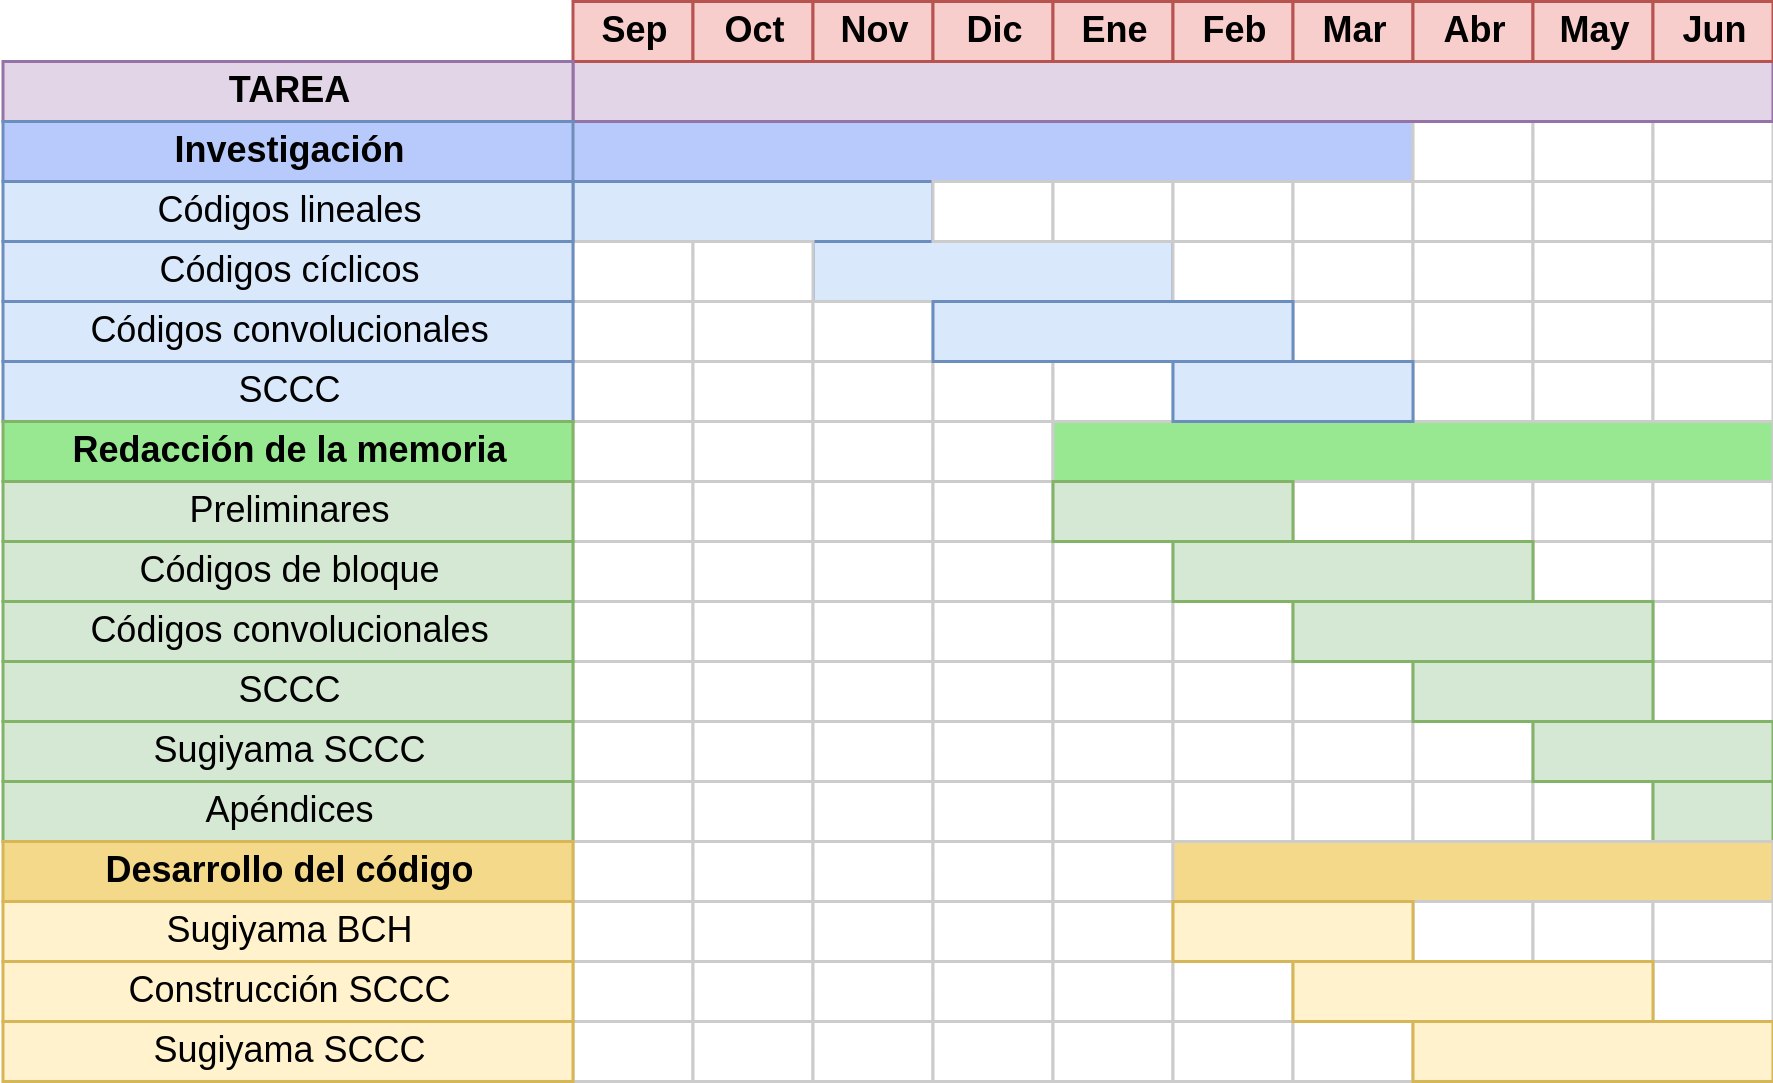
\includegraphics[width=1\textwidth]{img/GRANTT.png}
    \caption{Planificación temporal de las etapas del proyecto.}
    \label{fig:proy}
\end{figure}

\newpage

Vamos a realizar también una aproximación del coste monetario de la creación de este proyecto, considerando su duración de 9 meses. Estos cálculos se realizarán teniendo en cuenta que se han trabajado 450 horas de acuerdo a los 18 créditos ECTS correspondientes asignados al TFG y con un gasto aproximado de 20 €/h.


\begin{small}
    \begin{longtable}{|>{\raggedright\arraybackslash}p{3cm}|>{\raggedright\arraybackslash}p{4cm}|>{\centering\arraybackslash}p{2cm}|>{\centering\arraybackslash}p{2cm}|}
    \hline
    \textbf{Tipo} & \textbf{Tareas} & \textbf{Cantidad (h)} & \textbf{Coste (€)} \\
    \hline
    \endfirsthead
    \hline
    \textbf{Tipo} & \textbf{Tareas} & \textbf{Cantidad (h)} & \textbf{Coste (€)} \\
    \hline
    \endhead
    \hline
    Investigación & Códigos lineales & 30 & 600 \\
    \hline
    Investigación & Códigos cíclicos & 30 & 600 \\
    \hline
    Investigación & Códigos convolucionales & 50 & 1000 \\
    \hline
    Investigación & Códigos convolucionales cíclicos sesgados & 40 & 800 \\
    \hline
    Implementación del código & Sugiyama para BCH & 30 & 600 \\
    \hline
    Implementación del código & Construcción de códigos SCCC & 40 & 800 \\
    \hline
    Implementación del código & Sugiyama para SCCC & 50 & 1000 \\
    \hline
    Redacción de la memoria & Preliminares & 20 & 400 \\
    \hline
    Redacción de la memoria & Códigos de bloque & 50 & 1000 \\
    \hline
    Redacción de la memoria & Códigos convolucionales & 50 & 1000 \\
    \hline
    Redacción de la memoria & SCCC y Sugiyama para SCCC & 60 & 1200 \\
    \hline
    \hline
    \textbf{Total} & & 450 & 9000 \\
    \hline
    \caption{Distribución de tareas y costos}
    \label{tab:costos}
    \end{longtable}
\end{small}
    
La Tabla \ref{tab:costos} se puede observar cuánto tiempo ha requerido cada tarea junto al coste total calculado.

\endinput




% --------------------------------------------------------------------
% GLOSARIO: Opcional
% --------------------------------------------------------------------

%% !TeX root = ../libro.tex
% !TeX encoding = utf8

\chapter*{Glosario}
\addcontentsline{toc}{chapter}{Glosario} % Añade el glosario a la tabla de contenidos

La inclusión de un glosario es opcional.

Archivo: \texttt{glosario.tex}

\begin{description} 
  \item[$\mathbb{R}$] Conjunto de números reales.

  \item[$\mathbb{C}$] Conjunto de números complejos.

  \item[$\mathbb{Z}$] Conjunto de números enteros.
\end{description}
\endinput
 

% -------------------------------------------------------------------
% BACKMATTER
% -------------------------------------------------------------------

\backmatter % Desactiva la numeración de los capítulos
\pdfbookmark[-1]{Referencias e Índices}{BM-Referencias}

% BIBLIOGRAFÍA
%-------------------------------------------------------------------

\setbibpreamble{Las referencias se listan por orden alfabético. Aquellas referencias con más de un autor están ordenadas de acuerdo con el primer autor.\par\bigskip}
\bibliographystyle{plain}
\begin{small} % Normalmente la bibliografía se imprime en un tamaño de letra más pequeño.
  \bibliography{library.bib}
\end{small}


% ÍNDICE TERMINOLÓGICO  (Opcional) 
%------------------------------------------------------------------- 

% Para incluir el índice terminológico es necesario descomentar los siguientes comandos. Incluir un índice terminológico es opcional

% \cleardoublepage 
% \begin{footnotesize} % Normalmente el índice se imprime en un tamaño de letra más pequeño.
% \printindex 
% \end{footnotesize}

\end{document}
